\documentclass[draftthesis,fullpage]{uiucthesis}
\usepackage[utf8]{inputenc}
%\usepackage{fdsymbol}
\setcounter{tocdepth}{4}
\setcounter{secnumdepth}{4}

\usepackage{amsmath,amsfonts,amssymb,amsthm}
\usepackage{graphicx}
\usepackage{braket}
\usepackage{subfiles}
\usepackage{comment}
\usepackage{listings}

\theoremstyle{definition}
\newtheorem{definition}{Definition}[section]
\newtheorem{theorem}{Theorem}[section]

% try bibtex
\usepackage[
backend=bibtex,
citestyle=numeric-comp,
sorting=none
]{biblatex}
\addbibresource{sections/hsolid}
\addbibresource{sections/hcalcs}
\addbibresource{sections/melth2}
\addbibresource{sections/basic}
\addbibresource{sections/books}
\addbibresource{sections/wf}
\addbibresource{sections/fsc}
\defbibheading{general}{\section{References}}
\defbibheading{all}{\chapter{References}}
\addbibresource{papers/licp/licp-ref.bib}
\addbibresource{papers/nonbo/nonbo-ref.bib}

%% try chapter bib
%\usepackage{chapterbib}
%\usepackage[backend=bibtex]{biblatex}

% import figures from difference folders
\usepackage{threeparttable} % for annotated table
\usepackage{siunitx} % for decimal alignment in tables
\usepackage{bm,amssymb,amsmath} % for math
\usepackage[bookmarks]{hyperref} % for reference links
\usepackage[svgnames]{xcolor} % to define color names
\definecolor{Blue}{RGB}{0 0 128}
\hypersetup{ %options-for-appearance-of-links-in-hyperref
	colorlinks= true,
    allcolors = Blue
}
\usepackage{tikz}
\usetikzlibrary{calc} % for tikz calculations
\usetikzlibrary{arrows,decorations.markings} % make arrow head bigger
\usepackage{color,soul} % for reviews
\graphicspath{{./papers/bandgap/},{./papers/nonbo/},{./papers/licp/},
{./papers/hsolid/figures/c2c/},{./papers/hsolid/figures/cmca4/},
{./papers/hsolid/figures/cmca12/},{./papers/hsolid/figures/i41amd/},
{./papers/hsolid/figures/},{./sections/figures/}
}

\newcommand{\toprule}{\hline\hline}
\newcommand{\midrule}{\hline}
\newcommand{\bottomrule}{\hline\hline}
\newcommand{\bs}{\boldsymbol}
\newcommand{\tr}{\text{tr}}
\newcommand{\Tr}[1]{\text{Tr}\left(#1\right)}
\newcommand{\up}{\uparrow}
\newcommand{\dn}{\downarrow}
\newcommand{\ham}{\mathcal{H}}
\newcommand{\veff}{v_{\text{eff}}}

\begin{document}

\title{Electron-ion Correlation and Finite-size Effects in\\
       Quantum Monte Carlo Simulations}
\author{Yubo ``Paul'' Yang}
\department{Physics}
\schools{B.S., Denison University, 2014}
\phdthesis
\advisor{David M. Ceperley}
\degreeyear{2020}
\committee{Assistant Professor Prof B. K. Clark, Chair\\Professor Prof D. M. Ceperley, Director of Research\\Professor Prof J. N. Eckstein\\Professor Prof T. L. Hughes}

% crtl + T to comment; crtl + U to uncomment.
%\maketitle
%\frontmatter

% ProQuest truncates their abstracts at 350 words.
\begin{abstract}
This thesis explores properties of a mixture of electrons and ions using the quantum Monte Carlo method. In many electronic structure studies, purely electronic properties are calculated on a static potential energy surface generated by ``clamped'' ions. This can lead to quantitative errors, for example, in the prediction of diamond carbon band gap, as well as qualitatively wrong behavior, especially when light nuclei such as protons are involved. In this thesis, we explore different ways to include effects of the ions and tackle challenges that arise in the process.
We benchmarked the diffusion Monte Carlo (DMC) method on electron-ion simulations consisting of small atoms and molecules. We found the method to be nearly exact once sufficiently accurate trial wave functions have been constructed. The difference between the dynamic-ion and static-ion simulations can mostly be explained by the diagonal Born-Oppenheimer correction.
We applied this method to solid hydrogen at megabar pressures and tackled additional problems involving geometry optimization and finite-size effects. The phase diagram produced by our electron-ion DMC simulations differ from previous DMC studies, showing $50$ GPa higher molecular-molecular transition and $150$ GPa higher molecular-to-atomic transition pressures. Both aforementioned studies foregone the Born-Oppenheimer approximation (BOA) at hefty computational cost. Unfortunately, this makes it more difficult to compare our results with previous studies performed within the BOA.
The remainder of the thesis tackle finite-size and ionic effects within the BOA. We calculated the Compton profile of solid and liquid lithium, achieving excellent agreement with experiment. Ionic effects of the liquid were included by averaging over disorder atomic configurations. Finite-size correction was crucial for the Compton profile near the Fermi surface. Finally, we tackled the finite-size error in the calculation of band gaps and devised a higher-order correction, which allowed thermodynamic values of the band gap to be obtained from small simulation cells.
These advances mark important points along the path to the exact solution of the electron-ion problem. We expect that the better understanding of both the electron-ion wave function and its relation to finite-size effects obtained in this thesis to be crucial for future simulations of electron-ion systems.
\end{abstract}

\begin{dedication}
To my friends and family.
\end{dedication}

%\chapter*{Acknowledgments}
%This project would not have been possible without the support of many people.
\tableofcontents
%\listoftables
\listoffigures

%% Create a List of Abbreviations. The left column
%% is 1 inch wide and left-justified
\chapter{List of Abbreviations}

\begin{symbollist*}
\item[BOA] Born-Oppenheimer Approximation.
\item[DBOC] Diagonal Born-Oppenheimer Correction.
\item[EOS] Equation Of State.
\item[DM] Density Matrix.
\item[QMC] Quantum Monte Carlo.
\item[RPIMC] Restricted Path Integral Monte Carlo.
\item[VPI] Variational Path Integral.
\item[RMC] Reptation Monte Carlo
\item[FP-DMC] Fixed-Phase Diffusion Monte Carlo.
\item[VMC] Variational Monte Carlo.
\item[KW] Kolos and Wolniewicz.
\item[RHF] Restricted Hartree Fock.
\item[CISD] Configuration Interaction Singles Doubles.
\item[CAS] Complete Active Space.
\item[ANO] Atomic Natural Orbital.
\item[ECG] Explicitly-Correlated Gaussian.
\item[KS-DFT] Kohn-Sham Density Functional Theory.
\item[HK] Hohenberg and Kohn.
\item[LDA] Local Density Approximation.
\item[PZ] Perdew and Zunger.
\item[HOMO] Highest-Occupied Molecular Orbital.
\item[LUMO] Lowest-Unoccupied Molecular Orbital.
\item[PBE] Perdew, Burke, and Ernzerhof.
\item[HSE] Heyd, Scuseria, and Ernzerhof.
\item[SBJ] Slater-Backflow-Jastrow.
\item[RPA] Random Phase Approximation.
\item[RDM] Reduced Density Matrix.
\item[LLT] Liquid-Liquid Transition.
\item[DAC] Diamond Anvil Cell.
\item[MD] Molecular Dynamics.
\item[PES] Potential Energy Surface.
\item[GPa] Giga-Pascal
\item[LP] Low-pressure Phase.
\item[BSP] Broken-Symmetry Phase.
\item[IR] InfraRed.
\item[EQQ] Electric Quadrupole-Quadrupole.
\item[GCTABC] Grand-Canonical Twist Average Boundary Condition.
\item[KZK] Kwee, Zhang, and Krakauer.
\item[MSD] Mean-Squared Deviation.
\item[FWHM] Full Width at Half Max.
\item[SDF] Spectral Density Function.
\item[BFD] Burkatzki, Filippi, and Dolg.
\item[QE] Quantum Espresso.
\item[PPC] PseudoPotential Correction.
\item[FSC] Finite-Size Correction.
\item[BF] Back Flow.
\item[ZPE] Zero-Point Energy.
\end{symbollist*}

%% Create a List of Symbols. The left column
%% is 0.7 inch wide and centered
\chapter{List of Symbols}

\begin{symbollist}[0.7in]
\item[$h$] Planck constant $\hbar=\dfrac{h}{2\pi}$.
\item[$\Psi$] many-body electron-ion wave function.
\item[$\psi$] many-body electron wave function.
\item[$\phi$] one-body electron wave function.
\item[$\chi$] one-body ion wave function.
\item[$\bs{r}_i$] 3D position of electron $i$.
\item[$\bs{r}_I$] 3D position of ion $I$.
\item[$\bs{R}$] positions of all $N$ electrons.
\item[$\bs{R}_I$] positions of all $N_I$ ions.
\item[$\rho$] density matrix or electron density.
\item[$N$] number of electrons.
\item[$N_I$] number of ions.
\item[$\Omega$] total volume.
\item[$L$] linear extent of the simulation cell.
\item[$r_s$] Wigner-Seitz radius.
\item[$k_F$] Fermi wave vector.
\item[$\Gamma$] classical coulomb coupling parameter.
\item[$\beta$] inverse temperature.
\item[$t$] imaginary time unless otherwise specified.
\item[$\tau$] imaginary time step unless otherwise specified.
\item[$Z$] canonical partition function.
\item[$\hat{H}$] electron-ion hamiltonian.
\item[$\ham$] electronic hamiltonian.
\item[$\lambda$] quantumness $\lambda=\dfrac{\hbar^2}{2m}$.
\item[$\Lambda_{kj}$] nonadiabatic coupling between electronic states $k$ and $j$.
\item[$\Lambda$] de Broglie wavelength.
\item[$P$] pressure.
\item[$V$] total potential energy.
\item[$T$] total kinetic energy.
\item[$E$] total energy.
\item[$E_T$] trial total energy.
\item[$\Psi_T$] trial wave function.
\item[$\sigma^2$] variance of the local energy.
\item[$\pi$] probability distribution.
\item[$\Delta$] band gap.
\item[$g(r)$] pair correlation function.
\item[$S(k)$] static structure factor.
\item[$U$] negative exponent of the Jastrow wave function.
\item[$u(r)$] pair contribution to $U$.
\item[$\omega_p$] plasmon frequency.
\item[$\epsilon_{\bs{k}}$] dielectric function.
\item[$n(\bs{k})$] momentum distribution.
\item[$J(p)$] Compton profile.
\end{symbollist}
\mainmatter

%\chapter{Introduction}

Suppose a particle can be described by a probability distribution over space $x$ and time $t$, then the ``uniform'' particle is described by a plane wave
\begin{align}
\psi \propto \exp\left(
i~\dfrac{px-Et}{\hbar}
\right),
\end{align}
with constant momentum $p$ and energy $E$. The imaginary $i$ is needed to keep the amplitude of this wave $\psi^*\psi$ constant, whereas $\hbar$ is needed to remove units from the exponent. From derivatives of this plane wave, it is natural to conjecture the relations of conjugate variables to space and time, i.e. momentum and energy
\begin{align}
\left\{
\begin{array}{l}
\frac{d\psi}{dx} =  i\frac{p}{\hbar}\psi \\ [8 pt]
\frac{d\psi}{dt} = -i\frac{E}{\hbar}\psi
\end{array}
\right. \Rightarrow
\left\{
\begin{array}{l}
p\psi = -i\hbar\frac{d}{dx} \psi \\ [8 pt]
E\psi =  i\hbar\frac{d}{dt} \psi
\end{array}
\right..
\end{align}
Suppose total energy is a sum of non-relativist kinetic energy and local potential energy
\begin{align}
E = \frac{p^2}{2m} + V(x),
\end{align}
then the Hamiltonian operator
\begin{align}
\hat{\mathcal{H}} = \frac{\hat{p^2}}{2m} + V(x) = -\frac{\hbar^2}{2m}\nabla^2 + V(x).
\end{align}

Density matrix
\begin{align}
\rho\propto\exp\left(i\dfrac{S}{\hbar}\right)
\end{align}

\section{The Many-electron Problem}
%\subsection{Hydrogen Atom}
%\subsection{H$_2$ Molecule}
\subsection{Born-Oppenheimer Approximation (BOA)}
\subsection{Beyond the BOA}
\section{Lithium Compton Profile}
\section{Insulator Band Gap}
\section{Outline}

%\chapter{Methods}
%\section{Effective One-Particle Theories}
\subsection{Hartree-Fock}

\newcommand{\hcore}{H^{\text{core}}_{\mu\nu}}
\newcommand{\ksveff}{V^{\text{eff}}_{\mu\nu}}

\subsubsection{The Hartree-Fock Equations}
The Hartree-Fock (HF) equations are a set of linear equations that couple spin orbitals in a determinant wavefunction. They can be obtained by minimizing the energy of a Slater determinant with the constraint that spin orbitals remain orthonormal. If each molecular orbital $a$ is written as a linear combination of a set of basis functions $\{\phi_\mu\}$
\begin{align} \label{eq:hf-psia}
\psi_a = \sum\limits_{\mu=1}^K C_{\mu a} \phi_\mu,
\end{align}
this constraint optimization problem can be converted to a set of linear equations, resulting in an eigenvalue problem.
For a spin-unpolarized system $N_{\up}=N_{\dn}=N/2$, the restricted Hartree-Fock (RHF) solution is defined by the first $N/2$ eigenvectors of the Fock matrix
\begin{align}
F_{\mu\nu} = \hcore + \sum\limits_{\lambda\sigma} P_{\lambda\sigma} \left[
(\mu\nu|\sigma\lambda) - \frac{1}{2}(\mu\lambda|\sigma\nu)
\right],
\end{align} % (3.154)
where $P_{\lambda\sigma}=2\sum_{a=1}^{N/2} C_{\lambda a}C_{\sigma a}^*$ is the density matrix. The integral notation
\begin{align}
(\mu\nu|\lambda\sigma) = \iint d\bs{r}_1 d\bs{r}_2 \phi_\mu^*(\bs{r}_1)\phi_{\nu}(\bs{r}_1)
\frac{1}{\vert\bs{r}_1-\bs{r}_2\vert}
\phi_\lambda^*(\bs{r}_2)\phi_\sigma(\bs{r}_2).
\end{align}
$\hcore$ is the one-electron part of the Hamiltonian expressed in the given basis % (3.149)
\begin{align}
\hcore = \int d\bs{r}_1 \phi_\mu^*(\bs{r}_1)\left(
-\frac{1}{2}\nabla_1^2-\sum\limits_A \dfrac{Z_A}{\vert\bs{r}_1-\bs{R}_A\vert}
\right)  \phi_\nu(\bs{r}_1).
\end{align}
% Q/ How to calculate RHF total energy?
% !!!! NOT the sum of eigenvalues
Since the HF method effectively constructs a trial wave function for the exact electronic hamiltonian, the HF energy is variational
\begin{align}
E_{HF} = \braket{\Psi_{HF}|\ham|\Psi_{HF}} \ge E_0.
\end{align}
The HF equations can be generalized to treat open-shell systems.
If $N_{\up} \neq N_{\dn}$, but the spatial part of each occupied orbital is required to be identical for the $\up$ and $\dn$ electrons. Then, the method is known as resitrcted open-shell HF (ROHF).
If the occupied orbitals are further allowed to differ, then the method is unreistricted (UHF).
An application of RHF to the isolated H$_2$ molecule is detailed in Appendix~\ref{app:mbh2}.

\subsubsection{Basis Set Error}

To obtain ``the'' HF solution, all eigenvectors of the Fock matrix must be included in the span of the basis set used to represent the spin orbitals, i.e. $\{\phi_\mu\}$ in eq.~(\ref{eq:hf-psia}).
In practice, one can approach this \textit{complete basis set limit} by using a sequence of basis sets having increasing size.
The correlation-consistent (cc) basis sets are a widely used standard for this purpose.
The convergence of the total energy of H$_2$ molecule is shown in Fig.~\ref{fig:hf-h2} and compared to an exact references obtained by Kolos and Wolniewicz (KW)~\cite{Kolos1964}.
All calculated energy curves are at least $40$ mha above the exact answer, showing the variational principle at play.
Further, even after basis-set convergece, the RHF energy is still quite different from the exact values.
Besides a trivial overall shift, the HF energy increases at a faster rate at large bond length than the KW curve and overshoots the exact total energy at infinite separation.
This is partly because the two electrons are forced into the same orbital, when they should each reside close to a different proton.
Remarkably, the RHF curve agrees well with the shifted KW curve at the equilibrium bond length $1.4$ bohr and below, suggesting that RHF provides a good description for the exchange interaction among core electrons.
The difference between the exact and RHF energies define the \textit{correlation energy}, because the determinant wave function lacks explicit terms that correlate the electrons.

\begin{figure}[h]
\centering
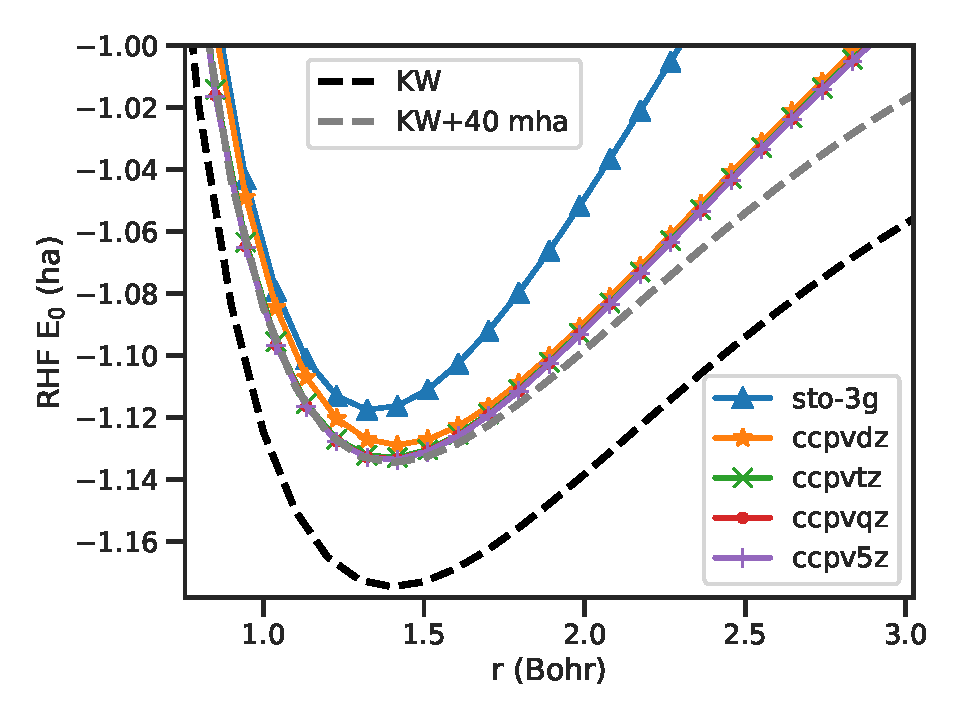
\includegraphics[width=0.6\linewidth]{f19a_h2-rhf-basis}
\caption{RHF electronic ground-state energy of H$_2$ in STO-3G and correlation consistent (cc) basis sets as compared to the exact values calculated by Kolos and Wolniewicz (KW)~\cite{Kolos1964}}
\label{fig:hf-h2}
\end{figure}

\subsubsection{Koopmans Theorem}
HF theory can be used to study electronic excitations from the ground state. Consider removing an electron from orbital $\delta\le N$, the wave function for the $(N-1)$-electron system is~\cite{Giuliani2005}
\begin{align}
\ket{\Psi_{HF}^{(h,\delta)}} = \hat{a}_\delta\ket{\Psi_{HF}}
\end{align}
in the frozen orbital approximation, where the orbitals of the remaining electrons cannot respond to the removed one. The energy of this wave function can be shown to differ from the ground state by $\epsilon_\delta$, the HF eigenvalue of the orbital being emptied.
\begin{align}
E_{HF}^{(h,\delta)} \equiv \braket{\ket{\Psi_{HF}^{(h,\delta)}}|\ham|\ket{\Psi_{HF}^{(h,\delta)}}} = E_{HF} - \epsilon_\delta.
\end{align}
T. Koopmans~\cite{Koopmans1934} first proved this for the highest occupied molecular orbital (HOMO) as an approximation to the ionization energy, although the above derivation is general for any orbital.
Following Chapter 2.2.3 in Ref.~\cite{Giuliani2005}, one can similarly calculate the energy of an N-electron system that differs from the HF ground state by an electron-hole excitation
\begin{align}
\ket{\Psi_{HF}^{(e,\gamma;h,\delta)}} = \hat{a}_\gamma^\dagger \hat{a}_\delta \ket{\Psi_{HF}}, ~\gamma>N,~\delta\le N. \\
E_{HF}^{(e,\gamma;h,\delta)} = E_{HF}+\epsilon_\gamma-\epsilon_\delta-\Delta_{\gamma\delta},
\label{eq:hf-eh}
\end{align}
where $\Delta_{\gamma\delta}>0$. For a stable HF solution, eq.~(\ref{eq:hf-eh}) leads to a \textit{coulomb gap} in the HF density of states in insulators
\begin{align}
N(e) < 2^{d-1}d\left(\dfrac{\epsilon}{e^2}\right)^d(e-e_F)^{d-1},
\end{align}
where $d$ is the number of spatial dimensions, and $\epsilon$ is the dielectric constant of the insulator. That is, the HF density of states must vanish at least as fast as $(e-e_F)^{d-1}$ around the Fermi energy $e_F$.

Koopmans theorem assigns physical meanings to the HF eigenvalues, but is only applicable relative to the HF ground state. For example, one cannot repeatedly apply Koopmans theorem to reconstruct the total energy of the system by stripping one electron at a time. The sum of HF eigenvalues double counts the interaction energy, which must be subtracted to calculate the HF total energy
\begin{align}
E_{HF} = \sum\limits_{\alpha} n_\alpha \epsilon_\alpha - \frac{1}{2}n_\alpha (V_{\alpha\alpha}^{HF}-V_{\alpha\alpha}^{ext}).
\end{align}

\subsubsection{Beyond Hartree-Fock}
Even when the complete basis set limit is reached, the HF solution is still not the exact electronic ground state due to its neglect of electron correlation.
The virtual orbitals can be used to construct N-electron determinants that differ from the HF ground state by changing orbital occupation.
These determinants form a many-body basis, in which any wave function can be expressed as a linear combination.
This leads to the configuration interaction (CI) expansion, where the exact electronic ground state is expanded in many-body bases of increasing sizes
\begin{align} \label{eq:method-hf-ci}
\psi_0 = \lim\limits_{M\rightarrow\infty}\sum\limits_{i=0}^{M} c_i \ket{D_i}.
\end{align}
If all determinants that differs by one particle-hole excitation from reference are considered, then we obtain a CI singles (CIS) expansion. If these, and all determinants with two particle-hole excitations are considered, then the expansion is CI singles and doubles (CISD), etc..

\subsubsection{Static and Dynamic Correlation}
The ground state is said to have \textit{static correlation} if one or more determinants in the exact expansion eq.~(\ref{eq:method-hf-ci}) are nearly degenerate with the reference determinant.
This will happen if there are virtual orbitals nearly degenerate with the highest occupied molecular orbital.
In contrast, the system has \textit{dynamic correlation} if the $c_i$ coefficients are small but non-zero for many determinants with high levels of excitation.
Dynamic correlation is often attributed to strong local correlation such as the electron-electron cusp condition.
The exact definitions of static and dynamic correlations are still murky~\cite{Benavides-Riveros2017}.
I introduce the above working definitions, because the static correlation can be interpreted as a delocalization error due to fractional electron~\cite{Cohen2008}, and is related to the self-interaction error in density functional theory (DFT).
This bridges the languages used in quantum chemistry and condensed matter as well as points to a solution of the infamous ``bandgap problem'', to be introduced in  Sec.~\ref{sec:method-dft-bandgap}.

\subsection{Kohn-Sham Density Functional Theory}
While the Hartree-Fock method enjoys much success in the study of atoms and molecules, its complete neglect of (Coulomb) electron correlation is woefully inadequate for many solids. The total energy is dominated by inner shell contributions, which overshadow the valence contributions important for bonding and correlated excitations in solids. The HF energy eigenvalues show vanishing density of states at the Fermi level in metals and unphysically large band gaps in insulators~\cite{Perdew1981}.

Density functional theory uses the three-dimensional total electron density $n(\bs{r})$ as the basic variable rather than the 3N-dimensional many-body wave function $\Psi(\bs{r}_1,\dots,\bs{r}_N)$. This is a dramatic simplification that likely lead to its dominance in modern electronic structure theory of solids and material science.

\subsubsection{The Hohenberg-Kohn theorems}
While having roots in Thomas-Fermi theory~\cite{Parr1989}, DFT was put on firm theoretical foundation by P. Hohenberg and W. Kohn (HK) in 1964~\cite{Hohenberg1964}, where they calculate the total energy $E$ from an external potential $v(\bs{r})$ and a functional of the ground-state electron density
\begin{align}
E\equiv \int d\bs{r} n(\bs{r}) v(\bs{r}) + F[n(\bs{r})].
\end{align}
Two theorems are often attributed to this work:
\begin{definition}
\textit{V-representable density} A density $n(\bs{r})$ is V-representable if it is the ground-state density of some Hamiltonian $H$ in an external potential $v(\bs{r})$.
\end{definition}
\begin{theorem}
Assuming non-degenerate ground state, any V-representable ground-state density $n(\bs{r})$ uniquely determines its external potential $v(\bs{r})$. %(See extension to N-representable density by M. Levy)
\end{theorem}
\begin{proof}
by contradiction: Suppose there are two distinct external potentials $v$ and $v'$ that give rise to the same density $n$ via different hamiltonians $H$, $H'$ and wave functions $\Psi$ and $\Psi'$, respectively. By the variational principle $\braket{\Psi'|H'|\Psi'}+\braket{\Psi'|v'-v|\Psi'}=\boxed{\braket{\Psi'|H|\Psi'}>\braket{\Psi|H|\Psi}}=\braket{\Psi|H'|\Psi}+\braket{\Psi|v'-v|\Psi}>\braket{\Psi'|H'|\Psi'}+\braket{\Psi|v'-v|\Psi}$. Since $\Psi$ and $\Psi'$ give the same density, the local term $\braket{v'-v}$ cancels to give $\braket{\Psi'|H'|\Psi'}>\braket{\Psi'|H'|\Psi'}$, which is a contradiction.
\end{proof}
\begin{theorem}
Assuming number-conserving density variations that retain V-representability, the energy functional has a unique minimum at the ground-state density.
\end{theorem}
\begin{proof}
Consider an external potential $v$, its hamiltonian $H$, and its unique ground state $\Psi$ and density $n$. After a number-conserving variation, the new wave function $\Psi'$ can be used with the original hamiltonian and $\braket{\Psi'|H|\Psi'}>\braket{\Psi|H|\Psi}$ by the variational principle.
\end{proof}

These initial proofs by HK have two important assumptions: 1. the ground-state is non-degenerate and 2. the electron density $n(\bs{r})$ is V-representable. The latter is especially sever because reasonable densities were shown to be not V-representable~\cite{Levy1982,Lieb1983}. Fortunately, M. Levy proved that both assumptions can be weakened~\cite{Levy1979}.
\begin{definition}
\textit{N representable density} A density $n(\bs{r})$ is N-representable if it can be obtained from some anti-symmetric wave function.
\end{definition}
The HK theorems hold for N-representable densities regardless of ground-state degeneracy.

While less publicized, HK also pointed out that the exact density functional less the direct/Column contribution can be calculated from a local energy-density functional $g_{\bs{r}}[n]$
\begin{align}
G[n]\equiv F[n]-\frac{1}{2}\int d\bs{r}d\bs{r}' \dfrac{n(\bs{r})n(\bs{r}')}{\vert\bs{r}-\bs{r}'\vert}=\int \bs{r} g_{\bs{r}}[n],\\
g_{\bs{r}}[n] \equiv \frac{1}{2}\nabla_{\bs{r}}\nabla_{\bs{r}'} n_1(\bs{r}, \bs{r}')\vert_{\bs{r}=\bs{r}'}+
\frac{1}{2}\int d\bs{r}' \dfrac{C_2(\bs{r}-\bs{r'}/2;\bs{r}+\bs{r}'/2)}{\vert\bs{r}'\vert},
\end{align}
which is constructed from one- and two-body reduced density matrices $n_1$ and $C_2$. They even went as far as to relate the leading-order behavior of the density functional to polarizability
\begin{align}
G[n] = G[n_0] + \int d\bs{r}d\bs{r}' K(\bs{r}-\bs{r}')\tilde{n}(\bs{r})\tilde{n}(\bs{r}')+h.o.,
\end{align}
where $\tilde{n}$ is a small number-conserving density variation and the kernel $K$ is related to the polarizability in reciprocal space
\begin{align}
K(\bs{r}-\bs{r}') = \dfrac{1}{\Omega}\sum\limits_{\bs{q}} K(\bs{q}) e^{-i\bs{q}\cdot(\bs{r}-\bs{r}')}, \\
K(\bs{q}) = \dfrac{2\pi}{q^2}\left[ \frac{1}{\alpha(\bs{q})}-1 \right] = \dfrac{2\pi}{q^2}\dfrac{1}{\epsilon(\bs{q})},
\end{align}
where $\alpha(\bs{q})$ and $\epsilon(\bs{q})$ are the polarizability and dielectric constant, respectively. The HK theorems and limits provide some checks for practical parametrization of the exact density functional. Unfortunately, they provide no guidance on how one might start to construct numerical approximations to the exact functional.

\subsubsection{The Kohn-Sham equations}

One year after HK, W. Kohn and L. J. Sham (KS)~\cite{Kohn1965} worked out practical guidelines for constructing approximations to the exact density functional. KS first partitioned the total energy to highlight the least-understood ``exchange-correlation" term $E_{xc}[n]$.
\begin{align} \label{eq:ks-etot}
E=\int d\bs{r} n(\bs{r}) v(\bs{r}) + \frac{1}{2}\int d\bs{r}d\bs{r}' \dfrac{n(\bs{r})n(\bs{r}')}{\vert\bs{r}-\bs{r}'\vert} + T[n] + E_{\text{xc}}[n],
\end{align}
where $T$ is a kinetic energy functional. KS then approximated $E_{xc}$ by the corresponding contribution in the homogeneous electron gas, the local density approximation (LDA)
\begin{align}
E_{\text{xc}}[n] = \int d\bs{r}n(\bs{r})\epsilon_{\text{xc}}(n(\bs{r})).
\end{align}
Next, by minimizing eq.~(\ref{eq:ks-etot}) with respect to number-conserving density variation, they obtained the stationary condition for the ground-state density
\begin{align}
\int \delta n \left[
\dfrac{\delta T[n]}{\delta n}+
v(\bs{r}) + \int d\bs{r}' \dfrac{n(\bs{r}')}{\vert\bs{r}-\bs{r}'\vert}+
\dfrac{d(n\epsilon_{\text{xc}}(n))}{dn}
\right] = 0. \label{eq:ks-dn}
\end{align}
To solve eq.~(\ref{eq:ks-dn}), KS \textit{assumed} that the ground-state density $n$ came from an auxiliary system of non-interacting electrons, i.e., a Slater determinant. This KS \textit{ansatz} turns eq.~(\ref{eq:ks-dn}) into a system of one-particle equations of non-interacting particles in some effective potential $v^{\text{eff}}_{KS}$ determined by the density $n(\bs{r})$. Most practical implementations of DFT use the KS auxiliary-system formulation.

Practical success of the DFT LDA method was not realized until 1981, when J. P. Perdew and A. Zunger~\cite{Perdew1981} (PZ) parametrized exact quantum Monte Carlo data of the homogeneous electron gas, obtained by D. M. Ceperley and B. J. Alder~\cite{Ceperley1980} the year prior. PZ's eq.~(13-17) define the KS-DFT method and the LDA we use today. The electron density for spin $\sigma$ is a sum of occupied spin orbitals squared
\begin{align}
n_{\sigma} = \sum\limits_{\sigma}\sum\limits_{a=1}^{N_{\sigma}}
f_{a\sigma} \vert\psi_{a\sigma}(\bs{r})\vert^2,
\end{align}
where the occupation numbers $f_{a\sigma}\in[0, 1]$, and the kinetic energy is the sum of contributions from all occupied spin orbitals
\begin{align}
T[n] = \sum\limits_\sigma\sum\limits_{a=1}^{N_{\sigma}}
f_{a\sigma} \braket{\psi_{a\sigma}|-\frac{1}{2}\nabla^2|\psi_{a\sigma}}.
\end{align}
Minimizing eq.~(\ref{eq:ks-etot}) with the constraint that the spin orbitals remain orthonormal, PZ obtains
\begin{align}
\dfrac{\delta}{\delta\psi_{a\sigma}} \left[
T[n] + \int d\bs{r}v(\bs{r}) + \int d\bs{r}\int d\bs{r}' \dfrac{n(\bs{r}')}{\vert\bs{r}-\bs{r}'\vert} +
\dfrac{\delta}{\delta n_{\sigma}} E_{xc}(n_{\up},n_{\dn})
\right].
\end{align}

\subsubsection{The Band Gap Problem} \label{sec:method-dft-bandgap}
The Kohn-Sham eigenvalues do not have the same physical meaning as the Hartree-Fock eigenvalues as given by Koopmans theorem. Thus, a band gap ``problem'' arises when one compares the HOMO-LUMO gap from KS-DFT to experimental measurements of the fundamental gap $E_g$.

The eigenvalue of the Kohn-Sham HOMO can be identified with the ionization energy of an isolated molecule if the exchange-correlation potential vanish at infinity.
In this case, the ionization energy is dominated by the long-range asymptotic behavior of the 1RDM, which is determined by the long-range tail of the electronic density with no contribution from the short-sighted exchange correlation potential.

When extended to handle systems with fractional electron number, the derivative discontinuity of the exact density functional is equal $E_g$. It has contribution from both the non-interacting kinetic functional $T_s[n]$ and the exact exchange-correlation functional $E_{xc}[n]$. The KS HOMO-LUMO gap measures the derivative discontinuity in $T_s[n]$. However, as shown in Fig.~\ref{fig:method-dft-smooth-lda}, in the LDA, $E_{xc}[n]$ is smooth, so its contribution to the gap is missing. As a result, the LDA gap is $\sim 50\%$ that of experiment, showing that the derivative discontinuity in $E_{xc}[n]$ can be of similar magnitude as the gap and cannot be ignored.

\begin{figure}[h]
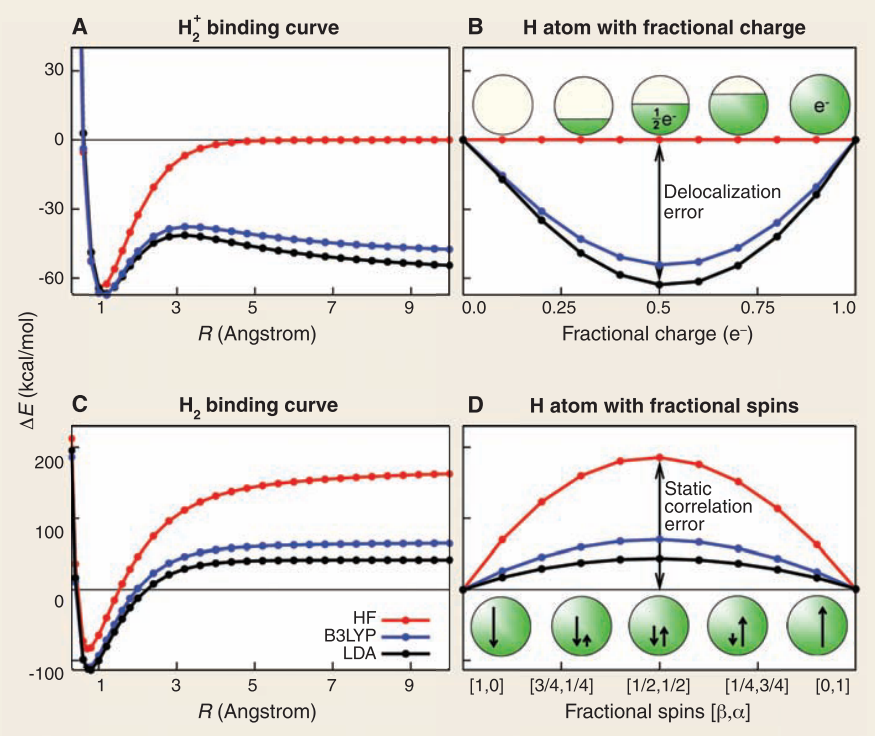
\includegraphics[width=0.45\linewidth]{cohen2008-fig1}
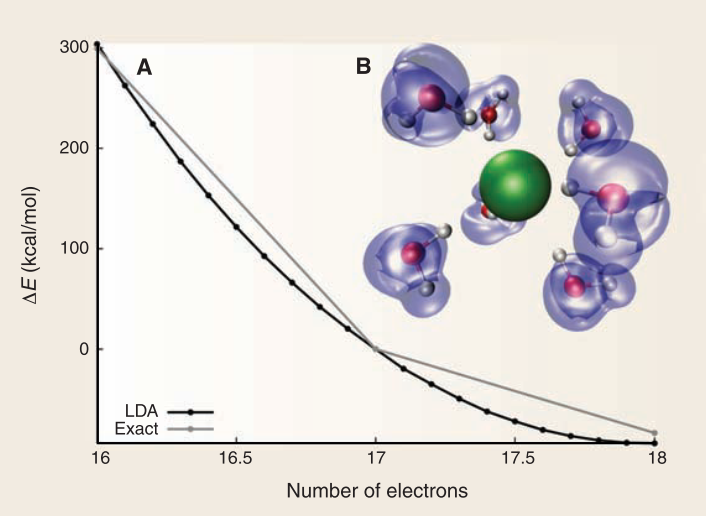
\includegraphics[width=0.52\linewidth]{cohen2008-fig2}
\caption{A. J. Cohen, P. Mori-S\'anchez, and W. Yang~\cite{Cohen2008} explains the self-interaction error in H$_2$ binding curve (left panel C and D) due to the presence of fractional electron (left panel B), which leads to a delocalization error when LDA is used (right panel).}
\label{fig:method-dft-smooth-lda}
\end{figure}

% Q/ why is HSE so good?
% A/ because it has both convex and concave components. See Cohen 2008 Fig. 2

\subsubsection{Beyond Local Density Approximation}

While extremely successful, the LDA has well-documented deficiencies. LDA underestimates the band gap due to a lack of derivative discontinuity as discussed in the previous Sec.~\ref{sec:method-dft-bandgap}. LDA tends to overestimate the binding energy of molecular systems. This is attributed to the logarithmic divergence of the LDA correlation functional as density tends to infinity (see eq.~(7.55) in Ref.~\cite{Giuliani2005}).
%For an isolated atom, the LDA xc potential approaches zero exponentially fast at large distances rather than the correct asymptotic limit $-e^2/r$.

The logarithmic divergence of the LDA is largely corrected by the generalized gradient approximation (GGA). This modification is as straight-forward as adding an extra term that depends on the gradient of the electron density $\bs{\nabla}n$ to the exchange-correlation function. An arbitrary choice of the gradient term can distort the xc hole and break the sum rule that controls its global strength
\begin{align}
\int\bs{r}' n(\bs{r}')[g(\bs{r},\bs{r}')-1] = -1.
\end{align}
J. Perdew and co-workers overcame this difficulty by introducing a real-space cutoff to the exchange hole. While the details are technical, the final form of the GGA exchange functional is elegant
\begin{align} \label{eq:method-dft-pbe-x}
E_x^{GGA}[n] = \int d\bs{r} n(\bs{r})\epsilon_x(n(\bs{r}))F_x(\bs{s}(\bs{r})),
\end{align}
where $\epsilon_x$ is the LDA exchange function and the scaled gradient
\begin{align}
\bs{s}(\bs{r}) = \dfrac{\bs{\nabla}n(\bs{r})}{2k_F(\bs{r})n(\bs{r})}.
\end{align}
A simple form for the exchange enhancement factor $F_x$ was given by J. Perdew, K. Burke, and E. Ernzerhof in 1996. After another careful cutoff on the correlation functional, the immensely popular PBE functional was constructed. The PBE xc functional takes the same form as eq.~(\ref{eq:method-dft-pbe-x}), but with a different enhancement factor $F_{xc}$ instead of $F_x$.
PBE softens molecular bonds relative to the LDA and predict an order of magnitude more accurate dissociation energies of many molecules~\cite{Perdew1996}.

Another well-known failure of local and semi-local density functional theory is the absence of Van der Waals interaction.
This interaction is entirely due to the correlation of density fluctuations and is dominant for two non-overlapping electron densities.
When fluctuation creates an instantaneous dipole moment in one electron distribution, it induces an anti-aligned dipole moment in the other.
The Van der Waals interaction is thus attractive and decays as $\frac{1}{r^6}$ in the separation distance $r$ between the centers of the two distributions.
While KS-DFT relies on the average electron density of a non-interacting system, it is still possible to include the contribution of Van der Waals interaction in the density functional.
Consider the Coulomb interaction as a perturbation to two widely separated atoms, one can show that the interaction energy is proportional to a convolution of the density-density response functions of the isolated atoms
\begin{align}
\braket{\hat{H}_{12}} = -\dfrac{\hbar}{2\pi}
\int d\bs{r}_1d\bs{r}_1'
\int d\bs{r}_2d\bs{r}_2'
\dfrac{e^2}{\vert\bs{r}_1-\bs{r}_2\vert}
\dfrac{e^2}{\vert\bs{r}_1'-\bs{r}_2'\vert} \nonumber \\
\times\int\lim\limits_0^{\infty}
\chi_1(\bs{r}_1, \bs{r}_1')
\chi_2(\bs{r}_2, \bs{r}_2') + h.o.,
\end{align}
as written in eq~.(7.116) in Ref.~\cite{Giuliani2005}. One can then proceed to approximate the density-density response function using the static electron density, for example using the polarizability of the homogeneous electron gas.

Finally, exact-exchange functionals such as PBE0 and HSE~\cite{Heyd2003} have been developed for atoms having localized valence electrons, e.g., with d or f angular momentum.
These functionals are crucial in the study of magnetism, as PBE functional overly favor delocalized electrons and often predict qualitatively wrong magnetic momentum and spin orderings of transition metals.
However, these functionals were never a focus throughout this thesis, so I will not go into details here.
%exact exchange functionals (HSE)
%SCAN?
%\section{Classical Monte Carlo}
The Monte Carlo methods mentioned in this thesis perform high-dimensional integrals by using random numbers to sample probability distributions. These distributions must be non-negative in the entire domain of ``states'' over which they are defined. In classical mechanics, a ``state'' of N particles is labeled by the positions $\bs{r}\equiv\{\bs{r}_i\}$ and momenta $\bs{p}\equiv\{\bs{p}_i\}$ of the particles $i=1,\dots,N$. The classical partition function for the canonical ensemble
\begin{align} \label{eq:classical-nvt-part}
Z \equiv \text{Tr}(e^{-H/k_BT}) = \dfrac{1}{N!h^{3N}} \int d\bs{r} d\bs{p} e^{-H(\bs{r}, \bs{p})/k_BT},
\end{align}
where $H(\bs{r}, \bs{p})$ is the hamiltonian, $k_B$ is the Boltzmann constant, $h$ is the Planck constant, and $T$ is temperature. For $N$ distinguishable non-relativistic particles with mass $m$, the kinetic contribution $\dfrac{p^2}{2m}$ to eq.~(\ref{eq:classical-nvt-part}) can be integrated analytically, giving
\begin{align}\label{eq:classical-nvt-part-v}
Z = \dfrac{1}{N!\Lambda^{3}} \int d\bs{r} e^{-\beta V(\bs{r})},
\end{align}
where $V(\bs{r})$ is the potential energy of the system, $\beta\equiv k_BT$, and $\Lambda$ the de Broglie wavelength
\begin{align} \label{eq:debroglie}
\Lambda = \left(
\dfrac{h^2}{2\pi mk_BT}
\right)^{1/2}.
\end{align}

All equilibrium statistical mechanics properties can be calculated from the partition function, so the entirety of classical equilibrium statistical mechanics reduces to the problem of evaluating the 3N-dimensional integral in eq.~(\ref{eq:classical-nvt-part-v}) and its derivatives. Monte Carlo methods are ideally suited to evaluating high-dimensional integrals, because the amount of computation does not increase as an exponential in the number of dimensions as in a brute-force quadrature approach.

To calculate a property in the canonical ensemble, ones takes the trace
\begin{align}
\braket{O} = \dfrac{\Tr{Oe^{-\beta H}}}{\Tr{e^{-\beta H}}},
\end{align}
where $\braket{}$ denotes ensemble average. Limiting to local observables that can be evaluated on the particle coordinates, e.g., total potential energy $V(\bs{r})$ and pair correlation function $g(r)$
\begin{align} \label{eq:int-obs}
\braket{O} = \int d\bs{r} \dfrac{e^{-\beta V(\bs{r})}}{\int d\bs{r}' e^{-\beta V(\bs{r}')}} O(\bs{r}) = \int d\bs{r} \pi(\bs{r})O(\bs{r}),
\end{align}
where $\pi(\bs{r})$ is the Bolzmann distribution
\begin{align} \label{eq:bolzmann-pi}
\pi(\bs{r}) \equiv \dfrac{e^{-\beta V(\bs{r})}}{\int d\bs{r}' e^{-\beta V(\bs{r}')}} \propto e^{-\beta V(\bs{r})}.
\end{align}
Monte Carlo estimation of $\braket{O}$ works by sampling particle configurations from the Bolzmann distribution $\pi(\bs{r})$ and accumulating the average $O(\bs{r})$
\begin{align}
\braket{O} = \lim\limits_{N_s\rightarrow\infty} \frac{1}{N_s} \sum\limits_{i=1}^{N_s} O(\bs{r}_i).
\end{align}
How does one sample a generic probability distribution such as $\pi(\bs{r})$?
An excellent answer was given a 1953 paper authored by Metropolis \textit{et al.}~\cite{Metropolis1953}. The Metropolis algorithm, worked out by the Rosenbluths supervised by the Tellers, works by constructing a Markov chain having $\pi(\bs{r})$ as its stationary state. This is achieved by a rejection method that maintains detailed balance
\begin{align} \label{eq:detailed-balance}
\pi(\bs{r})P(\bs{r}\rightarrow\bs{r}')=\pi(\bs{r}')P(\bs{r}'\rightarrow\bs{r}),
\end{align}
where $P(\bs{r}\rightarrow\bs{r}')$ is the Markov chain transition probability from state $\bs{r}$ to $\bs{r}'$. The Metropolis algorithm breaks $P$ into two steps: proposal and acceptance
\begin{align} \label{eq:metropolis-prob}
P(\bs{r}\rightarrow\bs{r}') = T(\bs{r}\rightarrow\bs{r}')A(\bs{r}\rightarrow\bs{r}'),
\end{align}
with the following accept/reject criteria: For any transition probability used to propose the state change $T(\bs{r}\rightarrow\bs{r}')$, accept the change with probability
\begin{align} \label{eq:metropolis-accept}
A(\bs{r}\rightarrow\bs{r}') = \min\left(1, \dfrac{\pi(\bs{r}')T(\bs{r}'\rightarrow\bs{r})}{\pi(\bs{r})T(\bs{r}\rightarrow\bs{r}')}\right).
\end{align}
Using eq.~(\ref{eq:metropolis-prob}) and (\ref{eq:metropolis-accept}) to prove eq.~(\ref{eq:detailed-balance}) is a good way to appreciate the design of this acceptance probability.

Mathematically, $\pi(\bs{r})$ is the unique stationary state of the Markov chain constructed by the Metropolis method so long as $P(\bs{r}\rightarrow\bs{r}')$ is ergodic. That is, there is finite probability of reaching any state $\bs{r}'$ starting from any state $\bs{r}$ using $P$.
In practice, however, a simulation can be stuck in a meta-stable state for its entire duration, for example, due to a bad initial condition. Careful monitoring and checking of convergence is a must in any serious Monte Carlo simulation.

\section{Quantum Monte Carlo}

%A typical introduction to quantum Monte Carlo (QMC) starts with the oldest and simplest method variation Monte Carlo (VMC), then work its way to diffusion Monte Carlo (DMC) and path integral Monte Carlo.
I will start with the general, albeit somewhat complicated, path integral Monte Carlo (PIMC) method, because it rigorously takes temperature into account and connects well with classical Monte Carlo. Then, I will describe ground-state methods as limits and efficiency tricks to specialize the path integral method to the ground state. While contrary to the historic progression of these methods, I find this perspective helpful for relating the methods and visualizing them in their respective niches.

\subsection{Path Integral Monte Carlo (PIMC)}
The quantum partition function for the canonical ensemble needs to trace over discrete N-particle eigenstates, rather than 2N 3-dimensional variables as in eq.~(\ref{eq:classical-nvt-part})
\begin{align}
Z\equiv \text{Tr}(e^{-H/k_BT})=\text{Tr}\left(
\sum\limits_{i=1}^{\infty} e^{-E_i/k_BT}\ket{\Psi_i}\bra{\Psi_i}
\right),
\end{align}
where $E_i$ and $\ket{\Psi_i}$ are the eigenvalues and eigenstates of the hamiltonian $H$. To make contact with classical mechanics, we put the density matrix (DM) for distinguishable particles in position basis (first quantization)
\begin{align}
\rho_D(\bs{r}, \bs{r}'; \beta) \equiv \braket{r|e^{-\beta H}|r'},
\end{align}
where $\beta\equiv \frac{1}{k_B T}$. 
Then the partition function becomes
\begin{align} \label{eq:quantum-nvt-zd}
Z(\beta) = \int d\bs{r} \rho_D(\bs{r},\bs{r};\beta),
\end{align}
which can be exactly factorized into two pieces
\begin{align}
Z(\beta) = \int d\bs{r}d\bs{r}' \rho_D(\bs{r},\bs{r};\tau)\rho_D(\bs{r},\bs{r};\beta-\tau).
\end{align}
This factorization can be repeated until the temperature becomes high enough ($\tau\rightarrow0$) that a semi-classical approximation to $\rho_D(\bs{r},\bs{r}';\tau)$ is accurate. Given translation symmetry along imaginary time, $\beta$ is typically broken down into $M$ equal-length pieces, i.e., $\tau=\beta/M$.
For $N$ non-relativistic particles each having mass $m$, $\rho_D$ can be calculated as an integral over a discretized ``path'' of particle coordinates $\{\bs{r}_m\}$
\begin{align} \label{eq:pimc-rhod}
\rho_D(\bs{r}_0,\bs{r}_M;\beta) = \lim\limits_{M\rightarrow\infty} \int d\bs{r}_1\dots d\bs{r}_{M-1}
(4\pi\lambda\tau)^{-dNM/2}\exp\left(
-\sum\limits_{m=1}^M \left[
\dfrac{(\bs{r}_{m-1}-\bs{r}_m)^2}{4\lambda\tau} + \tau V(\bs{r}_m)
\right]
\right),
\end{align}
where $\lambda\equiv\dfrac{\hbar^2}{2m}$ is the ``quantumness'' of the particle and $d$ is the number of spatial dimensions. Thus, the partition function eq.~(\ref{eq:quantum-nvt-zd}) becomes an integral of a product of high-temperature DMs over all closed paths
\begin{align} \label{eq:quantum-nvt-zd-pi}
Z=\lim\limits_{M\rightarrow\infty} \int d\bs{r} d\bs{r}_1\dots d\bs{r}_{M-1}
\rho_D(\bs{r},\bs{r}_1;\tau)\rho_D(\bs{r}_1,\bs{r}_2;\tau)\dots\rho_D(\bs{r}_{M-1},\bs{r};\tau).
\end{align}
Each closed path can be visualized as a collection of ring polymers, one for each particle. The linear extension of a ring polymer is proportional to the particle's de Broglie wavelength $\Lambda=\sqrt{4\pi\lambda\beta}$ eq.~(\ref{eq:debroglie}).
For distinguishable particles, the integral needed to evaluate the quantum partition function eq.~(\ref{eq:quantum-nvt-zd-pi}) poses no essential difficulty to a Monte Carlo method when compared with its classical counterpart eq.~(\ref{eq:classical-nvt-part-v}). One simply has to integrate $M$ classical systems, which are coupled by the spring-like kinetic energy term in eq.~(\ref{eq:quantum-nvt-zd}).
% a technical difficult for bosons -> permutation moves
However, if the particles are identical bosons (fermions pose an essential problem, see Sec.~\ref{sec:fermion-sign-problem}), then one has to consider particle permutations along the path
\begin{align}
\rho_B(\bs{r}_0,\bs{r}_M;\beta) = \frac{1}{N!}\sum\limits_{\mathcal{P}} \rho_D(\bs{r}_0, \mathcal{P}\bs{r}_M;\beta),
\end{align}
where $\mathcal{P}\bs{r}_M$ contains the same $N$ coordinates as $\bs{r}_M$, but with the particles relabeled. This permutation can happen via any number of 1-, 2-, and up to $N$-particle exchanges between adjacent time slices along the path. Thus, the state space of bosonic path integral is much larger than that of boltzmannic path integral. Efficient sampling of permuting paths is a significant technical challenge. Fortunately, no uncontrolled approximation has been introduced and exact simulations are possible for both bolzmannons and bosons via the Monte Carlo method.

\subsection{Variation Path Integral a.k.a. Reptation Monte Carlo}
% ground-state path integral (VPI) -> RMC
% i.e. use a trial wavefunction as link action
The ground state is costly to study using the path integral formalism presented so far, because a large number of time slices have to be included to approximate $\beta\rightarrow\infty$. Fortunately, one can still efficiently study the ground state with the help of a trial wave function $\ket{\Psi_T}$, so long as it is non-negative. The ground-state ``partition'' function has only one term
\begin{align}
Z_0 = \lim\limits_{\beta\rightarrow\infty} \braket{\Psi_0|e^{-\beta H}|\Psi_0},
\end{align}
where $\ket{\Psi_0}$ is the ground state of the hamiltonian $H$.
For sufficiently large $\beta$, any trial wave function not orthogonal to the ground state $\braket{\Psi_T|\Psi_0}\neq0$ will be projected to the ground state by $e^{-\beta H}$, so
\begin{align} \label{eq:rmc-z0}
Z_0 = \lim\limits_{\beta\rightarrow\infty}\braket{\Psi_T|e^{-\frac{\beta}{2} H}e^{-\frac{\beta}{2} H}|\Psi_T} \approx \braket{\Psi_T|e^{-\beta_e H}e^{-\beta_e H}|\Psi_T},
\end{align}
for some $\beta_e$ large enough to be considered ``equilibrated''. Performing path discretization as before
\begin{align} \label{eq:pimc-vpi-z0}
Z_0 = \lim\limits_{M\rightarrow\infty} \int d\bs{r}_{-M}\dots d\bs{r}_0\dots d\bs{r}_{M}
\Psi_T^*(\bs{r}_{-M})\rho(\bs{r}_{-M},\bs{r}_{-M+1};\tau)\dots\rho(\bs{r}_{M-1},\bs{r}_M;\tau)\Psi_T(\bs{r}_M),
\end{align}
where $\tau=\beta_e/M$. $\beta_e$ can be small if $\ket{\Psi_T}$ is a good approximate to the ground state $\ket{\Psi_0}$. In this sense, $\ket{\Psi_T}\bra{\Psi_T}$ plays the role of a low-temperature density matrix to quickly close a long path, although its temperature is ill-defined. No permutation needs to be sampled because quantum statistics are encoded in the trial wave function. However, translation symmetry along imaginary time is broken. The 2M+1 time slices each sample a different probability distribution. Observables that do not commute with the hamiltonian are unbiased only when evaluated on the middle slice $\bs{r}_0$. The trial wave functions at the ends and the DMs in the middle of eq.~(\ref{eq:pimc-vpi-z0}) must all be non-negative for the integrand to be interpreted as a probability distribution for the path $\{\bs{r}_{-M},\dots,\bs{r}_M\}$. This path is, in general, open ($\bs{r}_{-M}\neq\bs{r}_M$) and can be visualized as a ``reptile''. This method was first mentioned as variational path integral (VPI)~\cite{Ceperley1995}, but later popularized as reptation Monte Carlo (RMC)~\cite{Baroni1999}. While the RMC method can be efficient, it still requires all $M$ classical systems to be stored in memory at one time and intelligent Monte Carlo moves to change the reptile without ergodicity problems. This makes RMC much more troublesome to implement than classical Monte Carlo or molecular dynamics.

\subsection{Diffusion Monte Carlo}
The diffusion Monte Carlo (DMC) method can be viewed as a simplification of RMC.
When calculating a ground-state observable using eq.~(\ref{eq:rmc-z0}), the \emph{pure estimator}
\begin{align} \label{eq:dmc-opure}
\braket{\hat{O}}_p \equiv \braket{\Psi_T|e^{-\beta_e H}\hat{O}e^{-\beta_e H}|\Psi_T} \approx \braket{\Psi_0|\hat{O}|\Psi_0}
\end{align}
is an unbiased ground-state estimate of $\hat{O}$ whether it commutes with the hamiltonian or not. We can forgo the pure estimator for a simpler algorithm. Consider the \emph{mixed estimator}
\begin{align} \label{eq:dmc-omixed}
\braket{\hat{O}}_m \equiv \braket{\Psi_T|\hat{O}e^{-\beta_e H}|\Psi_T}\approx\braket{\Psi_T|\hat{O}|\Psi_0}.
\end{align}
Equation~(\ref{eq:dmc-omixed}) has the advantage that the operator can be immediately applied to a trial wave function, which is known at the beginning of the calculation. Further, the $\Psi_0$ on the r.h.s. can be interpreted as being propagated from $\Psi_T$ using the \emph{imaginary-time propagator}
\begin{align}
\hat{U}(t) = e^{-t H}.
\end{align}
For any $t>\beta_e$, the observable value eq.~(\ref{eq:dmc-omixed}) should be stationary. The algorithm as described so far is similar to classical molecular dynamics. One starts with a trial wave function at $t=0$ and propagates it along imaginary time. After some initial equilibration period, the mixed estimator fluctuates around some stationary mean. One then runs for ``longer'' and accumulate statistics.

%For non-relativistic particles, $\nabla^2$ in the kinetic energy operator turns into a Green function for diffusion $e^{-t\nabla^2}$.
For identical non-relativistic particles having mass $m$, $\hat{U}$ in coordinate basis is the Green function for imaginary-time Schr\"odinger equation
\begin{align}
G(\bs{r}'\leftarrow\bs{r};t) = \braket{\bs{r}'|\hat{U}(t)|\bs{r}} =  \braket{\bs{r}'|e^{-t(\lambda \nabla^2+V)}|\bs{r}} = \lim\limits_{\tau\rightarrow 0}
\left(
(4\pi\lambda\tau)^{-dN/2}e^{-\dfrac{(\bs{r}-\bs{r}')^2}{4\lambda\tau}}
\right)
\left(
e^{-\tau V(\bs{r})}
\right). \label{eq:dmc-green}
\end{align}
The two terms in eq.~(\ref{eq:dmc-green}) are the Green function for diffusion and weight accumulation.
The quantumness $\lambda=\frac{\hbar^2}{2m}$ of the particle determines its diffusion constant in imaginary time. Lighter particles diffuse ``faster''. One can, in principle, start with any classical system $\bs{r}$, apply the Green functions repeatedly to update $\bs{r}$, and eventually end up sampling the mixed distribution $\braket{\Psi_T|\Psi_0}$.

While eq.~(\ref{eq:dmc-omixed})-(\ref{eq:dmc-green}) contain the main idea behind the DMC method, they do not result in a practical algorithm. The weight of the classical system due to the potential term goes to zero or infinity exponentially fast whenever two charged particles coalesce. For a stable algorithm, one can modify the Green function eq.~(\ref{eq:dmc-green}) to more directly sample the mixed distribution
\begin{align}
f(\bs{r},t) \equiv \Psi_T^*(\bs{r}) e^{-t(H-E_T)}\Psi_T(\bs{r}) \underset{t\rightarrow\infty}{=} \Psi_T^*(\bs{r})\Psi_0(\bs{r}),
\end{align}
where a trial energy $E_T$ is introduced to stablize the potential term.
Substitute $\Psi_T^{-1}f$ in place of $\Psi$ into the imaginary-time Schr\"odinger equation $-\partial_t \Psi = H\Psi$, where $H=-\lambda\nabla^2+V$, we obtain
\begin{align} \label{eq:dmc-dfdt}
-\partial_t f = \Psi_T H \Psi_T^{-1} f \Rightarrow -\partial_t f=-\lambda\bs{\nabla}\cdot(\bs{\nabla}-\bs{v})f+(E_L-E_T)f,
\end{align}
% derivation is tricky! Remember \nabla\cdot(f\nabla\psi/\psi)
where the local energy $E_L\equiv \dfrac{H\Psi_T}{\Psi_T}$ and the drift vector $\bs{v}\equiv2\Psi_T^{-1}\bs{\nabla}\Psi_T=\bs{\nabla}\ln\Psi_T^2$.
After this ``importance-sampling transformation'', the Green function eq.~(\ref{eq:dmc-green}) is now modified to have three contributing processes: diffusion, drift, and weighting. The initial diffusion process becomes a drift-diffusion process guided by the trial wave function. Further, the weighting by the bare potential energy becomes weighting by the local energy. Given suitably designed trial wave function, $E_L$ can be made continuous even if the original potential $V$ contains divergences, e.g., in the Coulomb interaction.
In practice, the mixed distribution is approximated by an ensemble of walkers
\begin{align}
f(\bs{r},t) \approx \sum\limits_{i=1}^{N_w} \delta(\bs{r}-\bs{r}_i),
\end{align}
and the trial energy $E_T$ is adjusted every so often to keep the population of walkers $N_w$ from explosion and extinction. Equation~(\ref{eq:dmc-dfdt}) defines the DMC algorithm.
While not strictly necessary, one typically adds a Metropolis rejection step using the Green function $G$ as transition probability $T$ in eq.~(\ref{eq:metropolis-accept}). This ensures that the algorithm samples the desired probability distribution at any finite time step, where the Green function is approximate~\cite{Reynolds1982}.
%When viewed in a vacuum, the DMC method can be derived simply as a stochastic implementation of the power method in linear algebra.

For bosons and Bolzmannons, DMC gives the exact ground-state energy of $H$ in the limit of infinitesimal time step and uncontrolled walker population. Observables that do not commute with the hamiltonian will suffer a mixed-estimator error, which vanishes as the trial wave function is approaches the ground state.

\subsection{Variational Monte Carlo}
Variational Monte Carlo (VMC) can be viewed as a limit of DMC at zero projection time. I define VMC as a Monte Carlo algorithm that calculates the expectation value of an operator using a fixed trial wave function $\Psi_T$
\begin{align} \label{eq:vmc}
\braket{\hat{O}} = \braket{\Psi_T|\hat{O}|\Psi_T}.
\end{align}
The optimization of any parameters in the trial wave function will be referred to as variational optimization.
For a local observable, eq.~(\ref{eq:vmc}) becomes an integral over the $3N$-dimensional particle coordinates
\begin{align}
\braket{O} = \int d\bs{r} \dfrac{O(\bs{r})\vert\Psi_T(\bs{r})\vert^2}{\braket{\Psi_T|\Psi_T}},
\end{align}
which is easily evaluated by sampling $\bs{r}$ from the probability distribution
\begin{align}
P(\bs{r}) = \dfrac{\vert\Psi_T(\bs{r})\vert^2}{\braket{\Psi_T|\Psi_T}},
\end{align}
and accumulating $O(\bs{r})$. How does one sample a generic probability distribution like $P(\bs{r})$? One can use the Metropolis algorithm to devise a Markov chain with $P(\bs{r})$ being the stationary distribution. Alternatively, $P(\bs{r})$ can be set to be the stationary distribution of a dynamical process, e.g., Fokker-Planck dynamics~\cite{Hammond1994}.

Suppose we wish a drift-diffusion process governed by
\begin{align} \label{eq:vmc-fokker-planck}
\dfrac{\partial f}{\partial t} = \sum\limits_{i=1}^N \lambda\dfrac{\partial}{\partial\bs{x}_i}\left(
\dfrac{\partial}{\partial\bs{x}_i} -\bs{v}_i(\bs{r})
\right)f
\end{align}
to have $P(\bs{r})$ as its stationary distribution
\begin{align}
\lim\limits_{t\rightarrow\infty} f(\bs{r},t) = P(\bs{r}) \propto \vert\Psi_T\vert^2.
\end{align}
We can set each term in sum of the r.h.s. of eq.~(\ref{eq:vmc-fokker-planck}) to vanish
\begin{align}
\nabla_i^2 f = f\bs{\nabla}_i\cdot\bs{v}_i + \bs{v}_i\cdot\bs{\nabla}_if,
\end{align}
which gives the drift vector
\begin{align} \label{eq:vmc-drift}
\bs{v}_i = \dfrac{\bs{\nabla}_if}{f} = 2\dfrac{\bs{\nabla}_i\Psi_T}{\Psi_T}.
\end{align}
$\bs{v}$ pushes a walker towards peaks of $P(\bs{r})$, making the sampling process more efficient than a random move.
In fact, no accept/reject procedure is necessary.
The correct stationary distribution $P(\bs{r})$ will be reached so long as the time step is small enough to accurately approximate the Green function for each step.
%The Green function for the Fokker-Planck dynamics eq.~(\ref{eq:vmc-fokker-planck}) governs a drift-diffusion process.
The Langevin equation needed to solve eq.~(\ref{eq:vmc-fokker-planck}) is
\begin{align}
\dfrac{\partial\bs{r}(t)}{\partial t} = \lambda \bs{v}(\bs{r}(t)) + \bs{\eta},
\end{align}
where $\bs{\eta}$ is a multidimensional Gaussian with a mean of zero and a variance of $2\lambda$. In this light, the VMC algorithm is more akin to stochastic classical molecular dynamics than Monte Carlo. However, the most efficient algorithm is obtained when the Fokker-Planck formulation is combined with Metropolis Monte Carlo. By introducing a metropolis accept/reject procedure at each step of the Fokker-Planck dynamics, the time step bias is eliminated because detailed balance is enforced to sample $\vert\Psi_T\vert^2$. Another way to view this is that Fokker-Planck dynamics is used to construct efficient drift-diffusion moves for an exact Monte Carlo method.

Equation~(\ref{eq:vmc-fokker-planck}) defines an efficient implementation of the VMC algorithm. Interestingly, the governing equation of DMC eq.~(\ref{eq:dmc-dfdt}) without the branching term is identical to that of VMC eq.~(\ref{eq:vmc-fokker-planck}) given the drift vector eq.~(\ref{eq:vmc-drift}).
This implies that the drift-diffusion term in the DMC Green function performs sampling of the trial wave function only. The local energy term in eq.~(\ref{eq:dmc-dfdt}) is responsible for imaginary-time projection of the trial wave function.
%Variational Monte Carlo is the bread and butter of QMC methods.

\subsection{Fermion Sign Problem} \label{sec:fermion-sign-problem}
% sign problem for fermions
An essential difficult arises when one applies the path integral formalism to fermions. Even- and odd-permutations contribute to the fermion DM with opposite signs
\begin{align}
\rho_F(\bs{r}_0,\bs{r}_M;\beta) = \frac{1}{N!}\sum\limits_{\mathcal{P}} (-1)^{\mathcal{P}} \rho_D(\bs{r}_0, \mathcal{P}\bs{r}_M;\beta).
\end{align}
$\rho_F$ is no longer positive definite and cannot be interpreted as a probability distribution to be sampled by Monte Carlo. The canonical work-around is to sample the absolute value of the fermionic DM, which is the bosonic DM, and keep the sign as an observable. In this way, a fermionic observable is calculated as the ratio between a signful bosonic observable and the average bosonic sign
\begin{align} \label{eq:pimc-of}
\braket{\hat{O}}_F \equiv \dfrac{\Tr{\hat{O}e^{-\beta H}}_F}{\Tr{e^{-\beta H}}_F}=
\dfrac{\Tr{\hat{O}\hat{\sigma}e^{-\beta H}}_B}{\Tr{\hat{\sigma} e^{-\beta H}}_B}=
\dfrac{\Tr{\hat{O}\hat{\sigma}e^{-\beta H}}_B/Z_B}{\Tr{\hat{\sigma} e^{-\beta H}}_B/Z_B}=\dfrac{\braket{\hat{O}\hat{\sigma}}_B}{ \braket{\hat{\sigma}}_B }.
\end{align}
While mathematically exact, this leads to the well-known fermion sign problem, where the denominator in eq.~(\ref{eq:pimc-of}), the average bosonic sign, goes to zero exponentially fast as system size $N$ and inverse temperature $\beta$ increase.
To see this, consider the total free energies of $N$ bosons vs. $N$ fermions governed by the same hamiltonian $H$. The bosonic average sign can be written as an exponential of the free energy difference
\begin{align} \label{eq:pimc-avg-sign}
\braket{\hat{\sigma}}_B = \dfrac{Z_F}{Z_B} = \dfrac{e^{-\beta F_F}}{e^{-\beta F_B}} = e^{-\beta (F_F-F_B)}.
\end{align}
Since the total free energy is extensive, the exponent in eq.~(\ref{eq:pimc-avg-sign}) is proportional to $\beta N$.
At zero Kelvin, all permutations are equally likely and the average sign is exactly zero. The sign problem can be absent in a particular system, for example due to particle-hole symmetry in a half-filled Hubbard model, and can be alleviated at finite-temperature. However, no known polynomial-scaling algorithm can solve the sign problem in general.

\begin{comment}
Minus natural logarithm of the DM is defined to be the ``action''
\begin{align}
S\equiv-\ln \rho,
\end{align}
and the exponent in eq.~(\ref{eq:pimc-rhod}) is the so-called primitive approximation to the action, which slowly becomes exact as time step goes to zero $\tau\rightarrow0$. Faster time-step convergence can be achieved using better approximation to the action.
\end{comment}

\begin{comment}
\begin{table}[h]
\centering
\begin{tabular}{cccccc}
\toprule
     & Temperature & Classical & Quantum & Quantization & Sign Problem \\
\midrule
PIMC &     any     &   yes     &   yes   & first & $\braket{\sigma}\propto \exp\left[ -\beta N (F_f-F_b) \right]$ \\
DMC  &    zero     &    no     &   yes   & first & $\braket{\sigma}\propto \exp\left[ -\beta N (F_f-F_T) \right]$ \\
FP-DMC & zero & no & yes & first & no \\
VMC & low & no & yes & first & no \\
AFQMC & low & no & yes & second & ? \\
\bottomrule
\end{tabular}
\end{table}
\end{comment}

\chapter{Slater-Jastrow wavefunction}

Before looking at the Slater-Jastrow wave function, it is informative to first study the simpler Jastrow wave function to see what we can learn
\begin{align}
\Psi_U = \exp(-U).
\end{align}

Consider two non-relativistic distinguishable particles having masses $m_1$ and $m_2$ interacting via a pair potential $v(r)$. The Schr\"odinger equation in the center-of-mass coordinate is
\begin{align}
\left[-\lambda\nabla^2 + v(r)\right] \psi = E\psi,
\end{align}
where $\lambda=\frac{\hbar^2}{2\mu}$, and $\mu=(m_1^{-1}+m_2^{-1})^{-1}$. The ground-state wave function
\begin{align}
\psi = \exp(-u(r))
\end{align}
should have a stationary local energy
\begin{align} \label{eq:wf-cusp}
E_L \equiv \dfrac{\ham\psi}{\psi} = v(r) + \lambda\nabla^2u(r) - (\bs{\nabla}u(r))^2 \nonumber \\
= v(r) + \lambda (u''+\frac{(d-1)u'}{r}) - \lambda {u'}^2,
\end{align}
where $d$ is the number of spatial dimensions.
We see that the laplacian term in the kinetic energy has a divergent term at $r=0$.
This term can respond to the potential term and keep $E_L$ stationary, even if $v(r)$ as a divergence at $r=0$, e.g., the Coulomb potential. Suppose the two particles have charges $q_1$, $q_2$, and $v(r)=q_1q_2/r$, the condition for stationary $E_L$ requires
\begin{align}
\lim\limits_{r\rightarrow 0}\frac{1}{r} (q_1q_2+ \lambda (d-1) u')=0 \Rightarrow u'(0) = \dfrac{q_1q_2}{\lambda (d-1)}
\end{align}
For electron-electron interaction in Hartree atomic units $m_1=m_2=1$, so $\lambda=1$ and $u'(0)=\frac{1}{2}$ in 3D. This is the cusp condition for unlike-spin electron pair. For same-spin pair, the two particles are indistinguishable and the laplacian for each particle contributes a copy of the divergent term. Thus, $u'(0)=\frac{1}{4}$. For an electron-ion pair in the clamped-ion approximation ($m_2\rightarrow\infty$)
\begin{align} \label{eq:wf-ei-cusp}
u'(0) = -\dfrac{2Z}{d-1},
\end{align}
where $Z$ is the atomic number of the ion. Imposing the cusp conditions on a trial wave function greatly reduces the variance of the local energy and improves the efficiency of a QMC calculation. The electron-ion cusp eq.~(\ref{eq:wf-ei-cusp}) is the most important one to maintain, because the wave function amplitude around an ion is high and many samples from the MC algorithm will have some electron close to an ion. In contrast, one rarely samples a configuration with two electrons close together due to strong electron-electron repulsion. Thus, the effect of imposing the electron-electron cusp condition is less visible than its electron-ion counterpart.

\section{Overview}

A Slater determinant is a many-body wavefunction ansatz for the ground state of a collection of fermions (of the same spin). It is essentially the anti-symmetrized version of a product wavefunction ansatz for distinguishable particles.
\begin{align}
\Psi = \frac{1}{\sqrt{N!}}\sum\limits_{\mathcal{P}} (-1)^{\mathcal{P}} \left( \prod\limits_{i=1}^N \phi_{\mathcal{P}_i}(\bs{r}_i) \right),\label{eq:det}
\end{align}
where $N$ is the number of fermions, $\bs{r}_1, \bs{r}_2, \dots, \bs{r}_N$ are their spatial coordinates. $\mathcal{P}$ is a permutation of the particle index $1, 2, \dots, N$. $\phi_1, \phi_2, \dots, \phi_N$ are a set of one-body wavefunctions (a.k.a. orbitals).

\section{Single-particle orbitals}
\subsection{cusp correction}
\section{Jastrow pair function}
\section{Gaskell RPA Jastrow}
\label{sec:gaskell-rpa-jas}
% 2018-04-27 li-nofk-iso
The RPA Jastrow potential given by Gaskell~\cite{Gaskell1961, Ceperley1978, Holzmann2009, Holzmann2016} is
\begin{align}
2\rho u^{RPA}_k = \left[ S_0(k) \left( 1 + 2\rho S_0^2(k) \nu_k/\epsilon_k \right)^{-1/2} \right] ^{-1} - S_0(k)^{-1}, \label{eq:rpauk}
\end{align}
where the $\nu_k$ is the Coulomb potential in reciprocal space and $\epsilon_k$ is the energy-momentum dispersion relation. For non-relativistic electrons in 3D, $\nu_k=\frac{4\pi}{k^2}$ and $\epsilon_k=\frac{k^2}{2}$ using Hatree atomic units. $S_0(k)$ is the static structure factor of the free Fermi gas
\begin{align}
S_0(k) = \left\{\begin{array}{l}
\frac{3}{4}\left( \frac{k}{k_F} \right) - \frac{1}{16}\left(\frac{k}{k_F}\right)^3 ~~~, k<2k_F \\
1.0 ~~~~~~~~~~~~~~~~~~~~~~~~, k \geq 2k_F
\end{array}\right..
\end{align}

Assuming Gaussian statistics for $\rho_{\bs{k}}$, one can obtain a general relation between the Jastrow potential and the static structure factor~\cite{Holzmann2011} %~\cite{Gaskell1961, Holzmann2011, Holzmann2016} [Interacting Electrons (6.22)]
\begin{align}
2\rho u_{\bs{k}} = S^{-1}(\bs{k}) - S^{-1}_0(\bs{k}). \label{eq:uk-sk}
\end{align}
Therefore, the RPA structure factor can be read off of $u^{RPA}_k$ in eq.~(\ref{eq:rpauk}) via eq.~(\ref{eq:uk-sk})
\begin{align}
S^{RPA}(k) = S_0(k)\left( 1 + 2\rho S_0^2(k) \nu_k/\epsilon_k \right)^{-1/2}. \label{eq:rpask}
\end{align}

%The static structure factor of the valence electrons in lithium is quite close to that in jellium. In Fig.~\ref{fig:rpask}, the DMC pure-estimator structure factor of b.c.c. lithium is compared with the RPA result eq.~(\ref{eq:rpask}). The agreement as $k\rightarrow0$ is quite good.

%\begin{figure}[h]
%%\includegraphics[scale=1.0]{figures/008b_rpask}
%\caption{Static structure factor of b.c.c. lithium.\label{fig:rpask}}
%\end{figure}

% 2018-04-24_gaskell-rpa_thesis
Given one-component 3D homogeneous electron gas, Gaskell RPA Jastrow reads~\cite{Holzmann2009}
\begin{align}
2\rho u(k) = -S_0^{-1}(k) + \left[ S_0^{-2}(k) + \left( \frac{2\rho \nu_k}{\epsilon_k} \right) \right] ^{1/2}, \label{eq:gaskell-rpa-uk}
\end{align}
where $\rho = (4\pi r_s^3/3)^{-1}$, $\nu_k = \frac{4\pi e^2}{k^2}$, $\epsilon_k=\frac{\hbar^2 k^2}{2m_e}$, and $S_0(k)$ is the non-interacting structure factor
\begin{align}
S_0(k) = \frac{3}{4} \left(\frac{k}{k_F}\right) - \frac{1}{16}\left(\frac{k}{k_F}\right)^3,\text{ for } k\in[0,2k_F]; 1.0 \text{ for } k > 2k_F.
\end{align}
$k_F=(3\pi^2\rho)=\left(\frac{9\pi}{4r_s^3}\right)^{1/3}$ is the Fermi k vector. In Hatree atomic units, eq.~(\ref{eq:gaskell-rpa-uk}) simplifies to
\begin{align}
2\rho u(k) = -S_0^{-1}(k) + \left[ S_0^{-2}(k) + \left( \frac{12}{r_s^3 k^4} \right) \right]^{1/2}. \label{eq:gaskell-uk-au}
\end{align}

% 2018-08-20_tc-rpa-jas_thesis
\section{Multi-Component RPA Jastrow}
\label{sec:mc-rpa-jas}

\textit{Based on notes from D. M. Ceperley dated Sep. 1980}

Given Jastrow wavefunction $\Psi=\exp(-U)$, where
\begin{align}
U = \sum\limits_{i<j} u(r_{ij}) = \frac{1}{2} \sum\limits_{\alpha, \beta} \sum\limits_{i=1}^{N_\alpha} \sum\limits_{j=1}^{N_\beta, (j,\beta)\neq(i,\alpha)}
u^{\alpha\beta}(\vert\bs{r}_i^\alpha-\bs{r}_j^\beta\vert), \label{eq:Uurij}
\end{align}
and non-relativistic Coulomb hamiltonian
\begin{align}
H = \hat{T}+V = \sum\limits_{\alpha}\sum\limits_{j=1}^{N_\alpha} -\lambda_{\alpha}\nabla^{\alpha2}_j + \frac{1}{2}\sum\limits_{\alpha, \beta} \sum\limits_{i=1}^{N_\alpha} \sum\limits_{j=1}^{N_\beta, (j,\beta)\neq(i,\alpha)} v^{\alpha\beta}(\vert\bs{r}_i^\alpha - \bs{r}_j^\beta \vert),
\end{align}
where $\alpha, \beta$ label particle species, $i, j$ label particle positions. $\lambda_\alpha=\frac{\hbar^2}{2m_\alpha}$, $v^{\alpha\beta}(\bs{r})=\frac{Q_\alpha Q_\beta}{r}$. In terms of pair potentials and collective coordinates (see Fourier convention eq.~(\ref{eq:forward-ft}) and its corollaries eq.~(\ref{eq:inverse-ft}-\ref{eq:rhok}))
\begin{align}
U = \frac{1}{2\Omega} \sum\limits_{\bs{k}\alpha\beta}
u^{\alpha\beta}_{\bs{k}} \left( \rho^\beta_{\bs{k}}\rho^\alpha_{-\bs{k}}-\delta_{\alpha\beta}N_\alpha
\right), \label{eq:Uuk} \\
V = \frac{1}{2\Omega} \sum\limits_{\bs{k}\alpha\beta}
v^{\alpha\beta}_{\bs{k}} \left( \rho^\beta_{\bs{k}}\rho^\alpha_{-\bs{k}}-\delta_{\alpha\beta}N_\alpha \right).
\end{align}

The \textbf{goal} is to obtain good Jastrow pair potentials $u_{\bs{k}}^{\alpha\beta}$. The \textit{strategy} is to minimize the variance the local energy $E_L\equiv \Psi^{-1}H\Psi = T + V$, where
\begin{align}
T =& \sum\limits_{\gamma}-\lambda_{\gamma}
\sum\limits_{l=1}^{N_\gamma}  \left(\bs{\nabla}_l^{\gamma}U\cdot\bs{\nabla}_l^{\gamma}U - \nabla^{\gamma2}_l U \right).
\end{align}

In the following, I will detail the few steps needed to obtain the RPA Jastrow potentials. First, we express the local energy in terms of the collective coordinates eq.~(\ref{eq:rhok}). Second, we find the equations that make the local energy invariant to changes in the collective coordinates. Third and finally, we solve these equations for one and two component systems. Assume $u^{\alpha\beta}=u^{\beta\alpha}$ and $u_{\bs{k}}=u_{-\bs{k}}$.

\subsection{Local Energy of Jastrow Wavefunction}
The gradient, laplacian, and gradient squared of eq.~(\ref{eq:Uuk}) are
\begin{align}
%\left\{\begin{array}{l}
\bs{\nabla}_l^\gamma U =& \frac{1}{2\Omega} \sum\limits_{\bs{k}\alpha} (i\bs{k})u_{\bs{k}}^{\gamma\alpha} \left(
e^{i\bs{k}\cdot\bs{r}_l^\gamma}\rho_{-\bs{k}}^\alpha - \rho_{\bs{k}}^\alpha e^{-ik\cdot\bs{r}_l^\gamma}
\right) \\
\bs{\nabla}_l^\gamma\cdot\bs{\nabla}_l^\gamma U =& -\frac{1}{2\Omega}\sum\limits_{\bs{k}\alpha} k^2u_{\bs{k}}^{\gamma\alpha}\left(
e^{i\bs{k}\cdot\bs{r}_l^\gamma}\rho_{-\bs{k}}^\alpha + \rho_{\bs{k}}^\alpha e^{-\bs{k}\cdot\bs{r}_l^\gamma} - 2\delta_{\alpha\gamma}
\right) \label{eq:lapl}\\
\bs{\nabla}_l^\gamma U\cdot\bs{\nabla}_l^\gamma U =& -\frac{1}{4\Omega^2}\sum\limits_{\bs{k}\bs{q}\alpha\beta}\bs{k}\cdot\bs{q} u_{\bs{k}}^{\gamma\alpha}u_{\bs{q}}^{\gamma\beta} \times\left(\right.\nonumber \\
e^{i(\bs{k}+\bs{q})\cdot\bs{r}}\rho_{-\bs{k}}^\alpha\rho_{-\bs{q}}^\beta -
e^{i(\bs{k}-\bs{q})\cdot\bs{r}}\rho_{-\bs{k}}^\alpha\rho_{\bs{q}}^\beta -&
e^{i(\bs{q}-\bs{k})\cdot\bs{r}}\rho_{\bs{k}}^\alpha\rho_{-\bs{q}}^\beta +
e^{-i(\bs{k}+\bs{q})\cdot\bs{r}}\rho_{\bs{k}}^\alpha\rho_{\bs{q}}^\beta \nonumber \\
&\left.\right) \label{eq:grad2l}.
%\end{array}\right..
\end{align}
Summing over $l$ turns $e^{i\bs{k}\cdot\bs{r}_l^\gamma}$ into $\rho_{\bs{k}}^\gamma$ in eq.~(\ref{eq:lapl}) and (\ref{eq:grad2l}). Thus
\begin{align}
\sum\limits_{l=1}^{N_\gamma}\bs{\nabla}_l^\gamma\cdot\bs{\nabla}_l^\gamma U =& -\frac{1}{2\Omega}\sum\limits_{\bs{k}\alpha} k^2u_{\bs{k}}^{\gamma\alpha}\left(
\rho_{\bs{k}}^\gamma\rho_{-\bs{k}}^\alpha + \rho_{\bs{k}}^\alpha \rho_{-\bs{k}}^\gamma - 2N_\gamma\delta_{\alpha\gamma}
\right) \label{eq:lap}\\
\sum\limits_{l=1}^{N_\gamma}\bs{\nabla}_l^\gamma U\cdot\bs{\nabla}_l^\gamma U =& -\frac{1}{4\Omega^2}\sum\limits_{\bs{k}\bs{q}\alpha\beta}\bs{k}\cdot\bs{q} u_{\bs{k}}^{\gamma\alpha}u_{\bs{q}}^{\gamma\beta} \times\left(\right.\nonumber \\
\rho_{\bs{k}+\bs{q}}^\gamma\rho_{-\bs{k}}^\alpha\rho_{-\bs{q}}^\beta -
\rho_{\bs{k}-\bs{q}}^\gamma\rho_{-\bs{k}}^\alpha\rho_{\bs{q}}^\beta -&
\rho_{\bs{q}-\bs{k}}^\gamma\rho_{\bs{k}}^\alpha\rho_{-\bs{q}}^\beta +
\rho_{-(\bs{k}+\bs{q})}^\gamma\rho_{\bs{k}}^\alpha\rho_{\bs{q}}^\beta \nonumber \\
&\left.\right) \label{eq:grad2}.
\end{align}
Eq. (\ref{eq:grad2}) contains terms that couple three wave vectors, i.e. $O(\rho^3)$. In the spirit of RPA, we will drop all such \emph{mode coupling} terms. Note $\rho_{\bs{0}}^\gamma = N_\gamma$, and use $u_{\bs{k}}=u_{-\bs{k}}$
\begin{align}
\sum\limits_{l=1}^{N_\gamma}\bs{\nabla}_l^\gamma U\cdot\bs{\nabla}_l^\gamma U =&
\frac{N_\gamma}{2\Omega^2}\sum\limits_{\bs{k}\alpha\beta} k^2u_{\bs{k}}^{\gamma\alpha}u_{\bs{k}}^{\gamma\beta} \left( \rho_{-\bs{k}}^\alpha\rho_{\bs{k}}^\beta + \rho_{\bs{k}}^\alpha\rho_{-\bs{k}}^\beta \right). \label{eq:grad2_rpa}
\end{align}
Finally, sum over $\gamma$ with $-\lambda_\gamma$ to obtain terms in the kinetic energy. To simplify later assembly of the local energy, rename dummy variables $\alpha, \beta, \gamma$ such that every $O(\rho^2)$ term contains $\rho_{\bs{k}}^\alpha\rho_{-\bs{k}}^\beta$ (use $u^{\alpha\beta}=u^{\beta\alpha}$)
\begin{align}
\sum\limits_{\gamma}-\lambda_\gamma\sum\limits_{l=1}^{N_\gamma}\bs{\nabla}_l^\gamma U\cdot\bs{\nabla}_l^\gamma U =&-\frac{1}{\Omega}
\sum\limits_{\bs{k}\alpha\beta\gamma} \lambda_\gamma\frac{N_\gamma}{\Omega}
k^2u_{\bs{k}}^{\gamma\alpha}u_{\bs{k}}^{\gamma\beta} \rho_{\bs{k}}^\alpha\rho_{-\bs{k}}^\beta, \\
\sum\limits_{\gamma}-\lambda_\gamma\sum\limits_{l=1}^{N_\gamma}\bs{\nabla}_l^\gamma \cdot\bs{\nabla}_l^\gamma U =& -\frac{1}{\Omega}\left( 
\sum\limits_{\bs{k}\alpha\beta} \frac{\lambda_\alpha+\lambda_\beta}{2} u_{\bs{k}}^{\alpha\beta}\rho_{\bs{k}}^\alpha\rho_{-\bs{k}}^\beta -N_\alpha\lambda_\alpha\delta_{\alpha,\beta} \right).
\end{align}

Finally, the local energy can be assembled
\begin{align}
E_L = \sum\limits_{\bs{k}}\left[\frac{v^{\alpha\beta}_{\bs{k}}}{2\Omega} - 
\frac{\frac{\lambda_\alpha+\lambda_\beta}{2}k^2u_{\bs{k}}^{\alpha\beta}}{\Omega} -
\sum\limits_\gamma \frac{(N_\gamma/\Omega)\lambda_\gamma k^2u_{\bs{k}}^{\alpha\gamma}u_{\bs{k}}^{\beta\gamma}}{\Omega}\right]\rho_{\bs{k}}^\alpha\rho_{-\bs{k}}^\beta + \frac{N_\alpha^2(\lambda_\alpha+\frac{1}{2})}{\Omega}.
\end{align}

\subsection{Equations that define the RPA Jastrow Pair Potentials}
Variance of $E_L$ can be minimized by setting the $\rho_{\bs{k}}^\alpha\rho_{-\bs{k}}^\beta$ term to zero. Define $\epsilon^\alpha_{\bs{k}}\equiv \lambda_\alpha k^2$
\begin{align}
\frac{v^{\alpha\beta}_{\bs{k}}}{2} - \frac{\epsilon^\alpha_{\bs{k}}+\epsilon^\beta_{\bs{k}}}{2}
u_{\bs{k}}^{\alpha\beta} -
\sum\limits_\gamma \frac{N_\gamma}{\Omega} \epsilon^\gamma_{\bs{k}} u_{\bs{k}}^{\alpha\gamma}u_{\bs{k}}^{\beta\gamma} = 0. \label{eq:mineq}
\end{align}
Equation~(\ref{eq:mineq}) can be solved for each $\bs{k}$ independently. We no longer need the collective coordinates or the label $\bs{k}$. It is now safe to recycle the symbol $\rho_\gamma\equiv\frac{N_\gamma}{\Omega}$ to mean the number density of species $\gamma$. Simplify eq.~(\ref{eq:mineq}) to
\begin{align}
\frac{v_{\alpha\beta}}{2} - \frac{1}{2}(\epsilon_\alpha+\epsilon_\beta)
u_{\alpha\beta} -
\sum\limits_\gamma \rho_\gamma \epsilon_\gamma 
u_{\alpha\gamma}u_{\beta\gamma} = 0 . \label{eq:mineq_nok}
\end{align}

\subsection{Solving for te RPA Jastrow Pair Function}

\textit{One Component}

For a one-component system, eq.~(\ref{eq:mineq_nok}) becomes a quadratic equation of one variable $u_{11}$
\begin{align}
\frac{v_{11}}{2} - \epsilon_1 u_{11} - \rho_1\epsilon_1u_{11}^2 = 0.
\end{align}
The solution is
\begin{align}
2\rho_1 u_{11} = -1 + \sqrt{1+2\rho_1v_{11}/\epsilon_1}, \label{eq:oc-rpa-uk}
\end{align}
which agrees with Gaskell's solution eq.~(\ref{eq:wf-gaskell-rpa-uk}), except $S_0(k)$ is replaced by $1$. Notice, if one uses a different Fourier convention, replacing volume $\Omega$ with number of particles $N$ in eq.~(\ref{eq:Uuk})
\begin{align}
U = \frac{1}{2N} \sum\limits_{\bs{k}\alpha\beta}
\tilde{u}^{\alpha\beta}_{\bs{k}} \left( \rho^\beta_{\bs{k}}\rho^\alpha_{-\bs{k}}-\delta_{\alpha\beta}N_\alpha
\right),
\end{align}
then the density $\rho$ drops from the expression for $\tilde{u}$, e.g., eq.~(8) in Ref.~\cite{Ceperley1978} and eq.~(3) in Ref.~\cite{Ceperley1981}
\begin{align}
2\tilde{u} = -1 + (1+2v_k/e_k).
\end{align}

\textit{Two Components}

Eq.~(\ref{eq:mineq_nok}) becomes a set of 3 coupled quadratic equations
\begin{align}
\left\{\begin{array}{l}
\frac{v_{11}}{2} - \epsilon_1 u_{11} - \rho_1\epsilon_1u_{11}^2 - \rho_2\epsilon_2u_{12}^2 = 0 \\
\frac{v_{12}}{2} - \frac{1}{2}(\epsilon_1+\epsilon_2) u_{12} - \rho_1\epsilon_1u_{11}u_{12} - \rho_2\epsilon_2u_{12}u_{22} = 0 \\
\frac{v_{22}}{2} - \epsilon_2 u_{22} - \rho_1\epsilon_1u_{12}^2 - \rho_2\epsilon_2u_{22}^2 = 0.
\end{array}\right.
\end{align}

%In the case of electron-ion matter, 
Suppose species $2$ has infinite mass $\lambda_2\rightarrow0$, thus no dispersion $\epsilon_2=0$. Then we should ignore the last equation ($\alpha=\beta=2$), which determines $u_{22}$ (when $u_{12}=0$). The remaining equations allow us to solve for the Jastrow pair potentials $u_{11}$ and $u_{12}$
\begin{align}
\left\{\begin{array}{l}
\frac{v_{11}}{2} - \epsilon_1 u_{11} - \rho_1\epsilon_1u_{11}^2 = 0 \\
\frac{v_{12}}{2} - \frac{\epsilon_1}{2} u_{12} - \rho_1\epsilon_1u_{11}u_{12} = 0
\end{array}\right..
\end{align}
The first equation provides the same Jastrow potential as in the one-component case eq.~(\ref{eq:oc-rpa-uk}). The second equation can be used to solve for $u_{12}$
\begin{align}
&(1+2\rho u_{11}) \epsilon_1 u_{12} = v_{12} \nonumber \\
\Rightarrow & u_{12} = \frac{v_{12}/\epsilon_1}{\sqrt{1+2\rho_1v_{11}/\epsilon_1}}.
\end{align}
For completeness, the exact solutions are (by Mathematica)
\begin{align}
2\rho_1u_{11} =& -1+\frac{\epsilon_1(1+a_{11}) \pm \epsilon_2\sqrt{A}}
{
\sqrt{\epsilon_1\epsilon_2}\sqrt{B}
},\\
u_{12} =& \frac{\pm v_{12} }{
\sqrt{\epsilon_1\epsilon_2}\sqrt{B}
},\\
2\rho_2u_{22} =& -1+\frac{\epsilon_2(1+a_{22}) \pm \epsilon_1\sqrt{A}}
{
\sqrt{\epsilon_1\epsilon_2}\sqrt{B}
},
\end{align}
where 
\begin{align}
A =& (1+a_{11})(1+a_{22})-a_{12}^2,\\
B =&\frac{\epsilon_2}{\epsilon_1}(1+a_{22}) + \frac{\epsilon_1}{\epsilon_2}(1+a_{11}) \pm 2\sqrt{A},
\end{align}
with
\begin{align}
\left\{\begin{array}{l}
a_{11}=\frac{2\rho_1v_{11}}{\epsilon_1} \\
a_{12}=\frac{2\sqrt{\rho_1\rho_2}v_{11}}{\sqrt{\epsilon_1\epsilon_2}} \\
a_{22}=\frac{2\rho_2v_{22}}{\epsilon_2} \\
\end{array}\right..
\end{align}

% 2018-08-10_slater-det-pw_thesis
\subsection{Slater Determinant in Plane Wave Basis}

\textit{Based on notes from D. M. Ceperley dated Aug. 1 2018}

When the orbitals are expressed in plane wave basis
\begin{align}
\phi_i(\bs{r}) = \sum\limits_{\bs{k}} c_{i\bs{k}} e^{i\bs{k}\cdot\bs{r}}, \label{eq:pw-orb}
\end{align}
and require the orbitals to be orthonormal.
\begin{align}
\int_\Omega d\bs{r} \phi_i(\bs{r})^*\phi_j(\bs{r}) = \delta_{ij} \Rightarrow 
\Omega \sum\limits_{\bs{k}} c_{i\bs{k}}^*c_{j\bs{k}} = \delta_{ij}. \label{eq:on_orbs}
\end{align}

We can verify that the determinant written in eq~(\ref{eq:det}) is normalized
\begin{align}
\braket{} \equiv& \int d\bs{r}_1\dots d\bs{r}_N \Psi^*~ \Psi \nonumber \\
=& \frac{1}{N!} \sum\limits_{\mathcal{P},\mathcal{P'}} (-1)^{\mathcal{P}} (-1)^{\mathcal{P'}}
\left(
\prod\limits_{l=1}^{N} \int d\bs{r}_l \phi^*_{\mathcal{P}_l}(\bs{r}_l)\phi_{\mathcal{P}_l'}(\bs{r}_l)
\right)\nonumber \\
=& \frac{1}{N!} \sum\limits_{\mathcal{P},\mathcal{P'}} (-1)^{\mathcal{P}} (-1)^{\mathcal{P'}}
\left(
\prod\limits_{l=1}^{N} \delta_{\mathcal{P}_l,\mathcal{P}_l'}
\right) \nonumber \\
=& \frac{1}{N!} \sum\limits_{\mathcal{P}} = 1. \label{eq:det-norm}
\end{align}
The key step in eq~(\ref{eq:det-norm}) is to separate and distribute the many-body integrals into the product.

\subsection{Properties of the Slater Determinant}

Many properties of the slater determinant can be evaluated analytically. Here we focus on reciprocal-space properties accessible by scattering experiments: the momentum distribution $n(\bs{k})$ and the static structure factor $S(\bs{k})$. %They are the Fourier transform of the one-body reduced density matrix (1RDM) and two-body reduced density matrix (2RDM), respectively.

\subsubsection{Momentum Distribution}

The momentum distribution is the Fourier transform of the 1RDM [IE (5.9)]. The 1RDM can be calculated from the many-body wavefunction
\begin{align}
\rho(\bs{x}, \bs{x}') = N\int d\bs{r}_2\dots\bs{r}_N \Psi^*(\bs{x}, \bs{r}_2, \dots) \Psi(\bs{x}', \bs{r}_2, \dots).
\end{align}
Given a Slater determinant wavefunction eq~(\ref{eq:det}), all the $d\bs{r}$ integrals can be done analytically
\begin{align}
\rho(\bs{x}, \bs{x}') =& N\int d\bs{r}_2\dots d\bs{r}_N
\left(
\frac{1}{N!}\sum\limits_{\mathcal{P}, \mathcal{P}'} (-1)^{\mathcal{P}} (-1)^{\mathcal{P}'}
\phi_{\mathcal{P}_1}^*(\bs{x})\phi_{\mathcal{P}_1'}(\bs{x}')
\prod\limits_{l=2}^{N}\phi_{\mathcal{P}_l^*}(\bs{r}_l)\phi_{\mathcal{P}_l'}(\bs{r}_l) 
\right) \nonumber \\
=& \frac{N}{N!} \sum\limits_{\mathcal{P}, \mathcal{P}'} (-1)^{\mathcal{P}} (-1)^{\mathcal{P}'}
\left(
\phi_{\mathcal{P}_1}^*(\bs{x})\phi_{\mathcal{P}_1'}(\bs{x}')
\prod\limits_{l=2}^N \delta_{\mathcal{P}_l,\mathcal{P}_l'}
\right) \nonumber \\
=& \frac{N}{N!} \sum\limits_{\mathcal{P}} \phi_{\mathcal{P}_1}^*(\bs{x})\phi_{\mathcal{P}_1}(\bs{x}') \nonumber \\
=& \sum\limits_{\mathcal{P}_1=1}^N \phi_{\mathcal{P}_1}^*(\bs{x})\phi_{\mathcal{P}_1}(\bs{x}'). \label{eq:det-1rdm}
\end{align}
Notice that the diagonal ($\bs{x}=\bs{x}'$) of the 1RDM is particle density. Given PW orbitals eq~(\ref{eq:pw-orb})
\begin{align}
n(\bs{k}) =& \frac{1}{(2\pi)^3N}\int d\bs{r} d\bs{r}'' e^{-i\bs{k}\cdot\bs{r}''} \rho(\bs{r}, \bs{r}-\bs{r}'') \nonumber \\
= & \frac{1}{(2\pi)^3N} \sum\limits_{i, \bs{g}, \bs{g}'} c_{i\bs{g}}^*c_{i\bs{g}'}
\int d\bs{r} d\bs{r}'' e^{-i\bs{g}\cdot\bs{r}}e^{i\bs{g}'\cdot(\bs{r}-\bs{r}'')} \nonumber \\
=&  \frac{1}{(2\pi)^3N} \sum\limits_{i, \bs{g}, \bs{g}'} c_{i\bs{g}}^*c_{i\bs{g}'} \Omega\delta_{\bs{g}, \bs{g}'}\Omega\delta_{\bs{g}',-\bs{k}} \nonumber \\
=& \frac{\Omega}{(2\pi)^3}\frac{\Omega}{N}\sum_{i=1}^{N} \vert c_{i,-\bs{k}}\vert^2.\label{eq:det-nofk}
\end{align}
Given the current definitions, $\int d\bs{k} n(\bs{k}) = 1$ for an infinite system. In practice, one bins the Fourier coefficient squared of all occupied orbitals at allowed momenta of the supercell.

\subsubsection{Static Structure Factor}

The static structure factor is the density-density correlation in reciprocal space
\begin{align}
S_{\bs{q}} \equiv& \braket{\rho_{\bs{q}}\rho_{-\bs{q}}} \equiv \braket{
(\frac{1}{\sqrt{N}}\sum\limits_{i=1}^N e^{i\bs{q}\cdot\bs{r}_i})
(\frac{1}{\sqrt{N}}\sum\limits_{j=1}^N e^{-i\bs{q}\cdot\bs{r}_j})
} \nonumber \\
=& \frac{1}{N}\sum_{ij}\braket{e^{i\bs{q}\cdot(\bs{r}_i-\bs{r}_j)}} =
1 + \frac{1}{N}\sum_{i\neq j}\braket{e^{i\bs{q}\cdot(\bs{r}_i-\bs{r}_j)}} \nonumber \\
=& 1+(N-1)\braket{e^{i\bs{q}\cdot(\bs{r}_1-\bs{r}_2)}}.
\end{align}
Focus on the many-body integral
\begin{align}
\braket{e^{i\bs{q}\cdot(\bs{r}_1-\bs{r}_2)}} = \dfrac{1}{N!} \sum\limits_{\mathcal{P},\mathcal{P'}} 
(-1)^{\mathcal{P}} (-1)^{\mathcal{P'}} \int d\bs{r}_1\dots d\bs{r}_N
e^{i\bs{q}\cdot(\bs{r}_1-\bs{r}_2)}
\prod\limits_{l=1}^{N} \phi^*_{\mathcal{P}_l}(\bs{r}_l)\phi_{\mathcal{P}_l'}(\bs{r}_l). \label{eq:eiqr1r2}
\end{align}
Similar to eq~(\ref{eq:det-norm}) and eq~(\ref{eq:det-nofk}), $\mathcal{P}_l=\mathcal{P}'_l, \forall l\neq1, 2$. Define $\mathcal{P}_1=i$, $\mathcal{P}_2=j$, then $\mathcal{P}_{1,2}'=i, j$ contributes a positive term, and $\mathcal{P}_{1,2}'=j, i$ contributes a negative term. Thus eq~(\ref{eq:eiqr1r2}) simplifies
\begin{align}
\braket{e^{i\bs{q}\cdot(\bs{r}_1-\bs{r}_2)}} =& \dfrac{1}{N(N-1)} \sum\limits_{i, j}
 \int d\bs{r}_1d\bs{r}_2
e^{i\bs{q}\cdot(\bs{r}_1-\bs{r}_2)} \times \nonumber \\
&\left[
\phi^*_{i}(\bs{r}_1)\phi_{i}(\bs{r}_1)\phi^*_{j}(\bs{r}_2)\phi_{j}(\bs{r}_2) - 
\phi^*_{i}(\bs{r}_1)\phi_{j}(\bs{r}_1)\phi^*_{j}(\bs{r}_2)\phi_{i}(\bs{r}_2)
\right] \nonumber \\
=& \dfrac{1}{N(N-1)} \sum\limits_{i\neq j} \left[
\int d\bs{r}_1 e^{i\bs{q}\cdot\bs{r}_1} \phi^*_{i}(\bs{r}_1)\phi_{i}(\bs{r}_1) \right.
\int d\bs{r}_1 e^{-i\bs{q}\cdot\bs{r}_2} \phi^*_{j}(\bs{r}_2)\phi_{j}(\bs{r}_2) \nonumber \\
& \left. - \int d\bs{r}_1 e^{i\bs{q}\cdot\bs{r}_1} \phi^*_{i}(\bs{r}_1)\phi_{j}(\bs{r}_1)
\int d\bs{r}_1 e^{-i\bs{q}\cdot\bs{r}_2} \phi^*_{j}(\bs{r}_2)\phi_{i}(\bs{r}_2)
\right] \nonumber \\
=& \dfrac{1}{N(N-1)} \sum\limits_{i\neq j} \left[
m_{ii}(\bs{q})m_{jj}(-\bs{q}) - m_{ij}(\bs{q})m_{ji}(-\bs{q})
\right],
\end{align}
where we have defined the matrix of integrals
\begin{align}
m_{ij}(\bs{q}) \equiv \int d\bs{r} \phi_i^*(\bs{r}) \phi_j(\bs{r}) e^{i\bs{q}\cdot\bs{r}}. \label{eq:det-mijq}
\end{align}
Notice $m_{ij}^*(\bs{q}) = m_{ji}(-\bs{q})$, thus
\begin{align}
S_{\bs{q}} =& 1+\frac{1}{N} \sum_{i\neq j} \left[ m_{ii}(\bs{q})m_{jj}^*(\bs{q}) - m_{ij}(\bs{q})m_{ij}^*(\bs{q}) \right] \nonumber \\
=& 1+\frac{1}{N} \left[
\vert \sum_{i} m_{ii}(\bs{q}) \vert^2 -\sum_{i, j} \vert m_{ij}(\bs{q}) \vert^2
\right]. \label{eq:det-sofk}
\end{align}

\subsubsection{Example: Free Fermions}
The ground-state wavefunction of non-interacting fermions is a determinant of plane waves. The first $N$ plane-wave orbitals with the lowest momenta are filled. In case of degeneracy, the wavefunction will have a non-zero net momentum. %If $N$ does not fully fill the outer-most k-shell (there are degenerate unfilled orbitals at the Fermi energy), then the ground state must be an equal superposition of determinants. The determinant expansion should have $\left( \begin{array}{c} N_s\\ N_{left} \end{array} \right)$ terms, where $N_s$ is the number of states in the partially filled k-shell.

Simply stated, the free fermion wavefunction is a determinant eq~(\ref{eq:det}) whose orbitals each have a single Fourier component
\begin{align}
c_{i\bs{k}} = \frac{1}{\sqrt{\Omega}} \delta_{\bs{k},\bs{k}_i}.
\end{align}
We see from eq~(\ref{eq:det-nofk}) that the momentum distribution $n(\bs{k})$ of the free fermions is a step function, which is constant within the Fermi surface and zero outside. As for the static structure factor $S(\bs{k})$, first note that the matrix of integrals $m_{ij}(\bs{q})$ eq~(\ref{eq:det-mijq}) is sparse
\begin{align}
m_{ij}(\bs{q}) = c_{i\bs{k}_i}^* c_{j\bs{k}_j} \Omega\delta_{\bs{q}, \bs{k}_i-\bs{k}_j} = \delta_{\bs{q}, \bs{k}_i-\bs{k}_j}. \label{eq:det-free-mijq}
\end{align}
Plug (\ref{eq:det-free-mijq}) into (\ref{eq:det-sofk}) and
\begin{align}
S_{\bs{q}} = \left\{
\begin{array}{lr}
N & \bs{q}=\bs{0} \\
 1-\frac{1}{N}\sum\limits_{i, j} \vert \delta_{\bs{q}, \bs{k}_i-\bs{k}_j} \vert^2 & \bs{q}\neq\bs{0}
\end{array}\right..
\end{align}
Eq~(\ref{eq:det-free-mijq}) has a simple geometric interpretation. Namely, $m_{ij}(\bs{q})$ is non-zero only if $\bs{q}$ connects two occupied plane wave orbitals. In the thermodynamic limit, the geometric interpretation allows $S(\bs{k})$ to be calculated from a simple integral
\begin{align}
S(\bs{k}\neq\bs{0}) =& 1-\left(\frac{4\pi k_F^3}{3}\right)^{-1}2\int_{q/2}^{k_F} dk \pi(k_F^2-k^2) \nonumber \\
=& \left\{ \begin{array}{lr}
\frac{3}{4}\left(\frac{q}{k_F}\right) - \frac{1}{16} \left(\frac{q}{k_F}\right)^3 & q<2k_F\\
1 & q\ge 2k_F
\end{array}\right..
\end{align}

\section{Momentum distribution and the Fermi surface}
\section{Structure factor and the dielectric function}
\section{Back flow transformation}
\section{Beyond Slater-Jastrow}
\chapter{Finite-size Effects}

In this chapter, I will describe the common types of finite size effects encountered in electronic structure simulations and a few correction schemes. I will begin the discussion from the most general correction that works for quantum and classical systems at zero or finite temperature: the static structure factor correction to the potential energy. From there, the method is extended to correct kinetic energy from the momentum distribution, and in the quantum case, the Jastrow pair function. %Then, I will discuss the dominant single-particle kinetic finite size effect in fermion systems, the so-called "shell filling" effects.
%Many-body corrections beyond pair interactions are outside the scope of this discussion.

\section{Correction to the potential energy}

\subsection{General Theory}
Given a simulation using periodic boundary conditions, the accessible momenta are quantized. As the simulation cell is enlarged, the grid of accessible momenta becomes finer until it grants access to the full continuum of momentum space in the thermodynamic limit. By considering the difference between this infinite system and the finite simulation cell, we can understand finite-size effects and attempt to correct them.
Consider an orthorhombic box with side length $L_x$ along the x direction. The momentum along the $x$ direction must take discrete values $k_x=\dfrac{2\pi}{L_x}n_x$, where $n_x\in\mathcal{N}$. Similarly discretization exist along the other directions.
%For simulations with the Coulomb interaction, one has no access to the $\bs{k}=\bs{0}$ volume element in reciprocal space.
In a simulation where particles interact via the Coulomb pair potential $v(r)=\frac{1}{r}$, the total potential energy of the system %can be written as an integral over the pair correlation function
\begin{align}
V \equiv V_{\text{background}} +
\frac{1}{2}\sum\limits_{i=1}^N
\sum\limits_{\bs{L}}\sum\limits_{j=1}^N
v(\vert\bs{x}_i-\bs{x}_j-\bs{L}\vert),
%= \frac{1}{\Omega}\int d\bs{x} g(\bs{x}) v(\bs{x}),
\end{align}
where $\bs{L}$ loop over the supercell lattice.
The sums loop over all pairs of particles in the infinite system.
%\begin{align}
%g(\bs{r}) \equiv \sum\limits_{i=1}^N\sum\limits_{j>i}^N \delta(\bs{r}-(\bs{r}_i-\bs{r}_j)).
%\end{align}
This equation can be equivalently written in reciprocal space as
\begin{align} \label{eq:fsc-vn-vk}
V_N \equiv V/N = v_M + \frac{1}{2\Omega} \sum\limits_{\bs{k}\neq\bs{0}} v_{\bs{k}} S(\bs{k}),
\end{align}
where $v_{\bs{k}}=\dfrac{2\pi (d-1)}{k^{d-1}}$ is the Fourier transform of the Coulomb pair potential in $d$ spatial dimensions. $v_M$ is the Madelung constant, which combines the electrostatic energy of an infinite periodic array of charges on $\bs{L}$ with a neutralizing background. Equation~(\ref{eq:fsc-vn-vk}) looks different than its original proposal in Ref.~\cite{Chiesa2006} due to a different Fourier transform convention. Here, I follow the definitions eq.~(6) and (7) in Ref.~\cite{Holzmann2016}, which are reiterated in Sec.~\ref{sec:def-ft}.

Suppose $S(\bs{k})$ is converged, i.e., does not change with system size, then the only difference between the infinite-system and the finite-size potential energies is the replacement of the sum in eq.~(\ref{eq:fsc-vn-vk}) by an integral
\begin{align} \label{eq:fsc-dvn}
\Delta V_N \equiv V_{\infty} - V_N = \left[
\int \dfrac{d^d\bs{k}}{(2\pi)^d} - \dfrac{1}{\Omega}\sum\limits_{\bs{k}}
\right] \frac{v_k}{2} S(\bs{k}).
\end{align}

Equation~(\ref{eq:fsc-dvn}) is not practical, because $\lim\limits_{k\rightarrow\infty}S(k)=1$ and both the sum and the integral diverge. Fortunately, large $k$ corresponds to short-range interaction, so its contribution to finite-size error vanish rapidly with system size. Thus, we can truncate the large-$k$ part of eq.~(\ref{eq:fsc-dvn}) with little effect on its value. This can be achieved either using an explicit suppression factor $e^{-\epsilon k^2}$ as done in eq.~(24) of Ref.~\cite{Drummond2008} by Drummond \textit{et al.}, or splitting out the long-range part of the Coulomb potential as done in eq.~(30) of Ref.~\cite{Holzmann2016} by Holzmann \textit{et al.}.

While the Madelung term in eq.~(\ref{eq:fsc-vn-vk}) is specific to charged systems, the idea finite-size error as a quadrature error eq.~(\ref{eq:fsc-dvn}) applies to any pair potential $v(\bs{r})$. This error can be accurately corrected given converged pair correlation functions in real $g(\bs{r})$ and reciprocal space $S(\bs{k})$.

\subsection{Homogeneous electron gas}
In the case of the electron gas, more progress can be made by considering the long wavelength behavior of the wave function. The dominant contribution to eq.~(\ref{eq:fsc-dvn}) comes from the volume element around $\bs{k}=\bs{0}$, because $v_k$ diverges there.
\begin{align} \label{eq:fsc-dvn-missing}
\Delta V_N \approx \int_{\frac{(2\pi)^d}{\Omega}} \dfrac{d^d\bs{k}}{(2\pi)^d} \frac{v_k}{2}S(\bs{k}).
\end{align}
Bohm and Pines~\cite{Bohm1953} discovered that the many-body wave function of the electron gas can be factored into short-range and long-range contributions, where the long-range part describes weakly coupled collective modes (plasmons)~\cite{Chiesa2007,Holzmann2016}
\begin{align} \label{eq:fsc-rpa-wf}
\Psi = \Psi_{s.r.} \exp\left(
-\frac{1}{2\Omega} \sum\limits_{\bs{k}} u_{\bs{k}} \rho_{\bs{k}} \rho_{-\bs{k}} + \frac{1}{\Omega^2}\sum\limits_{\bs{k},\bs{q}} w(\bs{k}, \bs{q}) \rho_{\bs{k}+\bs{q}}\rho_{-\bs{k}}\rho_{-\bs{q}}+\dots
\right).
\end{align}
In the random phase approximation (RPA), we ignore the mode coupling terms, such as $w(\bs{k},\bs{q})$, and find the Gaskell RPA static structure factor eq.~(\ref{eq:wf-gaskell-rpa-sk}).
Using the leading-order approximation of $S(\bs{k})$ eq.~(\ref{eq:wf-gaskell-rpa-sk-taylor}) in the finite-sie correction formula eq.~(\ref{eq:fsc-dvn-missing}), we obtain the main correction to the potential energy
\begin{align}
\Delta V_N^{l.o.} = \frac{\omega_p}{4}.
\end{align}
Similarly, in 2D~\cite{Gori-Giorgi2004}
\begin{align}
S_0(k) = \left\{
\dfrac{2}{\pi}\left[
\arcsin\left(\dfrac{k}{2k_F}+\dfrac{k}{2k_F}\sqrt{1-\left(\dfrac{k}{2k_F}\right)^2}\right)
\right]\right\} \Theta(2k_F-k) + \Theta(k-2k_F), \\
S(k) = \dfrac{(k/k_F)^{3/2}}{2^{3/4}r_s^{1/2}} + O(k^2), \label{eq:fsc-skrpa2d}\\
\Delta V_N^{l.o.} = \dfrac{C_{2D}}{\pi^{5/4} (2r_s)^{3/2}}~\dfrac{1}{N^{5/4}} + O(N^{-3/2}), \label{eq:fsc-dv2d-lo}
\end{align}
where $k_F\equiv\sqrt{2}/r_s$, $C_{2D}=3.9852$ and $3.9590$ for square and hexagonal cells, respectively~\cite{Drummond2008}. Equation~(\ref{eq:fsc-dv2d-lo}) differs from eq.~(60) in Ref.~\cite{Drummond2008}, because Ref.~\cite{Drummond2008} erroneously used the dimensionless form of the RPA structure factor rather than its Hartree atomic unit form eq.~(\ref{eq:fsc-skrpa2d}).

\subsection{Inhomogeneous system}
In a real crystal, valence electrons interact with a periodic arrangement of localized ionic cores rather than a homogeneous neutralizing background of positive charge.
In such inhomogeneous systems, it is instructive to separate the static and fluctuating contributions to the static structure factor
\begin{align}
S(\bs{k}) \equiv \frac{1}{N}\left\langle
\rho_{\bs{k}}\rho_{-\bs{k}}
\right\rangle =
\frac{1}{N}\left\langle
(\rho_{\bs{k}}-\langle\rho_{\bs{k}}\rangle)(\rho_{\bs{k}}-\langle\rho_{\bs{k}}\rangle)
\right\rangle + \frac{1}{N}
\langle\rho_{\bs{k}}\rangle\langle\rho_{-\bs{k}}\rangle.
\end{align}
\begin{figure}[h]
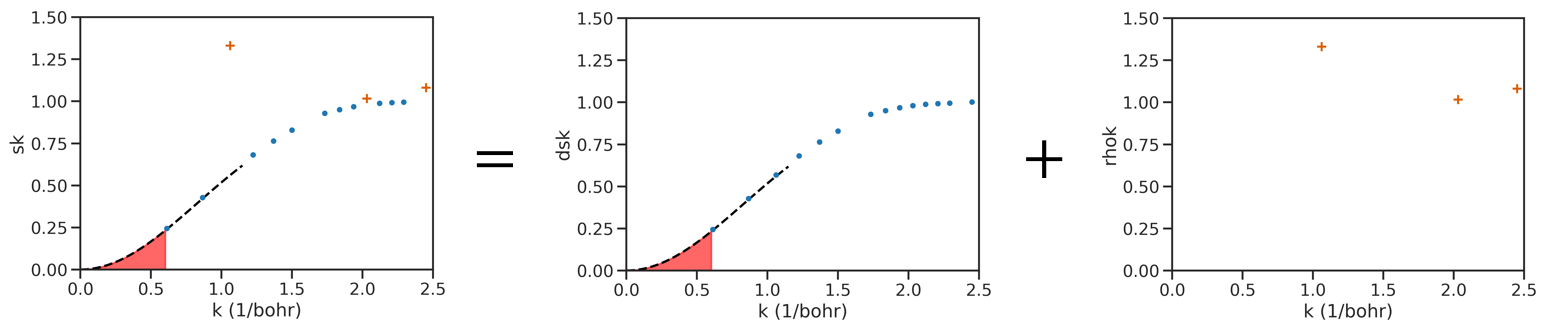
\includegraphics[width=\linewidth]{fsc-sk-dsk-rhok}
\caption{Fluctuating and static contributions from valence electrons in the conventional cell of bulk silicon.}
\label{fig:fsc-sk-dsk-rhok}
\end{figure}
As shown in Fig.~\ref{fig:fsc-sk-dsk-rhok}, the static part due to charge density $\rho_{\bs{k}}$ is non-zero only at reciprocal lattice of the primitive cell of the underlying crystal structure, whereas the fluctuating part varies smoothly from $0$ to $1$. Its value within the missing $\bs{k}=\bs{0}$ region (red area in Fig.~\ref{fig:fsc-sk-dsk-rhok}) can be used to correct the potential energy to leading order following eq.~(\ref{eq:fsc-dvn-missing}).
Changes in the charge density with system size is a higher-order effect and is small compared to the total potential energy~\cite{Clay2016}. However, as shown in Ref.~\cite{Yang2020-gap}, this static contribution becomes important when energy differences are taken, such as in the calculation of the fundamental gap.

Equation~(\ref{eq:wf-gaskell-rpa-sk}) still works well at $k\ll k_F$, but the short-range contribution $S_0(k)$ no longer comes from a simple determinant of plane waves. For insulators, dielectric screening suppresses long-range fluctuation and changes the leading-order behavior of $S(k)$ from eq.~(\ref{eq:wf-gaskell-rpa-sk-taylor}) to eq.~(7) in Ref.~\cite{Yang2020-gap}
\begin{align}
S(k) \approx \dfrac{k^2}{2\omega_p}(1-\epsilon_k^{-1})^{1/2},
\end{align}
so long as plasmons are the dominant excitation in the system.

\section{Correction to the kinetic energy}

\subsection{From momentum distribution}
The kinetic energy can be calculated as the second moment of the momentum distribution
\begin{align} \label{eq:fsc-tn-nk}
T_N \equiv T/N = \frac{1}{\rho}\int \dfrac{d^d\bs{k}}{(2\pi)^d} e(k) n_N(\bs{k}),
\end{align}
where the dispersion of non-relativistic particles
\begin{align}
e(k) = \dfrac{\hbar^2}{2m} k^2,
\end{align}
and $n_N(\bs{k})$ is the momentum distribution of these particles at the given system size $N$. It is crucial to distinguish the finite-size $n_N(\bs{k})$ from its thermodynamic limit $n_{\infty}(\bs{k})$, because it is a nonlocal quantity that converges slowly with system size~\cite{Holzmann2009}.
Similar to eq.~(\ref{eq:fsc-dvn}), the finite-size correction to the kinetic energy
\begin{align} \label{eq:fsc-dtn-nk}
\Delta T_N = \left[
\dfrac{1}{\rho}\int \dfrac{d^d\bs{k}}{(2\pi)^d} e(k)n_{\infty}(\bs{k})
\right] - \left[
\dfrac{1}{N}\sum\limits_{\bs{k}}
e(k)n_N(\bs{k})
\right].
\end{align}
The key difficulty in using eq.~(\ref{eq:fsc-dtn-nk}) is finding a reasonable approximation to $n_{\infty}(\bs{k})$. Some progress can be made by analyzing the Monte Carlo estimator for the Fourier transform of the momentum distribution, i.e. the off-diagonal one-particle density matrix~\cite{W.L.McMillan1965}
\begin{align} \label{eq:fsc-nr}
n(\bs{r}) = \left\langle \dfrac{\Psi(\bs{R}:\bs{r}_i\rightarrow\bs{r})}{\Psi(\bs{R})} \right\rangle_{\vert\Psi\vert^2},
\end{align}
where $\bs{R}$ denotes the positions of all $N$ particles, and the notation ``$:\bs{r}_i\rightarrow\bs{r}$'' means that particle $i$ is moved from $\bs{r}_i$ to $\bs{r}$.
As noted by W.R. Magro and D.M. Ceperley~\cite{Magro1994}, direct application of eq.~(\ref{eq:fsc-nr}) with periodic boundary condition can result in superfluous contributions, because all periodic images of particle $i$ are moved. The images will contribute to the ratio in eq.~(\ref{eq:fsc-nr}) if $\Psi$ has long-range components, e.g., eq.~(\ref{eq:fsc-rpa-wf}). Chiesa et al.~\cite{Chiesa2007} and Holzmann et al.~\cite{Holzmann2009} later used this observation to design a finite-size correction to the momentum distribution and the kinetic energy. To leading-order~\cite{Holzmann2009}
\begin{align} \label{eq:fsc-dnk-lo}
n_{\infty}(\bs{k}) - n_N(\bs{k}) \approx \int_{\frac{(2\pi)^d}{\Omega}}
\dfrac{d^d\bs{q}}{(2\pi)^d}
\left[
u_{\bs{q}}(1-S(\bs{q}))-\rho u(\bs{q})^2S(\bs{q})
\right]
\left(
n_N(\bs{k}+\bs{q})-n_N(\bs{k})
\right),
\end{align}
where $u_{\bs{q}}$ is the Jastrow pair potential in the wave function eq.~(\ref{eq:fsc-rpa-wf}).
As shown in Fig.~8 of Ref.~\cite{Yang2020-licp}, the leading-order correction to $n(\bs{k})$ works well for lithium. Further, Table~III in the Supplemental materials of Ref.~\cite{Yang2020-licp} shows that the corrected $n_N(\bs{k})$ can be used to accurately correct the finite-size error in the kinetic energy using eq.~(\ref{eq:fsc-dtn-nk}). To achieve this good result for a metal with a sharp Fermi surface such as lithium, it is crucial to densely sample momentum space while preserving the Fermi surface using grand-canonical twist averaging.

\subsection{From wave function}
Instead of using the relation between kinetic energy and the momentum distribution eq.~(\ref{eq:fsc-tn-nk}), one can directly analyze the QMC estimator for kinetic energy to find its finite-size correction. The VMC estimator for the kinetic energy of a Slater-Jastrow wave function $\Psi=De^{-U}$ is (from eq.~(14) of Ref.~\cite{Holzmann2016})
\begin{align} \label{eq:fsc-tn-vmc}
T_N^{VMC} = \frac{1}{N}\left\langle
-\sum\limits_{i=1}^N \dfrac{\hbar^2}{2m}\left[
\dfrac{\nabla_i^2D}{D} - (\bs{\nabla}_i U)^2
\right]
\right\rangle\equiv T_N^D + T_N^U.
\end{align}
The dominant finite-size correction in the determinant term is due to one-particle ``shell filling'' effects, whereas the dominant correction in the Jastrow term is due to long-range two-particle correlation. I will now discuss these two effects in turn.
\subsubsection{Single-particle ``shell filling'' effect}
If the orbitals in the determinant are from some effective one-particle theory such as HF or KS-DFT, then they are solutions of some effective one-particle potential $\veff$
\begin{align}
\left[
-\dfrac{\hbar^2\nabla^2}{2m} + \veff
\right] \phi_n(\bs{r}) = \epsilon_n\phi_n(\bs{r}).
\end{align}
Thus, one can work out the determinant contribution to the kinetic energy
\begin{align} \label{eq:fsc-tdn}
T^D_N \equiv -\dfrac{\hbar^2}{2m}\sum\limits_{i=1}^N \dfrac{\nabla_i^2D}{D} = \left[
\sum\limits_{n=1}^N\epsilon_n - \sum\limits_{i=1}^N \veff(\bs{r}_i)
\right],
\end{align}
by eq.~(19) in Ref.~\cite{Holzmann2016}. As the number of electrons is increased, the kinetic contribution eq.~(\ref{eq:fsc-tdn}) increases by the energies of the new orbitals being occupied. Consider the ideal Fermi gas in a 2D square box. As the number of same-spin particles increase from $N=2$ to $5$, the first shell of states in reciprocal space become filled. They all have the same single-particle energy, so the total kinetic energy increases linearly with $N$. However, when one adds a 6$^{\text{th}}$ particle, it increases the total energy by twice the amount as one in the first shell. As shown in Fig.~\ref{fig:fsc-lin-tabc}, this shell filling effect causes oscillation in the kinetic energy as a function of the number of particles, making size extrapolation difficult. This shell filling effect can be drastically reduced by adopting canonical twist averaged boundary conditions (TABC), where the number of particles is the same across all twists. Further, grand-canonical twist averaged boundary condition (GC-TABC), where the number of particles change to according to the exact Fermi surface, can exactly remove this single-particle finite-size effect. Finally, there is another ``pocket'' method which reduces the number of twists needed. Within a pocket in reciprocal space, the orbitals in the determinant smoothly acquire a phase as the twist is varied. Once these pockets are mapped out, one can perform one calculation per pocket and weigh it by the volume of the pocket to exactly remove the one-particle finite-size error~\cite{Holzmann2016}.

\begin{figure}[h]
\centering
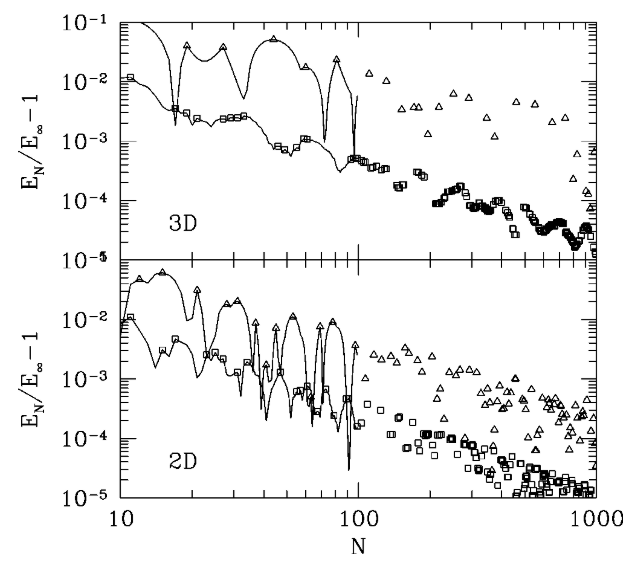
\includegraphics[width=0.6\linewidth]{lin-tabc}
\caption{Relative error of total energy vs. number of particles with PBC (up triangles) and TABC (squares) in 2D and 3D~\cite{Lin2001}}
\label{fig:fsc-lin-tabc}
\end{figure}

\subsubsection{Two-body size effect}
Using the RPA Jastrow pair potential from eq.~(\ref{eq:fsc-rpa-wf}), its contribution to eq.~(\ref{eq:fsc-tn-vmc}) becomes
\begin{align} \label{eq:fsc-tn-uk-sk}
T^U_N \equiv \dfrac{1}{N}\left\langle
\sum\limits_{i=1}^N \dfrac{\hbar^2}{2m} (\bs{\nabla}_iU)^2
\right\rangle
\approx \frac{1}{\Omega} \sum\limits_{\bs{k}\neq\bs{0}}
 \dfrac{\hbar^2}{2m} \rho u_{\bs{k}}u_{-\bs{k}}S(\bs{k}),
\end{align}
by eq.~(33) in Ref.~\cite{Holzmann2016}.
Recall the general relation between $S(\bs{k})$ and $u(\bs{k})$ eq.~(\ref{eq:uk-sk})
\begin{align}
2\rho u_{\bs{k}} \approx S^{-1}(\bs{k}) - S^{-1}_0(\bs{k}).
\end{align}
Since $S^{-1}(\bs{k})$ diverges faster than $S_0^{-1}(\bs{k})$ as $k\rightarrow0$, eventually $2\rho u_{\bs{k}} \approx S^{-1}(\bs{k})$. Thus, to leading-order eq.~(\ref{eq:fsc-tn-uk-sk}) becomes
\begin{align} \label{eq:fsc-tn-uk-ek}
T_N^U \approx \dfrac{1}{2\Omega} \sum\limits_{\bs{k}\neq\bs{0}}
e(k)u_{\bs{k}},
\end{align}
which should be compared with eq.~(\ref{eq:fsc-vn-vk}) for potential energy. Thus, the procedure to correct the two-body finite-size error in the kinetic energy is analogous to the potential correction scheme eq.~(\ref{eq:fsc-dvn})
\begin{align} \label{eq:fsc-dtn-uk}
\Delta T_N \equiv T_{\infty} - T_N = \left[
\int \dfrac{d^d\bs{k}}{(2\pi)^d} - \dfrac{1}{\Omega}\sum\limits_{\bs{k}}
\right] \frac{e(k)}{2} u(\bs{k}),
\end{align}
where $u(\bs{k})$ is an interpolation of the converged Jastrow pair potential, which can be approximated using the converged static structure factor in the long wavelength limit.

\subsubsection{Finite-temperature correction}
\textit{Based on notes from D. M. Ceperley}\\
At finite temperature and under the RPA, the long-range part of the action can be optimized to minimize the variance of the local energy, resulting in
\begin{align} \label{eq:fsc-finitet-uk}
2\rho u_k = Q(\bs{k}, \beta)^{-1}\tanh\left(
\dfrac{\beta}{2}\dfrac{e(k)}{Q(\bs{k}, \beta)}
\right) - S_0(\bs{k},\beta)^{-1},
\end{align}
where $\beta$ is inverse temperature, $e(k)=\lambda k^2$ is the dispersion of the particle, $\rho=N/\Omega$ is density, and $S_0(\bs{k}, \beta)$ is the non-interacting structure factors.
\begin{align}
Q(\bs{k}, \beta) \equiv \left(S_0(\bs{k}, \beta)^{-2}+\dfrac{2\rho v_{\bs{k}}}{e(k)}\right)^{-1/2}.
\end{align}
$Q(\bs{k}, \beta)$ reduces to Gaskell RPA $S(\bs{k})$ as $\beta\rightarrow\infty$. Since $\lim\limits_{x\rightarrow\infty}\tanh(x)=1$, eq.~(\ref{eq:fsc-finitet-uk}) becomes eq.~(\ref{eq:uk-sk}) in this limit. Assuming the relation between $S(\bs{k})$ and $u_{\bs{k}}$ eq.~(\ref{eq:uk-sk}) holds, the finite-temperature RPA structure factor is
\begin{align} \label{eq:fsc-finitet-sk}
S(\bs{k},\beta) = Q(\bs{k},\beta)/\tanh\left(
\dfrac{\beta}{2}\dfrac{e(k)}{Q(\bs{k}, \beta)}
\right).
\end{align}
Equations~(\ref{eq:fsc-finitet-uk}) and (\ref{eq:fsc-finitet-sk}) can be used to derived leading-order finite-size corrections to the kinetic and potential energies using eq.~(\ref{eq:fsc-dtn-uk}) and (\ref{eq:fsc-dvn}), respectively.

\begin{comment}
\section{Overview}
How does finite size error scale with system size?

What are typical methods used to deal with finite-size error?
1. extrapolation based on Fermi-liquid theory. For bosons?
2. rely on effective one-particle theory e.g. HF and DFT.
3. two-body finite-size correction

\section{Periodic boundary condition (PBC)}
There are two types of finite-size errors in simulations with periodic boundary condition. The first is the artificial correlation between periodic images.

% Fermi liquid

% Chiesa

% MPC

% KZK

\section{Thermodynamic limit}
The key quantity to consider in QMC is the local energy
\begin{align}
E_L = -\sum\limits_i \lambda_i \left[
\dfrac{\nabla_i^2D}{D} - (\nabla_iU)^2 - \nabla_iU\nabla_i(U_{FN}-U)
\right] + V.
\end{align}

\subsection{Shell-filling effect}
\subsection{Electronic structure factor $S(k)$}
\subsection{Jastrow pair function $U(k)$}
\subsection{Electronic momentum distribution $n(k)$}
\section{Grand-canonical twist-averaged boundary condition (GC-TABC)}
\end{comment}

%\chapter{Benchmark of dynamic-ion QMC on small molecules}
This chapter is based on the following article(s):

\textit{I}. Yubo Yang, Ilkka Kyl\"anp\"a\"a, Norm Tubman, Jaron Krogel, Sharon Hammes-Schiffer, and David Ceperley, ``How large are nonadiabatic effects in atomic and diatomic systems?" J. Chem. Phys. \textbf{143}, 124308 (2015).

\textit{II}. Norm Tubman, Yubo Yang, Sharon Hammes-Schiffer, and David Ceperley, ``Interpolated wave functions for nonadiabatic simulations with the fixed-node quantum Monte Carlo method," ACS Symp. Ser. \textbf{1234}, pp. 47-61 (2016).

\section{Introduction}
There have been several recent discoveries~\cite{Tubman_ECG,cederbaum1,gross2014,boent,Martinez_Review} suggesting that quantum wave functions, which include both electronic and ionic degrees of freedom, have many interesting properties that have yet to be explored.  This includes the development of equations that exactly factorize a wave function into electronic and ionic components,~\cite{cederbaum1,cederbaum12} the disappearance of conical intersections in wave functions of model systems,~\cite{gross2014} and the use of quantum entanglement to study electronic and ionic density matrices.~\cite{boent} Extending such studies to realistic systems is of broad interest and will considerably expand our understanding of electron-ion systems. However, treatment of \textit{ab initio} electron-ion systems is challenging, and applications have thus been limited. The most accurate simulations of electron-ion wave functions are generally done with very specialized wave functions, which are limited to rather small systems.~\cite{mitroy2013} Methods are also being developed to treat larger systems with different regimes of validity.~\cite{Sharon_NEO-HF,Sharon_XCNEO-HF1,Sharon_XCNEO-HF2,Sharon_XCNEO-HF,Kurt_XCNEO-HF,Kurt_XCNEO-HF1,Sharon_NEO-DFT,Sharon_NEO-DFT2,Sharon_NEO-DFT3,Gross_NEO-DFT,Gross_NEO-DFT1,Ilkka_Path,Ilkka_Path1,Ilkka_Path2}

As a framework to address these problems in general realistic systems, we recently demonstrated that quantum Monte Carlo (QMC) can be combined with quantum chemistry techniques to generate electron-ion wave functions.~\cite{Tubman_ECG} We treated realistic molecular systems and demonstrated that our method can be scaled to larger systems than previously considered while maintaining a highly accurate wave function. In the following, we extend our previous work by considering the simulation of a larger set of atoms and molecules. We calculate ionization energies and atomization energies that can be directly compared with previous results for benchmarking purposes.

\section{Method}
\subsection{Fixed-Node Diffusion Monte Carlo (FN-DMC)}
Diffusion Monte Carlo~\cite{Anderson_DMC,lester1,Stuart_Review,Needs_Review,Needs_Old_Review,QMC_Review} is a projector method that evolves a trial wave function in imaginary time and projects out the ground-state wave function. For practical simulations of fermions, the fixed-node approximation is introduced, which depends only on the set of electronic positions where a trial wave function is equal to zero.  This approximation is different than approximations typically used in quantum chemistry calculations. In this work, we demonstrate that we can generate high-quality nodal surfaces for a range of systems that include full electron-ion wave functions. 

If the trial wave function has the same nodal surface as the exact ground-state wave function, FN-DMC will obtain the exact ground-state energy.  Approximate nodal surfaces can be generated through optimization of the full wave function. Such approximate nodal surfaces have been tested and validated on a wide range of systems, and consistently provide an excellent approximation of the exact ground-state energy, comparable to the state of the art in \textit{ab initio} simulations.~\cite{grossman1} In addition, the energies generated with FN-DMC are variational with respect to the ground-state energy.

In all but a handful of previous QMC simulations,~\cite{Ceperley_1987,Natoli_1993,Natoli_1995,Chen_1995,Coldwell_H2_2008,Gabriele_H2_2004,Sandro_finiteT-noBO_2012} calculations are performed with nuclei ``clamped" to their equilibrium positions. However, such an assumption is not fundamentally required by FN-DMC. %In our previous work we find that the most important effects for optimizing are the nodes due to electron-electron correlation~\cite{Tubman_ECG}, and in this regard we use more sophisticated terms in the electronic part of the wave function than in the ionic part.

\subsection{Electronic Wave Function and Optimization}

There are several different approaches for generating electronic wave functions for a FN-DMC calculation.~\cite{Umrigar_Alleviation,Toulouse_Bench,Brown_Bench,Seth_Bench} Recent advances~\cite{Nightingale_Linear,Umrigar_Linear,Brown_Bench} have made it possible to simultaneously optimize thousands of wave function parameters using variational Monte Carlo with clamped nuclei. We use an initial guess for the wave function that is generated from complete active space self-consistent-field (CASSCF)~\cite{Chaban_MCSCF,Szabo} calculations using the quantum chemistry package GAMESS-US.~\cite{GAMESS} The optimized orbitals are then used in a configuration interaction singles and doubles (CISD) calculation to generate a series of configuration state functions (CSFs).~\cite{Pauncz_CSF} For the small systems Li$^+$, Be$^+$, LiH and BeH, a CASSCF calculation with a large active space is used in place of CISD. The multi-CSF expansion of the wave function can be expressed in the following form,
\begin{align}
\Psi_{\text{CISD}}(\vec{r};\vec{R}_o)=\sum\limits_{i=1}^{N_{\text{CSF}}}\alpha_i\phi_i(\vec{r};\vec{R}_o), \label{eq:psi_gms}
\end{align}
where $\vec{r}$ refers to the spatial coordinates of all the electrons and $\vec{R}_o$ refers to the equilibrium positions of all the ions. $\phi_i(\vec{r})$ and $\vec{\alpha}=\{\alpha_1,\alpha_2,\dots\}$ are the CSFs and CI coefficients generated from CISD. The cc-pV5Z basis~\cite{dunning} is used for the atomic systems and the Roos Augmented Triple Zeta ANO basis~\cite{roos} is used for the molecular systems except for the smallest system LiH, where the cc-pV5Z basis is used.

After the multi-CSF expansion is generated, we impose the electron-nucleus cusp condition on each molecular orbital~\cite{cusp} and add a Jastrow factor to the wave function to include electron correlation.~\cite{Kato} Our Jastrow factor contains electron-electron, electron-nucleus and electron-electron-nucleus terms. The full electronic wave function used in FN-DMC is,
\begin{align}
\psi_e(\vec{r};\vec{R})=e^{J(\vec{r},\vec{R},\vec{\beta})}\Psi_{\text{CISD}}(\vec{r};\vec{R})\label{eq:psie}.
\end{align}
We optimize the CSF and Jastrow coefficients, $\vec{\alpha}$ and $\vec{\beta}$, respectively, simultaneously with QMCPACK.~\cite{QMCPACK_Kim,QMCPACK_Esler} Optimization is performed with the ions clamped to their equilibrium positions $\vec{R}_o$. The equilibrium geometries for BeH and BH are chosen to be the ECG-optimized distances for comparison with the ECG (explicitly correlated Gaussian) method, and the geometries for the rest of the hydrides are taken from experimental data\cite{CCCBDB}. We use 3.015 a.u. as the equilibrium inter-nuclei distance for LiH, as this geometry is found to provide a lower clamped-nuclei ground-state energy than the ECG optimized distance of 3.061 a.u.. We include all CSFs with coefficients larger than a specific cutoff $\epsilon$ to lend reasonable flexibility to the wave function during optimization. We include as many CSFs as possible to maximize the flexibility of the wave function. However, the inclusion of too many CSFs with small expansion coefficients can introduce noise as they require a large number of samples in the optimization step to be optimized. We have chosen $\epsilon$ to restrict the number of CSFs in the wave function to be $\sim$1000 in all systems studied. Optimization is performed with the linear method~\cite{Umrigar_Linear} with roughly $10^6$ statistically independent samples.%, and we use a cost function consisting a linear combination of average local energy and reweighted variance.

%The specific choices of active space for the systems studied are listed in Table \ref{tab:CAS}.
%\input{Table/cas}

\begin{figure}[h]
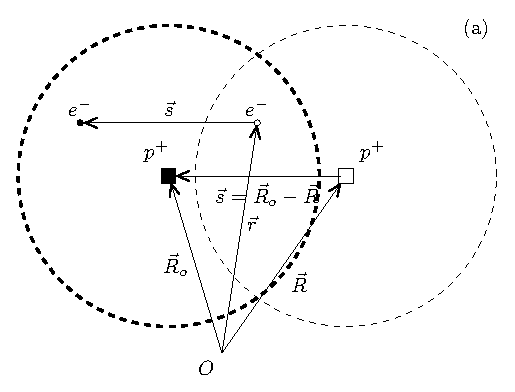
\includegraphics[width=0.49\textwidth]{fig1a}
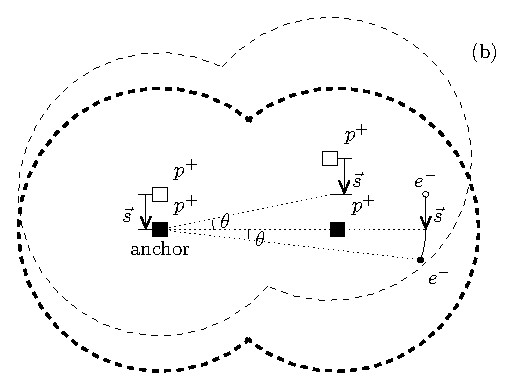
\includegraphics[width=0.49\textwidth]{fig1b}
\caption{Dragged-node approach for simulation of atomic and molecular systems in QMC. {\bf (a)} For atomic systems we can consider the entire wave function shifting with the ion. This process can be visualized by following a contour of the wave function. The thick dashed circle represents a contour of the electronic wave function when the proton is at its reference position $\vec{R}_o$, and the thin dashed circle represents the same contour when the proton has moved to a new position $\vec{R}$. To evaluate the ion-dependent electronic wave function $\bar{\psi}_e(\vec{r},\vec{R})$, we simply map the electron to its proper place in the reference wave function $\psi_e(\vec{r};\vec{R}_o)$. That is, $\bar{\psi}_e(\vec{r},\vec{R})=\bar{\psi}_e(\vec{r}+\vec{s},\vec{R}_o)=\psi_e(\vec{r}+\vec{s};\vec{R}_o)$ where $\vec{s}$ is the shift required to put the proton back to its reference position. {\bf (b)} For H$_2^+$, we pick one of the protons as an ``anchor'' and approximate the new wave function by dragging the reference wave function with the ``anchor'' proton. We also rotate the wave function to align its axis of symmetry with the orientation of the two protons. \label{fig:drag}}
\end{figure}

\subsection{Electron-Ion Wave Function}

Once a satisfactory electronic wave function has been obtained, we construct the electron-ion wave function using the ansatz,
\begin{align}
\Psi_{eI}(\vec{r},\vec{R})=\psi_I(\vec{R})\bar{\psi}_e(\vec{r},\vec{R}), \label{eq:psi}
\end{align}
where $\vec{R}$ denotes the spatial coordinates of all ions and $\bar{\psi}_e(\vec{r},\vec{R})$ is an ion-dependent electronic wave function adapted from the clamped-nuclei wave function $\psi_e(\vec{r};\vec{R}_o)$ through basis set dependence. Due to the localization of Gaussian basis sets around nuclei, as used in quantum chemistry calculations, the nodes of $\bar{\psi}_e$ change based on the ionic positions, which we have previously called the dragged-node approximation.~\cite{Tubman_ECG}
%In general, the nodes only coincide with those obtained in the clamped-ion limit when the ions are at their equilibrium positions $\bar{\psi}_e(\vec{r},\vec{R}_o)=\psi_e(\vec{r};\vec{R}_o)$. However, for atoms and ions this approximation is equivalent to re-optimizing the electronic wave function at each ionic configuration, i.e. $\bar{\psi}_e(\vec{r},\vec{R})=\psi_e(\vec{r};\vec{R})$. 
Although there are approaches for going beyond the dragged-node approximation, it was demonstrated to be highly accurate over a range of molecules in previous work.~\cite{Tubman_ECG} For the systems considered here, we can impose various symmetries of the Hamiltonian onto the wave function that arise from the relative motion of the ions. In Fig.~\ref{fig:drag} we demonstrate this approach for the simple cases of a hydrogen atom and an H$_2^+$ molecular ion. This approach can be generalized for use in larger systems or even applied to parts of a bigger system, e.g., treating light ions as quantum particles and heavy ions as ``clamped".

The term $\psi_I$ consists of simple products of Gaussian wave functions over each pair of nuclei,
\begin{align}
\psi_I(\vec{R})\propto \prod\limits_{i,j>i}e^{-a_{ij}(\vert \vec{R}_i-\vec{R}_j\vert-b_{ij})^2},
\label{wfs_ions}
\end{align}
where $a_{ij}$ is a coefficient that is optimized and $b_{ij}$ are taken to be the equilibrium distances between the nuclei. Since $\psi_I$ is nodeless, the choice of the variational parameters $a_{ij}$ and $b_{ij}$ does not affect the converged FN-DMC energy. FN-DMC is then performed with the fully optimized electron-ion wave function. We perform timestep extrapolation for all of the tested systems. At least four timesteps from $0.005~\text{Ha}^{-1}$ to $0.0005~\text{Ha}^{-1}$ are used for all systems studied in the clamped-nuclei FN-DMC calculation, and at least three timesteps from $0.005~\text{Ha}^{-1}$ to $0.0001~\text{Ha}^{-1}$ are used in the nonadiabatic FN-DMC calculation.

Using definitions from Ref.~\cite{Cederbaum_Review}, the adiabatic approximation will refer to the complete neglect of the nonadiabatic coupling matrix when the Schr$\ddot{\text{o}}$dinger equation is expressed in the basis of eigenstates of the electronic Hamiltonian. In this context, the nonadiabatic contribution to an eigenvalue of the electronic Hamiltonian can be partitioned into two parts: the diagonal Born-Oppenheimer correction (DBOC), which involves only the single electronic state of interest, and the remaining corrections arising from terms that involve excited eigenstates of the electronic Hamiltonian. The DBOC discussed in this work is the expectation value of the nuclear kinetic energy operator in the ground adiabatic electronic state. We define the clamped-nuclei ground-state energy $E_c$ as the lowest eigenvalue of the electronic Hamiltonian and the nonadiabatic ground-state energy $E_n$ as the lowest eigenvalue of the full molecular Hamiltonian that includes the nuclear kinetic energy operator. The zero-point energy (ZPE) for a diatomic molecule is the energy of the ground vibrational state of the one-dimensional vibrational mode. Note that the ZPE of the nuclei is part of the difference $E_n-E_c$. The ZPE is not considered to be nonadiabatic, but its contribution is included in the full molecular Hamiltonian.

\section{Results and Discussion}
\begin{table*}[t!]
\setlength{\extrarowheight}{1pt}
\begin{threeparttable}

\caption{Ground-state energies for atoms and ions and the ionization energies for the atoms:  fixed-node DMC results of this work (FN-DMC) for atoms and ions with and without the Born-Oppenheimer approximation. The rows marked with bold \textbf{FN-DMC} are our nonadiabatic results. The ionization potentials (IPs) are reported in the last section of the table. Energies are given in units of Hartree. For the highly accurate Hylleraas and ECG results, up to 8 digits are reported in the table. \label{tab:ionization}}
\small
\begin{tabular}
% siunitx setup
{
 l
 S[table-format=1.6]
 S[table-format=5.6]
 S[table-format=5.6]
 S[table-format=4.6]
 S[table-format=4.6]
 S[table-format=4.6]
 S[table-format=4.6]
 S[table-format=4.6]
}

\hline\hline
\multicolumn{1}{c}{Atom} & 
\multicolumn{1}{c}{Li$(^2$S)} &
\multicolumn{1}{c}{Be$(^1$S)} &
\multicolumn{1}{c}{B$(^2$P)} &
\multicolumn{1}{c}{C$(^3$P)} &
\multicolumn{1}{c}{N$(^4$S)} &
\multicolumn{1}{c}{O$(^3$P)} &
\multicolumn{1}{c}{F$(^2$P)} \\ 
\hline
\multicolumn{1}{c}{} & 
\multicolumn{1}{c}{} &
\multicolumn{1}{c}{} &
\multicolumn{1}{c}{clamped-ion} &
\multicolumn{1}{c}{} &
\multicolumn{1}{c}{} &
\multicolumn{1}{c}{} &
\multicolumn{1}{c}{} \\
FN-DMC & \text{-}7.478057(5) & \text{-}14.66731(1) & \text{-}24.65374(2) & \text{-}37.84448(2) & \text{-}54.58851(6) & \text{-}75.0658(2) & \text{-}99.73177(6) \\
Seth DMC \cite{Seth_Bench} & \text{-}7.478067(5) & \text{-}14.667306(7) & \text{-}24.65379(3) & \text{-}37.84446(6) & \text{-}54.58867(8) & \text{-}75.0654(1) & \text{-}99.7318(1) \\
$E_{\text{ref}}$\tnote{a} &  \text{-}7.4780603 & \text{-}14.667356 & \text{-}24.653866 & \text{-}37.8450 & \text{-}54.5892 & \text{-}75.0673 & \text{-}99.7339 \\
\multicolumn{1}{c}{} & 
\multicolumn{1}{c}{} &
\multicolumn{1}{c}{} &
\multicolumn{1}{c}{nonadiabatic} &
\multicolumn{1}{c}{} &
\multicolumn{1}{c}{} &
\multicolumn{1}{c}{} &
\multicolumn{1}{c}{} \\
\textbf{FN-DMC} & \text{-}7.47742(2) & \text{-}14.66643(3) & \text{-}24.65252(4) & \text{-}37.84273(4) & \text{-}54.58641(5) & \text{-}75.06313(6) & \text{-}99.7293(1) \\
ECG \tnote{b} & \text{-}7.4774519 & \text{-}14.666435 & \text{-}24.652624 & \text{-}37.841621 & N/A & N/A & N/A \\
\hline

\multicolumn{1}{c}{Ion} & 
\multicolumn{1}{c}{$\text{Li}^+(^1$S)} &
\multicolumn{1}{c}{$\text{Be}^+(^2$S)} &
\multicolumn{1}{c}{$\text{B}^+(^1$S)} &
\multicolumn{1}{c}{$\text{C}^+(^2$P)} &
\multicolumn{1}{c}{$\text{N}^+(^4$S)} &
\multicolumn{1}{c}{$\text{O}^+(^3$P)} &
\multicolumn{1}{c}{$\text{F}^+(^2$P)} \\ 
\hline
\multicolumn{1}{c}{} & 
\multicolumn{1}{c}{} &
\multicolumn{1}{c}{} &
\multicolumn{1}{c}{clamped-ion} &
\multicolumn{1}{c}{} &
\multicolumn{1}{c}{} &
\multicolumn{1}{c}{} &
\multicolumn{1}{c}{} \\
FN-DMC & \text{-}7.27989(2) & \text{-}14.324749(7) & \text{-}24.34883(1) & \text{-}37.43071(2) & \text{-}54.05371(5) & \text{-}74.56597(6) & \text{-}99.0909(1) \\
Seth DMC \cite{Seth_Bench} & \text{-}7.279914(3) & \text{-}14.324761(3) & \text{-}24.34887(2) & \text{-}37.43073(4) & \text{-}54.05383(7) & \text{-}74.56662(7) & \text{-}99.0911(2) \\
$E_{\text{ref}}$\tnote{c} & \text{-}7.2799134 & \text{-}14.324763 & \text{-}24.348884 & \text{-}37.430880 & \text{-}54.0546 & \text{-}74.5668 & \text{-}99.0928 \\ 
\multicolumn{1}{c}{} &
\multicolumn{1}{c}{} &
\multicolumn{1}{c}{} &
\multicolumn{1}{c}{nonadiabatic} &
\multicolumn{1}{c}{} &
\multicolumn{1}{c}{} &
\multicolumn{1}{c}{} &
\multicolumn{1}{c}{} \\
\textbf{FN-DMC} & \text{-}7.27931(4) & \text{-}14.32387(2) & \text{-}24.34758(3) & \text{-}37.42899(6) & \text{-}54.05165(4) & \text{-}74.5634(1) & \text{-}99.0885(1) \\
ECG \tnote{d} & N/A &  \text{-}14.323863 &  \text{-}24.347641 &  \text{-}37.429169 & N/A & N/A & N/A \\
\hline
\multicolumn{1}{c}{} & 
\multicolumn{1}{c}{} &
\multicolumn{1}{c}{} &
\multicolumn{1}{c}{clamped-ion} &
\multicolumn{1}{c}{} &
\multicolumn{1}{c}{} &
\multicolumn{1}{c}{} &
\multicolumn{1}{c}{} \\
IP (FN-DMC) & 0.19817(2) & 0.34256(1) & 0.30490(2) & 0.41377(3) & 0.53479(8) & 0.4998(2) & 0.6409(1) \\
\multicolumn{1}{c}{} & 
\multicolumn{1}{c}{} &
\multicolumn{1}{c}{} &
\multicolumn{1}{c}{nonadiabatic} &
\multicolumn{1}{c}{} &
\multicolumn{1}{c}{} &
\multicolumn{1}{c}{} &
\multicolumn{1}{c}{} \\
IP (\textbf{FN-DMC}) & 0.19811(4) & 0.34257(4) & 0.30494(5) & 0.41374(7) & 0.53476(7) & 0.4998(1) & 0.6408(1) \\
IP (Ref.)\tnote{e} & 0.198130 & 0.342572 & 0.304980 & 0.414014 & 0.534775 & 0.500452 & 0.640946 \\
\hline\hline
\end{tabular}

\begin{tablenotes}
\item[a] For the atomic references, we use the Hylleraas result for Li,~\cite{Wang_Li} and ECG results for Be~\cite{Stanke_Be} and B.~\cite{Bubin_B} Ref.~\cite{Davidson_Atoms} is used for C,N,O and F where the ground-state energies are taken from Table XI.
\item[b] We use nonadiabatic ECG results as the reference for Li,~\cite{Stanke_Li} Be~\cite{Bubin_BeH_noBO} and B~\cite{Bubin_B}, which are converged to the true ground-state to well within 0.1 mHa. The result for C,~\cite{Bubin_C} however, may have error on the order of 1 mHa.
\item[c] For the ionic references, we use the ICI result for $\text{Li}^+$,~\cite{Nakashima_Li+} Hylleraas result for $\text{Be}^+$~\cite{Puchalski_Be} and ECG results for $\text{B}^+$~\cite{Bubin_B+} and $\text{C}^+$.~\cite{Bubin_C+,mitroy2013} Ref.~\cite{Davidson_Atoms} is used for $\text{N}^+$,$\text{O}^+$,$\text{F}^+$.
\item[d] ECG references only exist for $\text{Be}^+$,~\cite{Bubin_BeH_noBO} $\text{B}^+$~\cite{Bubin_B+} and $\text{C}^+$.~\cite{Bubin_C+}
\item[e] Spin-orbit coupling and relativistic corrections~\cite{Klopper_IP} are removed from experimental data~\cite{NIST_Atoms} for comparison.
\end{tablenotes}

\end{threeparttable}
\end{table*}

\subsection{Atoms and Ions}

To assess the quality of our results for atoms and ions~\footnotemark\footnotetext{All calculations are performed for the most abundant isotope. In units of electron mass, the isotope masses for Li, Be, B, C, N, O, F are taken to be 12782.4327, 16419.2608, 20214.7648
6, 21862.7553, 25512.1484, 29141.0754, 34613.1200, respectively. The Li mass used for the LiH molecule is 12649.6690, which is slightly different from that used for the atomic Li simulations, but we do not expect this to affect our results within our statistical errors.}, we compare to previous results from highly accurate simulations, as presented in Table \ref{tab:ionization}. For the clamped-ion results, QMC~\cite{Brown_Bench,Toulouse_Bench,Seth_Bench,Morale_Bench,Rappe_Bench} and quantum chemistry benchmarks are available for comparison. To illustrate the high-quality QMC techniques used in this work, we compare our clamped-ion atomic results with a recent QMC benchmark study.~\cite{Seth_Bench} The ground-state FN-DMC energies consistently agree across all systems studied (except for O$^{+}$) within 0.1 mHa. This shows that similar nodes can be obtained with different forms of the wave function. In particular, our large ($\sim$ 1000 CSF) multi-determinant expansions can be compared with the approach used by Seth {\it et al.},~\cite{Seth_Bench} which relies on moderately-sized multi-determinant expansions ($\sim$ 100 CSF) with a backflow transformation. For certain atoms, we can compare to more accurate simulation techniques. For C$^+$ as well as the neutral and ionized Li, Be and B, well-converged ECG calculations are available, where basis set error is converged to less than 0.1 mHa. This convergence is corroborated by results from the Hylleraas method for Li~\cite{Wang_Li} and Be$^+$.~\cite{Puchalski_Be} In Table \ref{tab:ionization}, we have used the lowest variational results as our references for these systems, as the convergence is such that the accuracy is higher than other current theoretical or experimental estimates. 

All of our clamped-ion results agree within 0.2 mHa of the ECG references, as shown in Figure \ref{fig:atom-ECG}. The error bars for the reference ECG results are absorbed into the DMC error bars for clarity, because the ECG error bars are orders of magnitude smaller compared to the DMC error bars. While ECG results exist for C and N, they are not well converged and are not suitable references.~\cite{Bubin_C,Sharkey_N} The benchmark results in Ref.~\cite{Davidson_Atoms} are a standard for atomic energies, and we report them as our references in Table \ref{tab:ionization} for the larger atoms. However, these benchmark results are not consistently accurate to 0.1 mHa. For instance, if we use the ECG results for $\text{C}^+$ with the most accurate ionization reference energy, then we find a reference energy for the C atom of -37.84489 Ha, which is 0.1 mHa higher than that reported in Ref.~\cite{Davidson_Atoms}. %Nevertheless, a comparison of our results with the references suggests that our ground-state energies for the neutral and ionized N,O,F are not accurate to the sub mHa level. 
The systems with the most error are O and F, for which other QMC studies seem to experience similar difficulties.~\cite{Seth_Bench,Booth_FCIQMC,Brown_Bench,Shiwei_AFQMC} We note that for some of these systems it may be possible to absorb the sign problem and increase the accuracy further in future studies.~\cite{Tubman_Release,Tubman_ACS} %However, a systematic exploration of these alternatives is beyond the scope of the current study.

\begin{figure}[h]
\centering
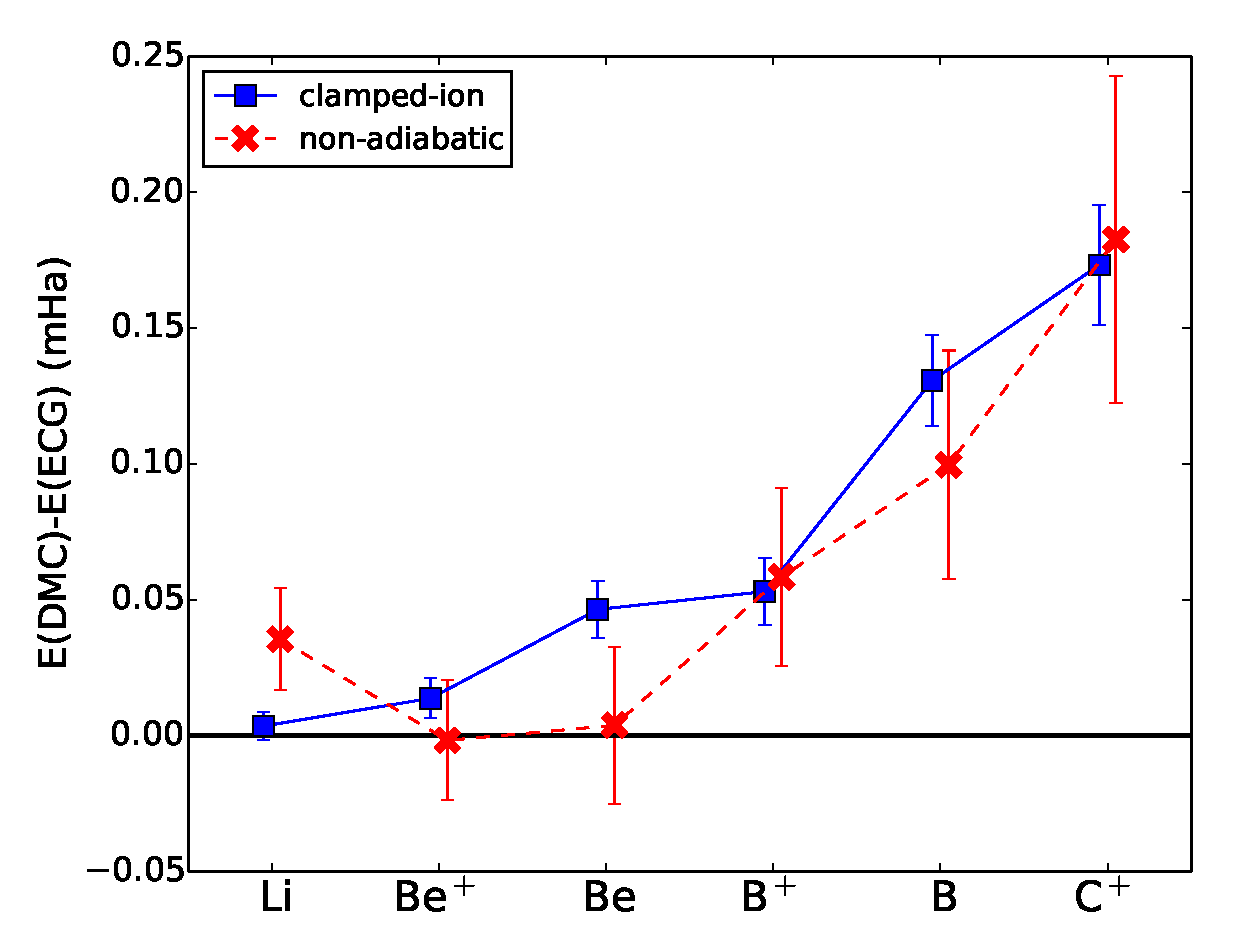
\includegraphics[width=0.8\textwidth]{atom-ECG}
\caption{FN-DMC ground state energies for $\text{Be}^+$, Be, $\text{B}^+$, B, $\text{C}^+$ relative to ECG references~\cite{Stanke_Be,Puchalski_Be,Bubin_BeH_noBO,Bubin_B,Bubin_B+,Bubin_C+} for either clamped-ion or nonadiabatic calculations. These relative energies provide an estimate for the fixed-node error in the electronic and electron-ion wave functions, respectively.\label{fig:atom-ECG}}
\end{figure}

It is more difficult to find accurate references for the nonadiabatic results. We provide the first nonadiabatic QMC benchmarks for the first-row atoms. There are six ECG calculations of nonadiabatic ground-state energies that are reportedly converged beyond 0.1 mHa, which we use as references. Our reported nonadiabatic ground-state energies for Li, Be, $\text{Be}^+$, B, $\text{B}^+$ and $\text{C}^+$ are in agreement with the ECG results to within 0.2 mHa, as shown in Figure \ref{fig:atom-ECG}. For these systems, the ECG results are converged to essentially the exact ground-state energies in both the clamped-ion and nonadiabatic cases. The difference between our DMC ground-state and ECG reference is the fixed-node error present in our wave functions. We would expect the clamped ion results to be more accurate than the nonadiabatic results, since the nonadiabatic wave functions are inherently more difficult to construct.  However, for the systems in Figure \ref{fig:atom-ECG}, this difference in quality is less than 0.1 mHa.
%In the case of Be, $\text{Be}^+$, and B,  the nonadiabatic wave function is actually more accurate than the corresponding clamped-ion wave function.

No reference calculations exist for the heavier atoms N, O, and F. However, it is possible to apply finite-mass correction~\cite{Davidson_Atoms,Cencek_LiH} (i.e., divide by $1+m_e/M$, where $m_e$ is the mass of an electron and $M$ is the mass of the nucleus) to the best clamped-ion references to estimate the nonadiabatic references. The energies for N, O, and F obtained in this way are -54.5871, -75.0647 and -99.7310 Ha, respectively. For the ionized states, we obtain -54.0525, -74.5643 and -99.0900 Ha. %A comparison of our results to these references reveals that the electronic and electron-ion wave functions are of similar quality for all atoms and ions. %Notice the fixed-node error is virtually identical in the electronic wave function and electron-ion wave function of the same system, suggesting that our approach is capable of generating high quality electron-ion wave function from an optimized electronic wave function.

\begin{figure}[h]
\centering
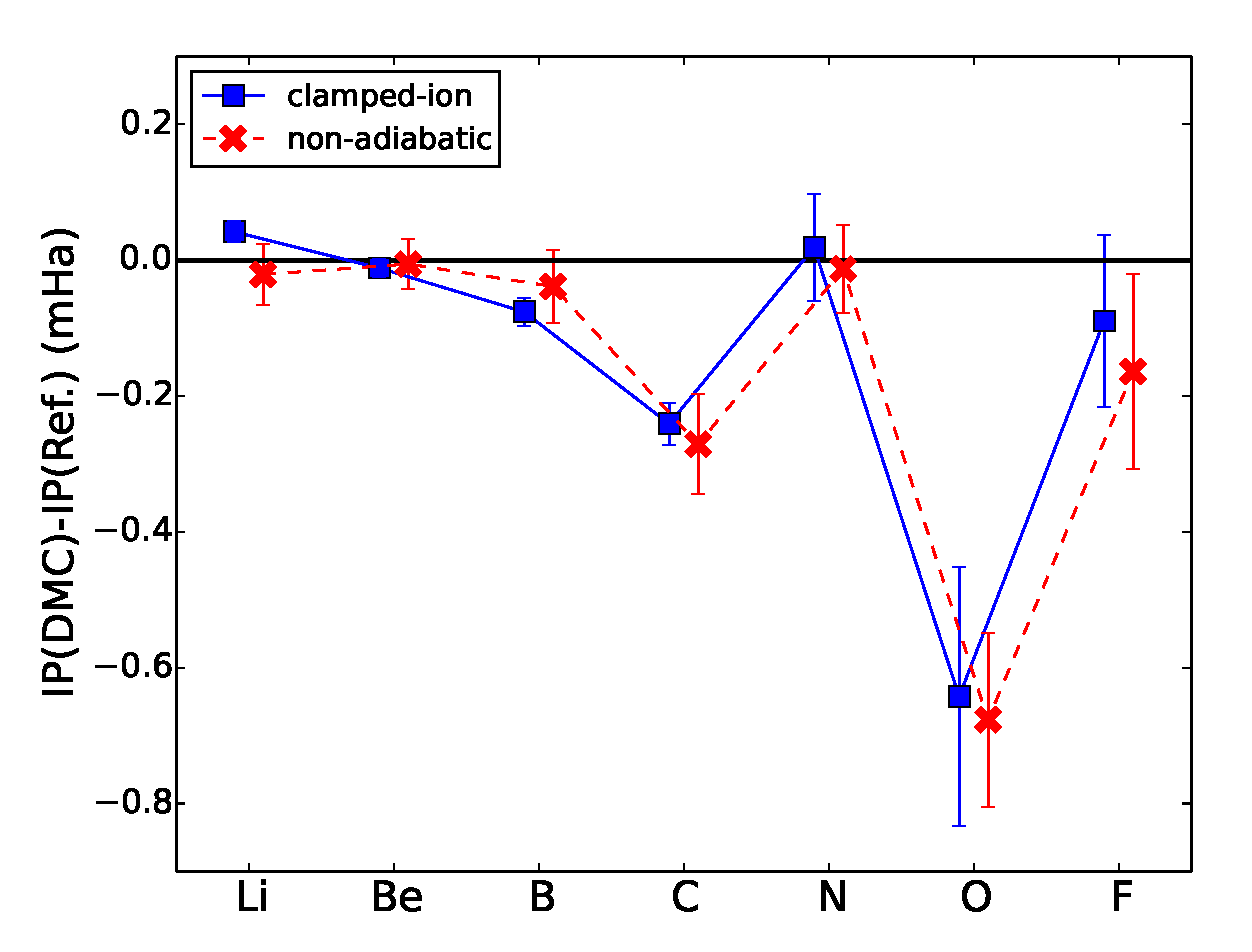
\includegraphics[width=0.8\textwidth]{ionization}
\caption{Calculated ionization energies relative to reference data. The same reference is used for both clamped-ion and nonadiabatic results. The calculated energies are all within 1 mHa of the reference. \label{fig:ionization}}
\end{figure}

The ionization potentials are reported in Table \ref{tab:ionization} and shown in Figure \ref{fig:ionization}. For determining a set of nonadiabatic reference data, we subtract the spin-orbit and relativistic corrections (estimated by Klopper et. al.~\cite{Klopper_IP}) from the NIST experimental data.~\cite{NIST_Atoms} Ref.~\cite{Klopper_IP} is considered to have the most accurate ionization energies due to its usage of state-of-the-art quantum chemistry techniques shown to provide close agreement with experiment.
%We believe these are more accurate than another widely used reference~\cite{Davidson_Atoms} because the latter estimates ionization potentials in the infinite-nucleus-mass limit, and the former uses corrections from state-of-the-art quantum chemistry techniques. However, the differences between the two references are only significant for obtaining benchmarks better than 0.5 mHa. 
For the atoms considered in this work, ionization energies have previously been predicted to be independent of all nonadiabatic effects beyond the DBOC to within an accuracy of 0.1 mHa.~\cite{Klopper_IP} This prediction is based on calculations that are reported to be exact and agree to high accuracy with experiment. As shown in Figure \ref{fig:ionization}, the ionization potentials calculated with and without the Born-Oppenheimer approximation are all within 1 mHa of the reference energies. Further, the clamped-ion and nonadiabatic predictions for the ionization potentials are statistically indistinguishable for all systems studied, consistent with the previous study.~\cite{Klopper_IP}

\begin{figure}[h]
\centering
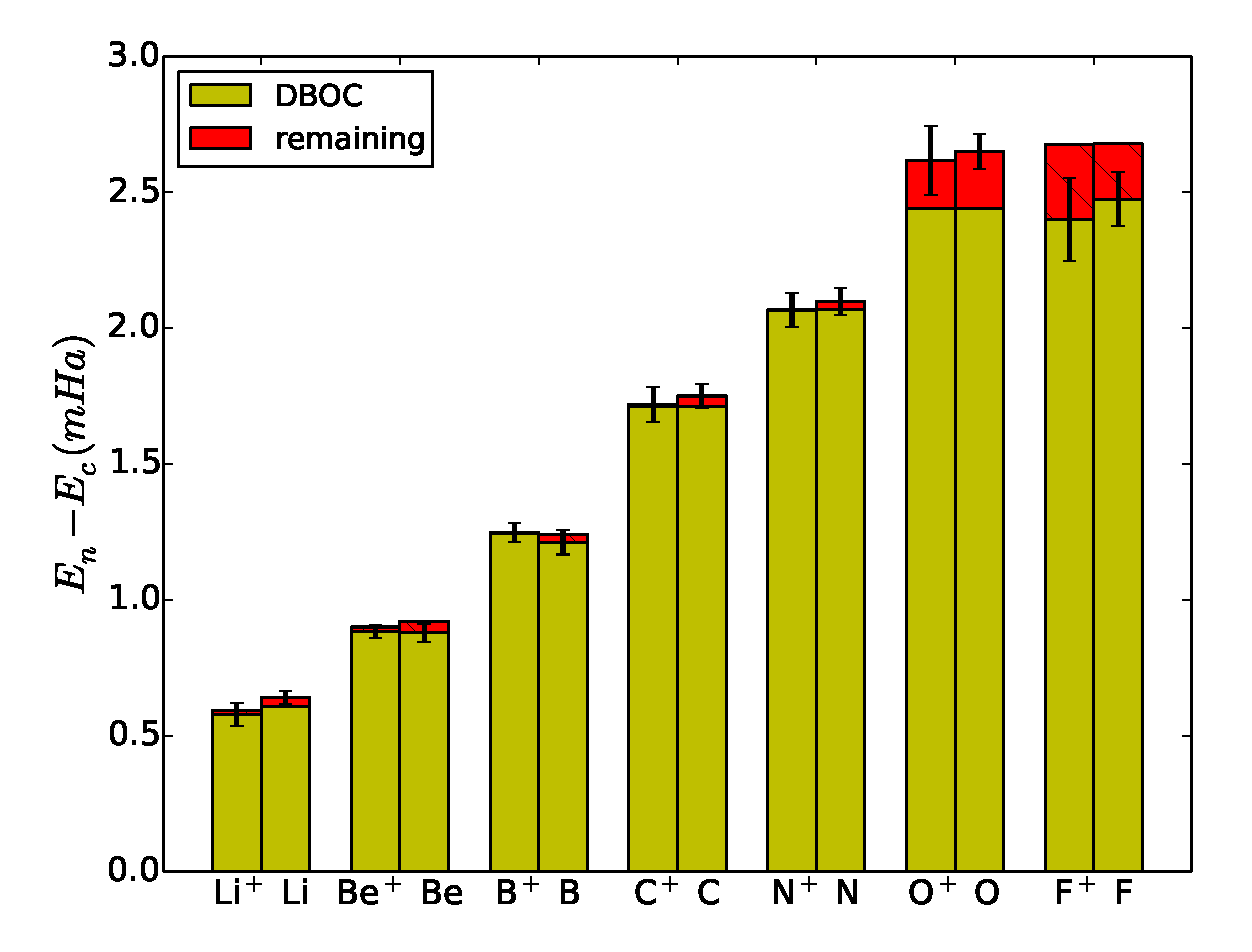
\includegraphics[width=0.8\textwidth]{atom-nad-ad}
\caption{The nonadiabatic contribution to ground-state energies of atoms and ions calculated with FN-DMC. The nonadiabatic contribution is partitioned into the DBOC and the remaining correction. A hatched bar indicates the contribution is negative. The numerical DBOC data is provided in Table \ref{tab:nad-ad-atoms}. \label{fig:atom-nad-ad}} %nonadiabatic contribution shows very little dependence with the ionized state.
\end{figure}

\begin{figure}[h]
\centering
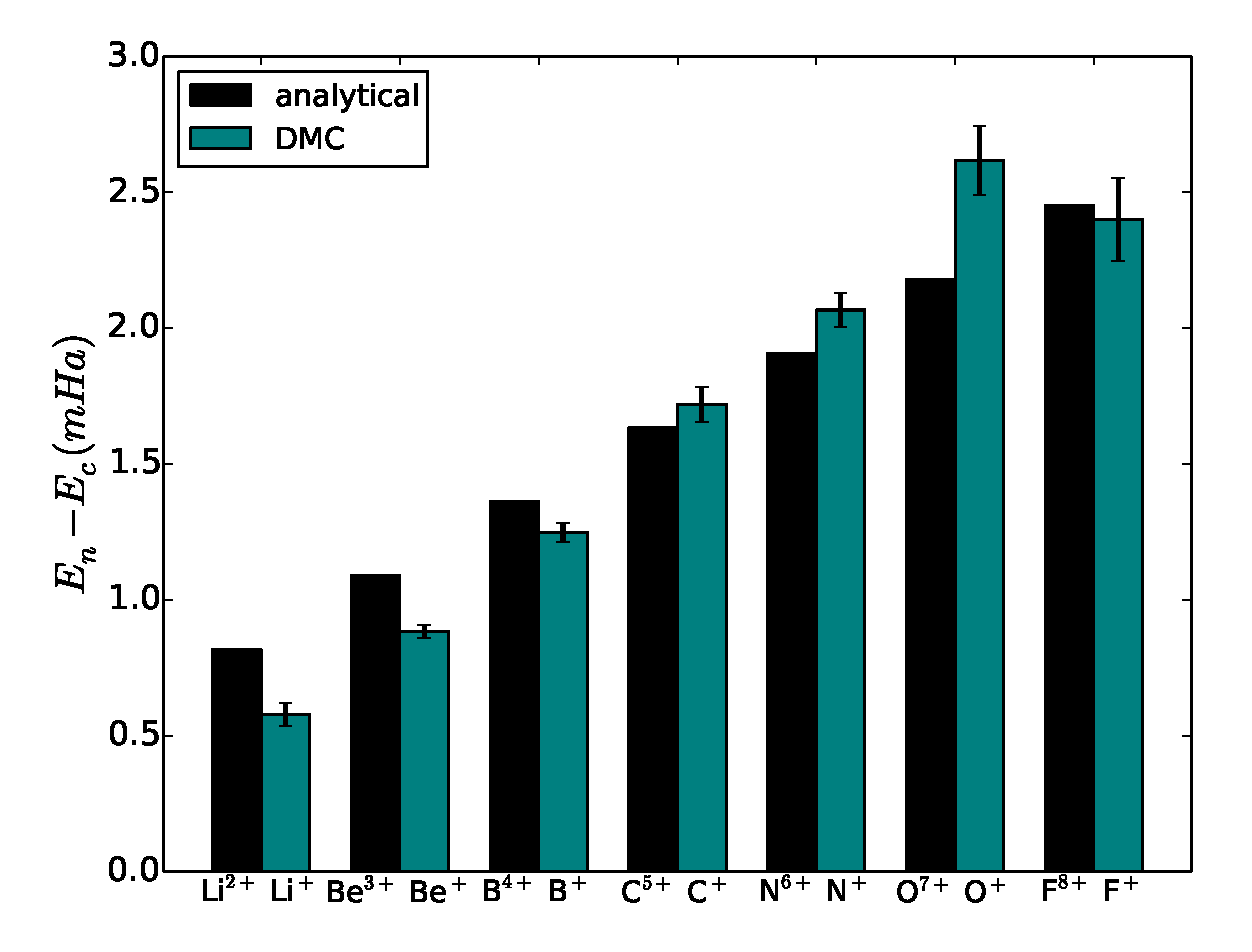
\includegraphics[width=0.8\textwidth]{analytical}
\caption{The nonadiabatic contribution to ground-state energies of ions and their corresponding hydrogen-like atoms calculated with FN-DMC and analytically as shown in Eq. \ref{eq:analytical}. \label{fig:analytical}}
\end{figure}

\begin{table}[h]
\centering
\setlength{\extrarowheight}{1pt}
\caption{Nonadiabatic corrections for the ground-state energies of atoms and ions. $E_n$ and $E_c$ are the FN-DMC calculations of the nonadiabatic and clamped ground-state energies, respectively. The DBOC contribution is provided by Wim Klopper (personal communication). All energies are reported in units of mHa.\label{tab:nad-ad-atoms}}
\begin{tabular}{ccc|ccc}
\hline\hline
System & $E_n-E_c$&  DBOC     & System & $E_n-E_c$&  DBOC \\ \hline
Li$^+$ &   0.58(4) &  0.591970 & Li     &   0.64(2) &  0.608411 \\
Be$^+$ &   0.88(2) &  0.899706 & Be     &   0.88(3) &  0.920848 \\
B$^+$  &   1.25(4) &  1.242988 & B      &   1.21(5) &  1.241669 \\
C$^+$  &   1.72(6) &  1.710382 & C      &   1.75(5) &  1.710900 \\
N$^+$  &   2.07(6) &  2.066914 & N      &   2.10(8) &  2.069149 \\
O$^+$  &   2.6(1) &  2.440320  & O      &   2.6(2)&  2.441821 \\
F$^+$  &   2.4(2) &  2.675128  & F      &   2.5(1)&  2.678181 \\
\hline\hline
\end{tabular}
\end{table}


In Table \ref{tab:nad-ad-atoms} and Figure \ref{fig:atom-nad-ad}, we demonstrate the amount of nonadiabatic contribution to the ground-state energies in atoms and ions calculated as the difference between the nonadiabatic and clamped-ion ground-state energies. The amount of nonadiabatic contribution is always positive for these systems and mostly increases with atomic number. Using previous benchmark values for the DBOC, we can break down the nonadiabatic contribution of our system into a DBOC contribution and everything beyond the DBOC.\footnotemark\footnotetext{The DBOC values for the atoms and ions provided by Prof. Wim Klopper are calculated at the CCSD/d-aug-cc-pwCVQZ level using CFOUR.}\footnotemark\footnotetext{CFOUR, a quantum chemical program package written by J.F. Stanton, J. Gauss, M.E. Harding, P.G. Szalay and others.}~\cite{Harding} The DBOC is relatively insensitive to the level of theory. Figure \ref{fig:atom-nad-ad} indicates that in the atomic systems, the DBOC is the dominant contribution to the nonadiabatic energy, with the remaining amount being close to zero within error bars. The nonadiabatic energy is relatively constant between the neutral and cationic species. This observation suggests that the amount of nonadiabatic contribution is insensitive to the addition or removal of a valence electron. Physically, the valence electrons are farther from the nucleus than the core electrons, thus are likely to be affected to a lesser degree by the delocalization of the nucleus. 

The nonadiabatic contributions in the cations can also be compared with those in their corresponding hydrogen-like atoms for a more in-depth analysis. The nonadiabatic contribution in a hydrogen-like atom can be obtained analytically. The result in Hartree atomic units is
\begin{align}
E_n-E_c=\frac{Z^2}{2}(1-\mu) \label{eq:analytical}
\end{align}
where $\mu=\frac{M}{M+1}$ is the reduced mass of the hydrogen-like atom and $M$ and $Z$ are the mass and atomic number of the nucleus, respectively. The increase in the nonadiabatic contribution with increasing $Z$ for hydrogen-like atoms reflects the stronger Coulombic attraction between the electron and the nucleus, which enhances the effects of the delocalization of the nucleus. An interesting case to consider is the transition from Li$^{2+}$ to Li. As shown in Figure \ref{fig:atom-nad-ad} and Figure \ref{fig:analytical}, the addition of a core electron to Li$^{2+}$ decreases the nonadiabatic contribution, while the addition of a valence electron has no further effect within our error bars. We also calculate the nonadiabatic contribution in Be$^{2+}$ to be $0.78(5)$ mHa, which is $0.29(5)$ mHa lower than the nonadiabatic contribution in Be$^{3+}$ and is closer to that in Be$^{+}$ of 0.88(2) mHa. Because the core electrons interact more strongly with the nucleus than do the valence electrons, the core electrons are affected more by the delocalization of the nucleus. Moreover, the addition of a second core electron decreases the nonadiabatic contribution for Li$^{2+}$ and Be$^{3+}$. %due to correlation with the first core electron.%shielding effects.
We note that the nonadiabatic correction to the atomic ground-state energies of Eq. (\ref{eq:analytical}), which only holds for single electron systems, is roughly linear in Z, while the relativistic recoil correction~\cite{Merkt_H2} scales as $Z^4$. Therefore, the nonadiabatic effect is not seen experimentally,  as it is less significant than this relativistic effect.

\subsection{Hydrides}

\begin{sidewaystable*}[t!]
\setlength{\extrarowheight}{1pt}
\begin{threeparttable}
\caption{Ground-state energies and atomization energies: fixed-node DMC results of this work for all first row hydrides with and without the Born-Oppenheimer approximation. The rows marked with bold \textbf{FN-DMC} are our nonadiabatic results. All atomization energies are estimated for 0K. $D_o$ includes zero-point energy contribution, while $D_e$ does not. Both total energies and dissociation energies are given in units of Hartree. \label{tab:atomization}}
\begin{tabular}
% siunitx setup
{
 l
 S[table-format=1.6]
 S[table-format=4.6]
 S[table-format=4.6]
 S[table-format=4.6]
 S[table-format=4.6]
 S[table-format=4.6]
 S[table-format=4.6]
}

\hline\hline
\multicolumn{1}{c}{Molecule} & 
\multicolumn{1}{c}{LiH$(^1\Sigma^+)$} &
\multicolumn{1}{c}{BeH$(^2\Sigma^+)$} &
\multicolumn{1}{c}{BH$(^1\Sigma^+)$} &
\multicolumn{1}{c}{CH$(^2\Pi)$} &
\multicolumn{1}{c}{OH$(^2\Pi)$} &
\multicolumn{1}{c}{HF$(^1\Sigma^+)$} \\ 
\hline
\multicolumn{1}{c}{} & 
\multicolumn{1}{c}{} &
\multicolumn{1}{c}{} &
\multicolumn{1}{c}{clamped-nuclei} &
\multicolumn{1}{c}{} &
\multicolumn{1}{c}{} &
\multicolumn{1}{c}{} \\
FN-DMC & \text{-}8.070518(7) & \text{-}15.24793(2) & \text{-}25.28867(3) & \text{-}38.4780(1) & \text{-}75.7356(1) & \text{-}100.4552(1) \\
$E_{\text{ref}}$ \tnote{a} & \text{-}8.0705473 & \text{-}15.2483(4) & \text{-}25.2893(2) & \text{-}38.4792(2) & \text{-}75.7382(2) & \text{-}100.4600(3) \\
\multicolumn{1}{c}{} & 
\multicolumn{1}{c}{} &
\multicolumn{1}{c}{} &
\multicolumn{1}{c}{nonadiabatic} &
\multicolumn{1}{c}{} &
\multicolumn{1}{c}{} &
\multicolumn{1}{c}{} \\
\textbf{FN-DMC} & \text{-}8.06624(3) & \text{-}15.24194(5) & \text{-}25.28128(9) & \text{-}38.4672(3) & \text{-}75.7245(5) & \text{-}100.4431(4) \\
ECG \cite{Bubin_LiH_noBO,Bubin_BeH_noBO,Bubin_BH_noBO} & \text{-}8.0664371(15) & \text{-}15.24203(10) & \text{-}25.2803(10) & N/A & N/A & N/A \\
\hline

\multicolumn{1}{c}{} & 
\multicolumn{1}{c}{} &
\multicolumn{1}{c}{} &
\multicolumn{1}{c}{clamped-nuclei} &
\multicolumn{1}{c}{} &
\multicolumn{1}{c}{} &
\multicolumn{1}{c}{} \\
$D_e$ (FN-DMC) & 0.09246(1) & 0.08062(2) & 0.13493(3) & 0.1335(1) & 0.1699(2) & 0.2234(1) \\
$D_e$ Feller \tnote{b} & 0.09262(5) & 0.0809(4) & 0.1354(2) & 0.1342(2) & 0.1709(2) & 0.2258(3) \\
\multicolumn{1}{c}{} & 
\multicolumn{1}{c}{} &
\multicolumn{1}{c}{} &
\multicolumn{1}{c}{nonadiabatic} &
\multicolumn{1}{c}{} &
\multicolumn{1}{c}{} &
\multicolumn{1}{c}{} \\
$D_o$ (\textbf{FN-DMC}) & 0.08910(4)  & 0.07578(6)  & 0.1290(1) & 0.1248(3) & 0.1617(5) & 0.2141(4) \\
$D_o$ Feller \tnote{c} & 0.08940(5) & 0.0761(4) & 0.1299(2) & 0.1276(2) & 0.1622(2) & 0.2166(3)\\
$D_o$ Exp. \cite{CCCBDB,HH} & 0.08874(38) & 0.07475(4) & 0.1281(37)\tnote{d} & 0.1275(5) & 0.1622(1) & 0.2158(3) \\
\hline\hline
\end{tabular}
\begin{tablenotes}
\item[a] For LiH, ECG provides the best reference energy.~\cite{Adamowicz_LiH} For the rest of the systems, we combined the best clamped-ion atomic references in Table \ref{tab:ionization} and thermochemistry estimates of $D_e$ in this table to produce the reference ground-state energies.
\item[b] Estimates for $D_e$ are calculated by subtracting the scalar relativistic, spin-orbit coupling and zero-point energy corrections from the reference $D_o$ in Table VI of Ref.~\cite{Feller_Corrections}.
\item[c] Here only the scalar relativistic and spin-orbit coupling corrections are subtracted.
\item[d] The atomization energy for BeH in Ref.~\cite{CCCBDB} disagrees with previous high-level theoretical benchmarks,~\cite{Feller_Corrections,Bubin_BeH_noBO} thus we use Ref.~\cite{HH} instead. For several of the systems, multiple experimental values are available in the literature.  We report experimental values that were aggregated in one single reference,~\cite{CCCBDB} except for BeH.~\cite{HH}
\end{tablenotes}
\end{threeparttable}
\end{sidewaystable*}
In Table \ref{tab:atomization}, we present our results on a series of molecular systems (hydrides). Finding accurate reference data for these systems to 0.1 mHa is not straightforward. We will use highly converged ECG data when available. Two ECG calculations have been performed in the clamped-nuclei limit for LiH~\cite{Cencek_LiH,Adamowicz_LiH} and we agree within 0.03 mHa with the more recent reference. For the rest of the systems, we combined the best clamped-ion atomic references in Table \ref{tab:ionization} and thermochemistry~\cite{Feller_Corrections} estimates of atomization energy $D_e$ in Table \ref{tab:atomization} to produce the reference ground-state energies. For BeH and BH, we are within 1 mHa of the reference values, and our energies are lower than the best available quantum chemistry results of -15.247846 Ha~\cite{Koput_BeH} and -25.287650 Ha~\cite{Miliordos_BH} for BeH and BH, respectively. 
%For the rest of the systems it is possible we have the lowest variational estimates. %, but a comparison with reference suggests that we have fixed-node error in the range of a few mHa.

\begin{figure}[h]
\centering
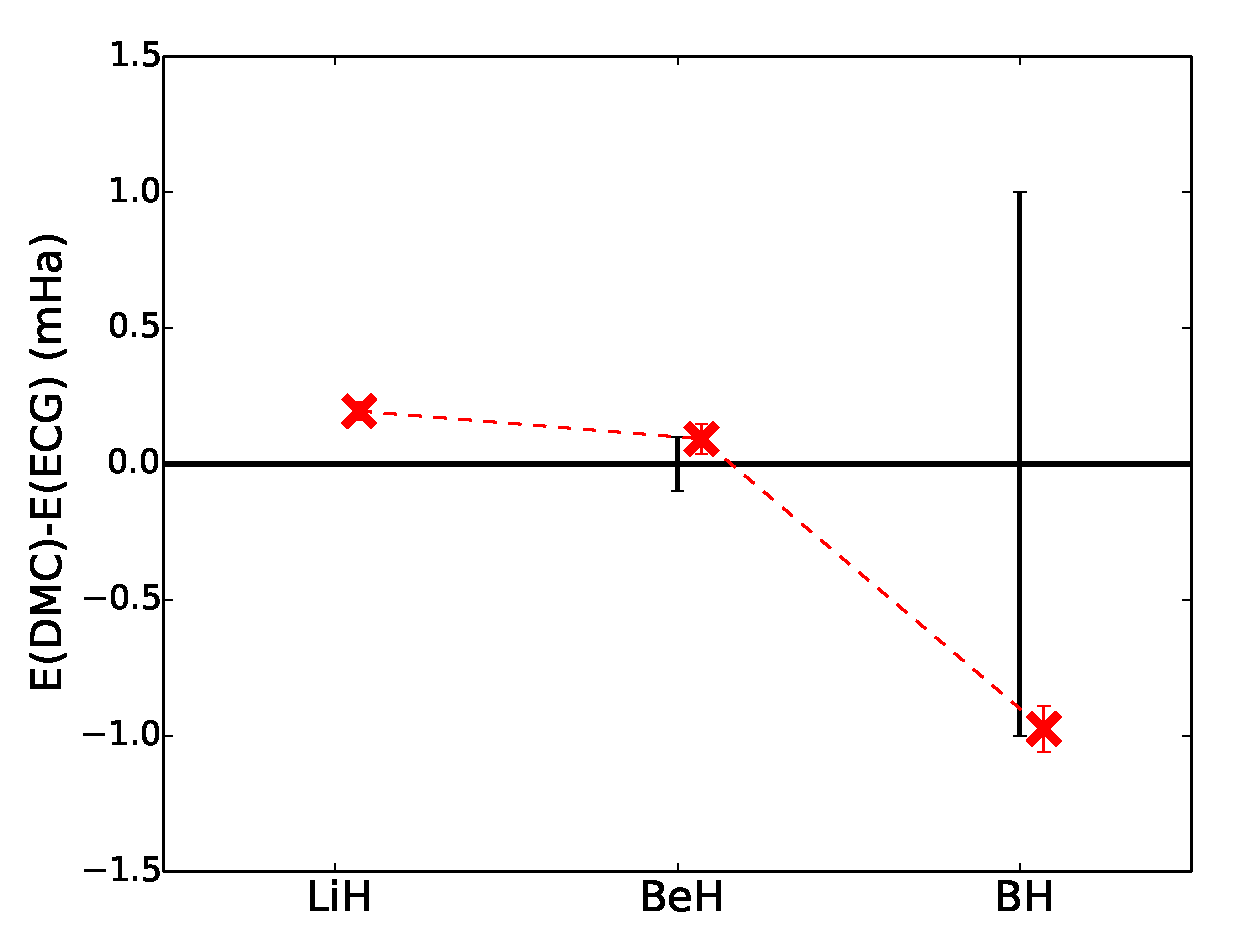
\includegraphics[width=0.8\textwidth]{dia-ECG}
\caption{The nonadiabatic FN-DMC ground-state energies of LiH, BeH and BH relative to ECG references. The error bars for the nonadiabatic ECG references are shown as thick dark lines, and the error bars for the FN-DMC calculations are comparable to the size of the symbols. \label{fig:dia-ECG}}
\end{figure}

Nonadiabatic ECG calculations only exist for the three smallest hydrides. Our results for LiH and BeH agree with the ECG references to within 0.2 mHa, as shown in Figure \ref{fig:dia-ECG}. The ECG reference for LiH is converged to the true ground-state energy beyond 0.1 mHa; thus, it is likely that our wave function has a fixed-node error of 0.2 mHa. For BeH, our result is within 0.1 mHa of the ECG reference and agrees within error bars. With BH being one of the largest ECG simulations performed, the DMC result is actually lower in energy, in this case by 1 mHa. The ECG error bar on BH is large, and it is not evident how close our result is to the true ground state, although extrapolating the ECG result with basis set size suggests we are within 1 mHa.~\cite{Bubin_BeH_noBO} For these nonadiabatic systems, we have the lowest variational result for BH, and the only simulated results of for CH, OH, and HF, to the best of our knowledge.

The atomization energies of the diatomic systems are reported in Table \ref{tab:atomization}. High-quality thermochemistry benchmarks are used for comparison.~\cite{Feller_Corrections} We take the reference energies from the last column of Table VI of Ref.~\cite{Feller_Corrections} and subtract the corrections in the $\Delta E_{SR}$ (scalar relativistic) and SO (spin-orbit coupling) columns for the comparison with our non-relativistic energies. For the comparison with our clamped-nuclei results, we further subtract the DBOC and ZPE (zero-point energy) corrections.
%Corrections from spin-orbit coupling and relativistic effects are not used, as they are not included in our Hamiltonian.
The atomization energies estimated in the clamped-nuclei limit agree within 1 mHa of the references for all but the largest molecule, HF. Within quantum Monte Carlo, it is generally more difficult to obtain an accurate nodal surface for a molecule than for an atom. As a result, our estimates for the clamped-nuclei atomization energies are lower than the references in all cases. A similar trend can be observed when comparing our nonadiabatic results with the references. For each molecule, the deviation from the reference is similar in the clamped-nuclei and nonadiabatic cases except for CH.

\begin{figure}[h]
\centering
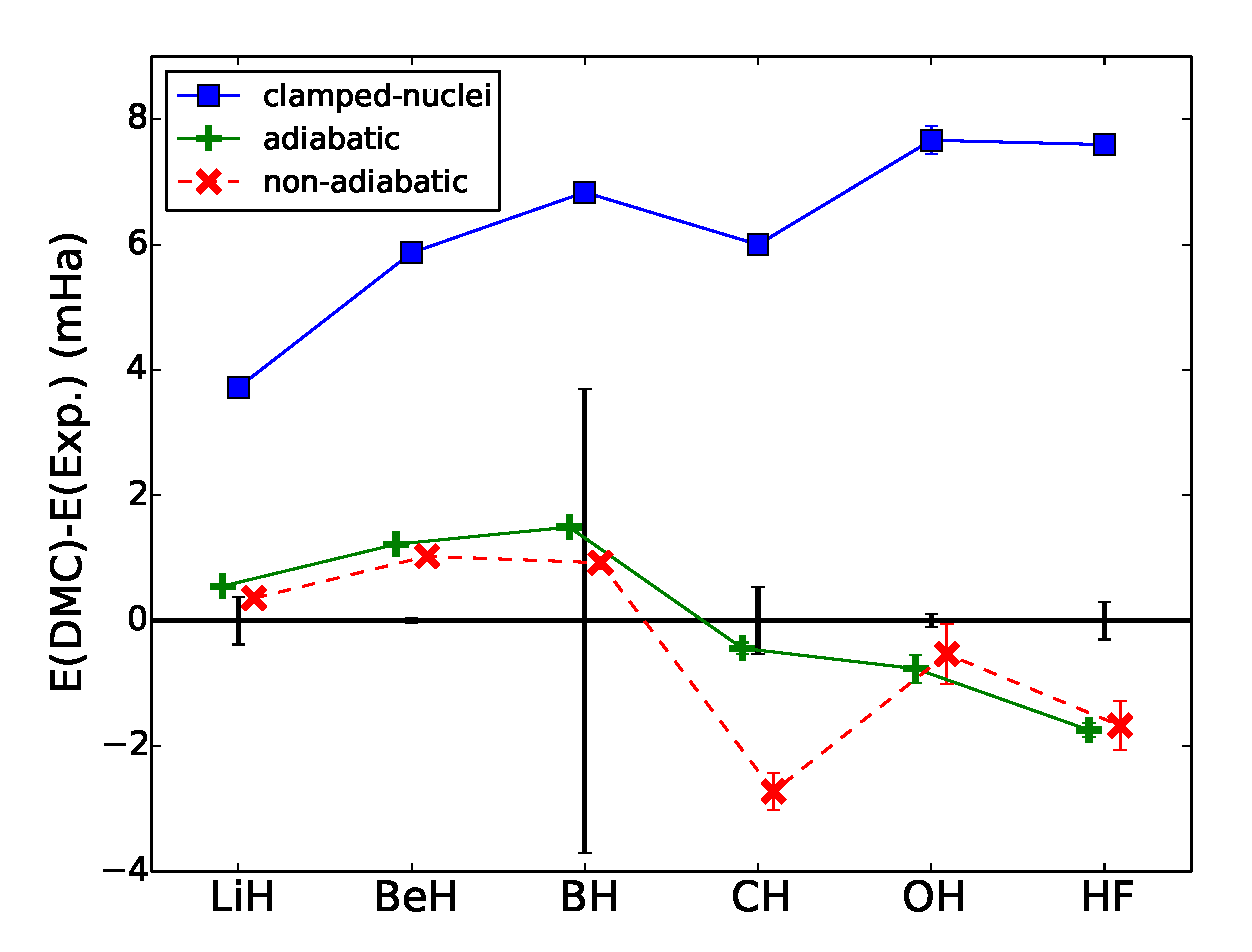
\includegraphics[width=0.8\textwidth]{atomization}
\caption{Atomization energies of first row hydrides obtained with FN-DMC relative to experimental data. The adiabatic results are estimated by adding zero-point energies from Ref.~\cite{Feller_Corrections} to the clamped-nuclei results. \label{fig:atomization}}
\end{figure}

In Figure \ref{fig:atomization}, we compare both our clamped-nuclei and our nonadiabatic results to experimental data. We also provide adiabatic estimates by adding the zero-point energies calculated with coupled-cluster techniques in Ref.~\cite{Feller_Corrections} to our clamped-nuclei results. To calculate experimental atomization energies starting from the clamped-nuclei results, energetic corrections due to zero-point motion of the nuclei, nonadiabatic effects, spin-orbit coupling and relativistic effects should be included. For these highly adiabatic systems, the inclusion of zero-point motion alone is sufficient to bring our clamped-nuclei results to within 2 mHa of the experimental results. Except for the case of CH, the nonadiabatic results agree closely with their adiabatic counterparts and are closer to the experimental values, although for BH the experimental error bar is too large to provide a high-accuracy comparison. For CH, the experimental result suggests that our electron-ion wave function for this molecule has an unusually large fixed-node error.

\begin{figure}[h]
\centering
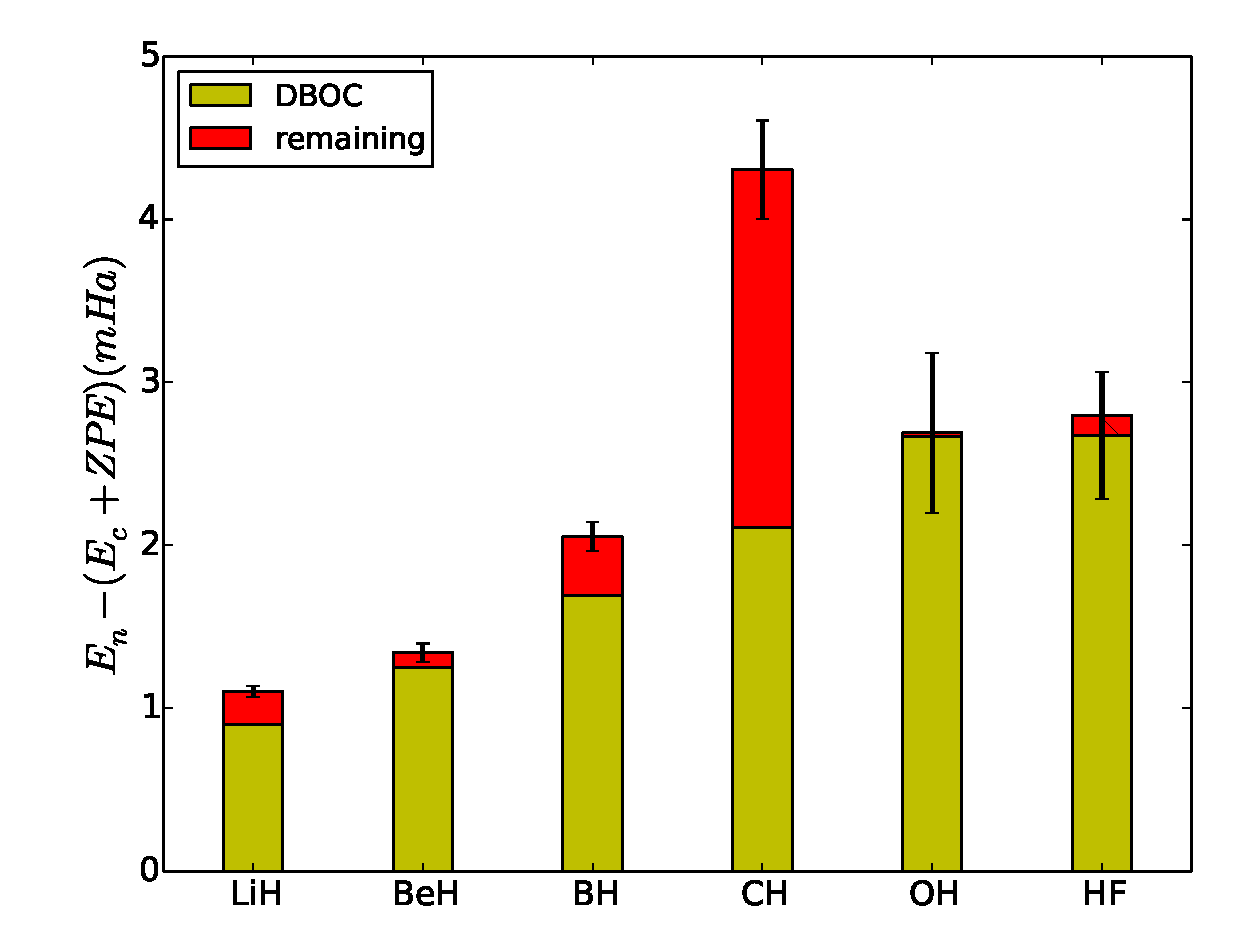
\includegraphics[width=0.8\textwidth]{dia-nad-ad}
\caption{The nonadiabatic contribution to the ground-state energies in hydrides calculated with FN-DMC. The adiabatic reference energies are calculated by adding zero-point energy contributions from Ref.~\cite{Feller_Corrections} to our clamped-nuclei results. The nonadiabatic contribution is partitioned into the DBOC and the remaining correction. A hatched bar indicates the contribution is negative. \label{fig:dia-nad-ad}}
\end{figure}

To estimate the nonadiabatic contribution to the ground-state energies for these hydrides, we calculate the difference between our nonadiabatic and adiabatic results, as shown in Figure \ref{fig:dia-nad-ad}. Similar to the atomic case, we break down the nonadiabatic energy of our system into a DBOC contribution and everything beyond the DBOC.\footnotemark\footnotetext{The DBOC references provided by Prof. David Feller are calculated at the CCSD(T)/aug-cc-pVTZ level using CFOUR}~\cite{Harding} The ZPE and DBOC contributions to this difference are listed in Table \ref{tab:nad-ad-diatomics}. We also calculate the nonadiabatic correction to the dissociation energies of the hydrides.
%The total amount of nonadiabatic contribution appears to peak for CH, although this larger contribution may reflect the larger fixed-node error for this system. 
For BeH, OH, and HF, the nonadiabatic contribution is almost entirely accounted for by the DBOC with the remaining correction being zero within error bars. For LiH, BH, and CH, the remaining amount of nonadiabatic contribution seems to be nonzero, and appears quite significant in CH. However, if the electron-ion wave function is significantly lower in quality than the electronic wave function for a given system, then the amount of nonadiabatic contribution will be overestimated. We also use the zero-point energies from Feller et. al.~\cite{Feller_Corrections} as corrections, which may introduce some additional uncertainty.  Regardless, our current predictions suggest that nonadiabatic effects in BH and CH are larger than in the other systems we considered.

For the LiH molecule, we also calculated the electron affinity for comparison to ECG results. We calculated the ground-state energy of LiH$^-$ to be $-8.08222(2)$~Ha for the case of clamped-nuclei. With nonadiabatic effects included, our result is  $-8.07811(3)$~Ha. Our nonadiabatic result is in good agreement with a previous ECG study,~\cite{Bubin_LiH-_noBO} which reported a value of $-8.07856887$~Ha. We report an electron affinity of $0.01187(4)$~Ha, which can be compared to the ECG prediction of $0.012132(2)$~Ha and agrees with the experimental value of $0.0126(4)$ Ha.\footnotemark\footnotetext{We note that LiH ground state energies which we compare against are mislabeled in Ref.~\cite{Bubin_LiH-_noBO}, with $\text{LiH}^-$ and LiD being switched.}

\begin{table}[h]
\centering
\setlength{\extrarowheight}{1pt}
\caption{Nonadiabatic corrections for the ground-state energies of diatomic molecules. $E_n$ and $E_c$ are the FN-DMC calculations of the nonadiabatic and clamped ground-state energies, respectively. The ZPE and DBOC contributions are provided by David Feller (personal communications).The nonadiabatic correction for the dissociation energy estimated with FM-DMC are included in the $\Delta D_o$ column. All energies are reported in units of mHa.\label{tab:nad-ad-diatomics}}
\begin{tabular}{ccccc}
\hline\hline
System & $E_n-E_c$ &   ZPE &      DBOC & $\Delta D_o$\\ \hline
LiH  &   4.28(3) &  3.17 &  0.902410 & -0.19(4) \\
BeH  &   5.99(6) &  4.65 &  1.251000 & -0.19(6) \\
BH   &   7.39(9) &  5.34 &  1.692559 & -0.6(1) \\
CH   &  10.8(3) &  6.44 &  2.109487  & -2.3(3)  \\
OH   &  11.1(5) &  8.43 &  2.670397  &  0.2(5)  \\
HF   &  12.0(4) &  9.34 &  2.799624  &  0.1(4)  \\
\hline\hline
\end{tabular}
\end{table}

% beyond dragged node 
\subsection{Dragged Node Approximation}
In our current approach, the fixed-node approximation generally causes an overestimate the nonadiabatic effects. This is a result of the increased complexity of optimizing wave functions for the full electron-ion system. When the clamped-ion energies are more accurate than the electron-ion energies, we overestimate the nonadiabatic energy. It should be noted that in some cases the energies for the full electron-ion simulations can be more accurate than for the corresponding clamped-ion simulations, as suggested by the comparisons of Be, Be+, B, B+, and C+ in Fig.~\ref{fig:ionization}.
However, this is less likely for molecular systems in which the ions can move relative to each other.
All our simulations up to this point have used a particular type of approximation to the nodal structure called the dragged-node approximation.
This approximation can be used for wave functions in the form of Eq.~\ref{eq:psi_gms} in which we start by generating a wave function defined at the equilibrium geometry.
When the ions change position the wave function changes based on the basis set dependence of the ion coordinates.
The change in the wave function causes a corresponding change in the nodes.
The dragged-node approximation is completely variational when used in FN-DMC.
For systems that do not show strong nonadiabatic behavior the dragged-node approximation should yield excellent results.
It was surprising that the energy contribution from nonadiabatic effects of the CH molecule was larger than other hydrides, indicating that we might need to use better wave function forms to accurately simulate CH.

\subsection{Improving Wave Functions}
We can improve the electron-ion wave function by updating the electronic part using quantum chemistry rather than relying on the dragged-node approximation
\begin{align}
\Psi_{CISD}(\bs{r},\bs{R}) &= \sum_i c_i(\bs{R}) \phi_i(\bs{r},\bs{R}_o), \label{eq:nonbo-best-psi}
\end{align}
where the determinant expansion coefficients $c_i(\bs{R})$ now depend on the positions of the ions as opposed to being fixed to their equilibrium values as in Eq.~\ref{eq:psi_gms}.

The wave function in Eq.~\ref{eq:nonbo-best-psi} is more general than Eq.~\ref{eq:psi_gms}
but is more difficult to generate. In practice, it is not feasible to regenerate both the orbitals and expansion coefficients for each new configuration of the ions.
However, for diatomic molecules we can precompute and optimize wave functions at different distances and then use the precomputed wave functions to interpolate wave function amplitudes at other ion positions.
There are several different ways this can be done.
The first approach we considered is to use a grid of bond lengths and calculate a fully optimized electronic wave function at each grid point.
Then one would calculate the electronic wave function at each grid point and use an interpolation scheme to determine the electron-ion wave function.
Although technically feasible, we found it difficult to maintain a smooth wave function within this approach.
A second approach, for which we present results here, parameterizes the
determinant coefficients as a function of the ion positions.
For a diatomic system, this corresponds to generating a 1D function for each determinant coefficient.
This is an improvement over the dragged-node approximation, because the coefficients of the determinants are allowed to change with ion distance and can capture complicated ion dependence of the node.
%In future work, it may also be possible to extend this type of wave function to at least three particles, which would require fitting functions for the determinant coefficients in higher dimensions.

We tested the improved wave function Eq.~\ref{eq:nonbo-best-psi} for the CH molecule by implementing the following additional steps. At the equilibrium C-H separation $R_o$=2.1165 a.u., we optimize the electronic wave function, which includes all determinant coefficients and a Jastrow. At two C-H separations near equilibrium $R_{left}$=2.0 a.u., $R_{right}$=2.25 a.u., we reoptimize only the determinant coefficients of the electronic wave function, keeping all other parameters fixed. For each determinant coefficient, we approximate its dependence on the distance between the ion separations $R$ using a linear interpolation
\begin{align}
c_i^*(R) = c_i(R_{\text{left}}) + 
\dfrac{c_i(R_{\text{right}}) - c_i(R_{\text{left}})}{R_{\text{right}}-R_{\text{left}}}\times(R-R_{\text{left}}). \label{eq:interpolation}
\end{align}

\subsection{Results and Discussion}
We present here a diagnostic test to determine when this type of improvement might be important.
The potential energy surface as a function of the C-H distance is plotted for several different nodal surfaces in Figure~\ref{fig:ch-cold}.
In particular, we calculate clamped-ion energies that correspond to the dragged-node approximation as well as energies from a linear interpolated wave function as given by Eq.~\ref{eq:interpolation}.
The reference result is obtained by re-optimizing the Jastrow factor and the determinant coefficients at every C-H separation.
The region for the most probable ion distances is indicated by the vertical dashed lines.
Over the region of important ion separations, the potential energy surface from the interpolated wave function is improved over the dragged-node potential energy surface when compared to the fully optimized potential energy surface.
Further away from the region of interest, both the dragged-node and the interpolated wave functions deviate significantly from reference data.
However, this region is seldom sampled during our FN-DMC simulations and is not expected to introduce a large bias into our results.

\begin{figure}[h]
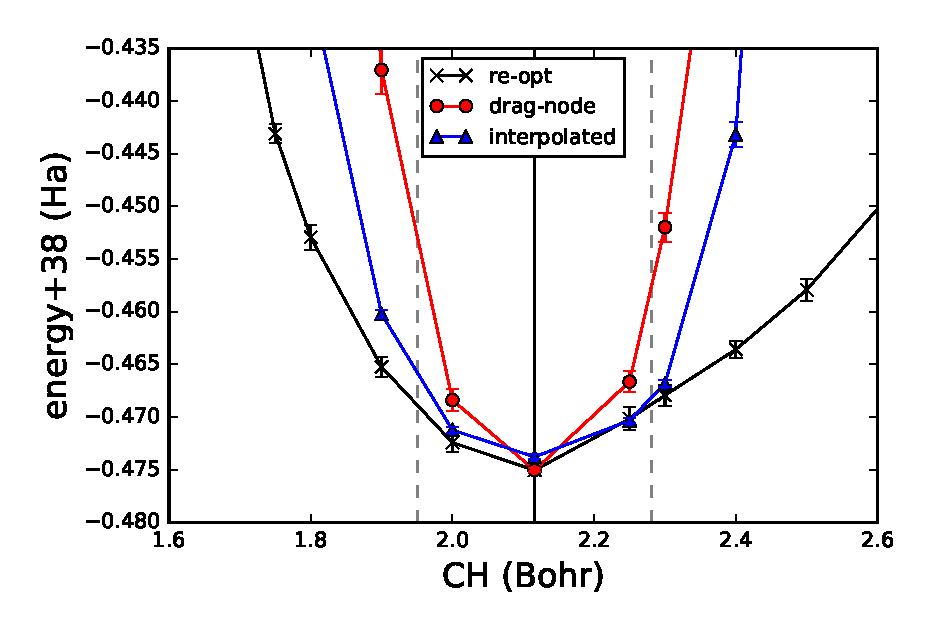
\includegraphics[width=0.8\textwidth]{ch-cold}
\caption{Clamped-ion VMC total energy as a function of C-H separation using a hierarchy of wave functions. The dashed lines mark the FWHM of the distribution of C-H separation.  Within the region marked by the dashed lines it can be seen that the interpolated wave function results are a closer match to the reference 're-opt' energies than the dragged-node energies. \label{fig:ch-cold}}
\end{figure}

%In our previous study, wave functions of the form in Eq. (2) were used to
%simulate several different molecular systems (6).
To determine the nonadiabatic contribution for each system,
we partition the energy into different components,
which includes the clamped-ion energies, the zero point energy (ZPE) and the
diagonal Born-Oppenheimer correction (DBOC). Everything that remained we
consider to be the nonadiabatic energy. Using standard quantum chemistry tools
all of the above terms can be calculated or approximated to high accuracy with
the exception of the nonadiabatic energy. As a result the nonadiabatic energy is
a quantity that has not been theoretically calculated for many systems. We see from Fig.~\ref{fig:dia-nad-ad} that the nonadiabatic energy was less than 0.1 mHa for most of the
systems considered. There are two exceptions, where the nonadiabatic energy
was larger, for the cases of BH and CH molecules.
Our new results for CH with the improved wave functions can be seen in Table~\ref{tab:nad-ch-energy}. Due to the variational property of FN-DMC, it is evident that these energies
are improved over the previous best results for the CH molecule, which is not
unexpected given the differences between the interpolated wave function and the
dragged-node wave function as seen in Figure~\ref{fig:ch-cold}. Our previous results showed a
nonadiabatic energy of 1.9 mHa, whereas our new results show a nonadiabatic energy of
0.9 mHa, which can be seen for the largest determinant expansion in Table~\ref{tab:nad-ch-energy}. This
is consistent with our previous results, mainly that the CH molecule is somewhat
nonadiabatic, even though our new estimate of the nonadiabatic energy is smaller.
For a system with a moderate amount of nonadiabatic energy, more effort is needed
in generating accurate wave functions. Improving the wave functions beyond the
dragged-node approximation will lower the estimate of the nonadiabatic energy,
but it is likely to remain somewhat large if the improvements of the wave function
correspond to degrees of freedom beyond the Born-Oppenehimer approximation.
This is what we see for CH, as the nonadiabatic energy is still relatively large in
comparison to other systems. We note that this is still not a definitive estimate of
the nonadiabatic energy, but it is likely the best estimate ever calculated for this
system.

\begin{table}[h]
\centering
\caption{DMC energy and variance with static ions, dynamic ions with dragged-node (``drag'') and dynamic ions with determinant coefficient interpolation (``interp.'').\label{tab:nad-ch-energy}}
\begin{tabular}{llll}
\hline\hline
$N_{\text{det}}$ & Energy (Ha) & Variance (Ha$^2$) & method \\
\hline
35   & -38.4709(1) &  0.3130(5) &    static \\
35   & -38.4622(2) &  0.3169(3) &   drag \\
35   & -38.4621(2) &  0.3173(3) &  interp. \\
723  & -38.4770(1)&  0.2489(3) &    static \\
723  & -38.4667(1) &  0.334(2)~  &   drag \\
723  & -38.4679(1) &  0.2713(7) &  interp. \\
4739 & -38.4781(1) &  0.2300(4) &    static \\
4739 & -38.4676(1) &  0.334(5)~  &   drag \\
4739 & -38.4687(2) &  0.267(7)~  &  interp. \\
\hline\hline
\end{tabular}
\end{table}

We also noticed interesting behavior that results from improving the quality
of the electron nodes. We performed clamped-ion (static) and fully nonadiabatic
(dynamic) calculations using different truncations levels for the determinant
expansion. The FN-DMC energy and variance for the various calculations are
shown in Table~\ref{tab:nad-ch-energy}. As we include more determinants in our wave function,
both the energy and variance of the static calculation decrease. However, the
same does not happen for the variance of the dragged-node approximation, in
which we see the surprising result that the variance increases. This suggests
that the clamped-ion wave functions are being improved to a larger extent than
the dragged-node wave functions with increasing determinant number. It is also
interesting to note that for the wave functions with the smallest determinant
expansion ($N_{det}$ = 35), the variance is almost the same between the clamped-ion
and dragged-node wave functions.
The energy and variance with determinant coefficient interpolation is
generally improved from our previous wave function with the dragged-node
approximation. A comparison between the dynamic runs with and without
interpolation also shows that coefficient interpolation becomes more important
for larger determinant expansions. In particular, the variance improves with
increasing determinant number, showing similar behavior to that of the static
wave function.

\begin{figure}[h]
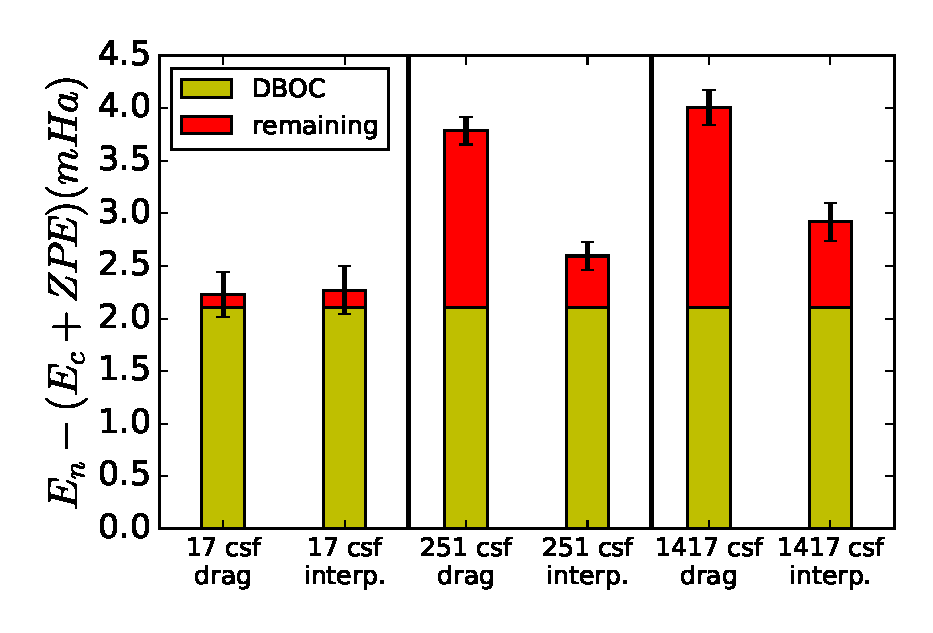
\includegraphics[width=0.8\textwidth]{ch-only}
\caption{Nonadiabatic energy of CH with and without determinant coefficient interpolation.  The wave function ``interp'' denotes that the determinant coefficients depend on C-H separation through linear interpolation. For the largest two determinant expansions a more significant contribution from nonadiabatic effects is observed than the smallest determinant expansion. \label{fig:ch-interp} }
\end{figure}

In Figure~\ref{fig:ch-interp}, we show the various contributions to the difference between
the static and dynamic ground-state energies. Due to the difference in energy
scales for the quantities of interest, we only plot the diagonal Born-Oppenheimer
energy and the nonadiabatic energy. To calculate the nonadiabatic energy we
take the estimated zero-point energy for CH to be 6.438 mHa~\cite{Feller_Corrections}. The diagonal
Born-Oppenheimer correction is estimated to be 2.11 mHa. Our best result is
given by the 4739 determinant interpolated wave function in Figure~\ref{fig:nonbo-ch-star}. There is an apparent increase in the nonadiabatic energy of the CH molecule that results
from using the dragged-node approximation. The improvement seen by using the
interpolated wave function instead of the dragged-node approximation is 1 mHa
for the CH molecule; a relatively large change in the energy.
That the dragged-node approximation produced such a large error
for the CH molecule suggests at the very least that the nodal structure of its wave
function has more complex dependence on the ion configuration than the rest of
the molecules under consideration.

\begin{figure}[h]
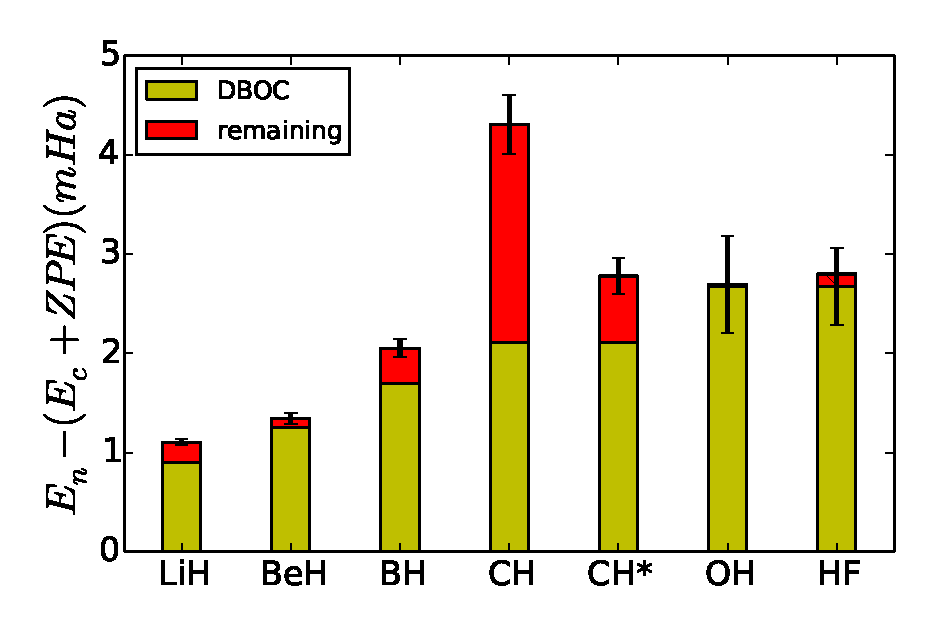
\includegraphics[width=0.8\textwidth]{4738}
\caption{Nonadiabatic energy of diatomic molecules. The best (4739
determinant) result for CH with determinant coefficient interpolation is shown
with *. Note that for all the molcules except for BH and CH the nonadiabatic
energies are roughly 0.1 mHa or smaller.}
\label{fig:nonbo-ch-star}
\end{figure}

Figure~\ref{fig:ch-interp} also reveals that the nonadiabatic energy is only observed with the
large determinant expansions. There are several possible explanations for this. It
is possible we are optimizing the static wave function significantly better than the
electron-ion wave function. There is some indication of this from the variance
of the dragged-node approximation, but this is less evident for the interpolated
wave function. Another possible explanation is that only when the wave function
is highly optimized do significant changes arise in the wave function amplitudes
with regard to ion positions. A related effect is that large fluctuations of the ion
distance can be suppressed if the wave function and the related nodal surface is
not well optimized at large ion distances. Such effects can be mitigated
with the interpolated wave function approach, and are likely to be suppressed with
increasing the number of determinants for the electronic part of the wave function,
even for the dragged-node wave function. In Fig.~\ref{fig:nonbo-ch-star}, we compare our improved results
for CH with the nonadiabatic contributions from previous work. It is evident
that the CH nonadiabatic energy is still larger than all the other molecular
systems.

\section{Conclusion}
We calculated the ground-state energies of first-row atoms and their corresponding ions and hydrides with and without the Born-Oppenheimer approximation. In addition, we examined the amount of nonadiabatic contribution to the ground-state energies of all systems studied and determined the amount to be up to a few mHa. In the case of CH, the nonadiabatic effects beyond the DBOC appeared to be unusually large, although we found that a large part of this discrepancy was due to the fixed-node error.
To this end, we improved the electron-ion wave functions for diatomic systems by interpolating determinant coefficients as a function of ion separation.
Even with the improved wave function, there is still a slightly larger contribution from nonadiabatic effects in CH.

We found the ionization energies of the atoms to be independent of the Born-Oppenheimer approximation, consistent with a previous high-level quantum chemistry study.~\cite{Klopper_IP} In contrast, the atomization energies of the hydrides showed effects of nonadiabaticity, although they were generally much less than 1 mHa. This work obtained the first nonadiabatic QMC benchmark data for non-relativistic ground-state energies and obtained the lowest variational result for BH and the only results for CH, OH and HF, to the best of our knowledge.

%In comparing to accurate benchmark results obtained with other methods, we have demonstrated the validity of our wave function ansatz, namely it does produce a high-quality electron-ion wave function. This technique also has the potential to solve interesting larger-scale problems due to its ease of implementation, as well as the polynomial scaling in computational time with respect to the number of electrons.

%\bibliography{nonbo-ref}
%\printbibliography[heading=general]
\section{Introduction}
There have been several recent discoveries~\cite{Tubman_ECG,cederbaum1,gross2014,boent,Martinez_Review} suggesting that quantum wave functions, which include both electronic and ionic degrees of freedom, have many interesting properties that have yet to be explored.  This includes the development of equations that exactly factorize a wave function into electronic and ionic components,~\cite{cederbaum1,cederbaum12} the disappearance of conical intersections in wave functions of model systems,~\cite{gross2014} and the use of quantum entanglement to study electronic and ionic density matrices.~\cite{boent} Extending such studies to realistic systems is of broad interest and will considerably expand our understanding of electron-ion systems. However, treatment of \textit{ab initio} electron-ion systems is challenging, and applications have thus been limited. The most accurate simulations of electron-ion wave functions are generally done with very specialized wave functions, which are limited to rather small systems.~\cite{mitroy2013} Methods are also being developed to treat larger systems with different regimes of validity.~\cite{Sharon_NEO-HF,Sharon_XCNEO-HF1,Sharon_XCNEO-HF2,Sharon_XCNEO-HF,Kurt_XCNEO-HF,Kurt_XCNEO-HF1,Sharon_NEO-DFT,Sharon_NEO-DFT2,Sharon_NEO-DFT3,Gross_NEO-DFT,Gross_NEO-DFT1,Ilkka_Path,Ilkka_Path1,Ilkka_Path2}

As a framework to address these problems in general realistic systems, we recently demonstrated that quantum Monte Carlo (QMC) can be combined with quantum chemistry techniques to generate electron-ion wave functions.~\cite{Tubman_ECG} We treated realistic molecular systems and demonstrated that our method can be scaled to larger systems than previously considered while maintaining a highly accurate wave function. In the following, we extend our previous work by considering the simulation of a larger set of atoms and molecules. We calculate ionization energies and atomization energies that can be directly compared with previous results for benchmarking purposes.

\section{Method}
\subsection{Fixed-Node Diffusion Monte Carlo (FN-DMC)}
Diffusion Monte Carlo~\cite{Anderson_DMC,lester1,Stuart_Review,Needs_Review,Needs_Old_Review,QMC_Review} is a projector method that evolves a trial wave function in imaginary time and projects out the ground-state wave function. For practical simulations of fermions, the fixed-node approximation is introduced, which depends only on the set of electronic positions where a trial wave function is equal to zero.  This approximation is different than approximations typically used in quantum chemistry calculations. In this work, we demonstrate that we can generate high-quality nodal surfaces for a range of systems that include full electron-ion wave functions. 

If the trial wave function has the same nodal surface as the exact ground-state wave function, FN-DMC will obtain the exact ground-state energy.  Approximate nodal surfaces can be generated through optimization of the full wave function. Such approximate nodal surfaces have been tested and validated on a wide range of systems, and consistently provide an excellent approximation of the exact ground-state energy, comparable to the state of the art in \textit{ab initio} simulations.~\cite{grossman1} In addition, the energies generated with FN-DMC are variational with respect to the ground-state energy.

In all but a handful of previous QMC simulations,~\cite{Ceperley_1987,Natoli_1993,Natoli_1995,Chen_1995,Coldwell_H2_2008,Gabriele_H2_2004,Sandro_finiteT-noBO_2012} calculations are performed with nuclei ``clamped" to their equilibrium positions. However, such an assumption is not fundamentally required by FN-DMC. %In our previous work we find that the most important effects for optimizing are the nodes due to electron-electron correlation~\cite{Tubman_ECG}, and in this regard we use more sophisticated terms in the electronic part of the wave function than in the ionic part.

\subsection{Electronic Wave Function and Optimization}

There are several different approaches for generating electronic wave functions for a FN-DMC calculation.~\cite{Umrigar_Alleviation,Toulouse_Bench,Brown_Bench,Seth_Bench} Recent advances~\cite{Nightingale_Linear,Umrigar_Linear,Brown_Bench} have made it possible to simultaneously optimize thousands of wave function parameters using variational Monte Carlo with clamped nuclei. We use an initial guess for the wave function that is generated from complete active space self-consistent-field (CASSCF)~\cite{Chaban_MCSCF,Szabo} calculations using the quantum chemistry package GAMESS-US.~\cite{GAMESS} The optimized orbitals are then used in a configuration interaction singles and doubles (CISD) calculation to generate a series of configuration state functions (CSFs).~\cite{Pauncz_CSF} For the small systems Li$^+$, Be$^+$, LiH and BeH, a CASSCF calculation with a large active space is used in place of CISD. The multi-CSF expansion of the wave function can be expressed in the following form,
\begin{align}
\Psi_{\text{CISD}}(\vec{r};\vec{R}_o)=\sum\limits_{i=1}^{N_{\text{CSF}}}\alpha_i\phi_i(\vec{r};\vec{R}_o), \label{eq:psi_gms}
\end{align}
where $\vec{r}$ refers to the spatial coordinates of all the electrons and $\vec{R}_o$ refers to the equilibrium positions of all the ions. $\phi_i(\vec{r})$ and $\vec{\alpha}=\{\alpha_1,\alpha_2,\dots\}$ are the CSFs and CI coefficients generated from CISD. The cc-pV5Z basis~\cite{dunning} is used for the atomic systems and the Roos Augmented Triple Zeta ANO basis~\cite{roos} is used for the molecular systems except for the smallest system LiH, where the cc-pV5Z basis is used.

After the multi-CSF expansion is generated, we impose the electron-nucleus cusp condition on each molecular orbital~\cite{cusp} and add a Jastrow factor to the wave function to include electron correlation.~\cite{Kato} Our Jastrow factor contains electron-electron, electron-nucleus and electron-electron-nucleus terms. The full electronic wave function used in FN-DMC is,
\begin{align}
\psi_e(\vec{r};\vec{R})=e^{J(\vec{r},\vec{R},\vec{\beta})}\Psi_{\text{CISD}}(\vec{r};\vec{R})\label{eq:psie}.
\end{align}
We optimize the CSF and Jastrow coefficients, $\vec{\alpha}$ and $\vec{\beta}$, respectively, simultaneously with QMCPACK.~\cite{QMCPACK_Kim,QMCPACK_Esler} Optimization is performed with the ions clamped to their equilibrium positions $\vec{R}_o$. The equilibrium geometries for BeH and BH are chosen to be the ECG-optimized distances for comparison with the ECG (explicitly correlated Gaussian) method, and the geometries for the rest of the hydrides are taken from experimental data\cite{CCCBDB}. We use 3.015 a.u. as the equilibrium inter-nuclei distance for LiH, as this geometry is found to provide a lower clamped-nuclei ground-state energy than the ECG optimized distance of 3.061 a.u.. We include all CSFs with coefficients larger than a specific cutoff $\epsilon$ to lend reasonable flexibility to the wave function during optimization. We include as many CSFs as possible to maximize the flexibility of the wave function. However, the inclusion of too many CSFs with small expansion coefficients can introduce noise as they require a large number of samples in the optimization step to be optimized. We have chosen $\epsilon$ to restrict the number of CSFs in the wave function to be $\sim$1000 in all systems studied. Optimization is performed with the linear method~\cite{Umrigar_Linear} with roughly $10^6$ statistically independent samples.%, and we use a cost function consisting a linear combination of average local energy and reweighted variance.

%The specific choices of active space for the systems studied are listed in Table \ref{tab:CAS}.
%\input{Table/cas}

\begin{figure}[h]
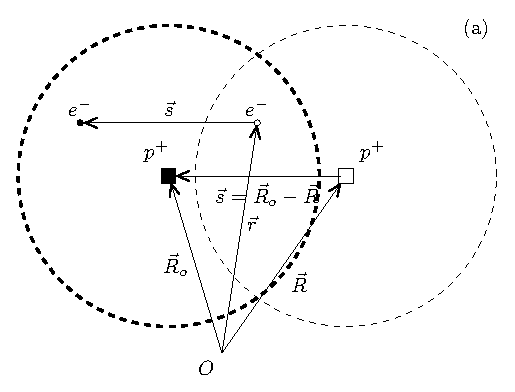
\includegraphics[width=0.49\textwidth]{fig1a}
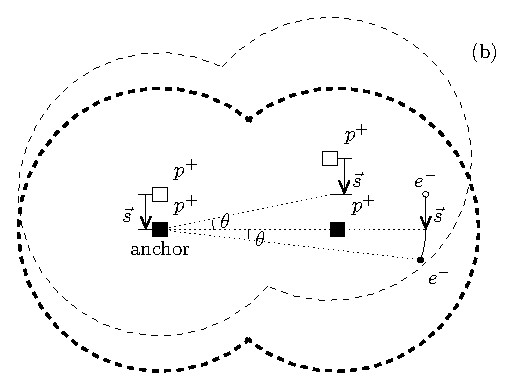
\includegraphics[width=0.49\textwidth]{fig1b}
\caption{Dragged-node approach for simulation of atomic and molecular systems in QMC. {\bf (a)} For atomic systems we can consider the entire wave function shifting with the ion. This process can be visualized by following a contour of the wave function. The thick dashed circle represents a contour of the electronic wave function when the proton is at its reference position $\vec{R}_o$, and the thin dashed circle represents the same contour when the proton has moved to a new position $\vec{R}$. To evaluate the ion-dependent electronic wave function $\bar{\psi}_e(\vec{r},\vec{R})$, we simply map the electron to its proper place in the reference wave function $\psi_e(\vec{r};\vec{R}_o)$. That is, $\bar{\psi}_e(\vec{r},\vec{R})=\bar{\psi}_e(\vec{r}+\vec{s},\vec{R}_o)=\psi_e(\vec{r}+\vec{s};\vec{R}_o)$ where $\vec{s}$ is the shift required to put the proton back to its reference position. {\bf (b)} For H$_2^+$, we pick one of the protons as an ``anchor'' and approximate the new wave function by dragging the reference wave function with the ``anchor'' proton. We also rotate the wave function to align its axis of symmetry with the orientation of the two protons. \label{fig:drag}}
\end{figure}

\subsection{Electron-Ion Wave Function}

Once a satisfactory electronic wave function has been obtained, we construct the electron-ion wave function using the ansatz,
\begin{align}
\Psi_{eI}(\vec{r},\vec{R})=\psi_I(\vec{R})\bar{\psi}_e(\vec{r},\vec{R}), \label{eq:psi}
\end{align}
where $\vec{R}$ denotes the spatial coordinates of all ions and $\bar{\psi}_e(\vec{r},\vec{R})$ is an ion-dependent electronic wave function adapted from the clamped-nuclei wave function $\psi_e(\vec{r};\vec{R}_o)$ through basis set dependence. Due to the localization of Gaussian basis sets around nuclei, as used in quantum chemistry calculations, the nodes of $\bar{\psi}_e$ change based on the ionic positions, which we have previously called the dragged-node approximation.~\cite{Tubman_ECG}
%In general, the nodes only coincide with those obtained in the clamped-ion limit when the ions are at their equilibrium positions $\bar{\psi}_e(\vec{r},\vec{R}_o)=\psi_e(\vec{r};\vec{R}_o)$. However, for atoms and ions this approximation is equivalent to re-optimizing the electronic wave function at each ionic configuration, i.e. $\bar{\psi}_e(\vec{r},\vec{R})=\psi_e(\vec{r};\vec{R})$. 
Although there are approaches for going beyond the dragged-node approximation, it was demonstrated to be highly accurate over a range of molecules in previous work.~\cite{Tubman_ECG} For the systems considered here, we can impose various symmetries of the Hamiltonian onto the wave function that arise from the relative motion of the ions. In Fig.~\ref{fig:drag} we demonstrate this approach for the simple cases of a hydrogen atom and an H$_2^+$ molecular ion. This approach can be generalized for use in larger systems or even applied to parts of a bigger system, e.g., treating light ions as quantum particles and heavy ions as ``clamped".

The term $\psi_I$ consists of simple products of Gaussian wave functions over each pair of nuclei,
\begin{align}
\psi_I(\vec{R})\propto \prod\limits_{i,j>i}e^{-a_{ij}(\vert \vec{R}_i-\vec{R}_j\vert-b_{ij})^2},
\label{wfs_ions}
\end{align}
where $a_{ij}$ is a coefficient that is optimized and $b_{ij}$ are taken to be the equilibrium distances between the nuclei. Since $\psi_I$ is nodeless, the choice of the variational parameters $a_{ij}$ and $b_{ij}$ does not affect the converged FN-DMC energy. FN-DMC is then performed with the fully optimized electron-ion wave function. We perform timestep extrapolation for all of the tested systems. At least four timesteps from $0.005~\text{Ha}^{-1}$ to $0.0005~\text{Ha}^{-1}$ are used for all systems studied in the clamped-nuclei FN-DMC calculation, and at least three timesteps from $0.005~\text{Ha}^{-1}$ to $0.0001~\text{Ha}^{-1}$ are used in the nonadiabatic FN-DMC calculation.

Using definitions from Ref.~\cite{Cederbaum_Review}, the adiabatic approximation will refer to the complete neglect of the nonadiabatic coupling matrix when the Schr$\ddot{\text{o}}$dinger equation is expressed in the basis of eigenstates of the electronic Hamiltonian. In this context, the nonadiabatic contribution to an eigenvalue of the electronic Hamiltonian can be partitioned into two parts: the diagonal Born-Oppenheimer correction (DBOC), which involves only the single electronic state of interest, and the remaining corrections arising from terms that involve excited eigenstates of the electronic Hamiltonian. The DBOC discussed in this work is the expectation value of the nuclear kinetic energy operator in the ground adiabatic electronic state. We define the clamped-nuclei ground-state energy $E_c$ as the lowest eigenvalue of the electronic Hamiltonian and the nonadiabatic ground-state energy $E_n$ as the lowest eigenvalue of the full molecular Hamiltonian that includes the nuclear kinetic energy operator. The zero-point energy (ZPE) for a diatomic molecule is the energy of the ground vibrational state of the one-dimensional vibrational mode. Note that the ZPE of the nuclei is part of the difference $E_n-E_c$. The ZPE is not considered to be nonadiabatic, but its contribution is included in the full molecular Hamiltonian.

\section{Results and Discussion}
\begin{table*}[t!]
\setlength{\extrarowheight}{1pt}
\begin{threeparttable}

\caption{Ground-state energies for atoms and ions and the ionization energies for the atoms:  fixed-node DMC results of this work (FN-DMC) for atoms and ions with and without the Born-Oppenheimer approximation. The rows marked with bold \textbf{FN-DMC} are our nonadiabatic results. The ionization potentials (IPs) are reported in the last section of the table. Energies are given in units of Hartree. For the highly accurate Hylleraas and ECG results, up to 8 digits are reported in the table. \label{tab:ionization}}
\small
\begin{tabular}
% siunitx setup
{
 l
 S[table-format=1.6]
 S[table-format=5.6]
 S[table-format=5.6]
 S[table-format=4.6]
 S[table-format=4.6]
 S[table-format=4.6]
 S[table-format=4.6]
 S[table-format=4.6]
}

\hline\hline
\multicolumn{1}{c}{Atom} & 
\multicolumn{1}{c}{Li$(^2$S)} &
\multicolumn{1}{c}{Be$(^1$S)} &
\multicolumn{1}{c}{B$(^2$P)} &
\multicolumn{1}{c}{C$(^3$P)} &
\multicolumn{1}{c}{N$(^4$S)} &
\multicolumn{1}{c}{O$(^3$P)} &
\multicolumn{1}{c}{F$(^2$P)} \\ 
\hline
\multicolumn{1}{c}{} & 
\multicolumn{1}{c}{} &
\multicolumn{1}{c}{} &
\multicolumn{1}{c}{clamped-ion} &
\multicolumn{1}{c}{} &
\multicolumn{1}{c}{} &
\multicolumn{1}{c}{} &
\multicolumn{1}{c}{} \\
FN-DMC & \text{-}7.478057(5) & \text{-}14.66731(1) & \text{-}24.65374(2) & \text{-}37.84448(2) & \text{-}54.58851(6) & \text{-}75.0658(2) & \text{-}99.73177(6) \\
Seth DMC \cite{Seth_Bench} & \text{-}7.478067(5) & \text{-}14.667306(7) & \text{-}24.65379(3) & \text{-}37.84446(6) & \text{-}54.58867(8) & \text{-}75.0654(1) & \text{-}99.7318(1) \\
$E_{\text{ref}}$\tnote{a} &  \text{-}7.4780603 & \text{-}14.667356 & \text{-}24.653866 & \text{-}37.8450 & \text{-}54.5892 & \text{-}75.0673 & \text{-}99.7339 \\
\multicolumn{1}{c}{} & 
\multicolumn{1}{c}{} &
\multicolumn{1}{c}{} &
\multicolumn{1}{c}{nonadiabatic} &
\multicolumn{1}{c}{} &
\multicolumn{1}{c}{} &
\multicolumn{1}{c}{} &
\multicolumn{1}{c}{} \\
\textbf{FN-DMC} & \text{-}7.47742(2) & \text{-}14.66643(3) & \text{-}24.65252(4) & \text{-}37.84273(4) & \text{-}54.58641(5) & \text{-}75.06313(6) & \text{-}99.7293(1) \\
ECG \tnote{b} & \text{-}7.4774519 & \text{-}14.666435 & \text{-}24.652624 & \text{-}37.841621 & N/A & N/A & N/A \\
\hline

\multicolumn{1}{c}{Ion} & 
\multicolumn{1}{c}{$\text{Li}^+(^1$S)} &
\multicolumn{1}{c}{$\text{Be}^+(^2$S)} &
\multicolumn{1}{c}{$\text{B}^+(^1$S)} &
\multicolumn{1}{c}{$\text{C}^+(^2$P)} &
\multicolumn{1}{c}{$\text{N}^+(^4$S)} &
\multicolumn{1}{c}{$\text{O}^+(^3$P)} &
\multicolumn{1}{c}{$\text{F}^+(^2$P)} \\ 
\hline
\multicolumn{1}{c}{} & 
\multicolumn{1}{c}{} &
\multicolumn{1}{c}{} &
\multicolumn{1}{c}{clamped-ion} &
\multicolumn{1}{c}{} &
\multicolumn{1}{c}{} &
\multicolumn{1}{c}{} &
\multicolumn{1}{c}{} \\
FN-DMC & \text{-}7.27989(2) & \text{-}14.324749(7) & \text{-}24.34883(1) & \text{-}37.43071(2) & \text{-}54.05371(5) & \text{-}74.56597(6) & \text{-}99.0909(1) \\
Seth DMC \cite{Seth_Bench} & \text{-}7.279914(3) & \text{-}14.324761(3) & \text{-}24.34887(2) & \text{-}37.43073(4) & \text{-}54.05383(7) & \text{-}74.56662(7) & \text{-}99.0911(2) \\
$E_{\text{ref}}$\tnote{c} & \text{-}7.2799134 & \text{-}14.324763 & \text{-}24.348884 & \text{-}37.430880 & \text{-}54.0546 & \text{-}74.5668 & \text{-}99.0928 \\ 
\multicolumn{1}{c}{} &
\multicolumn{1}{c}{} &
\multicolumn{1}{c}{} &
\multicolumn{1}{c}{nonadiabatic} &
\multicolumn{1}{c}{} &
\multicolumn{1}{c}{} &
\multicolumn{1}{c}{} &
\multicolumn{1}{c}{} \\
\textbf{FN-DMC} & \text{-}7.27931(4) & \text{-}14.32387(2) & \text{-}24.34758(3) & \text{-}37.42899(6) & \text{-}54.05165(4) & \text{-}74.5634(1) & \text{-}99.0885(1) \\
ECG \tnote{d} & N/A &  \text{-}14.323863 &  \text{-}24.347641 &  \text{-}37.429169 & N/A & N/A & N/A \\
\hline
\multicolumn{1}{c}{} & 
\multicolumn{1}{c}{} &
\multicolumn{1}{c}{} &
\multicolumn{1}{c}{clamped-ion} &
\multicolumn{1}{c}{} &
\multicolumn{1}{c}{} &
\multicolumn{1}{c}{} &
\multicolumn{1}{c}{} \\
IP (FN-DMC) & 0.19817(2) & 0.34256(1) & 0.30490(2) & 0.41377(3) & 0.53479(8) & 0.4998(2) & 0.6409(1) \\
\multicolumn{1}{c}{} & 
\multicolumn{1}{c}{} &
\multicolumn{1}{c}{} &
\multicolumn{1}{c}{nonadiabatic} &
\multicolumn{1}{c}{} &
\multicolumn{1}{c}{} &
\multicolumn{1}{c}{} &
\multicolumn{1}{c}{} \\
IP (\textbf{FN-DMC}) & 0.19811(4) & 0.34257(4) & 0.30494(5) & 0.41374(7) & 0.53476(7) & 0.4998(1) & 0.6408(1) \\
IP (Ref.)\tnote{e} & 0.198130 & 0.342572 & 0.304980 & 0.414014 & 0.534775 & 0.500452 & 0.640946 \\
\hline\hline
\end{tabular}

\begin{tablenotes}
\item[a] For the atomic references, we use the Hylleraas result for Li,~\cite{Wang_Li} and ECG results for Be~\cite{Stanke_Be} and B.~\cite{Bubin_B} Ref.~\cite{Davidson_Atoms} is used for C,N,O and F where the ground-state energies are taken from Table XI.
\item[b] We use nonadiabatic ECG results as the reference for Li,~\cite{Stanke_Li} Be~\cite{Bubin_BeH_noBO} and B~\cite{Bubin_B}, which are converged to the true ground-state to well within 0.1 mHa. The result for C,~\cite{Bubin_C} however, may have error on the order of 1 mHa.
\item[c] For the ionic references, we use the ICI result for $\text{Li}^+$,~\cite{Nakashima_Li+} Hylleraas result for $\text{Be}^+$~\cite{Puchalski_Be} and ECG results for $\text{B}^+$~\cite{Bubin_B+} and $\text{C}^+$.~\cite{Bubin_C+,mitroy2013} Ref.~\cite{Davidson_Atoms} is used for $\text{N}^+$,$\text{O}^+$,$\text{F}^+$.
\item[d] ECG references only exist for $\text{Be}^+$,~\cite{Bubin_BeH_noBO} $\text{B}^+$~\cite{Bubin_B+} and $\text{C}^+$.~\cite{Bubin_C+}
\item[e] Spin-orbit coupling and relativistic corrections~\cite{Klopper_IP} are removed from experimental data~\cite{NIST_Atoms} for comparison.
\end{tablenotes}

\end{threeparttable}
\end{table*}

\subsection{Atoms and Ions}

To assess the quality of our results for atoms and ions~\footnotemark\footnotetext{All calculations are performed for the most abundant isotope. In units of electron mass, the isotope masses for Li, Be, B, C, N, O, F are taken to be 12782.4327, 16419.2608, 20214.7648
6, 21862.7553, 25512.1484, 29141.0754, 34613.1200, respectively. The Li mass used for the LiH molecule is 12649.6690, which is slightly different from that used for the atomic Li simulations, but we do not expect this to affect our results within our statistical errors.}, we compare to previous results from highly accurate simulations, as presented in Table \ref{tab:ionization}. For the clamped-ion results, QMC~\cite{Brown_Bench,Toulouse_Bench,Seth_Bench,Morale_Bench,Rappe_Bench} and quantum chemistry benchmarks are available for comparison. To illustrate the high-quality QMC techniques used in this work, we compare our clamped-ion atomic results with a recent QMC benchmark study.~\cite{Seth_Bench} The ground-state FN-DMC energies consistently agree across all systems studied (except for O$^{+}$) within 0.1 mHa. This shows that similar nodes can be obtained with different forms of the wave function. In particular, our large ($\sim$ 1000 CSF) multi-determinant expansions can be compared with the approach used by Seth {\it et al.},~\cite{Seth_Bench} which relies on moderately-sized multi-determinant expansions ($\sim$ 100 CSF) with a backflow transformation. For certain atoms, we can compare to more accurate simulation techniques. For C$^+$ as well as the neutral and ionized Li, Be and B, well-converged ECG calculations are available, where basis set error is converged to less than 0.1 mHa. This convergence is corroborated by results from the Hylleraas method for Li~\cite{Wang_Li} and Be$^+$.~\cite{Puchalski_Be} In Table \ref{tab:ionization}, we have used the lowest variational results as our references for these systems, as the convergence is such that the accuracy is higher than other current theoretical or experimental estimates. 

All of our clamped-ion results agree within 0.2 mHa of the ECG references, as shown in Figure \ref{fig:atom-ECG}. The error bars for the reference ECG results are absorbed into the DMC error bars for clarity, because the ECG error bars are orders of magnitude smaller compared to the DMC error bars. While ECG results exist for C and N, they are not well converged and are not suitable references.~\cite{Bubin_C,Sharkey_N} The benchmark results in Ref.~\cite{Davidson_Atoms} are a standard for atomic energies, and we report them as our references in Table \ref{tab:ionization} for the larger atoms. However, these benchmark results are not consistently accurate to 0.1 mHa. For instance, if we use the ECG results for $\text{C}^+$ with the most accurate ionization reference energy, then we find a reference energy for the C atom of -37.84489 Ha, which is 0.1 mHa higher than that reported in Ref.~\cite{Davidson_Atoms}. %Nevertheless, a comparison of our results with the references suggests that our ground-state energies for the neutral and ionized N,O,F are not accurate to the sub mHa level. 
The systems with the most error are O and F, for which other QMC studies seem to experience similar difficulties.~\cite{Seth_Bench,Booth_FCIQMC,Brown_Bench,Shiwei_AFQMC} We note that for some of these systems it may be possible to absorb the sign problem and increase the accuracy further in future studies.~\cite{Tubman_Release,Tubman_ACS} %However, a systematic exploration of these alternatives is beyond the scope of the current study.

\begin{figure}[h]
\centering
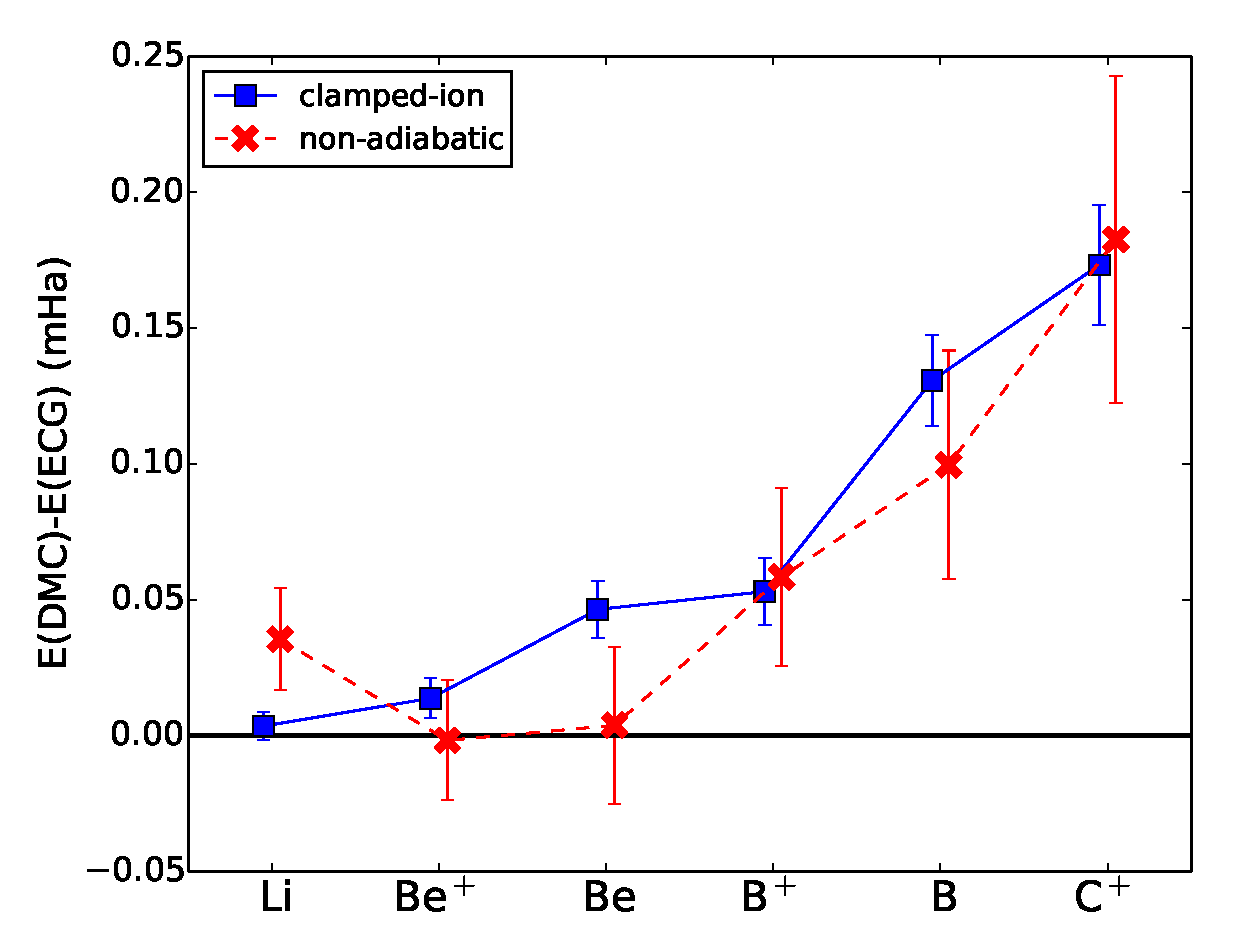
\includegraphics[width=0.8\textwidth]{atom-ECG}
\caption{FN-DMC ground state energies for $\text{Be}^+$, Be, $\text{B}^+$, B, $\text{C}^+$ relative to ECG references~\cite{Stanke_Be,Puchalski_Be,Bubin_BeH_noBO,Bubin_B,Bubin_B+,Bubin_C+} for either clamped-ion or nonadiabatic calculations. These relative energies provide an estimate for the fixed-node error in the electronic and electron-ion wave functions, respectively.\label{fig:atom-ECG}}
\end{figure}

It is more difficult to find accurate references for the nonadiabatic results. We provide the first nonadiabatic QMC benchmarks for the first-row atoms. There are six ECG calculations of nonadiabatic ground-state energies that are reportedly converged beyond 0.1 mHa, which we use as references. Our reported nonadiabatic ground-state energies for Li, Be, $\text{Be}^+$, B, $\text{B}^+$ and $\text{C}^+$ are in agreement with the ECG results to within 0.2 mHa, as shown in Figure \ref{fig:atom-ECG}. For these systems, the ECG results are converged to essentially the exact ground-state energies in both the clamped-ion and nonadiabatic cases. The difference between our DMC ground-state and ECG reference is the fixed-node error present in our wave functions. We would expect the clamped ion results to be more accurate than the nonadiabatic results, since the nonadiabatic wave functions are inherently more difficult to construct.  However, for the systems in Figure \ref{fig:atom-ECG}, this difference in quality is less than 0.1 mHa.
%In the case of Be, $\text{Be}^+$, and B,  the nonadiabatic wave function is actually more accurate than the corresponding clamped-ion wave function.

No reference calculations exist for the heavier atoms N, O, and F. However, it is possible to apply finite-mass correction~\cite{Davidson_Atoms,Cencek_LiH} (i.e., divide by $1+m_e/M$, where $m_e$ is the mass of an electron and $M$ is the mass of the nucleus) to the best clamped-ion references to estimate the nonadiabatic references. The energies for N, O, and F obtained in this way are -54.5871, -75.0647 and -99.7310 Ha, respectively. For the ionized states, we obtain -54.0525, -74.5643 and -99.0900 Ha. %A comparison of our results to these references reveals that the electronic and electron-ion wave functions are of similar quality for all atoms and ions. %Notice the fixed-node error is virtually identical in the electronic wave function and electron-ion wave function of the same system, suggesting that our approach is capable of generating high quality electron-ion wave function from an optimized electronic wave function.

\begin{figure}[h]
\centering
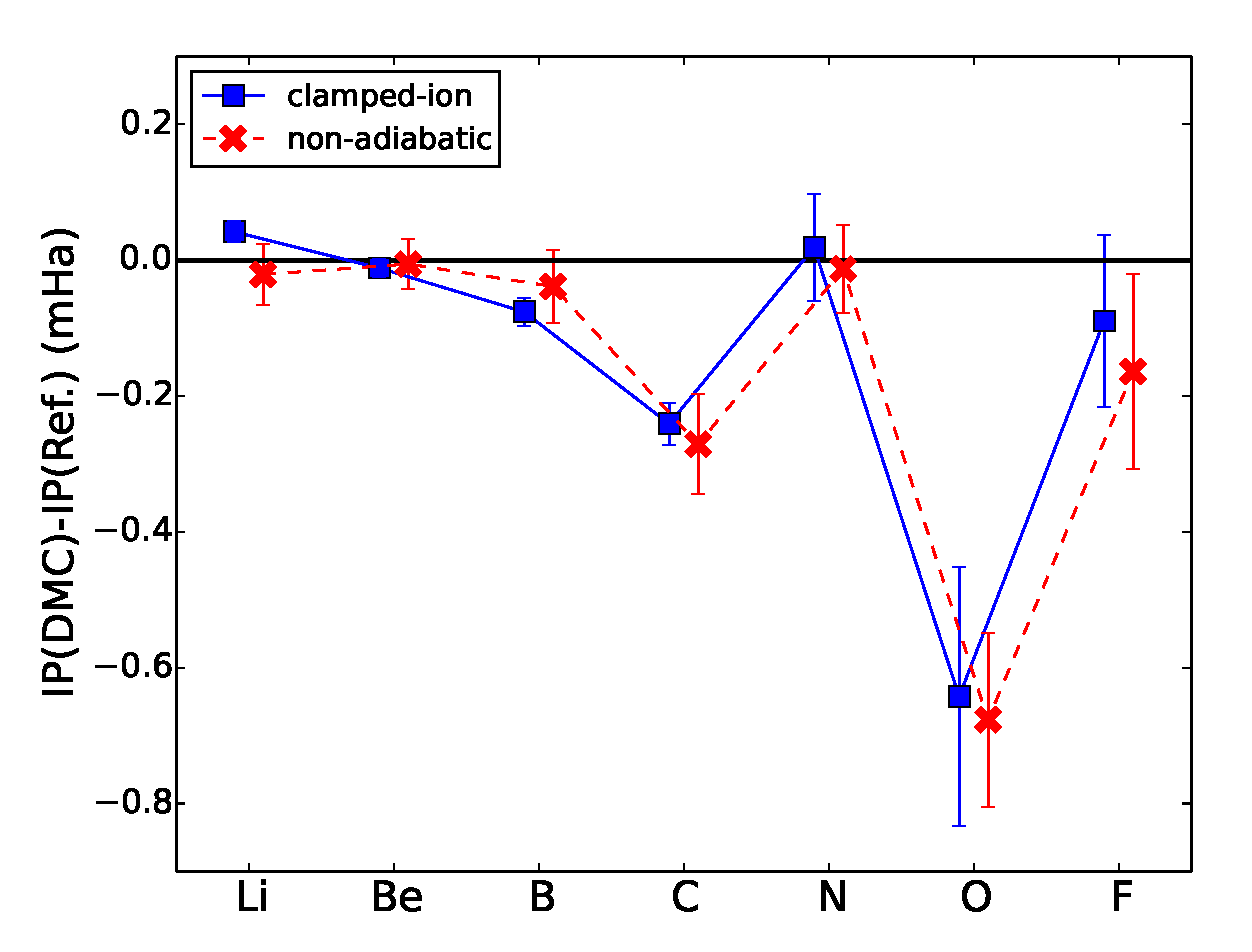
\includegraphics[width=0.8\textwidth]{ionization}
\caption{Calculated ionization energies relative to reference data. The same reference is used for both clamped-ion and nonadiabatic results. The calculated energies are all within 1 mHa of the reference. \label{fig:ionization}}
\end{figure}

The ionization potentials are reported in Table \ref{tab:ionization} and shown in Figure \ref{fig:ionization}. For determining a set of nonadiabatic reference data, we subtract the spin-orbit and relativistic corrections (estimated by Klopper et. al.~\cite{Klopper_IP}) from the NIST experimental data.~\cite{NIST_Atoms} Ref.~\cite{Klopper_IP} is considered to have the most accurate ionization energies due to its usage of state-of-the-art quantum chemistry techniques shown to provide close agreement with experiment.
%We believe these are more accurate than another widely used reference~\cite{Davidson_Atoms} because the latter estimates ionization potentials in the infinite-nucleus-mass limit, and the former uses corrections from state-of-the-art quantum chemistry techniques. However, the differences between the two references are only significant for obtaining benchmarks better than 0.5 mHa. 
For the atoms considered in this work, ionization energies have previously been predicted to be independent of all nonadiabatic effects beyond the DBOC to within an accuracy of 0.1 mHa.~\cite{Klopper_IP} This prediction is based on calculations that are reported to be exact and agree to high accuracy with experiment. As shown in Figure \ref{fig:ionization}, the ionization potentials calculated with and without the Born-Oppenheimer approximation are all within 1 mHa of the reference energies. Further, the clamped-ion and nonadiabatic predictions for the ionization potentials are statistically indistinguishable for all systems studied, consistent with the previous study.~\cite{Klopper_IP}

\begin{figure}[h]
\centering
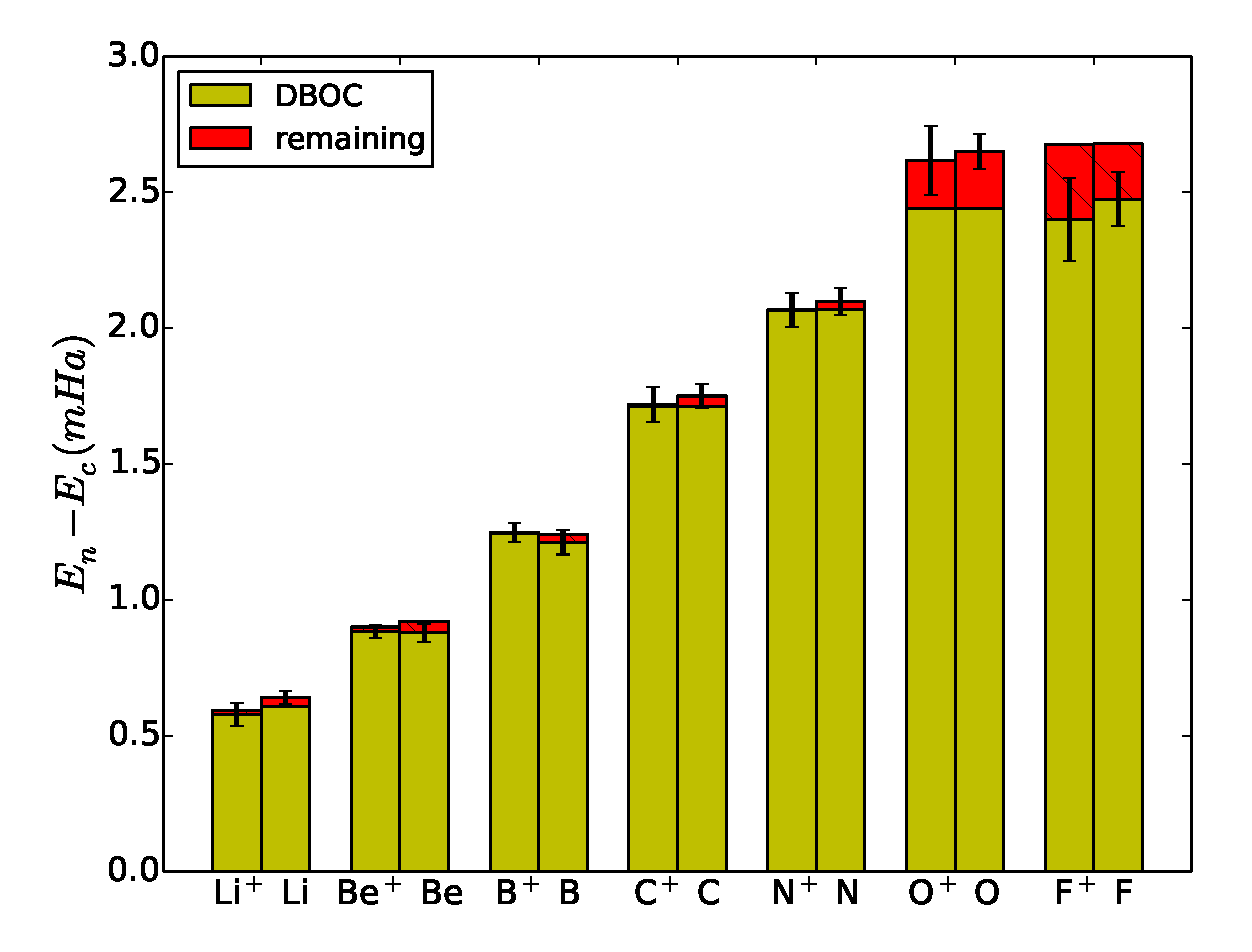
\includegraphics[width=0.8\textwidth]{atom-nad-ad}
\caption{The nonadiabatic contribution to ground-state energies of atoms and ions calculated with FN-DMC. The nonadiabatic contribution is partitioned into the DBOC and the remaining correction. A hatched bar indicates the contribution is negative. The numerical DBOC data is provided in Table \ref{tab:nad-ad-atoms}. \label{fig:atom-nad-ad}} %nonadiabatic contribution shows very little dependence with the ionized state.
\end{figure}

\begin{figure}[h]
\centering
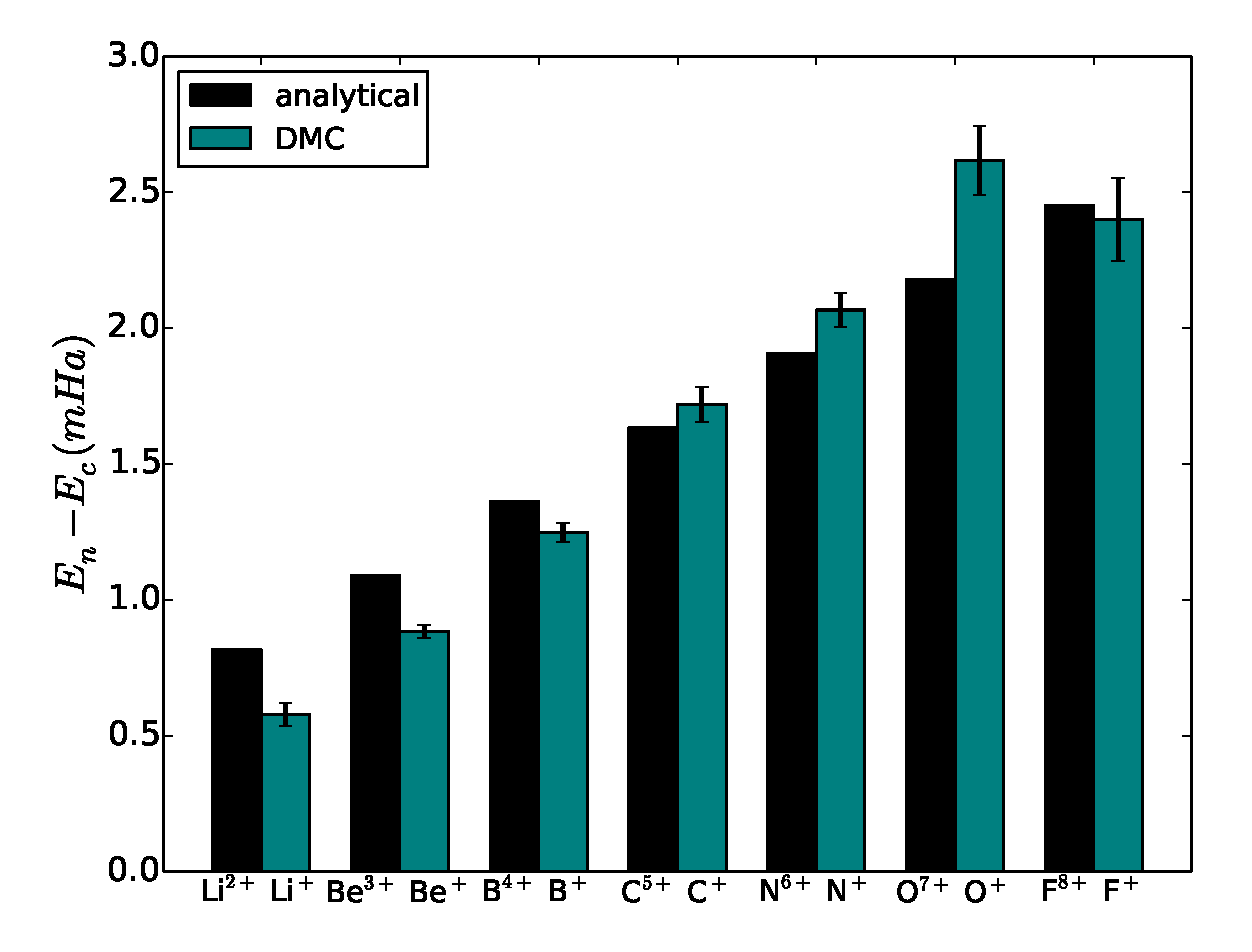
\includegraphics[width=0.8\textwidth]{analytical}
\caption{The nonadiabatic contribution to ground-state energies of ions and their corresponding hydrogen-like atoms calculated with FN-DMC and analytically as shown in Eq. \ref{eq:analytical}. \label{fig:analytical}}
\end{figure}

\begin{table}[h]
\centering
\setlength{\extrarowheight}{1pt}
\caption{Nonadiabatic corrections for the ground-state energies of atoms and ions. $E_n$ and $E_c$ are the FN-DMC calculations of the nonadiabatic and clamped ground-state energies, respectively. The DBOC contribution is provided by Wim Klopper (personal communication). All energies are reported in units of mHa.\label{tab:nad-ad-atoms}}
\begin{tabular}{ccc|ccc}
\hline\hline
System & $E_n-E_c$&  DBOC     & System & $E_n-E_c$&  DBOC \\ \hline
Li$^+$ &   0.58(4) &  0.591970 & Li     &   0.64(2) &  0.608411 \\
Be$^+$ &   0.88(2) &  0.899706 & Be     &   0.88(3) &  0.920848 \\
B$^+$  &   1.25(4) &  1.242988 & B      &   1.21(5) &  1.241669 \\
C$^+$  &   1.72(6) &  1.710382 & C      &   1.75(5) &  1.710900 \\
N$^+$  &   2.07(6) &  2.066914 & N      &   2.10(8) &  2.069149 \\
O$^+$  &   2.6(1) &  2.440320  & O      &   2.6(2)&  2.441821 \\
F$^+$  &   2.4(2) &  2.675128  & F      &   2.5(1)&  2.678181 \\
\hline\hline
\end{tabular}
\end{table}


In Table \ref{tab:nad-ad-atoms} and Figure \ref{fig:atom-nad-ad}, we demonstrate the amount of nonadiabatic contribution to the ground-state energies in atoms and ions calculated as the difference between the nonadiabatic and clamped-ion ground-state energies. The amount of nonadiabatic contribution is always positive for these systems and mostly increases with atomic number. Using previous benchmark values for the DBOC, we can break down the nonadiabatic contribution of our system into a DBOC contribution and everything beyond the DBOC.\footnotemark\footnotetext{The DBOC values for the atoms and ions provided by Prof. Wim Klopper are calculated at the CCSD/d-aug-cc-pwCVQZ level using CFOUR.}\footnotemark\footnotetext{CFOUR, a quantum chemical program package written by J.F. Stanton, J. Gauss, M.E. Harding, P.G. Szalay and others.}~\cite{Harding} The DBOC is relatively insensitive to the level of theory. Figure \ref{fig:atom-nad-ad} indicates that in the atomic systems, the DBOC is the dominant contribution to the nonadiabatic energy, with the remaining amount being close to zero within error bars. The nonadiabatic energy is relatively constant between the neutral and cationic species. This observation suggests that the amount of nonadiabatic contribution is insensitive to the addition or removal of a valence electron. Physically, the valence electrons are farther from the nucleus than the core electrons, thus are likely to be affected to a lesser degree by the delocalization of the nucleus. 

The nonadiabatic contributions in the cations can also be compared with those in their corresponding hydrogen-like atoms for a more in-depth analysis. The nonadiabatic contribution in a hydrogen-like atom can be obtained analytically. The result in Hartree atomic units is
\begin{align}
E_n-E_c=\frac{Z^2}{2}(1-\mu) \label{eq:analytical}
\end{align}
where $\mu=\frac{M}{M+1}$ is the reduced mass of the hydrogen-like atom and $M$ and $Z$ are the mass and atomic number of the nucleus, respectively. The increase in the nonadiabatic contribution with increasing $Z$ for hydrogen-like atoms reflects the stronger Coulombic attraction between the electron and the nucleus, which enhances the effects of the delocalization of the nucleus. An interesting case to consider is the transition from Li$^{2+}$ to Li. As shown in Figure \ref{fig:atom-nad-ad} and Figure \ref{fig:analytical}, the addition of a core electron to Li$^{2+}$ decreases the nonadiabatic contribution, while the addition of a valence electron has no further effect within our error bars. We also calculate the nonadiabatic contribution in Be$^{2+}$ to be $0.78(5)$ mHa, which is $0.29(5)$ mHa lower than the nonadiabatic contribution in Be$^{3+}$ and is closer to that in Be$^{+}$ of 0.88(2) mHa. Because the core electrons interact more strongly with the nucleus than do the valence electrons, the core electrons are affected more by the delocalization of the nucleus. Moreover, the addition of a second core electron decreases the nonadiabatic contribution for Li$^{2+}$ and Be$^{3+}$. %due to correlation with the first core electron.%shielding effects.
We note that the nonadiabatic correction to the atomic ground-state energies of Eq. (\ref{eq:analytical}), which only holds for single electron systems, is roughly linear in Z, while the relativistic recoil correction~\cite{Merkt_H2} scales as $Z^4$. Therefore, the nonadiabatic effect is not seen experimentally,  as it is less significant than this relativistic effect.

\subsection{Hydrides}

\begin{sidewaystable*}[t!]
\setlength{\extrarowheight}{1pt}
\begin{threeparttable}
\caption{Ground-state energies and atomization energies: fixed-node DMC results of this work for all first row hydrides with and without the Born-Oppenheimer approximation. The rows marked with bold \textbf{FN-DMC} are our nonadiabatic results. All atomization energies are estimated for 0K. $D_o$ includes zero-point energy contribution, while $D_e$ does not. Both total energies and dissociation energies are given in units of Hartree. \label{tab:atomization}}
\begin{tabular}
% siunitx setup
{
 l
 S[table-format=1.6]
 S[table-format=4.6]
 S[table-format=4.6]
 S[table-format=4.6]
 S[table-format=4.6]
 S[table-format=4.6]
 S[table-format=4.6]
}

\hline\hline
\multicolumn{1}{c}{Molecule} & 
\multicolumn{1}{c}{LiH$(^1\Sigma^+)$} &
\multicolumn{1}{c}{BeH$(^2\Sigma^+)$} &
\multicolumn{1}{c}{BH$(^1\Sigma^+)$} &
\multicolumn{1}{c}{CH$(^2\Pi)$} &
\multicolumn{1}{c}{OH$(^2\Pi)$} &
\multicolumn{1}{c}{HF$(^1\Sigma^+)$} \\ 
\hline
\multicolumn{1}{c}{} & 
\multicolumn{1}{c}{} &
\multicolumn{1}{c}{} &
\multicolumn{1}{c}{clamped-nuclei} &
\multicolumn{1}{c}{} &
\multicolumn{1}{c}{} &
\multicolumn{1}{c}{} \\
FN-DMC & \text{-}8.070518(7) & \text{-}15.24793(2) & \text{-}25.28867(3) & \text{-}38.4780(1) & \text{-}75.7356(1) & \text{-}100.4552(1) \\
$E_{\text{ref}}$ \tnote{a} & \text{-}8.0705473 & \text{-}15.2483(4) & \text{-}25.2893(2) & \text{-}38.4792(2) & \text{-}75.7382(2) & \text{-}100.4600(3) \\
\multicolumn{1}{c}{} & 
\multicolumn{1}{c}{} &
\multicolumn{1}{c}{} &
\multicolumn{1}{c}{nonadiabatic} &
\multicolumn{1}{c}{} &
\multicolumn{1}{c}{} &
\multicolumn{1}{c}{} \\
\textbf{FN-DMC} & \text{-}8.06624(3) & \text{-}15.24194(5) & \text{-}25.28128(9) & \text{-}38.4672(3) & \text{-}75.7245(5) & \text{-}100.4431(4) \\
ECG \cite{Bubin_LiH_noBO,Bubin_BeH_noBO,Bubin_BH_noBO} & \text{-}8.0664371(15) & \text{-}15.24203(10) & \text{-}25.2803(10) & N/A & N/A & N/A \\
\hline

\multicolumn{1}{c}{} & 
\multicolumn{1}{c}{} &
\multicolumn{1}{c}{} &
\multicolumn{1}{c}{clamped-nuclei} &
\multicolumn{1}{c}{} &
\multicolumn{1}{c}{} &
\multicolumn{1}{c}{} \\
$D_e$ (FN-DMC) & 0.09246(1) & 0.08062(2) & 0.13493(3) & 0.1335(1) & 0.1699(2) & 0.2234(1) \\
$D_e$ Feller \tnote{b} & 0.09262(5) & 0.0809(4) & 0.1354(2) & 0.1342(2) & 0.1709(2) & 0.2258(3) \\
\multicolumn{1}{c}{} & 
\multicolumn{1}{c}{} &
\multicolumn{1}{c}{} &
\multicolumn{1}{c}{nonadiabatic} &
\multicolumn{1}{c}{} &
\multicolumn{1}{c}{} &
\multicolumn{1}{c}{} \\
$D_o$ (\textbf{FN-DMC}) & 0.08910(4)  & 0.07578(6)  & 0.1290(1) & 0.1248(3) & 0.1617(5) & 0.2141(4) \\
$D_o$ Feller \tnote{c} & 0.08940(5) & 0.0761(4) & 0.1299(2) & 0.1276(2) & 0.1622(2) & 0.2166(3)\\
$D_o$ Exp. \cite{CCCBDB,HH} & 0.08874(38) & 0.07475(4) & 0.1281(37)\tnote{d} & 0.1275(5) & 0.1622(1) & 0.2158(3) \\
\hline\hline
\end{tabular}
\begin{tablenotes}
\item[a] For LiH, ECG provides the best reference energy.~\cite{Adamowicz_LiH} For the rest of the systems, we combined the best clamped-ion atomic references in Table \ref{tab:ionization} and thermochemistry estimates of $D_e$ in this table to produce the reference ground-state energies.
\item[b] Estimates for $D_e$ are calculated by subtracting the scalar relativistic, spin-orbit coupling and zero-point energy corrections from the reference $D_o$ in Table VI of Ref.~\cite{Feller_Corrections}.
\item[c] Here only the scalar relativistic and spin-orbit coupling corrections are subtracted.
\item[d] The atomization energy for BeH in Ref.~\cite{CCCBDB} disagrees with previous high-level theoretical benchmarks,~\cite{Feller_Corrections,Bubin_BeH_noBO} thus we use Ref.~\cite{HH} instead. For several of the systems, multiple experimental values are available in the literature.  We report experimental values that were aggregated in one single reference,~\cite{CCCBDB} except for BeH.~\cite{HH}
\end{tablenotes}
\end{threeparttable}
\end{sidewaystable*}
In Table \ref{tab:atomization}, we present our results on a series of molecular systems (hydrides). Finding accurate reference data for these systems to 0.1 mHa is not straightforward. We will use highly converged ECG data when available. Two ECG calculations have been performed in the clamped-nuclei limit for LiH~\cite{Cencek_LiH,Adamowicz_LiH} and we agree within 0.03 mHa with the more recent reference. For the rest of the systems, we combined the best clamped-ion atomic references in Table \ref{tab:ionization} and thermochemistry~\cite{Feller_Corrections} estimates of atomization energy $D_e$ in Table \ref{tab:atomization} to produce the reference ground-state energies. For BeH and BH, we are within 1 mHa of the reference values, and our energies are lower than the best available quantum chemistry results of -15.247846 Ha~\cite{Koput_BeH} and -25.287650 Ha~\cite{Miliordos_BH} for BeH and BH, respectively. 
%For the rest of the systems it is possible we have the lowest variational estimates. %, but a comparison with reference suggests that we have fixed-node error in the range of a few mHa.

\begin{figure}[h]
\centering
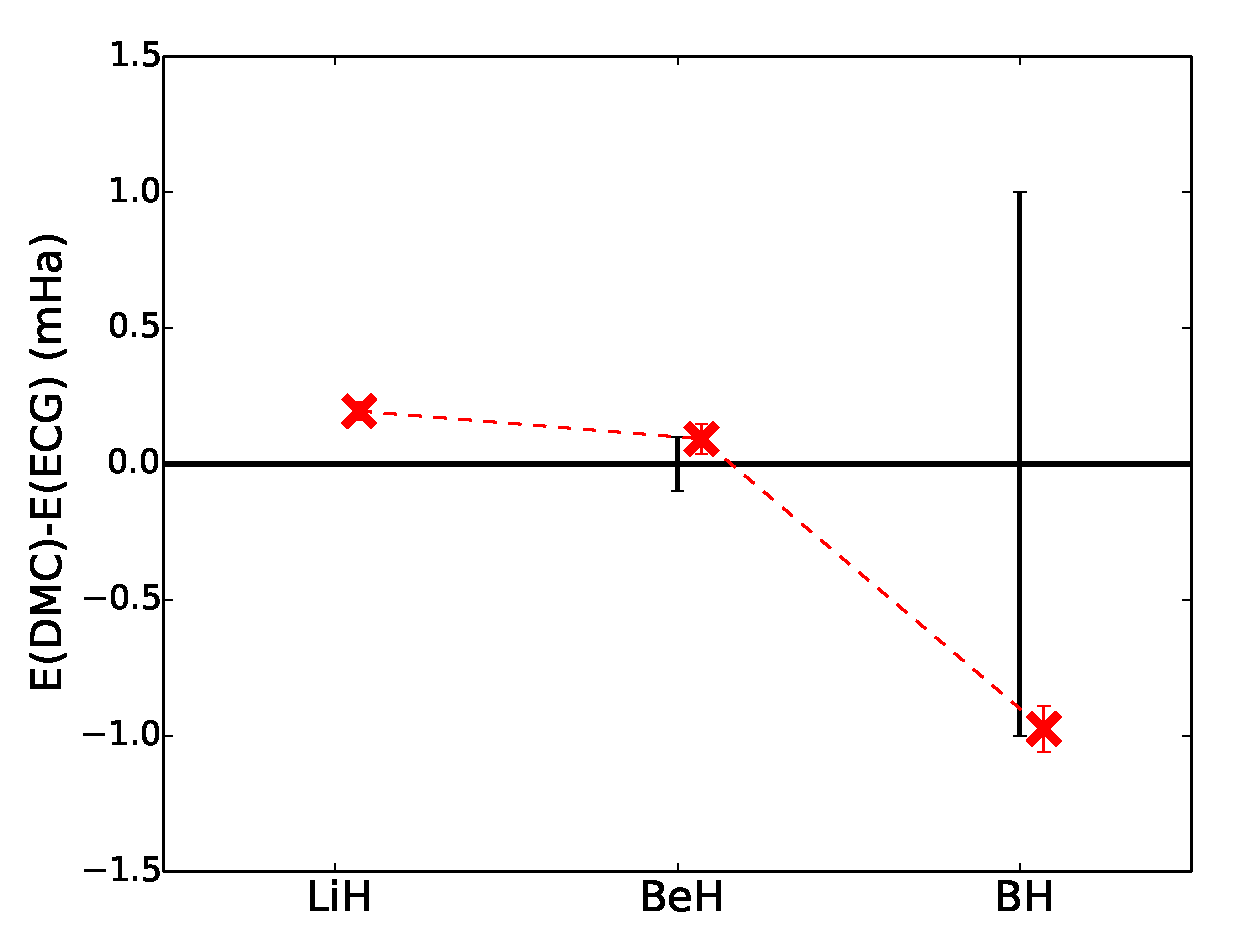
\includegraphics[width=0.8\textwidth]{dia-ECG}
\caption{The nonadiabatic FN-DMC ground-state energies of LiH, BeH and BH relative to ECG references. The error bars for the nonadiabatic ECG references are shown as thick dark lines, and the error bars for the FN-DMC calculations are comparable to the size of the symbols. \label{fig:dia-ECG}}
\end{figure}

Nonadiabatic ECG calculations only exist for the three smallest hydrides. Our results for LiH and BeH agree with the ECG references to within 0.2 mHa, as shown in Figure \ref{fig:dia-ECG}. The ECG reference for LiH is converged to the true ground-state energy beyond 0.1 mHa; thus, it is likely that our wave function has a fixed-node error of 0.2 mHa. For BeH, our result is within 0.1 mHa of the ECG reference and agrees within error bars. With BH being one of the largest ECG simulations performed, the DMC result is actually lower in energy, in this case by 1 mHa. The ECG error bar on BH is large, and it is not evident how close our result is to the true ground state, although extrapolating the ECG result with basis set size suggests we are within 1 mHa.~\cite{Bubin_BeH_noBO} For these nonadiabatic systems, we have the lowest variational result for BH, and the only simulated results of for CH, OH, and HF, to the best of our knowledge.

The atomization energies of the diatomic systems are reported in Table \ref{tab:atomization}. High-quality thermochemistry benchmarks are used for comparison.~\cite{Feller_Corrections} We take the reference energies from the last column of Table VI of Ref.~\cite{Feller_Corrections} and subtract the corrections in the $\Delta E_{SR}$ (scalar relativistic) and SO (spin-orbit coupling) columns for the comparison with our non-relativistic energies. For the comparison with our clamped-nuclei results, we further subtract the DBOC and ZPE (zero-point energy) corrections.
%Corrections from spin-orbit coupling and relativistic effects are not used, as they are not included in our Hamiltonian.
The atomization energies estimated in the clamped-nuclei limit agree within 1 mHa of the references for all but the largest molecule, HF. Within quantum Monte Carlo, it is generally more difficult to obtain an accurate nodal surface for a molecule than for an atom. As a result, our estimates for the clamped-nuclei atomization energies are lower than the references in all cases. A similar trend can be observed when comparing our nonadiabatic results with the references. For each molecule, the deviation from the reference is similar in the clamped-nuclei and nonadiabatic cases except for CH.

\begin{figure}[h]
\centering
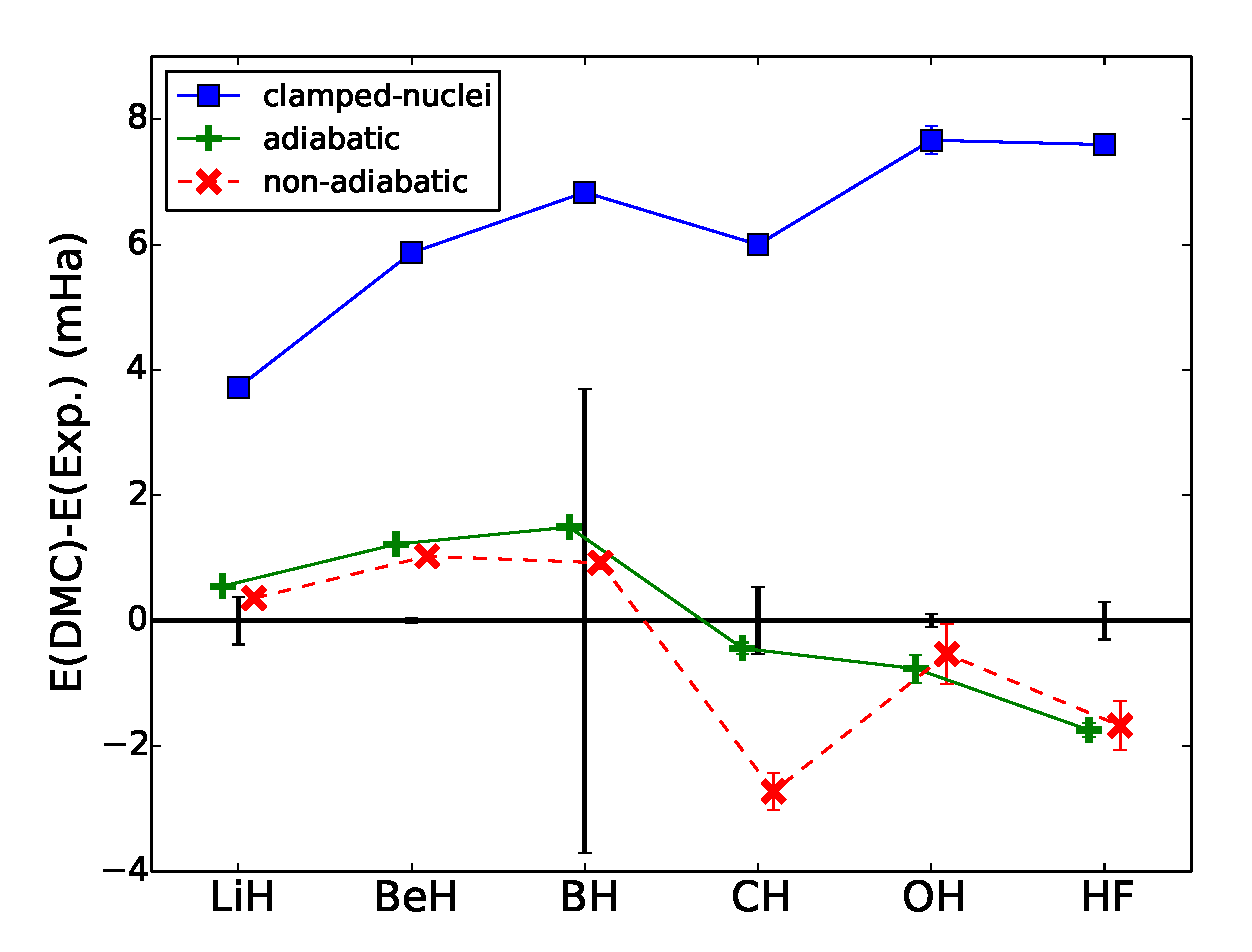
\includegraphics[width=0.8\textwidth]{atomization}
\caption{Atomization energies of first row hydrides obtained with FN-DMC relative to experimental data. The adiabatic results are estimated by adding zero-point energies from Ref.~\cite{Feller_Corrections} to the clamped-nuclei results. \label{fig:atomization}}
\end{figure}

In Figure \ref{fig:atomization}, we compare both our clamped-nuclei and our nonadiabatic results to experimental data. We also provide adiabatic estimates by adding the zero-point energies calculated with coupled-cluster techniques in Ref.~\cite{Feller_Corrections} to our clamped-nuclei results. To calculate experimental atomization energies starting from the clamped-nuclei results, energetic corrections due to zero-point motion of the nuclei, nonadiabatic effects, spin-orbit coupling and relativistic effects should be included. For these highly adiabatic systems, the inclusion of zero-point motion alone is sufficient to bring our clamped-nuclei results to within 2 mHa of the experimental results. Except for the case of CH, the nonadiabatic results agree closely with their adiabatic counterparts and are closer to the experimental values, although for BH the experimental error bar is too large to provide a high-accuracy comparison. For CH, the experimental result suggests that our electron-ion wave function for this molecule has an unusually large fixed-node error.

\begin{figure}[h]
\centering
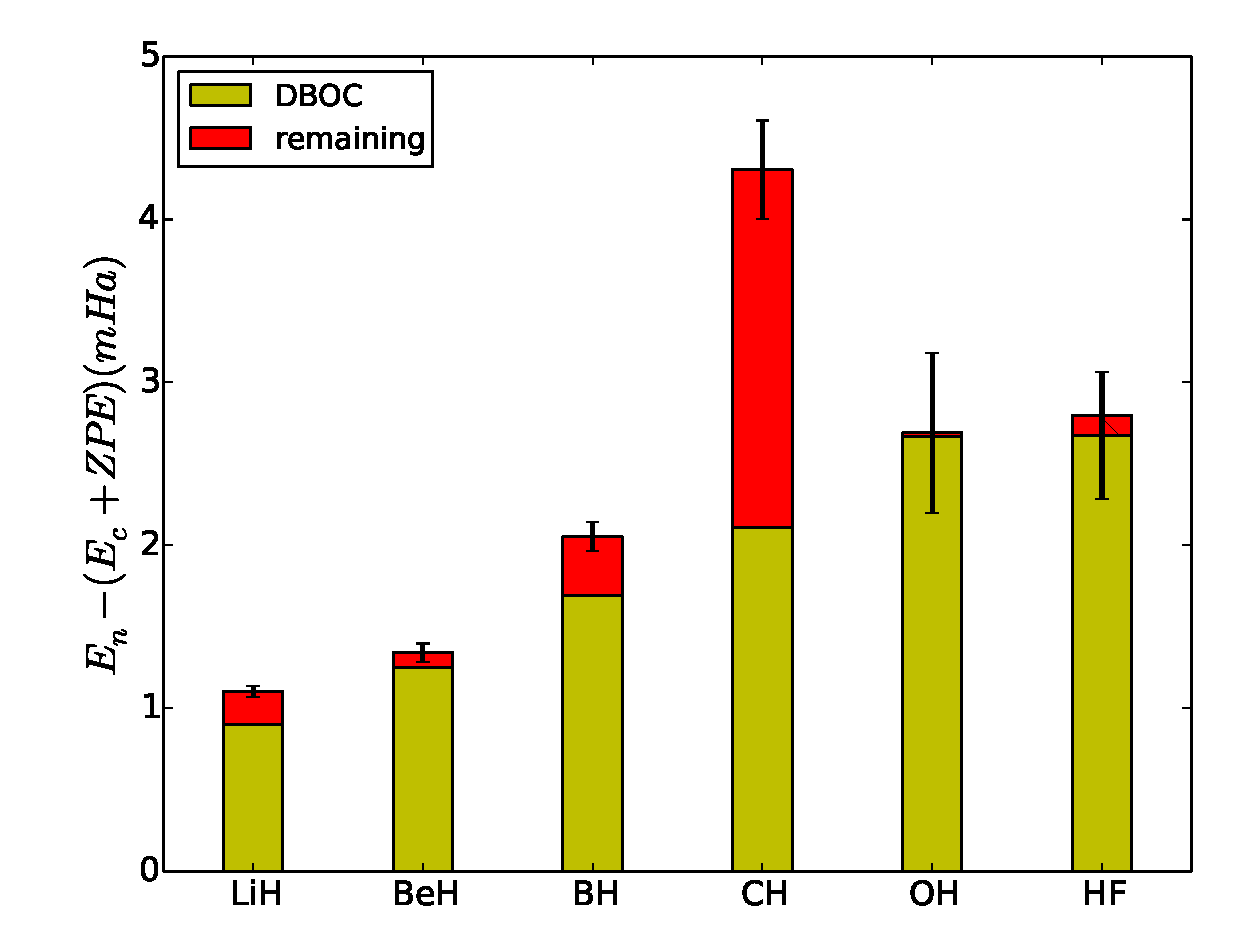
\includegraphics[width=0.8\textwidth]{dia-nad-ad}
\caption{The nonadiabatic contribution to the ground-state energies in hydrides calculated with FN-DMC. The adiabatic reference energies are calculated by adding zero-point energy contributions from Ref.~\cite{Feller_Corrections} to our clamped-nuclei results. The nonadiabatic contribution is partitioned into the DBOC and the remaining correction. A hatched bar indicates the contribution is negative. \label{fig:dia-nad-ad}}
\end{figure}

To estimate the nonadiabatic contribution to the ground-state energies for these hydrides, we calculate the difference between our nonadiabatic and adiabatic results, as shown in Figure \ref{fig:dia-nad-ad}. Similar to the atomic case, we break down the nonadiabatic energy of our system into a DBOC contribution and everything beyond the DBOC.\footnotemark\footnotetext{The DBOC references provided by Prof. David Feller are calculated at the CCSD(T)/aug-cc-pVTZ level using CFOUR}~\cite{Harding} The ZPE and DBOC contributions to this difference are listed in Table \ref{tab:nad-ad-diatomics}. We also calculate the nonadiabatic correction to the dissociation energies of the hydrides.
%The total amount of nonadiabatic contribution appears to peak for CH, although this larger contribution may reflect the larger fixed-node error for this system. 
For BeH, OH, and HF, the nonadiabatic contribution is almost entirely accounted for by the DBOC with the remaining correction being zero within error bars. For LiH, BH, and CH, the remaining amount of nonadiabatic contribution seems to be nonzero, and appears quite significant in CH. However, if the electron-ion wave function is significantly lower in quality than the electronic wave function for a given system, then the amount of nonadiabatic contribution will be overestimated. We also use the zero-point energies from Feller et. al.~\cite{Feller_Corrections} as corrections, which may introduce some additional uncertainty.  Regardless, our current predictions suggest that nonadiabatic effects in BH and CH are larger than in the other systems we considered.

For the LiH molecule, we also calculated the electron affinity for comparison to ECG results. We calculated the ground-state energy of LiH$^-$ to be $-8.08222(2)$~Ha for the case of clamped-nuclei. With nonadiabatic effects included, our result is  $-8.07811(3)$~Ha. Our nonadiabatic result is in good agreement with a previous ECG study,~\cite{Bubin_LiH-_noBO} which reported a value of $-8.07856887$~Ha. We report an electron affinity of $0.01187(4)$~Ha, which can be compared to the ECG prediction of $0.012132(2)$~Ha and agrees with the experimental value of $0.0126(4)$ Ha.\footnotemark\footnotetext{We note that LiH ground state energies which we compare against are mislabeled in Ref.~\cite{Bubin_LiH-_noBO}, with $\text{LiH}^-$ and LiD being switched.}

\begin{table}[h]
\centering
\setlength{\extrarowheight}{1pt}
\caption{Nonadiabatic corrections for the ground-state energies of diatomic molecules. $E_n$ and $E_c$ are the FN-DMC calculations of the nonadiabatic and clamped ground-state energies, respectively. The ZPE and DBOC contributions are provided by David Feller (personal communications).The nonadiabatic correction for the dissociation energy estimated with FM-DMC are included in the $\Delta D_o$ column. All energies are reported in units of mHa.\label{tab:nad-ad-diatomics}}
\begin{tabular}{ccccc}
\hline\hline
System & $E_n-E_c$ &   ZPE &      DBOC & $\Delta D_o$\\ \hline
LiH  &   4.28(3) &  3.17 &  0.902410 & -0.19(4) \\
BeH  &   5.99(6) &  4.65 &  1.251000 & -0.19(6) \\
BH   &   7.39(9) &  5.34 &  1.692559 & -0.6(1) \\
CH   &  10.8(3) &  6.44 &  2.109487  & -2.3(3)  \\
OH   &  11.1(5) &  8.43 &  2.670397  &  0.2(5)  \\
HF   &  12.0(4) &  9.34 &  2.799624  &  0.1(4)  \\
\hline\hline
\end{tabular}
\end{table}

% beyond dragged node 
\subsection{Dragged Node Approximation}
In our current approach, the fixed-node approximation generally causes an overestimate the nonadiabatic effects. This is a result of the increased complexity of optimizing wave functions for the full electron-ion system. When the clamped-ion energies are more accurate than the electron-ion energies, we overestimate the nonadiabatic energy. It should be noted that in some cases the energies for the full electron-ion simulations can be more accurate than for the corresponding clamped-ion simulations, as suggested by the comparisons of Be, Be+, B, B+, and C+ in Fig.~\ref{fig:ionization}.
However, this is less likely for molecular systems in which the ions can move relative to each other.
All our simulations up to this point have used a particular type of approximation to the nodal structure called the dragged-node approximation.
This approximation can be used for wave functions in the form of Eq.~\ref{eq:psi_gms} in which we start by generating a wave function defined at the equilibrium geometry.
When the ions change position the wave function changes based on the basis set dependence of the ion coordinates.
The change in the wave function causes a corresponding change in the nodes.
The dragged-node approximation is completely variational when used in FN-DMC.
For systems that do not show strong nonadiabatic behavior the dragged-node approximation should yield excellent results.
It was surprising that the energy contribution from nonadiabatic effects of the CH molecule was larger than other hydrides, indicating that we might need to use better wave function forms to accurately simulate CH.

\subsection{Improving Wave Functions}
We can improve the electron-ion wave function by updating the electronic part using quantum chemistry rather than relying on the dragged-node approximation
\begin{align}
\Psi_{CISD}(\bs{r},\bs{R}) &= \sum_i c_i(\bs{R}) \phi_i(\bs{r},\bs{R}_o), \label{eq:nonbo-best-psi}
\end{align}
where the determinant expansion coefficients $c_i(\bs{R})$ now depend on the positions of the ions as opposed to being fixed to their equilibrium values as in Eq.~\ref{eq:psi_gms}.

The wave function in Eq.~\ref{eq:nonbo-best-psi} is more general than Eq.~\ref{eq:psi_gms}
but is more difficult to generate. In practice, it is not feasible to regenerate both the orbitals and expansion coefficients for each new configuration of the ions.
However, for diatomic molecules we can precompute and optimize wave functions at different distances and then use the precomputed wave functions to interpolate wave function amplitudes at other ion positions.
There are several different ways this can be done.
The first approach we considered is to use a grid of bond lengths and calculate a fully optimized electronic wave function at each grid point.
Then one would calculate the electronic wave function at each grid point and use an interpolation scheme to determine the electron-ion wave function.
Although technically feasible, we found it difficult to maintain a smooth wave function within this approach.
A second approach, for which we present results here, parameterizes the
determinant coefficients as a function of the ion positions.
For a diatomic system, this corresponds to generating a 1D function for each determinant coefficient.
This is an improvement over the dragged-node approximation, because the coefficients of the determinants are allowed to change with ion distance and can capture complicated ion dependence of the node.
%In future work, it may also be possible to extend this type of wave function to at least three particles, which would require fitting functions for the determinant coefficients in higher dimensions.

We tested the improved wave function Eq.~\ref{eq:nonbo-best-psi} for the CH molecule by implementing the following additional steps. At the equilibrium C-H separation $R_o$=2.1165 a.u., we optimize the electronic wave function, which includes all determinant coefficients and a Jastrow. At two C-H separations near equilibrium $R_{left}$=2.0 a.u., $R_{right}$=2.25 a.u., we reoptimize only the determinant coefficients of the electronic wave function, keeping all other parameters fixed. For each determinant coefficient, we approximate its dependence on the distance between the ion separations $R$ using a linear interpolation
\begin{align}
c_i^*(R) = c_i(R_{\text{left}}) + 
\dfrac{c_i(R_{\text{right}}) - c_i(R_{\text{left}})}{R_{\text{right}}-R_{\text{left}}}\times(R-R_{\text{left}}). \label{eq:interpolation}
\end{align}

\subsection{Results and Discussion}
We present here a diagnostic test to determine when this type of improvement might be important.
The potential energy surface as a function of the C-H distance is plotted for several different nodal surfaces in Figure~\ref{fig:ch-cold}.
In particular, we calculate clamped-ion energies that correspond to the dragged-node approximation as well as energies from a linear interpolated wave function as given by Eq.~\ref{eq:interpolation}.
The reference result is obtained by re-optimizing the Jastrow factor and the determinant coefficients at every C-H separation.
The region for the most probable ion distances is indicated by the vertical dashed lines.
Over the region of important ion separations, the potential energy surface from the interpolated wave function is improved over the dragged-node potential energy surface when compared to the fully optimized potential energy surface.
Further away from the region of interest, both the dragged-node and the interpolated wave functions deviate significantly from reference data.
However, this region is seldom sampled during our FN-DMC simulations and is not expected to introduce a large bias into our results.

\begin{figure}[h]
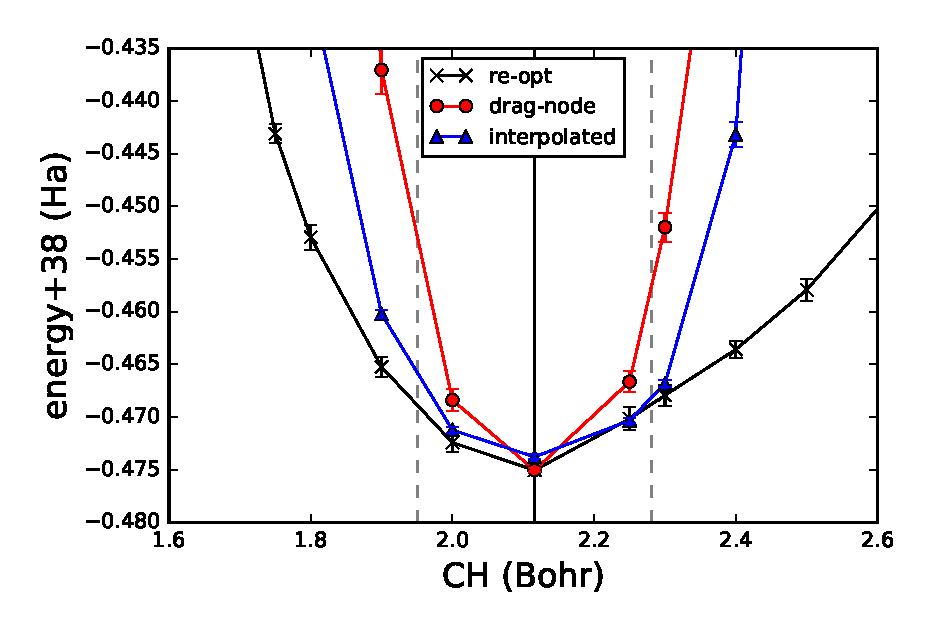
\includegraphics[width=0.8\textwidth]{ch-cold}
\caption{Clamped-ion VMC total energy as a function of C-H separation using a hierarchy of wave functions. The dashed lines mark the FWHM of the distribution of C-H separation.  Within the region marked by the dashed lines it can be seen that the interpolated wave function results are a closer match to the reference 're-opt' energies than the dragged-node energies. \label{fig:ch-cold}}
\end{figure}

%In our previous study, wave functions of the form in Eq. (2) were used to
%simulate several different molecular systems (6).
To determine the nonadiabatic contribution for each system,
we partition the energy into different components,
which includes the clamped-ion energies, the zero point energy (ZPE) and the
diagonal Born-Oppenheimer correction (DBOC). Everything that remained we
consider to be the nonadiabatic energy. Using standard quantum chemistry tools
all of the above terms can be calculated or approximated to high accuracy with
the exception of the nonadiabatic energy. As a result the nonadiabatic energy is
a quantity that has not been theoretically calculated for many systems. We see from Fig.~\ref{fig:dia-nad-ad} that the nonadiabatic energy was less than 0.1 mHa for most of the
systems considered. There are two exceptions, where the nonadiabatic energy
was larger, for the cases of BH and CH molecules.
Our new results for CH with the improved wave functions can be seen in Table~\ref{tab:nad-ch-energy}. Due to the variational property of FN-DMC, it is evident that these energies
are improved over the previous best results for the CH molecule, which is not
unexpected given the differences between the interpolated wave function and the
dragged-node wave function as seen in Figure~\ref{fig:ch-cold}. Our previous results showed a
nonadiabatic energy of 1.9 mHa, whereas our new results show a nonadiabatic energy of
0.9 mHa, which can be seen for the largest determinant expansion in Table~\ref{tab:nad-ch-energy}. This
is consistent with our previous results, mainly that the CH molecule is somewhat
nonadiabatic, even though our new estimate of the nonadiabatic energy is smaller.
For a system with a moderate amount of nonadiabatic energy, more effort is needed
in generating accurate wave functions. Improving the wave functions beyond the
dragged-node approximation will lower the estimate of the nonadiabatic energy,
but it is likely to remain somewhat large if the improvements of the wave function
correspond to degrees of freedom beyond the Born-Oppenehimer approximation.
This is what we see for CH, as the nonadiabatic energy is still relatively large in
comparison to other systems. We note that this is still not a definitive estimate of
the nonadiabatic energy, but it is likely the best estimate ever calculated for this
system.

\begin{table}[h]
\centering
\caption{DMC energy and variance with static ions, dynamic ions with dragged-node (``drag'') and dynamic ions with determinant coefficient interpolation (``interp.'').\label{tab:nad-ch-energy}}
\begin{tabular}{llll}
\hline\hline
$N_{\text{det}}$ & Energy (Ha) & Variance (Ha$^2$) & method \\
\hline
35   & -38.4709(1) &  0.3130(5) &    static \\
35   & -38.4622(2) &  0.3169(3) &   drag \\
35   & -38.4621(2) &  0.3173(3) &  interp. \\
723  & -38.4770(1)&  0.2489(3) &    static \\
723  & -38.4667(1) &  0.334(2)~  &   drag \\
723  & -38.4679(1) &  0.2713(7) &  interp. \\
4739 & -38.4781(1) &  0.2300(4) &    static \\
4739 & -38.4676(1) &  0.334(5)~  &   drag \\
4739 & -38.4687(2) &  0.267(7)~  &  interp. \\
\hline\hline
\end{tabular}
\end{table}

We also noticed interesting behavior that results from improving the quality
of the electron nodes. We performed clamped-ion (static) and fully nonadiabatic
(dynamic) calculations using different truncations levels for the determinant
expansion. The FN-DMC energy and variance for the various calculations are
shown in Table~\ref{tab:nad-ch-energy}. As we include more determinants in our wave function,
both the energy and variance of the static calculation decrease. However, the
same does not happen for the variance of the dragged-node approximation, in
which we see the surprising result that the variance increases. This suggests
that the clamped-ion wave functions are being improved to a larger extent than
the dragged-node wave functions with increasing determinant number. It is also
interesting to note that for the wave functions with the smallest determinant
expansion ($N_{det}$ = 35), the variance is almost the same between the clamped-ion
and dragged-node wave functions.
The energy and variance with determinant coefficient interpolation is
generally improved from our previous wave function with the dragged-node
approximation. A comparison between the dynamic runs with and without
interpolation also shows that coefficient interpolation becomes more important
for larger determinant expansions. In particular, the variance improves with
increasing determinant number, showing similar behavior to that of the static
wave function.

\begin{figure}[h]
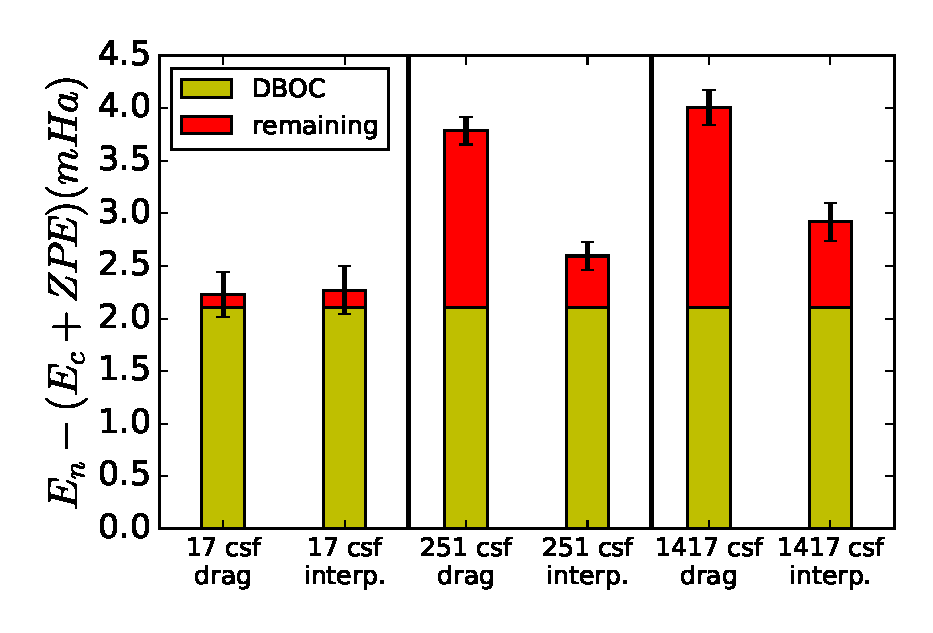
\includegraphics[width=0.8\textwidth]{ch-only}
\caption{Nonadiabatic energy of CH with and without determinant coefficient interpolation.  The wave function ``interp'' denotes that the determinant coefficients depend on C-H separation through linear interpolation. For the largest two determinant expansions a more significant contribution from nonadiabatic effects is observed than the smallest determinant expansion. \label{fig:ch-interp} }
\end{figure}

In Figure~\ref{fig:ch-interp}, we show the various contributions to the difference between
the static and dynamic ground-state energies. Due to the difference in energy
scales for the quantities of interest, we only plot the diagonal Born-Oppenheimer
energy and the nonadiabatic energy. To calculate the nonadiabatic energy we
take the estimated zero-point energy for CH to be 6.438 mHa~\cite{Feller_Corrections}. The diagonal
Born-Oppenheimer correction is estimated to be 2.11 mHa. Our best result is
given by the 4739 determinant interpolated wave function in Figure~\ref{fig:nonbo-ch-star}. There is an apparent increase in the nonadiabatic energy of the CH molecule that results
from using the dragged-node approximation. The improvement seen by using the
interpolated wave function instead of the dragged-node approximation is 1 mHa
for the CH molecule; a relatively large change in the energy.
That the dragged-node approximation produced such a large error
for the CH molecule suggests at the very least that the nodal structure of its wave
function has more complex dependence on the ion configuration than the rest of
the molecules under consideration.

\begin{figure}[h]
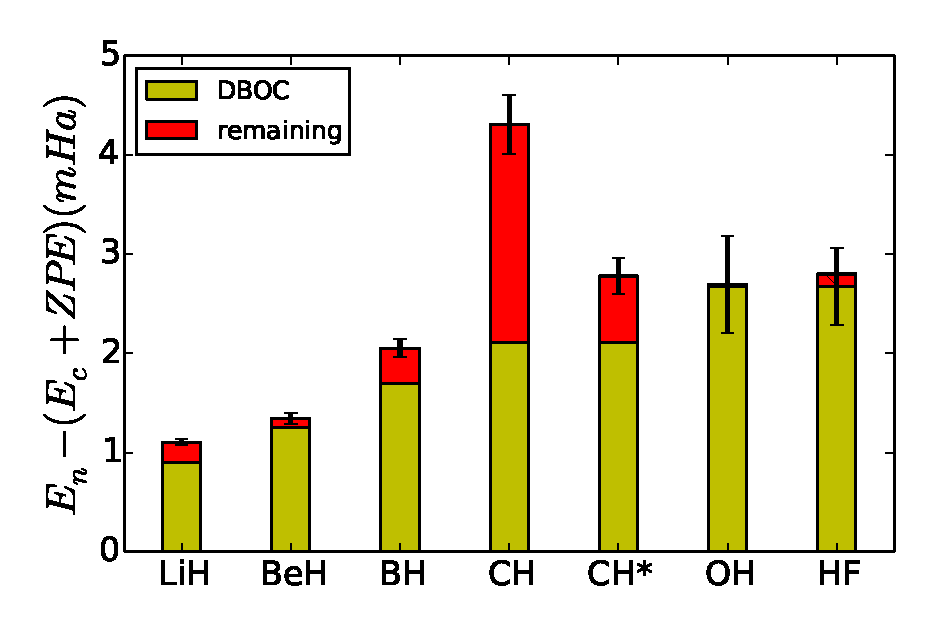
\includegraphics[width=0.8\textwidth]{4738}
\caption{Nonadiabatic energy of diatomic molecules. The best (4739
determinant) result for CH with determinant coefficient interpolation is shown
with *. Note that for all the molcules except for BH and CH the nonadiabatic
energies are roughly 0.1 mHa or smaller.}
\label{fig:nonbo-ch-star}
\end{figure}

Figure~\ref{fig:ch-interp} also reveals that the nonadiabatic energy is only observed with the
large determinant expansions. There are several possible explanations for this. It
is possible we are optimizing the static wave function significantly better than the
electron-ion wave function. There is some indication of this from the variance
of the dragged-node approximation, but this is less evident for the interpolated
wave function. Another possible explanation is that only when the wave function
is highly optimized do significant changes arise in the wave function amplitudes
with regard to ion positions. A related effect is that large fluctuations of the ion
distance can be suppressed if the wave function and the related nodal surface is
not well optimized at large ion distances. Such effects can be mitigated
with the interpolated wave function approach, and are likely to be suppressed with
increasing the number of determinants for the electronic part of the wave function,
even for the dragged-node wave function. In Fig.~\ref{fig:nonbo-ch-star}, we compare our improved results
for CH with the nonadiabatic contributions from previous work. It is evident
that the CH nonadiabatic energy is still larger than all the other molecular
systems.

\section{Conclusion}
We calculated the ground-state energies of first-row atoms and their corresponding ions and hydrides with and without the Born-Oppenheimer approximation. In addition, we examined the amount of nonadiabatic contribution to the ground-state energies of all systems studied and determined the amount to be up to a few mHa. In the case of CH, the nonadiabatic effects beyond the DBOC appeared to be unusually large, although we found that a large part of this discrepancy was due to the fixed-node error.
To this end, we improved the electron-ion wave functions for diatomic systems by interpolating determinant coefficients as a function of ion separation.
Even with the improved wave function, there is still a slightly larger contribution from nonadiabatic effects in CH.

We found the ionization energies of the atoms to be independent of the Born-Oppenheimer approximation, consistent with a previous high-level quantum chemistry study.~\cite{Klopper_IP} In contrast, the atomization energies of the hydrides showed effects of nonadiabaticity, although they were generally much less than 1 mHa. This work obtained the first nonadiabatic QMC benchmark data for non-relativistic ground-state energies and obtained the lowest variational result for BH and the only results for CH, OH and HF, to the best of our knowledge.

%In comparing to accurate benchmark results obtained with other methods, we have demonstrated the validity of our wave function ansatz, namely it does produce a high-quality electron-ion wave function. This technique also has the potential to solve interesting larger-scale problems due to its ease of implementation, as well as the polynomial scaling in computational time with respect to the number of electrons.

%\bibliography{nonbo-ref}
%\chapter{Dynamic-ion DMC Study of Solid Hydrogen at Megabar Pressures}
\label{chap:hsolid}
\section{Introduction}

% why is hydrogen under pressure interesting?
The properties and phase transitions of hydrogen under megabar pressures are important in diverse fields of study. For astronomy, models of the interior of giant gas planets such as Jupiter and Saturn depend critically on the nature of the molecular liquid to atomic liquid transition (LLT), namely whether it is first-order or continuous~\cite{Hubbard2016,Wahl2017}. For condensed matter, metallic hydrogen holds promise for a room temperature conventional superconductor~\cite{McMahon2011,McMahon2012}. For computational physics, hydrogen remains an important benchmark for both electronic structure~\cite{Motta2017} and ion dynamics methods. With no need for a pseudopotential, simulations of hydrogen avoid a significant source of bias. However, the low mass of the nuclei necessitates quantum treatment of the lattice degree of freedom, often beyond the harmonic approximation, in accurate simulations.

\begin{figure}[h]
\centering
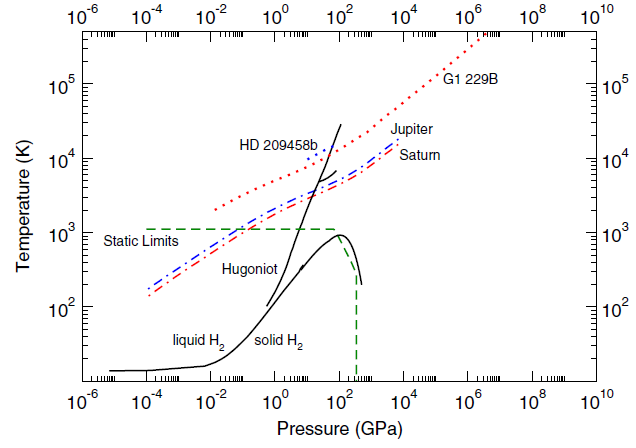
\includegraphics[width=0.6\linewidth]{mcmahon-phases}
\caption{Partial phase diagram of hydrogen on log-log scale~\cite{McMahon2012rmp}.}
\end{figure}

% what controversies are there in experiment?
Established experimental results on high-pressure hydrogen are limited. At room temperature and below, diamond anvil cell (DAC) is the dominant apparatus to achieve such high pressures. Small size of the cell and fragility of the sample limit experimental probes to low-power optics such as infrared and Raman spectroscopy\cite{RangaI.F.2017}. Hydrogen is a weak scatterer of X-Rays~\cite{Zha2014}, thus excluding this excellent tool for structural determination in most experiments. Only recently has X-ray analysis been performed up to 254 GPa~\cite{Akahama2010,Ji2019}.
At high temperatures, shock wave compression is the main method to achieve megabar pressures. Due to the transient nature of theses experiments, acquiring and analyzing shock-wave data is challenging. Most notably, one cannot directly measure temperature, which may cause misinterpretation of raw data~\cite{Celliers2018,Knudson2004,Knudson2017}.
Given the experimental difficulties, predictive simulations are highly desirable as they can inform and verify experiments~\cite{Pierleoni2016b}.

% what controversies are there in calculations?
Simulation of high-pressure hydrogen is also challenging. Without experimental structural information from X-ray, many theoretical calculations have been performed on structures found in density functional theory (DFT) random structure searches~\cite{Pickard2007}. Constrained by computational cost, these searches are limited to classical protons, causing the methods to miss, for example, saddle-point structures that can be stabilized by nuclear quantum effect~\cite{Monserrat2016}.
%Most theoretical studies of high-pressure hydrogen suffer a similar dilemma between accuracy and practicality.
%On the one hand,
Predictive simulations of hydrogen require accurate methods both in the description of the electronic ground-state Born-Oppenheimer (BO) potential energy surface (PES) and in the inclusion of nuclear quantum effect beyond the quasi-harmonic approximation.
%On the other hand, to explore such large pressure and temperature ranges using first-principle methods is not only time consuming, but also prone to other limitations such as inadequate treatment of finite-size effect, nuclear quantum effect, and simulation timescale. Further, some experimentally measurable properties, such as emission, absorption, infrared, and Raman spectra, heat conductivity, and diffusion constants are difficult to calculate in the most accurate electronic methods, e.g., DMC.
The popular Perdew-Burke-Ernzerhof (PBE) density functional in DFT erroneously predicts some molecular structures to be metallic~\cite{Drummond2015}. However, its use in conjunction with Classical molecular dynamics (MD) results in reasonable transition pressure for the LLT at certain temperatures due to error cancellation~\cite{Morales2013a}.
This and other fortuitous cancellations of error has led many to believe that the PBE functional provides a good description of solid hydrogen and caused much confusion in the community. PBE predicts a conductive molecular structure above 200 GPa, a molecular-to-atomic transition around 300 GPa~\cite{McMinis2015}, and low-temperature superconducting liquid. All these predictions contradict experimental evidence. Systematic benchmark of the PES from various DFT functionals against QMC found the vdW-DF1 functional to be the most accurate for molecular hydrogen~\cite{Clay2016}. However, this functional has yet to gain widespread adoption due to its higher computational cost and lower popularity compared to PBE.

In this chapter, I will focus on the solid phases of hydrogen. Sec.~\ref{sec:hsolid-expt} summarizes experimental observations, Sec.~\ref{sec:hsolid-calcs} summarizes relevant computational studies,
Sec.~\ref{sec:hsolid-methods} details the approach taken in this study,
and Sec.~\ref{sec:hsolid-results} presents the computational results.

\subsection{Experiments}
\label{sec:hsolid-expt}

As element number one with the simplest atomic structure, hydrogen has surprisingly complex phases at megabar pressures.
Further complicating matters, the phase diagram depends on the isotopes, e.g., hydrogen H, deuterium D, and spin isomers of molecular hydrogen.
The proton spins anti-align to form a singlet para-hydrogen (p-H$_2$), whereas they align to form a triplet in ortho-hydrogen (o-H$_2$).
To clarify the narrative, I will first introduce the well-established phases in pure samples, then discuss changes due to isotopic and ortho-para conversion.

For pure p-H$_2$ at low temperature (5$\sim$10 K), three solid phases are well-established. The low-pressure phase (LP) below 100 GPa is a molecular crystal having spherically symmetric H$_2$ molecules on hcp lattice sites. Above 110 GPa, hydrogen enters a broken-symmetry phase (BSP), where anisotropic intermolecular interactions favor the $J=2$ $v=1$ vibrational state of the H$_2$ molecules rather than the spherically symmetric $J=0$ $v=1$ state~\cite{Lorenzana1990}. Above 160 GPa, after crossing a first-order transition, one finds an orientationally-ordered phase known as the A phase (H-A)~\cite{Lorenzana1989}.

The transition from LP to BSP phase is sensitive to isotope and nuclear spin. o-D$_2$, HD, and p-H$_2$ enters the BSP at 28 GPa~\cite{Silvera1981}, 70 GPa~\cite{Chijioke2006}, and 110 GPA~\cite{Lorenzana1990}, respectively. o-H$_2$ and p-D$_2$ have a hcp to fcc transition at ambient pressure. In contrast, the transition to the A phase is fairly robust across isotope and spin isomer variants. HD, o-D$_2$, and p-H$_2$ all enter the A phase between 150 and 160 GPa~\cite{Hemley1988,Lorenzana1989,Cui1994,Chijioke2006}. The phase lines for o-D$_2$ and HD are shown in Fig.~\ref{fig:hsolid-phases123}. The p-H$_2$ LP-BSP phase line near 100 GPa is not shown. The size and shape of the BSP is the only difference between the phase diagrams of p-H$_2$, o-D$_2$, and HD.

\begin{figure}[h]
\centering
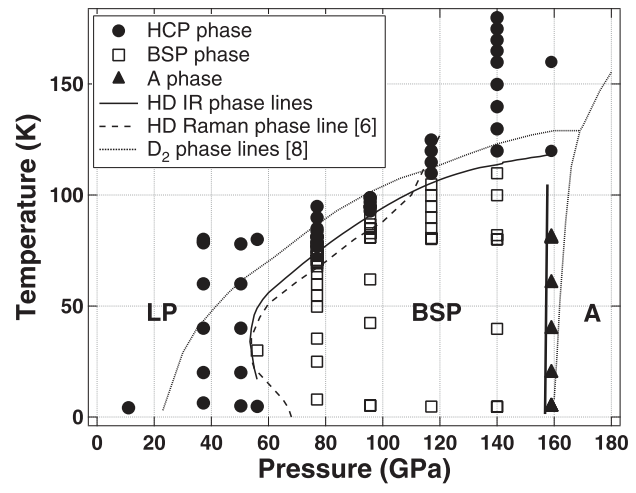
\includegraphics[width=0.6\linewidth]{phases123}
\caption{Phase diagram of o-D$_2$ and HD below 200 K and 200 GPa~\cite{Chijioke2006}.}
\label{fig:hsolid-phases123}
\end{figure}

Transitions to these orientationally ordered phases are detected by changes in Raman and IR spectra. As shown in Fig.~\ref{fig:hsolid-p-h2-bsp}, during the LP to BSP transition, one can observe clear broadening and weakening of the low-frequency roton bands around 350 cm$^{-1}$ and an associated small (15 cm$^{-1}$) discontinuity in the position of the vibron peak, which is about 4150 cm$^{-1}$ near the transition pressure 110 GPa~\cite{Lorenzana1990}. Upon further increase of pressure past 160 GPa, a much larger discontinuity of the Raman vibron (100 cm$^{-1}$) signals the onset of the A phase~\cite{Hemley1988,Lorenzana1989}. A direct transition from H-A back to the LP phase can be achieved by raising temperature. Across this transition, the intensities of the libron bands decrease discontinuously~\cite{Lorenzana1990}.

\begin{figure}[h]
\centering
\begin{minipage}{0.38\columnwidth}
\centering
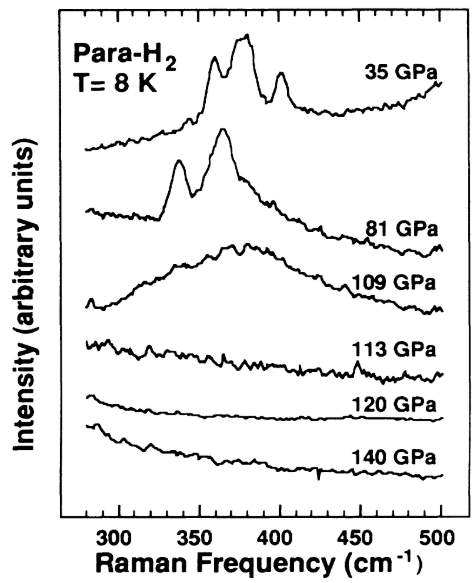
\includegraphics[width=\columnwidth]{p-h2-bsp-rotons}
(a) rotons
\end{minipage}
\begin{minipage}{0.58\columnwidth}
\centering
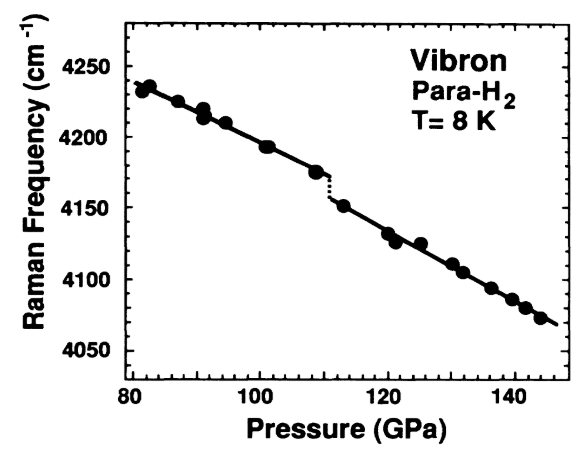
\includegraphics[width=\columnwidth]{p-h2-bsp-vibron}
(b) vibron
\end{minipage}
\caption{Roton and vibron changes in p-H$_2$ across the BSP transition~\cite{Lorenzana1990}.}
\label{fig:hsolid-p-h2-bsp}
\end{figure}

The optical signatures for the LP to BSP transition in o-D$_2$ are qualitatively similar to those in p-H$_2$. The vibron decreases discontinuously by 3 cm$^{-1}$ rather than 15 cm$^{-1}$, while the roton bands broaden and weaken near the transition pressure of 28 GPa rather than 110 GPa~\cite{Silvera1981}. Further confirmation of these two phase transitions were later obtained from IR absorption spectra~\cite{Cui1994}. Three absorption peaks appear around 3150 cm$^{-1}$ upon entering the BSP phase and are replaced by a single broad peak at the same frequency range when the A phase is reached. The same signatures were used to identify the BSP and A phases of HD at 70 and 160 GPa, respectively~\cite{Chijioke2006}.
In the A phase, the rather broad and pressure-independent roton band weakens, disappears, and is replaced by a few sharp and strongly pressure-dependent peaks in the frequency range 100$\sim$700 cm$^{-1}$~\cite{Goncharov1998}.
These new modes are considered to be lattice libration modes due to their pressure dependence.

%As pressure increases, anisotropic intermolecular interactions mix the free roton states until the ground state distorts and molecules become orientationally ordered to lower potential energy. This broken-symmetry phase (BSP) or phase II, stable under 140 K, is considered a quantum phase based on observed strong isotope shift of the transition pressure. o-D$_2$ reaches the BSP phase at as low as 28 GPa at 1.1 K~\cite{Silvera1981}.

Phases with mixed ortho-para concentrations of H$_2$ are labeled I, II, and III~\cite{Dias2016,Dias2019}, which correspond to the LP, BSP, and H-A phases of pure p-H$_2$, respectively.
As shown in Fig.~\ref{fig:hsolid-phases}, at 300 K and above 220 GPa, we enter yet another solid phase IV, characterized by a splitting of the vibron peak~\cite{Zha2013}.
Both theory and experiment suggest that phase IV consists of alternating layers having rather different in-plane structures, possibly two types of molecules.
Below 100 K and above 350 GPa, molecular hydrogen becomes semi-metallic, possibly due to the closure of an indirect band gap~\cite{Eremets2019}.
Then, above 425 GPa, all IR radiation is absorbed indicating a closure of the direct band gap~\cite{Loubeyre2020}.
Finally, at sufficiently high pressures, the hydrogen molecules will dissociate to form an atomic solid, reportedly at 495 GPa~\cite{Silvera2017}, although consensus has yet to be reached.

\begin{figure}[h]
\centering
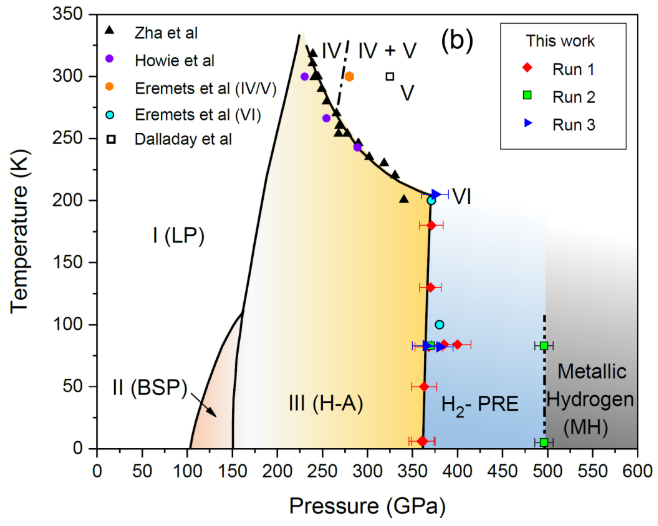
\includegraphics[width=0.6\linewidth]{hsolid-phases}
\caption{Tentative phase diagram of solid hydrogen below 400 K~\cite{Dias2019}.}
\label{fig:hsolid-phases}
\end{figure}

While the phase boundaries of solid hydrogen are reasonably well-established below 400 K and 400 GPa by diamond-anvil cell (DAC) experiments, characterizations of the solid structures are limited. Due to the small scattering cross section and small sample size in DAC experiments, only a handful of X-ray~\cite{Hazen1987,MAO1988,Loubeyre1996,Kawamura2002,Goncharenko2005a,Akahama2010,Ji2019} and only one neutron~\cite{Goncharenko2005a} scattering experiments have been published over the past 40 years. Most of our understanding of solid hydrogen is built upon IR and Raman spectra, which provide partial information on the microscopic details of the solid structures. This lack of definitive structural information poses significant difficulty for both theoretical and experimental understanding of solid hydrogen. Experimentally, this has lead to the misidentification of a triple point as a critical point~\cite{Lorenzana1990,Cui1994}, subtlety in the detection of a new phase~\cite{Eremets2009,Howie2012}, among many debates over interpretation of optical data.

\subsection{Calculations}
\label{sec:hsolid-calcs}

Early computational studies of solid hydrogen rely on assumed crystal structures from known high-pressure phases of other materials or simple symmetry and energetic arguments. Even before the observation of the oriented A phase of solid hydrogen~\cite{Hemley1988}, S. Raynor~\cite{Raynor1987} used Hartree-Fock and perturbation theory to show that the molecular hexagonal closed packed structure with H$_2$ molecules aligned along the c-axis (mhcp-c) is more energetically favorable than previous considered cubic structures.
While a promising candidate for phase III~\cite{Barbee1989}, the mhcp-c structure has an early band overlap, rendering it metallic below 150 GPa, resists compression along the c-axis, and has no IR-active vibron~\cite{Kaxiras1991,Kaxiras1992}, all in contradiction with experimental evidence.
Thus, E. Kaxiras \textit{et al.}~\cite{Kaxiras1991} explored different orientations of H$_2$ molecules in the 2-atom hcp unit cell and found a more energetically favorable insulating structure with molecules oriented $\sim$60$^{\circ}$ from the c-axis.
This static-lattice LDA study was later validated by a dynamic-lattice QMC calculation~\cite{Natoli1995}, and the structure named mhcp-o.
In addition to the hcp structures, H. Nagara and T. Nakamura~\cite{Nagara1992} proposed various rutile structures by minimizing the static-lattice electric quadrupole-quadrupole (EQQ) interactions, while B. Edwards, N. W. Ashcroft, and T. Lenosky~\cite{Edwards1996} proposed an orthorhombic layered structure of Cmca symmetry, which turned out to be metallic at pressures relevant to phase III~\cite{Johnson2000}.
This Cmca crystal structure also appeared spontaneously in path integral simulation~\cite{Cui2002}.
These theoretical calculations drove much debate about the fate of phase III at pressures over 300 GPa. Does it become a metallic molecular solid or does it dissociate into an atomic solid without the band gap closing?

In 2007, the advent of random structure searching produced new candidate crystal structures that have lower enthalpy than previous proposals~\cite{Pickard2007}. The insulating layered structure having C2/c symmetry became the main candidates for phase III.
Three diffusion Monte Carlo studies followed to characterize the candidate structures by Azadi \textit{et al.}~\cite{Azadi2014}, McMinis \textit{et al.}~\cite{McMinis2015}, and Drummond \textit{et al.}~\cite{Drummond2015}.
Azadi \textit{et al.} used PBE-optimized geometries and included anharmonic phonon zero-point energy, leading to a molecular dissociation at 374 GPa, from Cmca-12 to I4$_1$/amd.
In contrast, McMinis \textit{et al.} used vdW-DF-optimized geometries and harmonic phonon zero-point energy to predict a dissociation pressure of 447(3) GPa.
In hind sight, the prediction by McMinis \textit{et al.} is in better agreement with subsequent experiments.

On the low pressure side, a new hexagonal candidate structure for phase III was proposed by Monserrat \textit{et al.}~\cite{Monserrat2016} in 2016, then calculated to be more stable than C2/c below 210 GPa~\cite{Azadi2019}.
Bandgap of the C2/c structure shows closure around 460 GPa, when extrapolated from  was IR measurements up to 420 GPa~\cite{Loubeyre2020}, with the most recent DMC calculation in agreement~\cite{Gorelov2019}. This new calculation is at variance with the previous prediction by Azadi \textit{et al.}~\cite{Azadi2019}, presumably due to different treatments of finite-size effects.
Finally, a recent coupled cluster calculation of the molecular candidate structures show good agreement with DMC results~\cite{Liao2019} at the static lattice level, although lattice zero-point energy has yet to be included.

In this chapter, we examine the most promising candidate structures using dynamic-lattice DMC.
This method treats the electrons and ions on the same footing while harnessing the accuracy of DMC.
Lattice vibrations are included beyond the harmonic approximation and nonadiabatic effects can be captured.
The goal is to provide the most accurate properties of the solid hydrogen phases.
%The goal is to combine and improve upon the best methods in all previous QMC studies and provide the most accurate properties of the solid hydrogen phases.

%\subsection{The melting transition and critical point}
%
%The melting temperature of solid hydrogen is typically determined in one of three ways: 1. visual observation of motion due to sample, contaminant, or laser speckle~\cite{Gregoryanz2003}, 2. discontinuous change in the Raman spectrum, e.g. vibron frequency jump, disappearance of librons~\cite{Gregoryanz2003,Subramanian2011,Zha2017}, 3. plateau temperature during laser heating~\cite{Deemyad2008}, and 4. rapid change in interferences pattern~\cite{Eremets2009}.
%As sample size decreases with pressure, visual detection of melting becomes more difficult. Further, the refractive indexes of hydrogen and diamond approach each other around 140 GPa, defeating detection by interference pattern~\cite{Zha2017}.
%The vibron discontinuity caused by melting reduces from $\sim$ 3 cm$^{-1}$ at 10 GPa to $\sim$ 1 cm$^{-1}$ at 45 GPa~\cite{Gregoryanz2003}, making melting detection more difficult at higher pressures.
%Finally, disappearance of librons alone cannot be taken as proof of melting, because it could be due to loss of sample.
%Due to these difficulties, the precise melting temperatures above 100 GPa are debate. Although, there is broad consensus that the melting line increases from 200 K at ambient pressure to $\sim$ 1000 K at 90 GPa, then decreases with increasing pressure.
%
%Melting of $H_2$ solid around 150 GPa is particularly interesting. Shock wave compression data indicate a molecular liquid to atomic liquid transition $\sim$ 1000 K at 150 GPa. Thus, $H_2$ molecules should dissociate almost immediately after the solid melts. Eremets and Trojan observed a shark drop in measured resistivity as the $H_2$ solid melts at 146 GPa~\cite{Eremets2009}. This observation is consistent with the current liquid-liquid transition (LLT) line.
%%\section{Geometry Optimization}
% hsolid/11-refine-struct/a-ecut
The molecular structures are optimized in DFT using the vdW-DF functional. We use quantum ESPRESSO v5.3.0 to perform variable-cell geometry optimization at constant pressure. The atomic positions in the optimized unit cell are re-optimized at constant-volume. We use a Troullier-Martins pseudopotential with a core cutoff radius of $r_c=0.5$. The plane-wave cutoff energy is set to 160 Ry. Brillouin zone integration is performed using a shifted Monkhorst-Pack grid with $24^3$, $16^3$, $12^3$ points for the Cmca-4, Cmca-12, and C2/c-24 unit cells, respectively. %The effective number of atoms are 55296, 49152, and 41472, respectively.
Pressure is converged to 0.1 kbar (0.01 GPa). % Forces are converged to

The atomic structure is optimized in DMC. At each density, the $c/a$ parameter determines the I4$_1$/amd-4 ($c/a>1$) crystal structure. To optimize the $c/a$ parameter, we performed 5 DMC calculations at each density. These calculations form a grid in the lattice a-c parameter space as shown in Fig.~\ref{fig:i4-rs-ca}. Please see QMC section for details of the DMC calculations.
\begin{figure}[h]
% 2018-02-01_ani-press
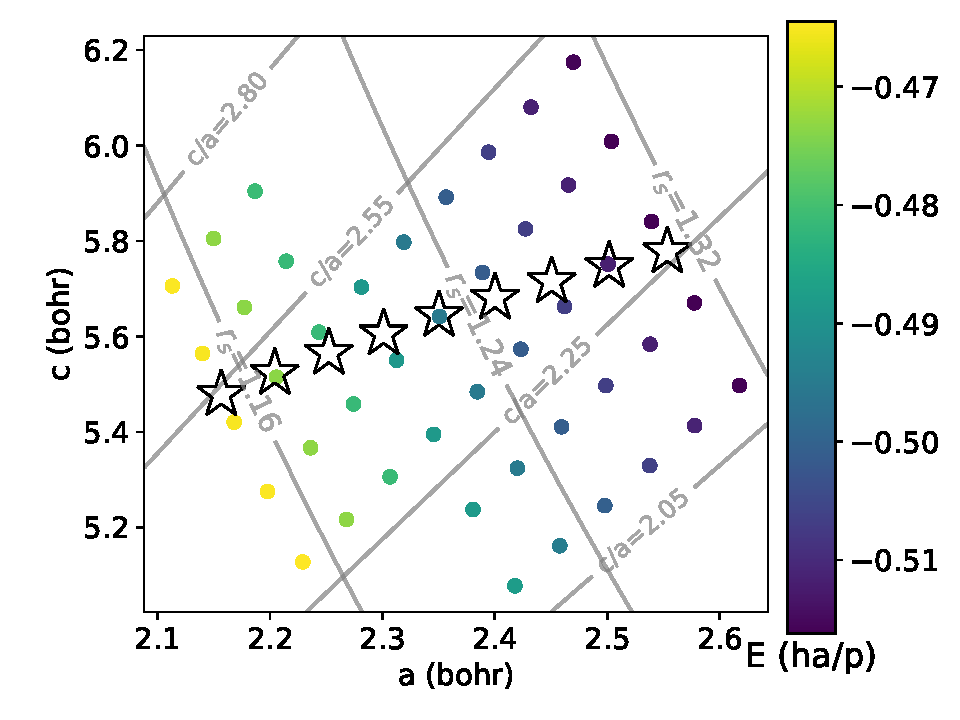
\includegraphics[width=0.8\columnwidth]{70_i4_ca_grid}
\caption{DMC calculations performed to optimize the atomic hydrogen solid structure. Each dot is a structure defined by the lattice parameters a and c. The color of each dot indicates the DMC energy. The gray contour lines mark structures with constant density or c/a ratio. Energy variation is dominated by density change. Energy variation in the c/a direction at fixed density is roughly quadratic around its minimum (black star). The black stars are the optimized geometries.\label{fig:i4-rs-ca}}.
\end{figure}

\section{Relative Enthalpy of Optimized Structures in DFT}
The enthalpies of the optimized crystal structures are calculated in DFT using the vdW-DF functional. As shown in Fig.~\ref{fig:dft-opt-geo},our relative enthalpies agree within 1.5 meV/p with those from McMinis et. al.. Our relative enthalpies for Cmca-12 agree within 1 mha/p with both those from Drummond et. al. and those from McMinis et. al.. Our relative enthalpy for Cmca-4 is higher than that of Drummond by 3.4 mha/p at 400 GPa. % Q/ Is the 3.4 mha/p difference due to structure or functional?
\begin{figure}[h]
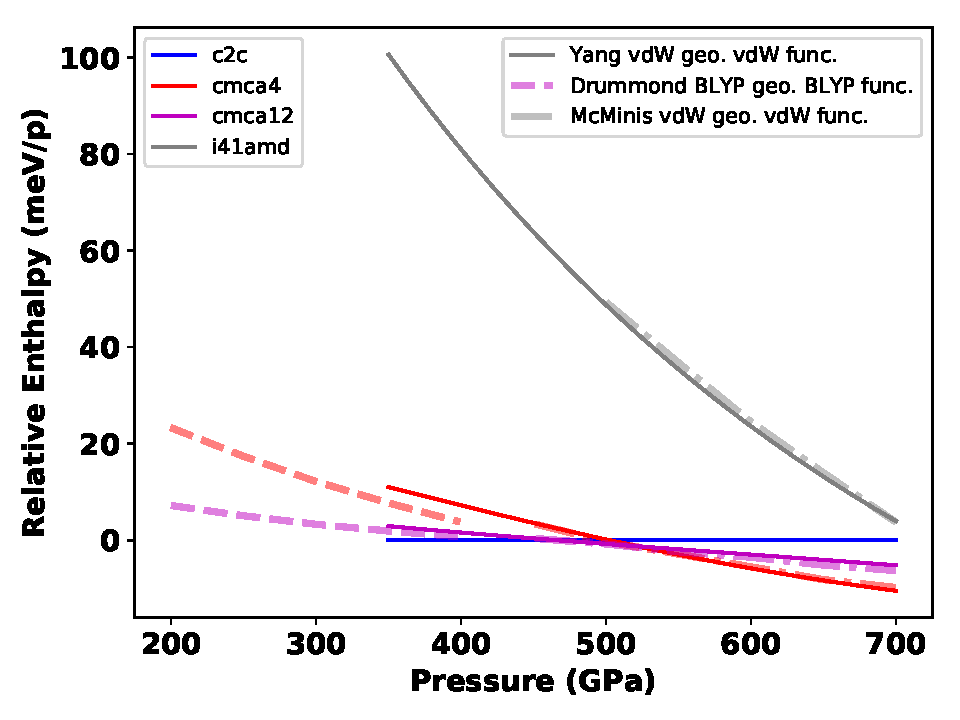
\includegraphics[width=0.8\columnwidth]{010a_dh-vs-p}
\caption{DFT(vdW-DF) enthalpy of optimized structures relative to C2/c-24. Thin solid lines are enthalpies of the Cmca-4, Cmca-12 and I4$_1$/amd using our optimized structures. Dashed lines are DFT(BLYP) enthalpies of Cmca-4 and Cmca-12 from Drummond et. al.. Dash-dot lines are DFT(vdW) enthalpies from McMinis et. al..\label{fig:dft-opt-geo}}
\end{figure}

\subsection{Wavefunction}

All QMC calculations are performed using the QMCPACK code. We use Slater-Jastrow-Backflow (SJB) wavefunction. The orbitals in the Slater determinant are cusp-corrected DFT orbitals. The vdw-DF functional is used to generate orbitals for the molecular structures, whereas the PBE functional is used for the atomic structure. The orbital generating DFT runs have different settings compared to the geometry optimization runs.

To generate the orbitals, we perform DFT directly in the supercell. All calculations use the bare Coulomb interaction and a plane wave cutoff of 50 Ry. First, we run a self-consistent calculation to converge the charge density on a shifted $8^3$ Monkhorst-Pack grid. Second, we run a non-self-consistent calculation on an unshifted Monkhorst-Pack grid to generate the orbitals needed by all twists. $4^3$ twists are used for the molecular phase, while $6^3$ twists are used for the atomic phase. Finally, we divide each orbital by an electron-ion Jastrow wavefunction to remove the electron-ion cusp from the orbital. This electron-ion Jastrow wavefunction is constructed using Fourier components commensurate with the simulation cell (i.e. on the reciprocal lattice vectors of the simulation cell $\bs{G}_s$)
\begin{align}
J_{ei}(\bs{r}_j; \bs{R}) \propto& \exp\left\{ \text{iFFT}\left[ 
U_{\bs{k}}^{ep}  \left(\sum\limits_{J=1}^{N_p} \frac{e^{-i\bs{k}\cdot\bs{R}_J}}{N_p}  \right)
\right] \right\} \nonumber\\
\propto& \exp\left\{ 
\sum\limits_{\bs{k}\neq\bs{0}}^{\bs{k}\in\bs{G}_s} e^{i\bs{k}\cdot\bs{r}_j}~
U_{\bs{k}}^{ep} 
\left(\sum\limits_{J=1}^{N_p} \frac{e^{-i\bs{k}\cdot\bs{R}_J}}{N_p}  \right)
\right\},\label{eq:rpa-ep-jas}
\end{align}
where $\bs{r}_j$ is any single electron coordinate. $\bs{R}$ contains all ionic coordinates. $N_p$ is the number of protons. iFFT stands for ``inverse fast Fourier transform''. The Jastrow potential $U_{\bs{k}}^{ep}$ in eq.~(\ref{eq:rpa-ep-jas}) is chosen to be the RPA form written by Ceperley and Alder
\begin{align}
2U^{ep}_k = -a_k(1+a_k)^{-1/2},
\end{align}
where $a_k=\frac{12}{r_s^3k^4}$ in Hartree atomic units. $r_s$ is the Wigner-Seitz radius.

When a single-particle orbital is divided by eq.~(\ref{eq:rpa-ep-jas}), the electron-ion cusp is removed from the orbital. We re-introduce the electron-ion cusp in the Jastrow part of the trial wavefunction. 

There are 48 optimizable parameters in our wavefunction. We use short-range B-spline Jastrow pair potentials which are smoothly cut off at $R_{WS}$ (the image radius). There are three Jastrow potentials (uu, ud, ep) between up and up electrons, up and down electrons, electron and proton. We use short-range B-spline back flow transformation functions which are smoothly cut off $R_{WS}$. There are three backflow correlation functions (uu, ud, ep) similar to the Jastrow setup. Each B-spline has 8 optimizable knots.
\begin{comment}
\subsection{QMC Data}

At each density, we perform one VMC and two DMC calculations. Each QMC calculation is labeled by a series index. The VMC calculation is series 0. The first DMC calculation with a relatively large time step is series 1. The second DMC calculation with a relatively small time step is series 2. We post-process the raw results (series 0 - 2) to produce series 3 and 4. We linearly extrapolate the DMC results (series 1, 2) to zero time step and label the results series 3. We linearly extrapolate the VMC and the t=0 DMC results (series 0, 3) to obtain pure-estimator kinetic and potential energies and label them series 4.

Twist-average QMC energies are displayed in the following table. The dUlr column contains the many-body finite size correction which will be described in the next section.

\begin{table}[h]
\small
\begin{tabular}{llrrrllll}
\toprule
         &   &  timestep &  natom &      dUlr & LocalEnergy\_pp &    Variance\_pp &     Kinetic\_pp &    Potential\_pp \\
rs & series &           &        &           &                &                &                &                 \\
\midrule
1.163891 & 0 &    0.0300 &     72 &  0.005586 &    -0.47572(1) &     0.01380(2) &      0.9819(1) &      -1.4576(1) \\
         & 1 &    0.0030 &     72 &  0.005417 &   -0.477138(9) &    0.013719(9) &     0.98177(9) &     -1.45890(8) \\
         & 2 &    0.0015 &     72 &  0.005404 &    -0.47712(1) &     0.01374(1) &      0.9822(1) &    -1.45933(10) \\
         & 3 &    0.0000 &     72 &  0.005391 &    -0.47711(2) &     0.01374(1) &      0.9827(2) &      -1.4598(2) \\
         & 4 &    0.0000 &     72 &  0.005213 &    -0.47711(2) &     0.01374(1) &      0.9834(2) &      -1.4598(2) \\
1.182675 & 0 &    0.0300 &     72 &  0.005455 &    -0.48354(1) &     0.01347(2) &      0.9581(1) &      -1.4416(1) \\
         & 1 &    0.0030 &     72 &  0.005269 &   -0.484951(9) &    0.013408(8) &     0.95828(9) &     -1.44323(9) \\
         & 2 &    0.0015 &     72 &  0.005287 &    -0.48496(1) &     0.01342(1) &      0.9585(1) &      -1.4434(1) \\
         & 3 &    0.0000 &     72 &  0.005305 &    -0.48496(2) &     0.01342(1) &      0.9587(2) &      -1.4436(2) \\
         & 4 &    0.0000 &     72 &  0.005170 &    -0.48496(2) &     0.01342(1) &      0.9592(2) &      -1.4436(2) \\
1.195717 & 0 &    0.0300 &     72 &  0.005373 &   -0.488647(6) &    0.012795(9) &     0.94365(7) &     -1.43230(7) \\
         & 1 &    0.0030 &     72 &  0.005188 &   -0.490019(9) &    0.012688(8) &     0.94357(9) &     -1.43361(9) \\
         & 2 &    0.0015 &     72 &  0.005183 &   -0.490017(9) &    0.012707(9) &     0.94391(9) &     -1.43394(9) \\
         & 3 &    0.0000 &     72 &  0.005178 &    -0.49002(2) &    0.012707(9) &      0.9443(2) &      -1.4343(2) \\
         & 4 &    0.0000 &     72 &  0.004997 &    -0.49002(2) &    0.012707(9) &      0.9449(2) &      -1.4343(2) \\
1.221845 & 0 &    0.0300 &     72 &  0.005135 &   -0.497976(6) &    0.012288(9) &     0.91589(7) &     -1.41386(7) \\
         & 1 &    0.0030 &     72 &  0.004973 &   -0.499383(8) &    0.012232(9) &     0.91531(9) &     -1.41469(9) \\
         & 2 &    0.0015 &     72 &  0.004998 &   -0.499352(8) &    0.012255(9) &     0.91567(9) &     -1.41501(9) \\
         & 3 &    0.0000 &     72 &  0.005023 &    -0.49932(2) &    0.012255(9) &      0.9160(2) &      -1.4153(2) \\
         & 4 &    0.0000 &     72 &  0.004922 &    -0.49932(2) &    0.012255(9) &      0.9162(2) &      -1.4153(2) \\
1.235307 & 0 &    0.0300 &     72 &  0.005067 &   -0.502414(6) &     0.01188(1) &     0.90195(6) &     -1.40436(7) \\
         & 1 &    0.0030 &     72 &  0.004900 &   -0.503809(8) &    0.011814(8) &     0.90131(9) &     -1.40508(9) \\
         & 2 &    0.0015 &     72 &  0.004908 &   -0.503783(9) &    0.011793(9) &     0.90181(9) &     -1.40559(9) \\
         & 3 &    0.0000 &     72 &  0.004915 &    -0.50376(2) &    0.011793(9) &      0.9023(2) &      -1.4061(2) \\
         & 4 &    0.0000 &     72 &  0.004776 &    -0.50376(2) &    0.011793(9) &      0.9027(2) &      -1.4061(2) \\
1.249707 & 0 &    0.0300 &     72 &  0.004887 &   -0.506825(6) &     0.01274(2) &     0.88739(7) &     -1.39422(7) \\
         & 1 &    0.0030 &     72 &  0.004748 &   -0.508268(9) &    0.012682(9) &      0.8869(1) &     -1.39525(9) \\
         & 2 &    0.0015 &     72 &  0.004765 &   -0.508273(9) &    0.012696(9) &     0.88747(9) &     -1.39574(9) \\
         & 3 &    0.0000 &     72 &  0.004783 &    -0.50828(2) &    0.012696(9) &      0.8880(2) &      -1.3962(2) \\
         & 4 &    0.0000 &     72 &  0.004690 &    -0.50828(2) &    0.012696(9) &      0.8886(2) &      -1.3962(2) \\
1.265425 & 0 &    0.0300 &     72 &  0.004870 &   -0.511407(6) &     0.01158(1) &     0.87289(6) &     -1.38430(7) \\
         & 1 &    0.0030 &     72 &  0.004684 &   -0.512853(8) &    0.011519(8) &     0.87292(9) &     -1.38577(9) \\
         & 2 &    0.0015 &     72 &  0.004697 &   -0.512872(8) &    0.011541(8) &     0.87333(9) &     -1.38621(9) \\
         & 3 &    0.0000 &     72 &  0.004710 &    -0.51289(2) &    0.011541(8) &      0.8738(2) &      -1.3866(2) \\
         & 4 &    0.0000 &     72 &  0.004565 &    -0.51289(2) &    0.011541(8) &      0.8746(2) &      -1.3866(2) \\
1.283017 & 0 &    0.0300 &     72 &  0.004733 &   -0.516220(6) &    0.011305(9) &     0.85757(7) &     -1.37379(7) \\
         & 1 &    0.0030 &     72 &  0.004574 &   -0.517656(8) &    0.011240(9) &     0.85753(9) &     -1.37518(9) \\
         & 2 &    0.0015 &     72 &  0.004575 &   -0.517673(9) &    0.011251(8) &     0.85793(9) &     -1.37560(9) \\
         & 3 &    0.0000 &     72 &  0.004575 &    -0.51769(2) &    0.011251(8) &      0.8583(2) &      -1.3760(2) \\
         & 4 &    0.0000 &     72 &  0.004430 &    -0.51769(2) &    0.011251(8) &      0.8591(2) &      -1.3760(2) \\
1.302685 & 0 &    0.0300 &     72 &  0.004606 &   -0.521222(6) &    0.010863(8) &     0.84146(7) &     -1.36269(7) \\
         & 1 &    0.0030 &     72 &  0.004447 &   -0.522642(8) &    0.010795(7) &     0.84153(8) &     -1.36415(8) \\
         & 2 &    0.0015 &     72 &  0.004452 &   -0.522665(8) &    0.010810(8) &     0.84172(8) &     -1.36439(8) \\
         & 3 &    0.0000 &     72 &  0.004457 &    -0.52269(2) &    0.010810(8) &      0.8419(2) &      -1.3646(2) \\
         & 4 &    0.0000 &     72 &  0.004322 &    -0.52269(2) &    0.010810(8) &      0.8424(2) &      -1.3646(2) \\
\bottomrule
\end{tabular}

\caption{Cmca-4}
\end{table}

\begin{table}[h]
\small
\begin{tabular}{llrrrllll}
\toprule
         &   &  timestep &  natom &      dUlr & LocalEnergy\_pp &     Variance\_pp &     Kinetic\_pp &   Potential\_pp \\
rs & series &           &        &           &                &                 &                &                \\
\midrule
1.223839 & 0 &    0.0300 &     72 &  0.005398 &   -0.498582(6) &     0.013259(9) &     0.91712(7) &    -1.41570(7) \\
         & 1 &    0.0030 &     72 &  0.005121 &   -0.500194(9) &     0.013059(9) &     0.91759(9) &    -1.41781(9) \\
         & 2 &    0.0015 &     72 &  0.005123 &   -0.500189(9) &     0.013063(9) &     0.91791(9) &    -1.41810(9) \\
         & 3 &    0.0000 &     72 &  0.005125 &    -0.50018(2) &     0.013063(9) &      0.9182(2) &     -1.4184(2) \\
         & 4 &    0.0000 &     72 &  0.004868 &    -0.50018(2) &     0.013063(9) &      0.9193(2) &     -1.4184(2) \\
1.251971 & 0 &    0.0300 &     72 &  0.005113 &   -0.507671(7) &     0.013093(9) &     0.89092(7) &    -1.39859(7) \\
         & 1 &    0.0030 &     72 &  0.004888 &   -0.509262(8) &     0.012973(9) &     0.89079(8) &    -1.40004(8) \\
         & 2 &    0.0015 &     72 &  0.004888 &   -0.509253(8) &     0.012967(9) &     0.89147(9) &    -1.40072(9) \\
         & 3 &    0.0000 &     72 &  0.004888 &    -0.50924(2) &     0.012967(9) &      0.8922(2) &     -1.4014(2) \\
         & 4 &    0.0000 &     72 &  0.004676 &    -0.50924(2) &     0.012967(9) &      0.8934(2) &     -1.4014(2) \\
1.268116 & 0 &    0.0300 &     72 &  0.005012 &   -0.512485(6) &     0.011951(8) &     0.87796(7) &    -1.39044(7) \\
         & 1 &    0.0030 &     72 &  0.004777 &   -0.514038(9) &     0.011822(9) &     0.87737(8) &    -1.39142(8) \\
         & 2 &    0.0015 &     72 &  0.004761 &   -0.514071(9) &     0.011820(9) &     0.87791(9) &    -1.39197(9) \\
         & 3 &    0.0000 &     72 &  0.004745 &    -0.51410(2) &     0.011820(9) &      0.8785(2) &     -1.3925(2) \\
         & 4 &    0.0000 &     72 &  0.004490 &    -0.51410(2) &     0.011820(9) &      0.8789(2) &     -1.3925(2) \\
1.286021 & 0 &    0.0300 &     72 &  0.004894 &    -0.51743(1) &      0.01155(1) &      0.8626(1) &     -1.3800(1) \\
         & 1 &    0.0030 &     72 &  0.004676 &   -0.518992(8) &     0.011411(9) &     0.86249(9) &    -1.38150(9) \\
         & 2 &    0.0015 &     72 &  0.004645 &    -0.51902(1) &    0.011398(10) &      0.8624(1) &     -1.3814(1) \\
         & 3 &    0.0000 &     72 &  0.004614 &    -0.51905(2) &    0.011398(10) &      0.8623(2) &     -1.3813(2) \\
         & 4 &    0.0000 &     72 &  0.004351 &    -0.51905(2) &    0.011398(10) &      0.8620(2) &     -1.3813(2) \\
1.306029 & 0 &    0.0300 &     72 &  0.004704 &   -0.522568(6) &      0.01157(2) &     0.84694(7) &    -1.36950(7) \\
         & 1 &    0.0030 &     72 &  0.004498 &   -0.524120(9) &     0.011457(9) &     0.84641(8) &    -1.37052(8) \\
         & 2 &    0.0015 &     72 &  0.004515 &   -0.524133(8) &     0.011450(8) &     0.84684(9) &    -1.37098(9) \\
         & 3 &    0.0000 &     72 &  0.004531 &    -0.52415(2) &     0.011450(8) &      0.8473(2) &     -1.3714(2) \\
         & 4 &    0.0000 &     72 &  0.004370 &    -0.52415(2) &     0.011450(8) &      0.8476(2) &     -1.3714(2) \\
\bottomrule
\end{tabular}

\caption{Cmca-12}
\end{table}

\begin{table}[h]
\small
\begin{tabular}{llrrrllll}
\toprule
         &   &  timestep &  natom &      dUlr & LocalEnergy\_pp &     Variance\_pp &     Kinetic\_pp &   Potential\_pp \\
rs & series &           &        &           &                &                 &                &                \\
\midrule
1.184674 & 0 &    0.0300 &     72 &  0.005670 &    -0.48422(1) &      0.01254(2) &      0.9616(1) &     -1.4459(1) \\
         & 1 &    0.0030 &     72 &  0.005413 &   -0.485676(9) &    0.012399(10) &     0.96117(9) &    -1.44684(9) \\
         & 2 &    0.0015 &     72 &  0.005411 &    -0.48568(1) &    0.012389(10) &      0.9616(1) &     -1.4473(1) \\
         & 3 &    0.0000 &     72 &  0.005409 &    -0.48569(2) &    0.012389(10) &      0.9620(2) &     -1.4477(2) \\
         & 4 &    0.0000 &     72 &  0.005167 &    -0.48569(2) &    0.012389(10) &      0.9624(2) &     -1.4477(2) \\
1.198103 & 0 &    0.0300 &     72 &  0.005490 &    -0.48946(1) &      0.01307(2) &      0.9490(1) &     -1.4384(1) \\
         & 1 &    0.0030 &     72 &  0.005271 &   -0.490925(8) &     0.012934(9) &     0.94809(9) &    -1.43904(8) \\
         & 2 &    0.0015 &     72 &  0.005273 &    -0.49093(1) &      0.01295(1) &      0.9487(1) &     -1.4396(1) \\
         & 3 &    0.0000 &     72 &  0.005275 &    -0.49093(2) &      0.01295(1) &      0.9493(2) &     -1.4402(2) \\
         & 4 &    0.0000 &     72 &  0.005080 &    -0.49093(2) &      0.01295(1) &      0.9496(2) &     -1.4402(2) \\
1.225107 & 0 &    0.0300 &     72 &  0.005412 &   -0.499215(7) &     0.011982(8) &     0.92039(7) &    -1.41960(7) \\
         & 1 &    0.0030 &     72 &  0.005135 &   -0.500680(9) &     0.011825(8) &     0.91983(9) &    -1.42051(9) \\
         & 2 &    0.0015 &     72 &  0.005138 &   -0.500694(9) &     0.011830(8) &     0.92029(9) &    -1.42099(9) \\
         & 3 &    0.0000 &     72 &  0.005140 &    -0.50071(2) &     0.011830(8) &      0.9207(2) &     -1.4215(2) \\
         & 4 &    0.0000 &     72 &  0.004886 &    -0.50071(2) &     0.011830(8) &      0.9211(2) &     -1.4215(2) \\
1.253286 & 0 &    0.0300 &     72 &  0.005220 &   -0.508316(6) &      0.01170(1) &     0.89260(7) &    -1.40092(7) \\
         & 1 &    0.0030 &     72 &  0.004942 &   -0.509765(9) &      0.01152(1) &     0.89257(8) &    -1.40232(8) \\
         & 2 &    0.0015 &     72 &  0.004929 &   -0.509798(8) &     0.011498(8) &      0.8929(1) &    -1.40282(9) \\
         & 3 &    0.0000 &     72 &  0.004917 &    -0.50983(2) &     0.011498(8) &      0.8933(2) &     -1.4033(2) \\
         & 4 &    0.0000 &     72 &  0.004634 &    -0.50983(2) &     0.011498(8) &      0.8940(2) &     -1.4033(2) \\
1.269426 & 0 &    0.0300 &     72 &  0.005052 &   -0.513065(6) &     0.011097(9) &     0.87708(7) &    -1.39014(7) \\
         & 1 &    0.0030 &     72 &  0.004806 &   -0.514529(8) &     0.010948(8) &     0.87756(9) &    -1.39209(9) \\
         & 2 &    0.0015 &     72 &  0.004799 &   -0.514517(8) &     0.010939(8) &     0.87786(9) &    -1.39238(9) \\
         & 3 &    0.0000 &     72 &  0.004792 &    -0.51451(2) &     0.010939(8) &      0.8782(2) &     -1.3927(2) \\
         & 4 &    0.0000 &     72 &  0.004549 &    -0.51451(2) &     0.010939(8) &      0.8792(2) &     -1.3927(2) \\
1.287311 & 0 &    0.0300 &     72 &  0.004946 &   -0.518053(6) &     0.010534(8) &     0.86353(7) &    -1.38158(7) \\
         & 1 &    0.0030 &     72 &  0.004690 &   -0.519484(9) &     0.010371(8) &     0.86319(9) &    -1.38267(9) \\
         & 2 &    0.0015 &     72 &  0.004683 &   -0.519499(9) &     0.010369(7) &     0.86374(8) &    -1.38325(9) \\
         & 3 &    0.0000 &     72 &  0.004675 &    -0.51951(2) &     0.010369(7) &      0.8643(2) &     -1.3838(2) \\
         & 4 &    0.0000 &     72 &  0.004423 &    -0.51951(2) &     0.010369(7) &      0.8651(2) &     -1.3838(2) \\
1.307314 & 0 &    0.0300 &     72 &  0.004801 &    -0.52318(1) &      0.01054(2) &      0.8471(1) &     -1.3703(1) \\
         & 1 &    0.0030 &     72 &  0.004552 &   -0.524617(8) &     0.010398(8) &     0.84732(9) &    -1.37196(9) \\
         & 2 &    0.0015 &     72 &  0.004552 &    -0.52464(1) &      0.01039(1) &      0.8478(1) &     -1.3724(1) \\
         & 3 &    0.0000 &     72 &  0.004552 &    -0.52466(2) &      0.01039(1) &      0.8483(2) &     -1.3729(2) \\
         & 4 &    0.0000 &     72 &  0.004322 &    -0.52466(2) &      0.01039(1) &      0.8494(2) &     -1.3729(2) \\
\bottomrule
\end{tabular}

\caption{C2/c-24}
\end{table}

\begin{table}[h]
\small
\begin{tabular}{llrrrllll}
\toprule
     &   &  timestep &  natom &      dUlr &  LocalEnergy\_pp &     Variance\_pp &      Kinetic\_pp &   Potential\_pp \\
rs & series &           &        &           &                 &                 &                 &                \\
\midrule
1.15 & 0 &    0.0300 &     72 &  0.006282 &    -0.468339(9) &      0.02039(2) &      0.97451(7) &    -1.44285(7) \\
     & 1 &    0.0030 &     72 &  0.005793 &     -0.47074(1) &      0.01978(1) &      0.97496(9) &    -1.44572(9) \\
     & 2 &    0.0015 &     72 &  0.005797 &     -0.47073(1) &      0.01980(1) &      0.97534(9) &    -1.44607(9) \\
     & 3 &    0.0000 &     72 &  0.005800 &     -0.47072(3) &      0.01980(1) &       0.9757(2) &     -1.4464(2) \\
     & 4 &    0.0000 &     72 &  0.005371 &     -0.47072(3) &      0.01980(1) &       0.9769(2) &     -1.4464(2) \\
1.17 & 0 &    0.0300 &     72 &  0.006168 &    -0.476700(9) &      0.02044(2) &      0.94912(7) &    -1.42582(8) \\
     & 1 &    0.0030 &     72 &  0.005678 &    -0.479108(9) &      0.01981(1) &      0.94928(7) &    -1.42839(7) \\
     & 2 &    0.0015 &     72 &  0.005659 &    -0.479149(9) &      0.01981(1) &      0.94962(7) &    -1.42876(7) \\
     & 3 &    0.0000 &     72 &  0.005639 &     -0.47919(2) &      0.01981(1) &       0.9499(2) &     -1.4291(2) \\
     & 4 &    0.0000 &     72 &  0.005158 &     -0.47919(2) &      0.01981(1) &       0.9508(2) &     -1.4291(2) \\
1.19 & 0 &    0.0300 &     72 &  0.005965 &   -0.484386(10) &      0.02117(2) &      0.92299(7) &    -1.40738(7) \\
     & 1 &    0.0030 &     72 &  0.005520 &     -0.48679(1) &      0.02062(2) &      0.92317(9) &    -1.40994(9) \\
     & 2 &    0.0015 &     72 &  0.005508 &     -0.48683(1) &      0.02062(2) &      0.92352(9) &    -1.41035(9) \\
     & 3 &    0.0000 &     72 &  0.005497 &     -0.48687(3) &      0.02062(2) &       0.9239(2) &     -1.4108(2) \\
     & 4 &    0.0000 &     72 &  0.005077 &     -0.48687(3) &      0.02062(2) &       0.9248(2) &     -1.4108(2) \\
1.21 & 0 &    0.0300 &     72 &  0.005837 &     -0.49145(1) &       0.0197(2) &       0.9000(1) &     -1.3914(1) \\
     & 1 &    0.0030 &     72 &  0.005390 &   -0.493853(10) &      0.01908(1) &      0.89966(7) &    -1.39351(7) \\
     & 2 &    0.0015 &     72 &  0.005394 &   -0.493893(10) &      0.01908(1) &      0.89987(7) &    -1.39376(7) \\
     & 3 &    0.0000 &     72 &  0.005398 &     -0.49393(2) &      0.01908(1) &       0.9001(2) &     -1.3940(2) \\
     & 4 &    0.0000 &     72 &  0.005002 &     -0.49393(2) &      0.01908(1) &       0.9002(2) &     -1.3940(2) \\
1.23 & 0 &    0.0300 &     72 &  0.005709 &     -0.49788(1) &      0.01952(6) &       0.8772(1) &     -1.3751(1) \\
     & 1 &    0.0030 &     72 &  0.005260 &    -0.500351(9) &      0.01906(1) &      0.87668(7) &    -1.37703(7) \\
     & 2 &    0.0015 &     72 &  0.005243 &    -0.500363(9) &      0.01905(1) &      0.87711(7) &    -1.37748(7) \\
     & 3 &    0.0000 &     72 &  0.005226 &     -0.50038(2) &      0.01905(1) &       0.8775(2) &     -1.3779(2) \\
     & 4 &    0.0000 &     72 &  0.004781 &     -0.50038(2) &      0.01905(1) &       0.8779(2) &     -1.3779(2) \\
1.25 & 0 &    0.0300 &     72 &  0.005701 &     -0.50380(1) &      0.01725(2) &       0.8546(1) &     -1.3584(1) \\
     & 1 &    0.0030 &     72 &  0.005192 &    -0.506311(9) &    0.016644(10) &      0.85476(7) &    -1.36107(7) \\
     & 2 &    0.0015 &     72 &  0.005195 &    -0.506295(9) &    0.016635(10) &      0.85502(7) &    -1.36131(7) \\
     & 3 &    0.0000 &     72 &  0.005199 &     -0.50628(2) &    0.016635(10) &       0.8553(2) &     -1.3615(2) \\
     & 4 &    0.0000 &     72 &  0.004741 &     -0.50628(2) &    0.016635(10) &       0.8560(2) &     -1.3615(2) \\
1.27 & 0 &    0.0300 &     72 &  0.005504 &     -0.50918(1) &      0.01858(2) &       0.8365(1) &     -1.3457(1) \\
     & 1 &    0.0030 &     72 &  0.005037 &    -0.511700(9) &      0.01807(1) &      0.83566(7) &    -1.34736(7) \\
     & 2 &    0.0015 &     72 &  0.005031 &   -0.511705(10) &      0.01808(1) &      0.83584(7) &    -1.34755(7) \\
     & 3 &    0.0000 &     72 &  0.005025 &     -0.51171(2) &      0.01808(1) &       0.8360(2) &     -1.3477(2) \\
     & 4 &    0.0000 &     72 &  0.004588 &     -0.51171(2) &      0.01808(1) &       0.8355(2) &     -1.3477(2) \\
1.29 & 0 &    0.0300 &     72 &  0.005491 &     -0.51409(1) &      0.01634(2) &     0.81539(10) &     -1.3295(1) \\
     & 1 &    0.0030 &     72 &  0.004980 &   -0.516579(10) &      0.01577(1) &      0.81540(7) &    -1.33198(7) \\
     & 2 &    0.0015 &     72 &  0.004968 &    -0.516601(9) &      0.01579(1) &      0.81556(7) &    -1.33216(7) \\
     & 3 &    0.0000 &     72 &  0.004955 &     -0.51662(2) &      0.01579(1) &       0.8157(2) &     -1.3323(2) \\
     & 4 &    0.0000 &     72 &  0.004467 &     -0.51662(2) &      0.01579(1) &       0.8160(2) &     -1.3323(2) \\
1.31 & 0 &    0.0300 &     72 &  0.005418 &     -0.51851(1) &      0.01569(2) &       0.7983(1) &     -1.3168(1) \\
     & 1 &    0.0030 &     72 &  0.004889 &    -0.521027(9) &    0.015035(10) &      0.79760(7) &    -1.31862(7) \\
     & 2 &    0.0015 &     72 &  0.004880 &    -0.521046(9) &     0.015035(9) &      0.79801(7) &    -1.31906(7) \\
     & 3 &    0.0000 &     72 &  0.004871 &     -0.52106(2) &     0.015035(9) &       0.7984(2) &     -1.3195(2) \\
     & 4 &    0.0000 &     72 &  0.004371 &     -0.52106(2) &     0.015035(9) &       0.7985(2) &     -1.3195(2) \\
\bottomrule
\end{tabular}

\caption{I4$_1$/amd}
\end{table}

\subsection{Many-body Finite Size Correction}

We use the fluctuating structure factor $\delta S(\bs{k})\equiv \braket{(\rho_{\bs{k}}-\bar{\rho}_{\bs{k}})(\rho_{-\bs{k}}-\bar{\rho}_{-\bs{k}})}$ to calculate many-body finite size correction (FSC) to the potential energy. The integrand is cut off using optimized long-range Coulomb potential in reciprocal space $v_k^{lr}$
\begin{align}
\Delta V^{lr} = \left[\int - \sum\right] \frac{1}{2}v^{lr}_k \delta S(\bs{k}).
\end{align}
Total energy FSC ($\Delta E$) is a sum of kinetic ($\Delta T$) and potential ($\Delta V$) corrections regardless of whether mixed-estimator (m) or pure-estimator (p) is used
\begin{align}
\Delta E = \Delta T_m + \Delta V_m = \Delta T_p + \Delta V_p.
\end{align}
Without long-range wavefunction components, the mixed-estimator kinetic FSC is approximately zero ($\Delta T_m \approx 0$). Therefore
\begin{align}
\left\{\begin{array}{l}
\Delta E \approx \Delta V_m \\
\Delta T_p \approx \Delta V_m - \Delta V_p
\end{array}\right..
\end{align}
FSC of the Virial pressure ($\Delta P$) is then
\begin{align}
\left\{\begin{array}{l}
\Delta P_m = (2\Delta T_m + \Delta V_m)/(3\Omega) \approx (\Delta V_m)/(3\Omega) \\
\Delta P_p = (2\Delta T_p + \Delta V_p)/(3\Omega) \approx (2\Delta V_m-\Delta V_p)/(3\Omega)
\end{array}\right., \label{eq:pm-pp-fsc}
\end{align}
where $\Omega$ is volume. Regardless of whether mix-estimator or pure-estimator value is used for the Virial pressure, the FSC DMC enthalpy-pressure data agree well with equation of state derived from the total energy (Fig.~\ref{fig:si-static-hp}).

\subsection{Finite Size Corrected Data}

\end{comment}

\begin{comment}
Finally, we divide each orbital by an electron-ion Jastrow constructed on the reciprocal lattice vectors of the simulation cell $\bs{G}_s$
\begin{align}
J_{ei}(\bs{r}; \bs{R}) = \exp\left\{ -\frac{1}{2\Omega} \sum\limits_{\bs{k}\neq\bs{0}}^{\bs{k}\in\bs{G}_s}
U_{\bs{k}}^{ei} 
\left(\frac{1}{N}\sum\limits_{j=1}^{N_e} e^{i\bs{k}\cdot\bs{r}_j} \right)
\left(\frac{1}{N}\sum\limits_{J=1}^{N_p} e^{-i\bs{k}\cdot\bs{R}_J}  \right)
\right\},\label{eq:rpa-ep-jas}
\end{align}
\begin{align}
J_{ei}(\bs{r}_j; \bs{R}) =& \exp\left\{ \text{iFFT}\left[ 
U_{\bs{k}}^{ep}  \left(\sum\limits_{J=1}^{N_p} \frac{e^{-i\bs{k}\cdot\bs{R}_J}}{N_p}  \right)
\right] \right\}\\
=& \exp\left\{ 
-\frac{(2\pi)^3}{\Omega N_k} \sum\limits_{\bs{k}\neq\bs{0}}^{\bs{k}\in\bs{G}_s} e^{i\bs{k}\cdot\bs{r}_j}~
U_{\bs{k}}^{ep} 
\left(\sum\limits_{J=1}^{N_p} \frac{e^{-i\bs{k}\cdot\bs{R}_J}}{N_p}  \right)
\right\},\label{eq:rpa-ep-jas}
\end{align}
where $\Omega$ is the simulation cell volume. $\bs{r}$ contain all electronic coordinates, $\bs{R}$ contain all ionic coordinates. $N_e$ is the number of electrons, while $N_p$ is the number of protons.
The Jastrow potential $U_{\bs{k}}^{ei}$ in eq.~(\ref{eq:rpa-ep-jas}) is chosen to be the RPA form written by Ceperley and Alder
\begin{align}
2U^{ei}_k = -a_k(1+a_k)^{-1/2},
\end{align}
where $a_k=\frac{12}{r_s^3k^4}$ in Hartree atomic units.
\end{comment}

\section{Classical Protons}

Classical protons at zero temperature have no kinetic energy. They serve as a lattice of point Coulomb potential sources and modify the interaction potential of the electron gas. In this case, one simulates the electronic Hamiltonian
\begin{align}
\mathcal{H}_e = -\frac{\hbar^2}{2 m_e}\sum\limits_i^{N_e} \nabla_e^2 + \sum\limits_{i,j,i\neq j}^{N_e+N_p} \frac{e^2q_iq_j}{r_{ij}},
\end{align}
where $e$ denotes electron and $p$ denotes proton. In solid hydrogen, the electronic energy is O(1Ry/p). Candidate structures are separated by energies O(10mha/p) above 300 GPa. At pressures above 300 GPa, the zero-point vibration energy (ZPE) of the protons is 200-400 meV/p O(10 mha/p). The proton ZPE increases with pressure by roughly 40 meV/p for every 100 GPa [Azadi2014SI]. The proton ZPE is large compared to the energy difference among candidate structures and varies significantly with pressure. Therefore, static-proton stimulations cannot reliably predict the transition pressure between candidate structures. Nevertheless, static-proton simulations are crucial as they are often the starting points or building blocks in a dynamic-proton simulation. Further, static calculations are easier to compare than dynamic calculations thanks to fixed protons and crystal symmetries.

In the following, three molecular candidates (C2/c-24, Cmca-4, Cmca-12) and one atomic candidate (I4$_1$/amd) are considered. A lower pressure ($<200$ GPa) molecular candidate (P6$_1$22-36 [Monserrat2016]) is ignored. For each candidate, I start by presenting all available DMC data with no interpretation. I then interpret the difference among different data sets.

\subsection{Phase III candidate C2/c-24}

Three sets of DMC data are presented in Fig.~\ref{fig:static-c2c-yang-drummond}. A series of calculations are added in Fig.~\ref{fig:static-c2c-yang-drummond-data}-\ref{fig:static-c2c-yang-drummond-last} to connect them. In Fig.~\ref{fig:static-c2c-yang-drummond-data}, the total energy reference (in units of ha/p) is
\begin{align}
E(\nu) = \frac{2.140201}{\nu^2} + \frac{0.605212}{\nu} - 0.607313, \label{eq:drum_sjdmc_n768}
\end{align}
where $\nu=\frac{4}{3}\pi r_s^3$ is volume per electron in units of bohr$^3$. The EOS in eq.~\ref{eq:drum_sjdmc_n768} is fitted using all data from the Drummond SJ N768 twistav data set. Three calculations at the highest density from this reference data set are shown as filled diamonds near $\Delta E=0$. The reference data are not exact at zero because the EOS fit is not perfect. However, the error of the EOS fit can be neglected at the scale of the plot O(100 meV/p). The right-filled diamonds are N96 SJ calculations from Drummond. No FS correction beyond twist averaging is applied to these 96-atom results. Finally, the filled diamonds connected by a solid line are my calculations Yang SJB N72 dskcorr. Drummond used PBE structures, whereas Yang used vdW-DF geometries. H$_2$ bond length in PBE structures is roughly 6\% higher than that in vdW structures.

In Fig.~\ref{fig:static-c2c-yang-drummond-repro}, I reproduce Drummond SJ N96 twistav using QMCPACK (open circle). In Fig.~\ref{fig:static-c2c-yang-drummond-fs}, I apply dskcorr to this simulation (upward open triangle) and find the energy to be 7.5 meV/p lower than Drummond's N768 SJ twistav result. In Fig.~\ref{fig:static-c2c-yang-drummond-bf}, I add back flow transformation to the previous simulation and find the energy to decrease by 33 meV before dskcorr (not shown) and 35 meV/p after dskcorr (downward open triangle). In Fig.~\ref{fig:static-c2c-yang-drummond-geo}, I rerun my vdw-DF geometry using 96 protons and reproduce the 72-proton energy within 4(1) meV/p after dskcorr (open square). In Fig.~\ref{fig:static-c2c-yang-drummond-last}, Drummond's back flow results are added as disconnected open diamonds. They are 16 meV/p below the N768 SJ results independent of density. However, Drummond's back flow results include the KZKcorr=13-14 meV/p, so the actual energy gain due to back flow correlation is $\sim$ 30 meV/p [Drummond2016SI]. At $r_s\approx1.30$ my SBJ dskcorr energy is lower than Drummond's SJB KZKcorr energy by \textbf{39 meV/p}.

To estimate energy gained by using vdW-DF geometry instead of PBE geometry. We first observe that the open downward triangle (PBE-geo N96 SJB) is 12 meV/p above the solid line connecting my vdW-geo N72 SJB results. The open square (vdW-geo N96 SJB) is 4 meV/p above the filled diamond it is supposed to reproduce. If this difference 4 meV/p is taken to be the residual FS error after dskcorr, then the vdW geometry lowers DMC energy by 8 meV/p from PBE geometry. 

To estimate remaining FS error after the dskcorr correction, I first assume Drummond N768 KZKcorr results to be the correct thermodynamic values within 1 meV/p. My PBE-geo N72 SJ dskcorr energy is 7.5 meV/p lower than Drummond's N768 SJ twistav energy, which is in turn 13-14 meV/p lower than the KZKcorr result. Thus, I estimate the remaining FS error to be 21 meV/p for the SJ WF. My N72 SJB dskcorr energy is 39 meV/p lower than Drummond's N768 SJB KZKcorr energy. Removing the 8 meV/p gained by vdW geometry, I estimate the remaining FS correction to be 31 meV/p for the SJB WF.

From the above data, I conclude that my data differ from Drummond's in geometry ($\sim$8 meV/p) and FS (21 meV/p for SJ and 31 meV/p for SJB). The SJ FS error is likely the sub-leading order kinetic corrections due to a lack of long-range Jastrow which are not captured by the mixed-estimator S(k). The SJB FS error is likely backflow kinetic corrections. Both vdW-DF geometry and FS make my energies lower. The additional FS error should be corrected.

\begin{figure}[h]
\begin{minipage}{0.48\textwidth}
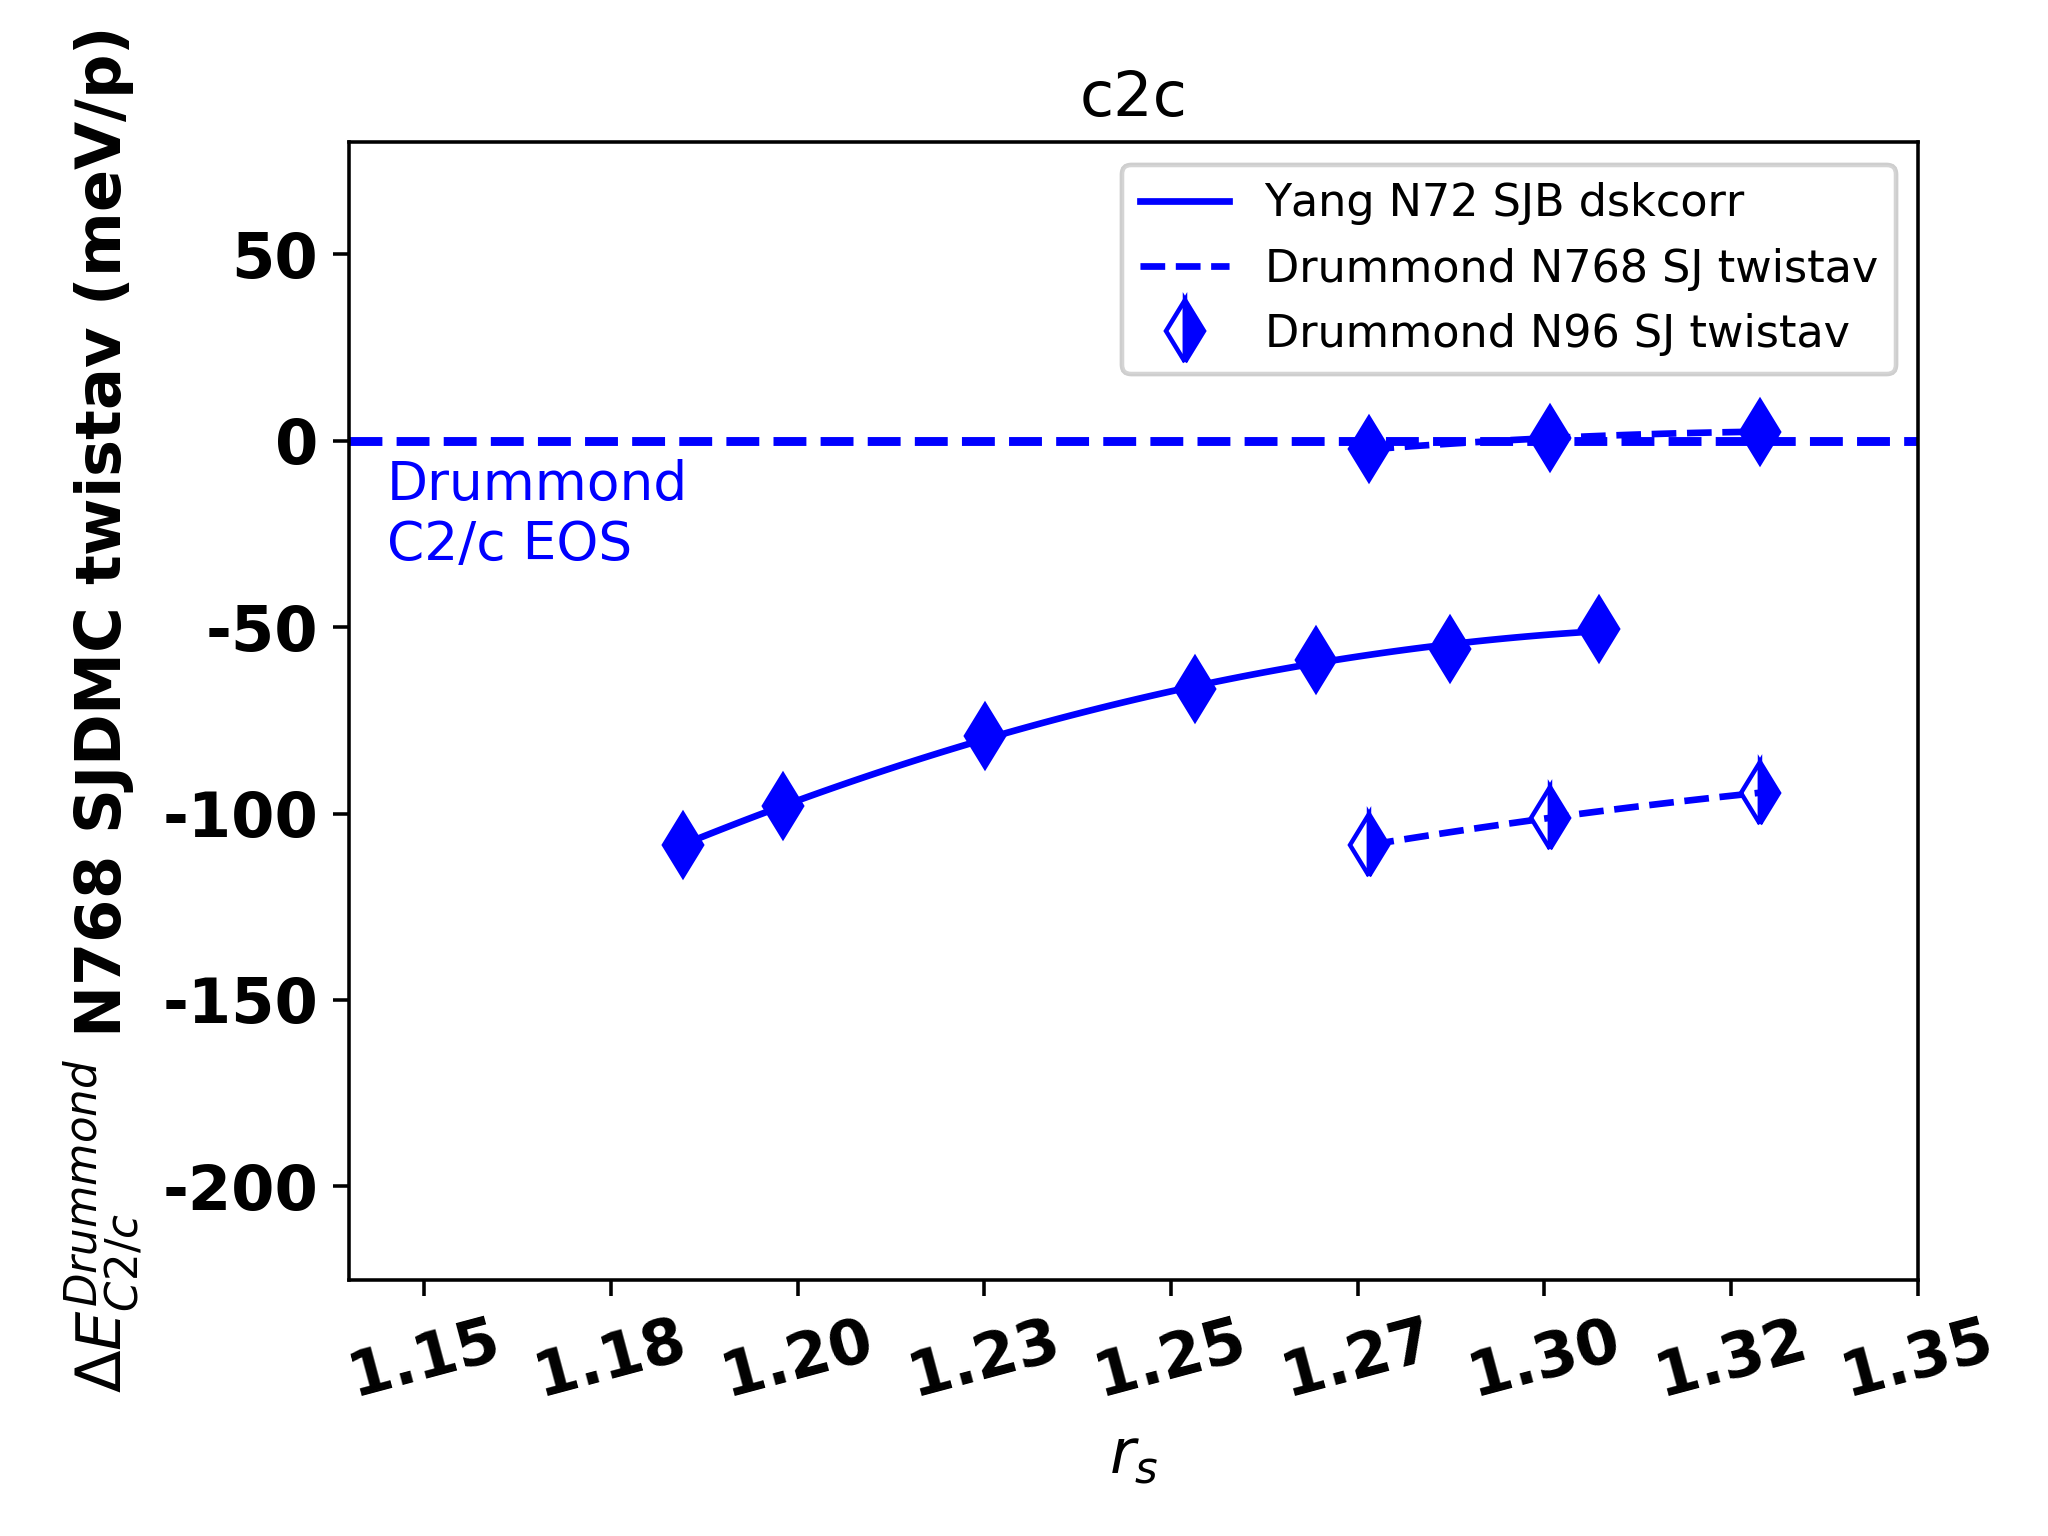
\includegraphics[scale=0.48]{006b_c2c_step0}
(a) DMC data.%\label{fig:static-c2c-yang-drummond-data}
\end{minipage}
%\begin{subfigure}{0.48\textwidth}
%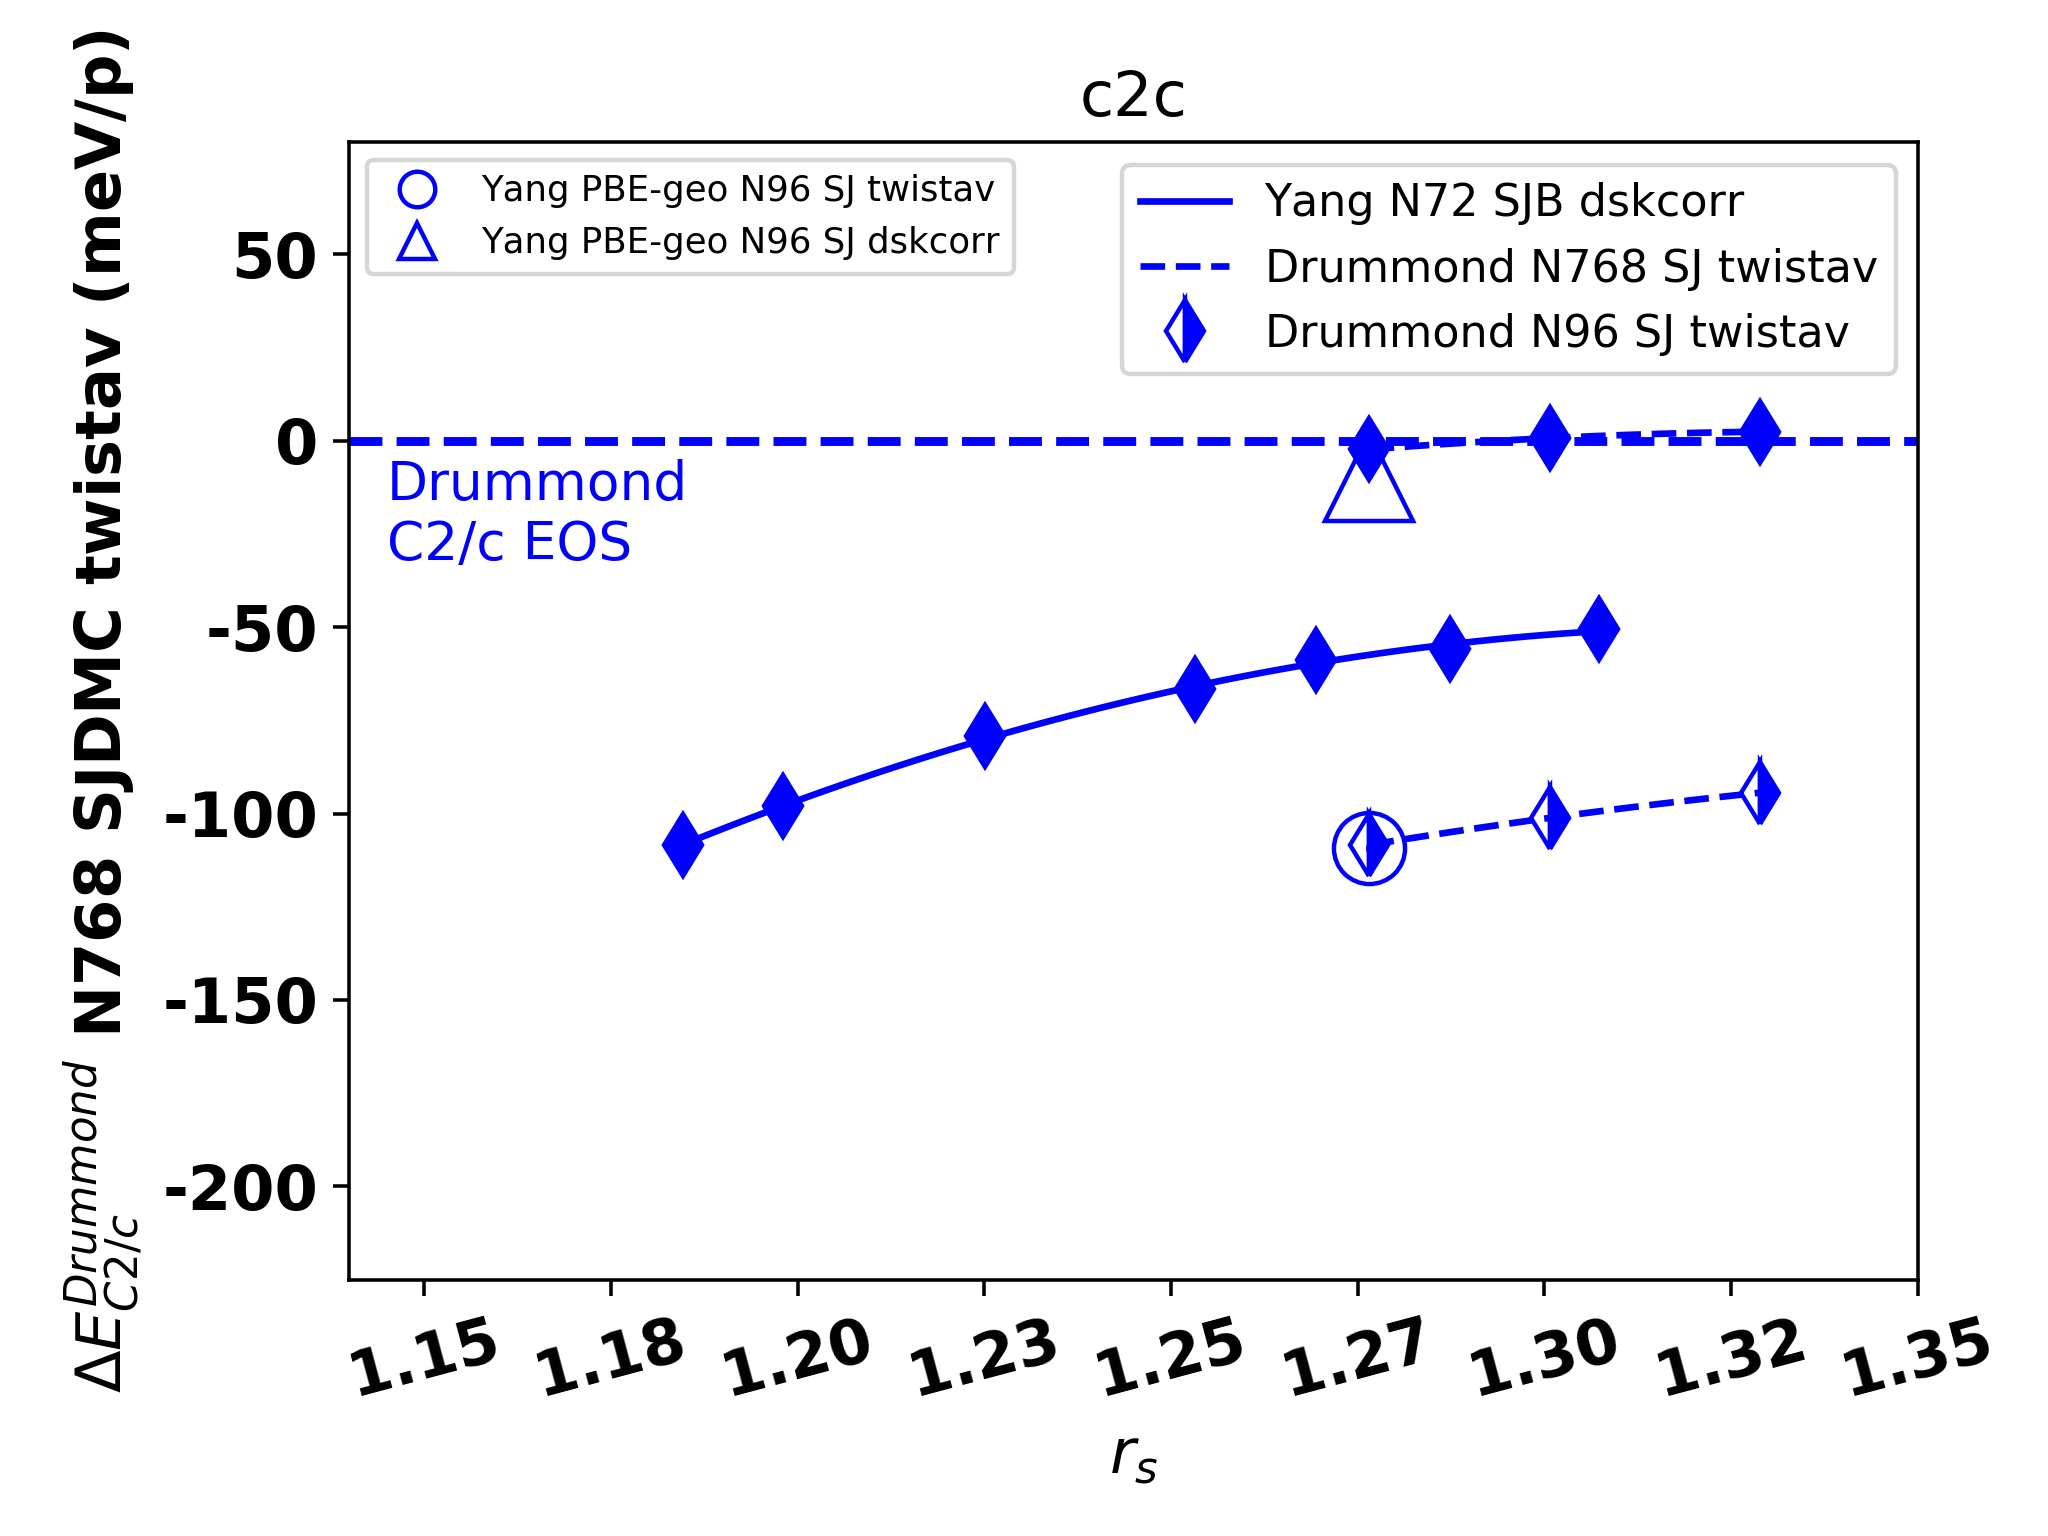
\includegraphics[scale=0.48]{figures/c2c/006b_c2c_step2}
%\caption{Reproduce PBE-geo N768 SJ twistav.\label{fig:static-c2c-yang-drummond-fs}}
%\end{subfigure}
%\begin{subfigure}{0.48\textwidth}
%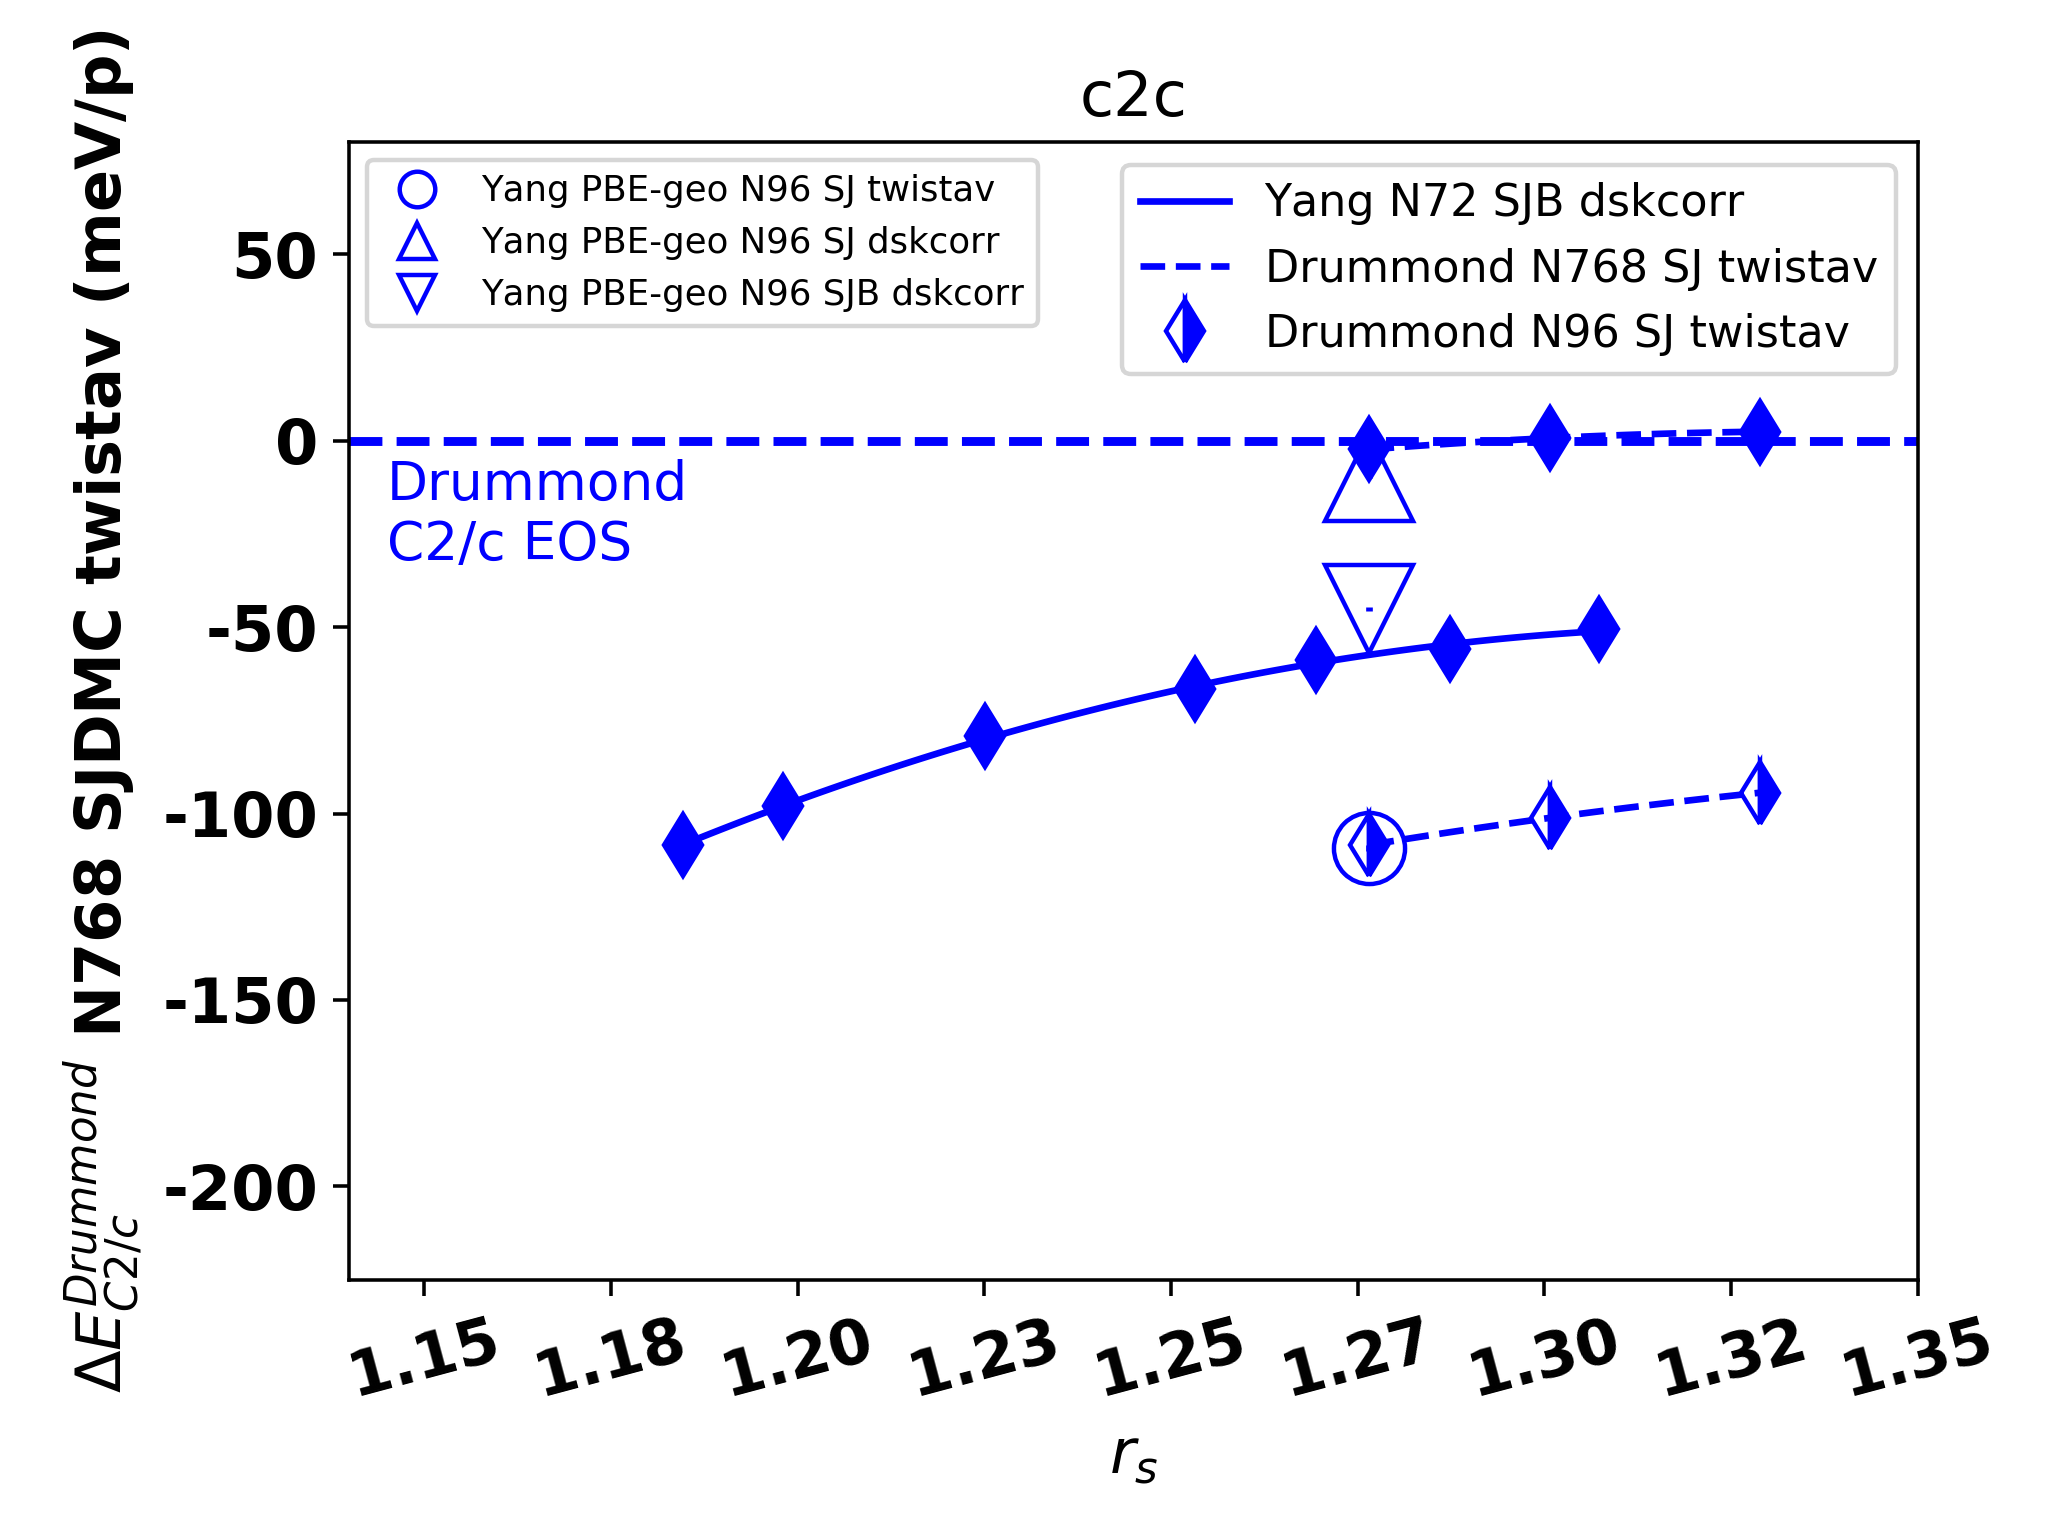
\includegraphics[scale=0.48]{figures/c2c/006b_c2c_step3}
%\caption{Effect of backflow.\label{fig:static-c2c-yang-drummond-bf}}
%\end{subfigure}
%\begin{subfigure}{0.48\textwidth}
%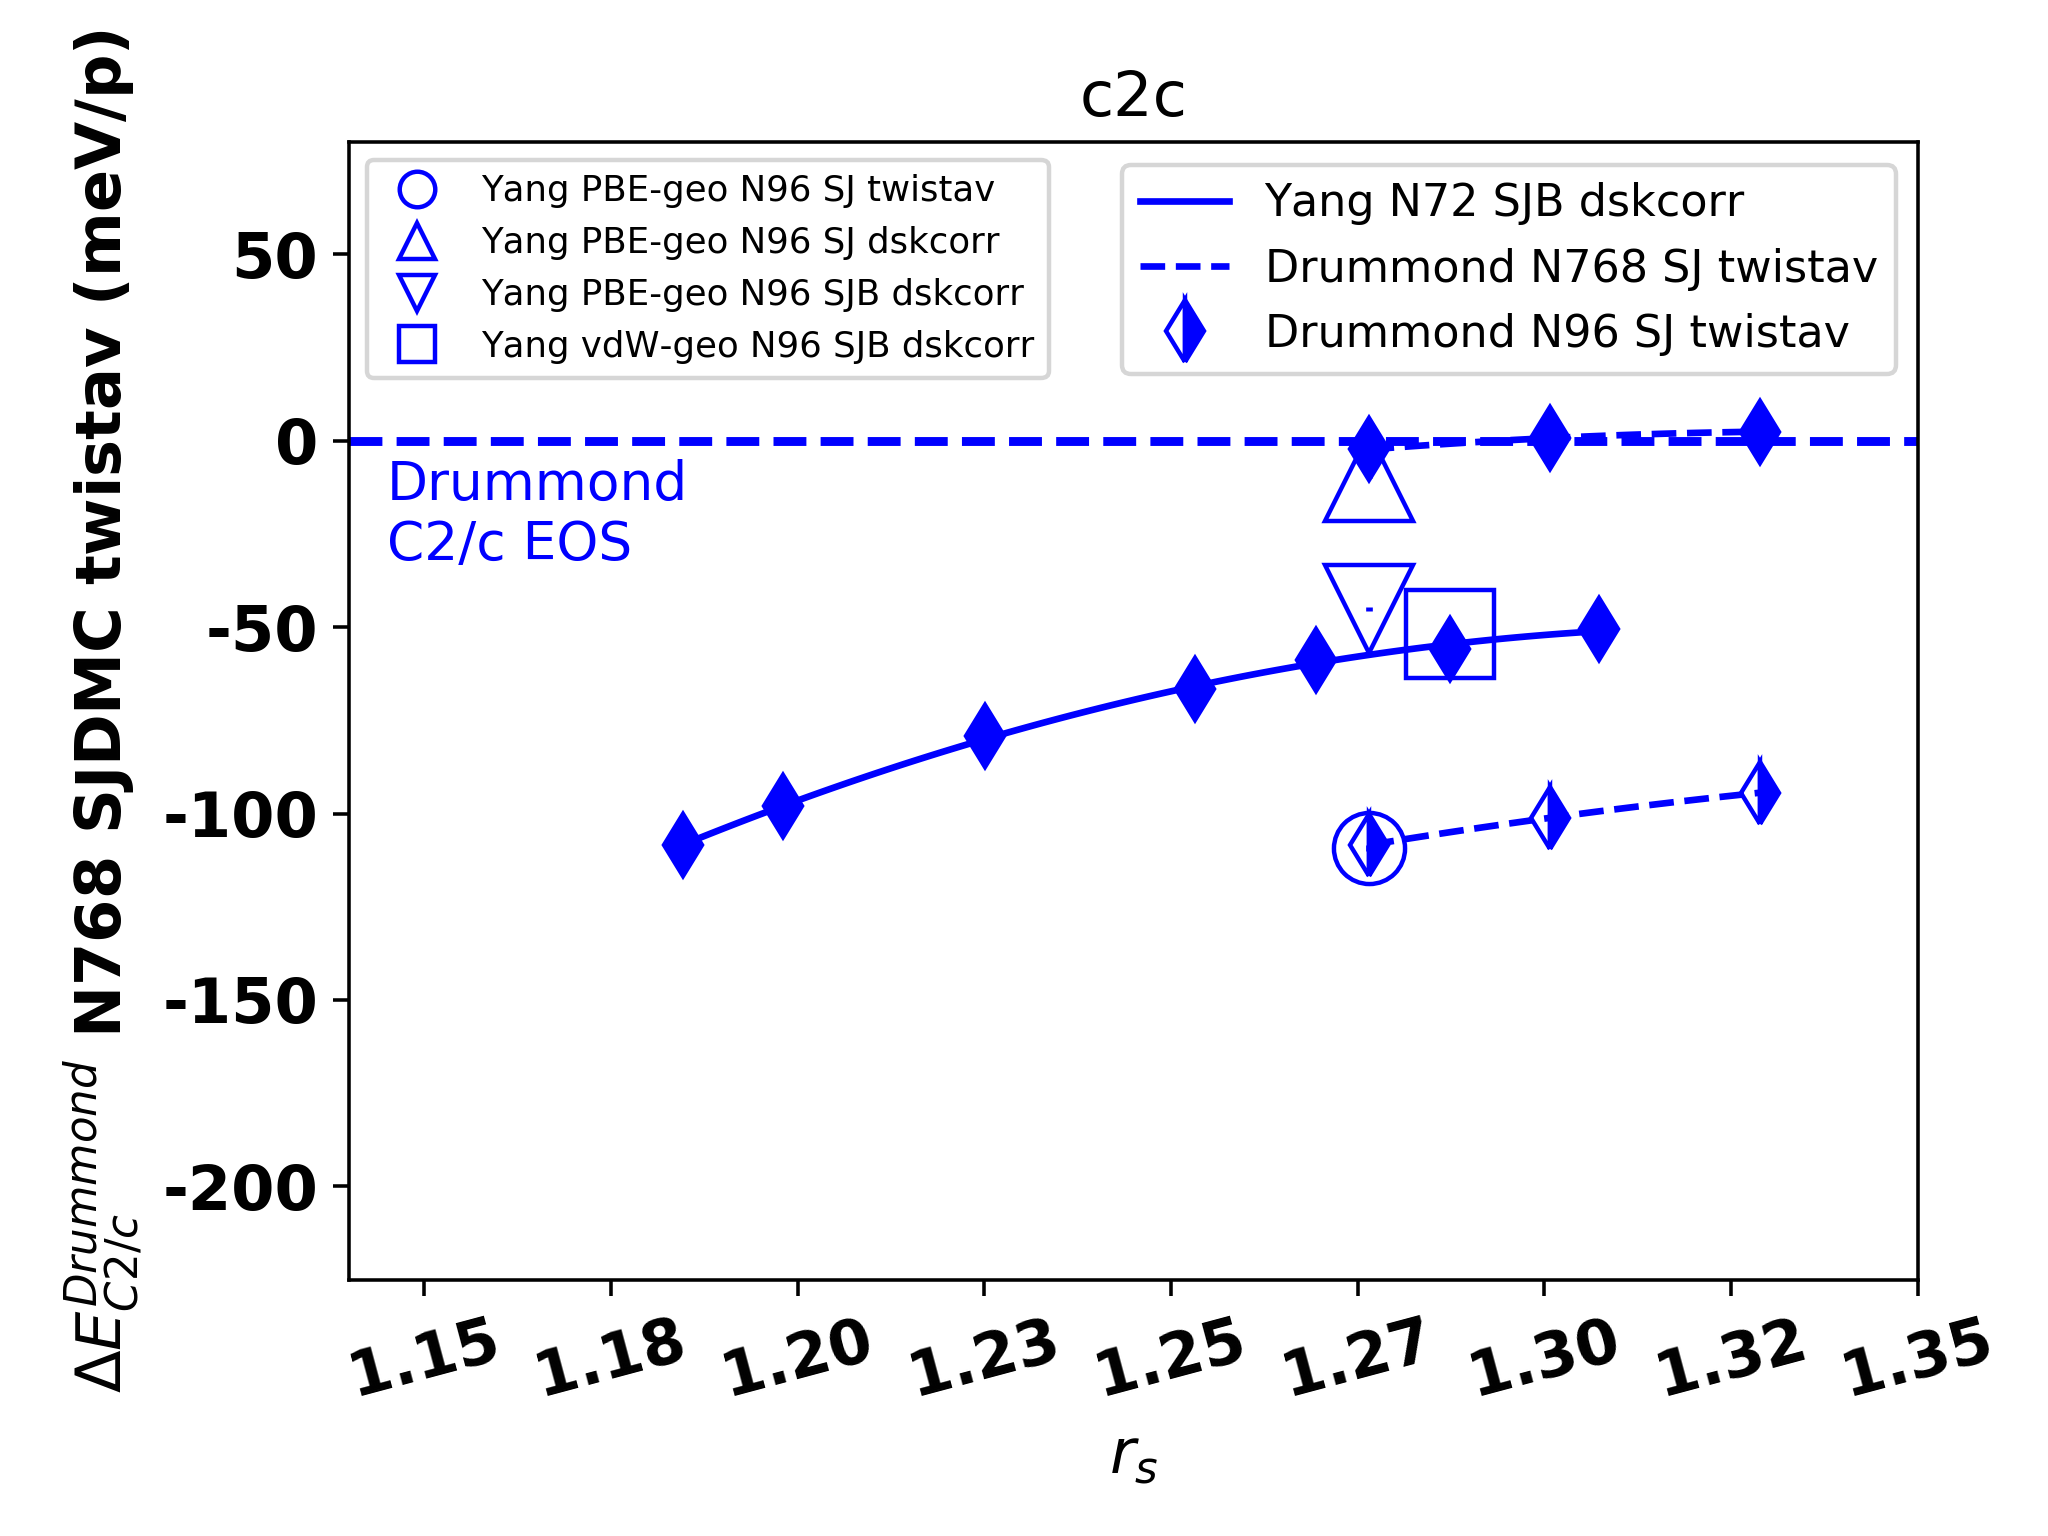
\includegraphics[scale=0.48]{figures/c2c/006b_c2c_step4}
%\caption{Effect of vdW-geo.\label{fig:static-c2c-yang-drummond-geo}}
%\end{subfigure}
\begin{minipage}{0.48\textwidth}
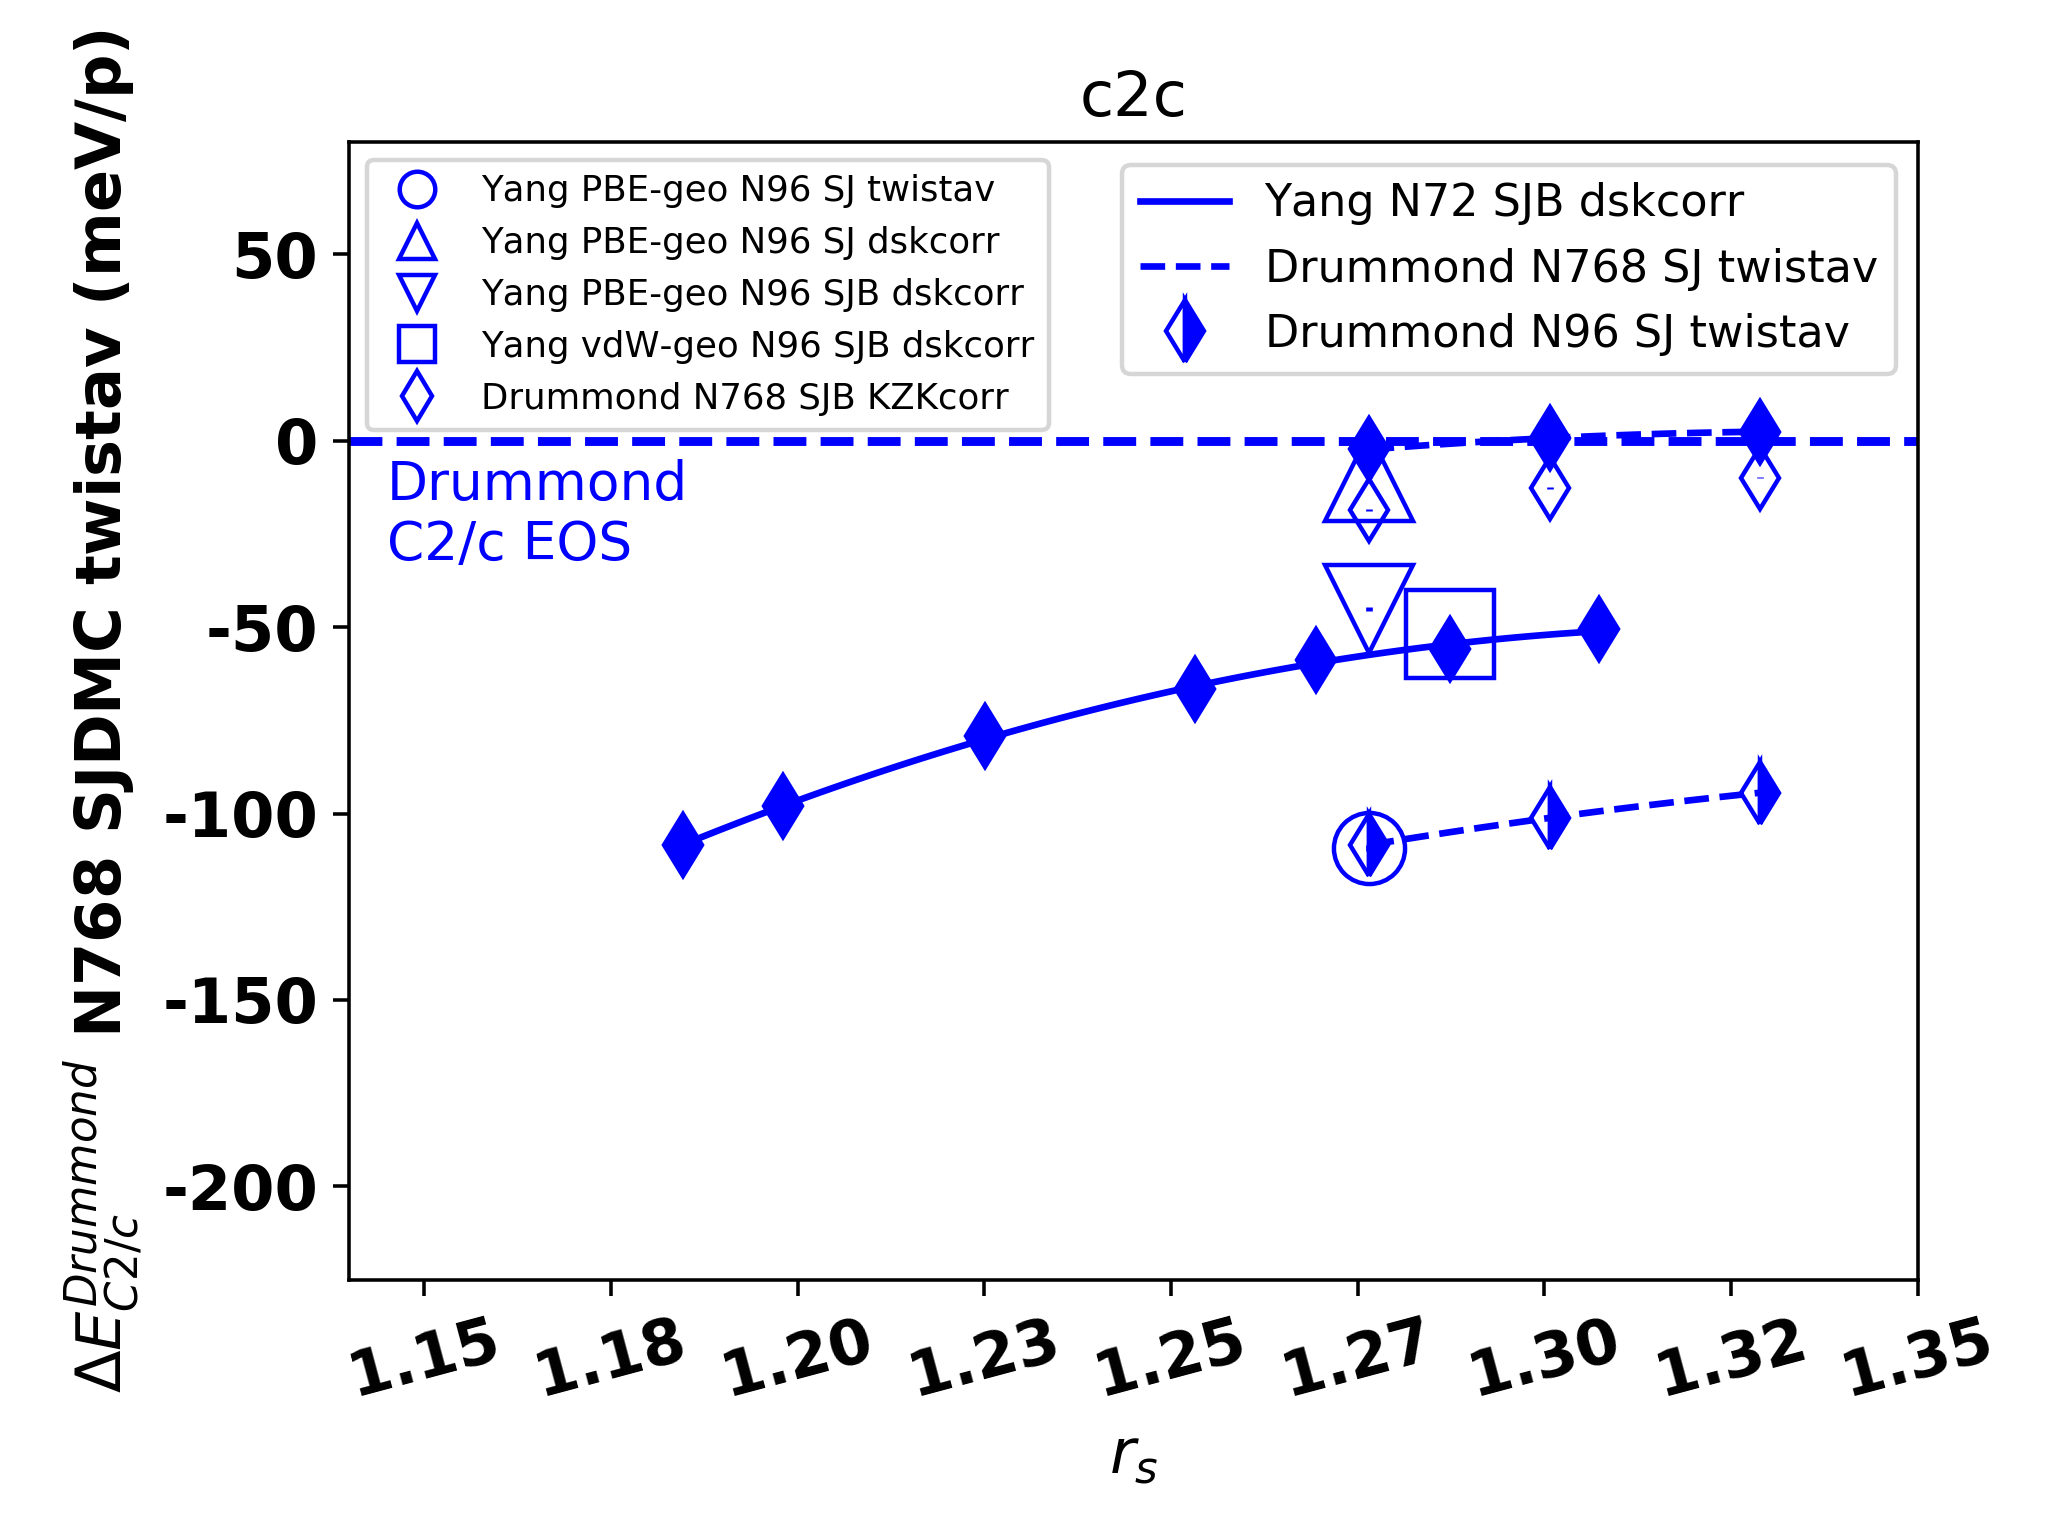
\includegraphics[scale=0.48]{006b_c2c_step5}
(b) Drummond SJB. %\label{fig:static-c2c-yang-drummond-last}
\end{minipage}
\caption{C2/c-24 DMC total energy relative to reference EOS.\label{fig:static-c2c-yang-drummond}}
\end{figure}

\subsection{Atomic Phase Candidate I4$_1$/amd}

Four sets of data are shown in Fig.~\ref{fig:static-i41amd-yang-mcminis-azadi}. A series of calculations are added in Fig.~\ref{fig:static-i41amd-yang-mcminis-azadi-data}-\ref{fig:static-i41amd-yang-mcminis-azadi-last} to connect them. Phase III EOS eqn.~\ref{eq:drum_sjdmc_n768} is again used as reference. The solid stars connected by a dot-dashed line are McMinis' SJ results. The solid stars connected by a dotted line are Azadi's FS-corrected results. The solid stars connected by a solid line are my results. Finally, the right-filled starts connected by dot-dashed lines are Azadi's N128 SJB twistav results without the Chiesa correction.

In Fig.~\ref{fig:static-i41amd-yang-mcminis-azadi-repro}, I attempt to reproduce Azadi's 128-atom results using QMCPACK (open stars). At $r_s=1.25$, our energies agree within 3 sigmas. However, at $r_s=1.17$, my energy is 18 meV/p higher than Azadi's. In Fig.~\ref{fig:static-i41amd-yang-mcminis-azadi-fs}, I add dskcorr to previous simulations and reproduce my N72 SJB energies (open downward triangles). In Fig.~\ref{fig:static-i41amd-yang-mcminis-azadi-last}, I remove back flow from previous simulations and obtain energies close to McMinis' results. At $r_s=1.17$, my N128 SJ dskcorr energy is 8(2) meV/p lower than McMinis'.

The difference between my N72 SJ dskcorr and McMinis' Ninf SJ energy is 8 meV/p. Assuming McMinis' energies are the correct thermodynamic values, then the remaining FS error after dskcorr is 8 meV/p. This is much lower than the remaining FS error in the molecular structures. Further, comparing the upward open triangles (SJ) and the downward open triangles (SJB), we see that back flow transformation gains $\sim$40 meV/p. Indeed, after shifting McMinis' energies by 48 meV/p (1.8 mha/p), our results agree well (Fig.~\ref{fig:static-enthalpy-vs-pressure}).

The 18 meV/p energy difference between mine and Azadi's twistav energies cannot be satisfactorily explained. Azadi used a different atomic structures than McMinis and myself. However, the energy variation caused by the structure difference should be no more than 5 meV/p.

%\begin{figure}[h]
%\begin{subfigure}{0.48\textwidth}
%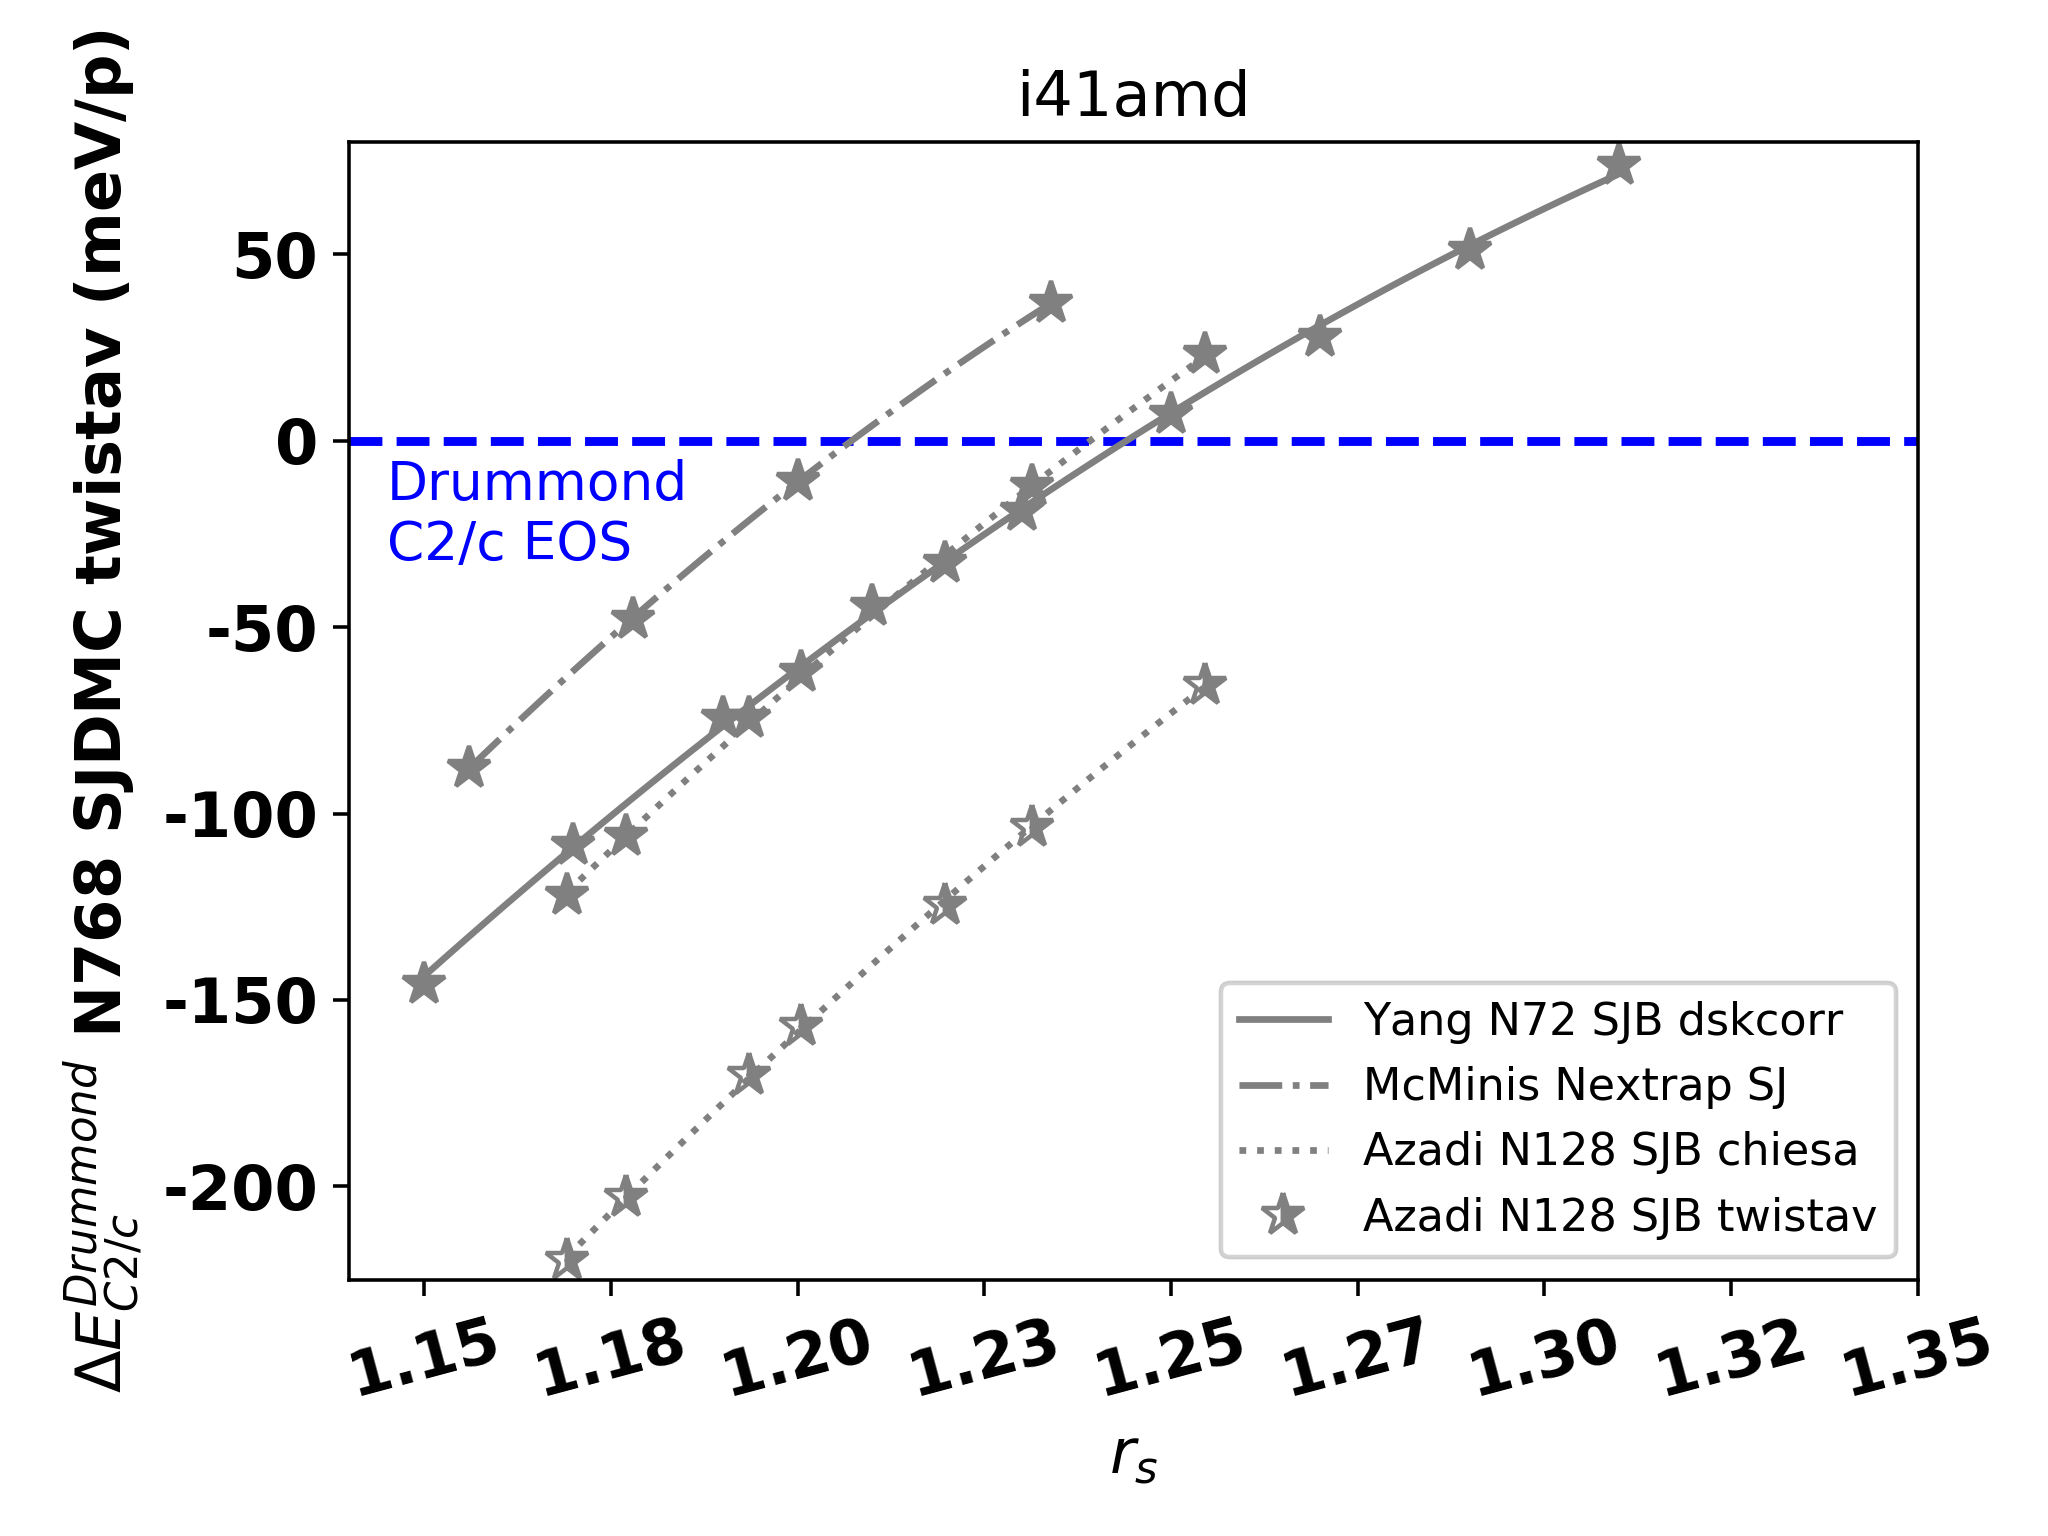
\includegraphics[scale=0.48]{figures/i41amd/006b_i41amd_step0}
%\caption{DMC data.\label{fig:static-i41amd-yang-mcminis-azadi-data}}
%\end{subfigure}
%\begin{subfigure}{0.48\textwidth}
%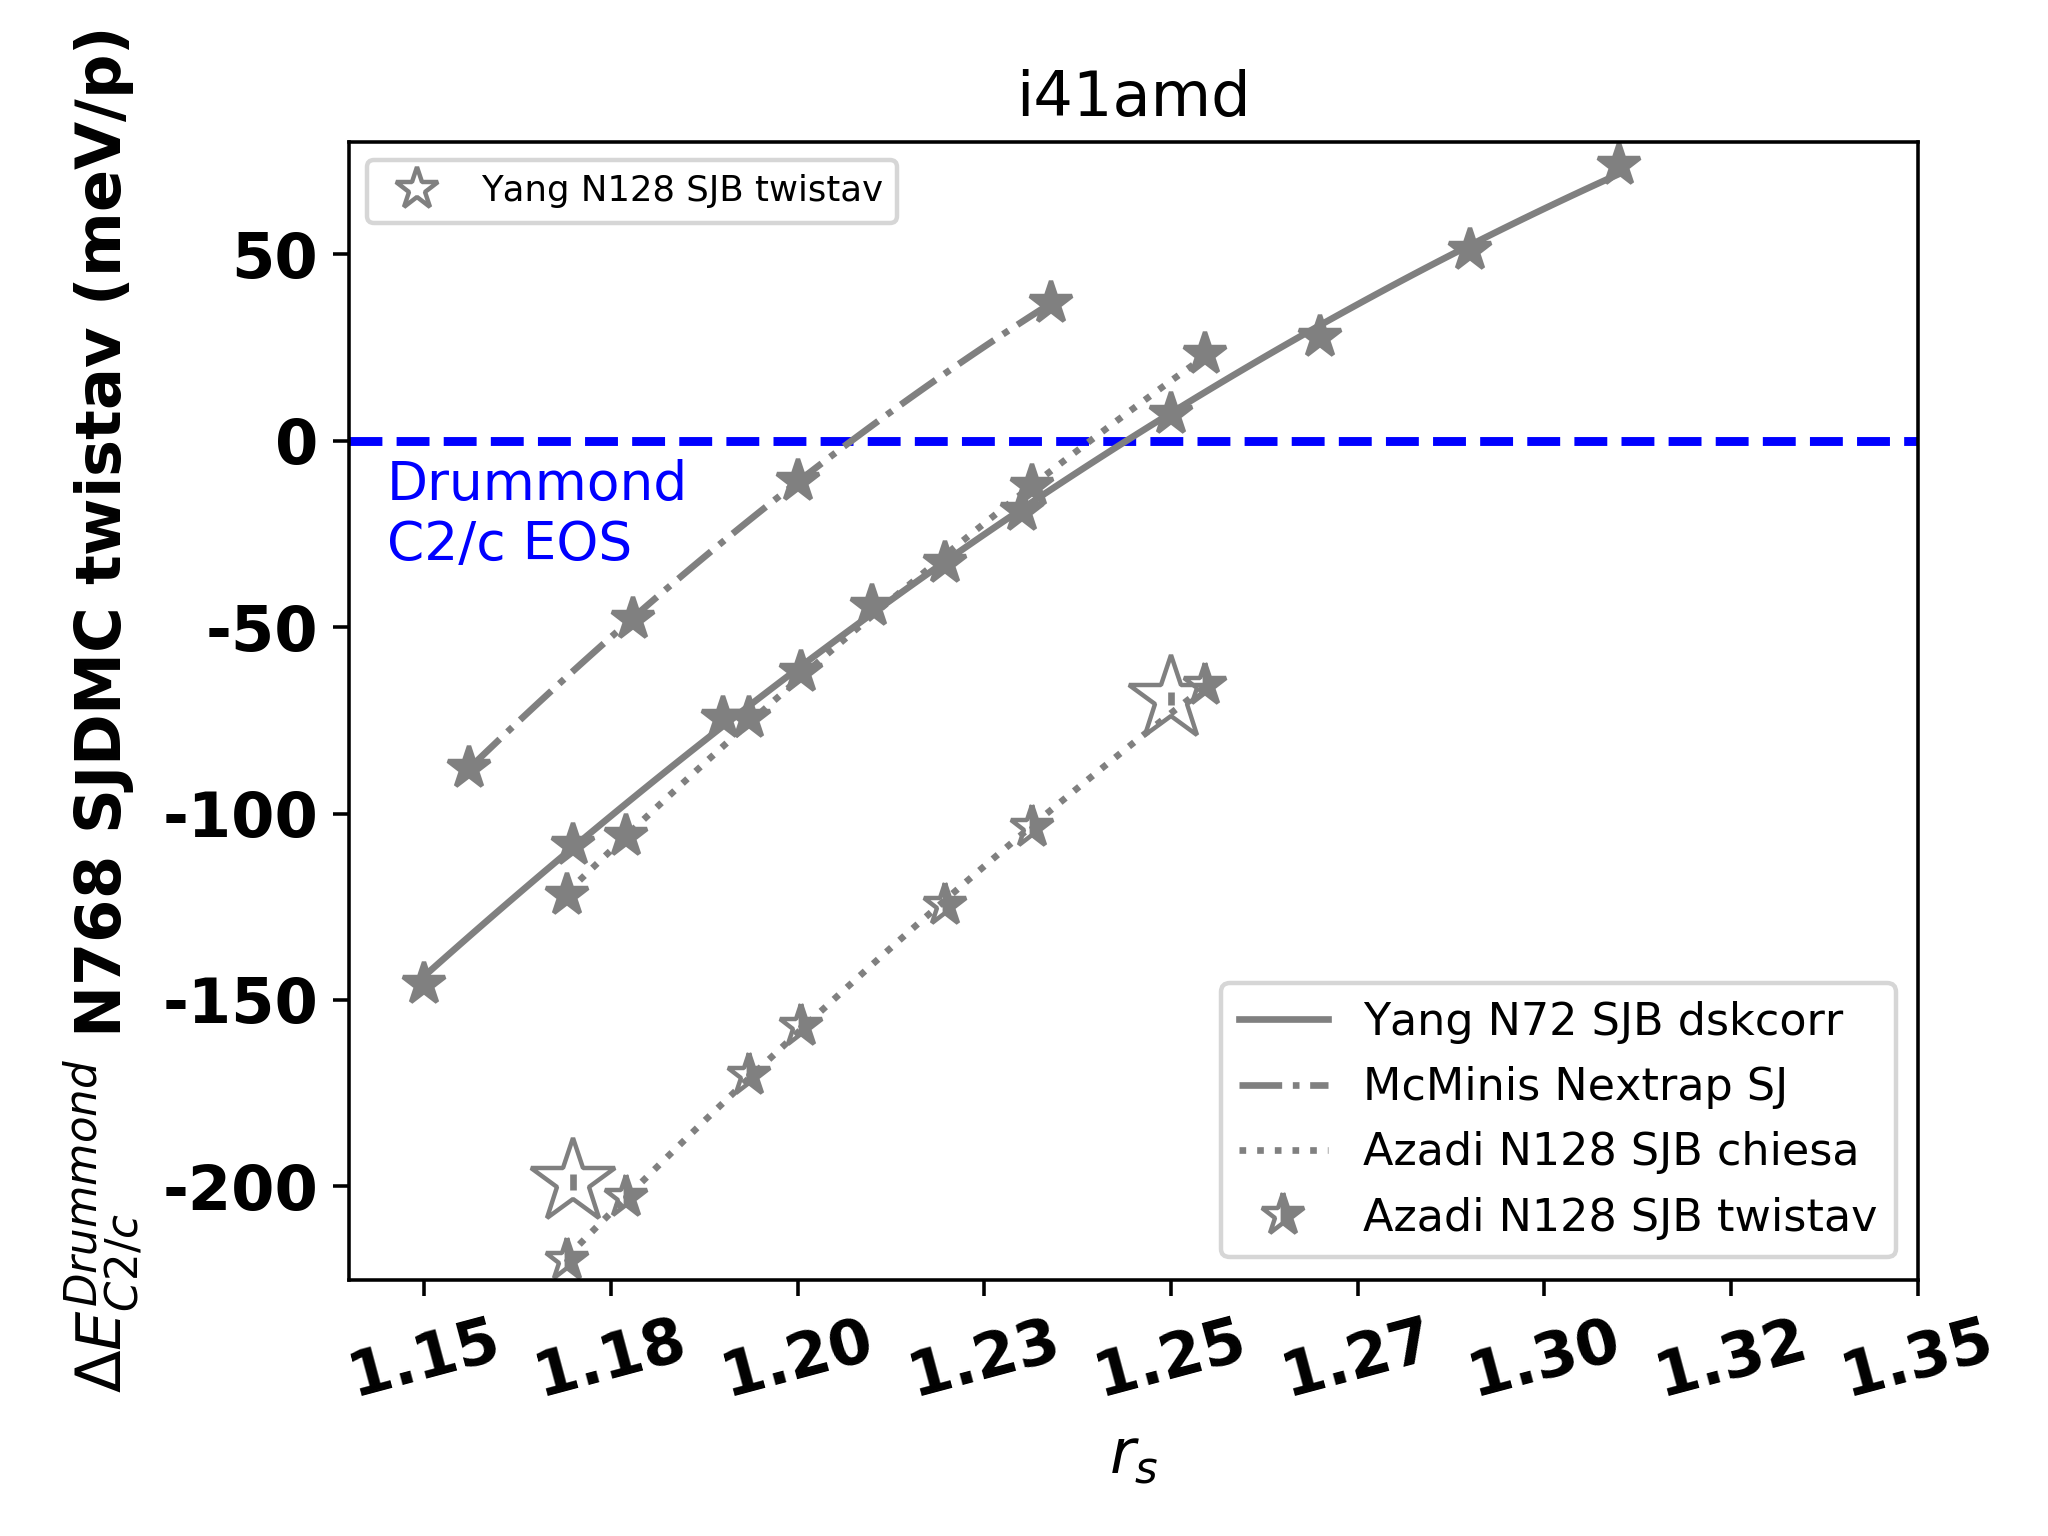
\includegraphics[scale=0.48]{figures/i41amd/006b_i41amd_step1}
%\caption{Reproduce PBE-geo N128 SJB twistav.\label{fig:static-i41amd-yang-mcminis-azadi-repro}}
%\end{subfigure}
%\begin{subfigure}{0.48\textwidth}
%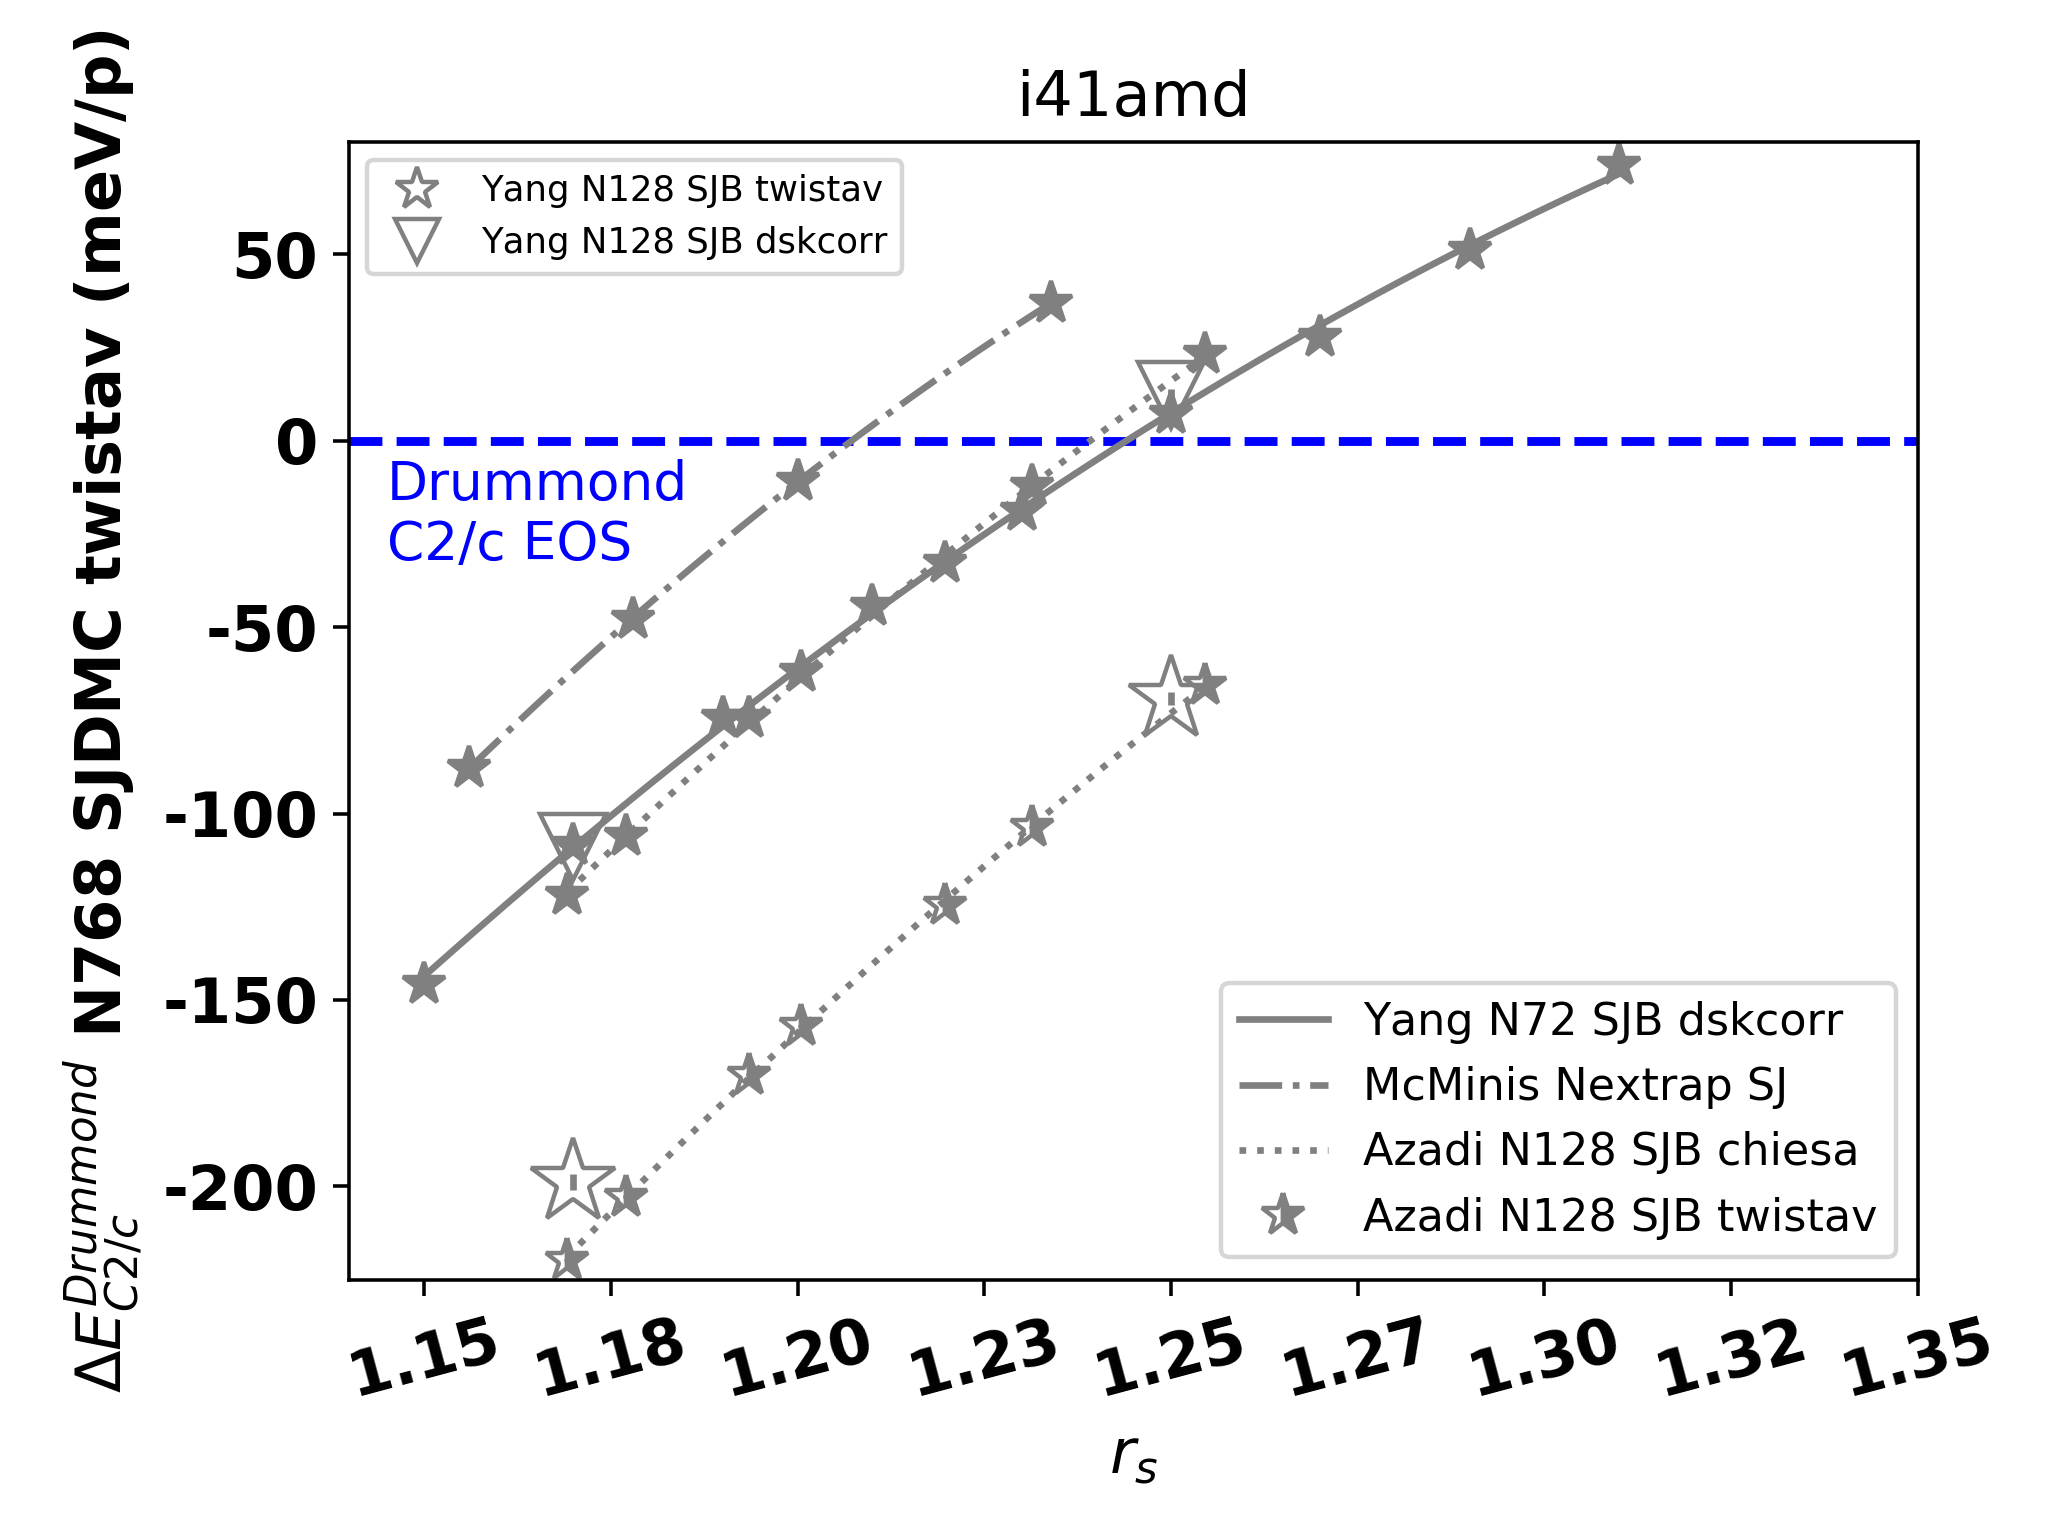
\includegraphics[scale=0.48]{figures/i41amd/006b_i41amd_step2}
%\caption{Match N96 and N72 using dskcorr.\label{fig:static-i41amd-yang-mcminis-azadi-fs}}
%\end{subfigure}
%\begin{subfigure}{0.48\textwidth}
%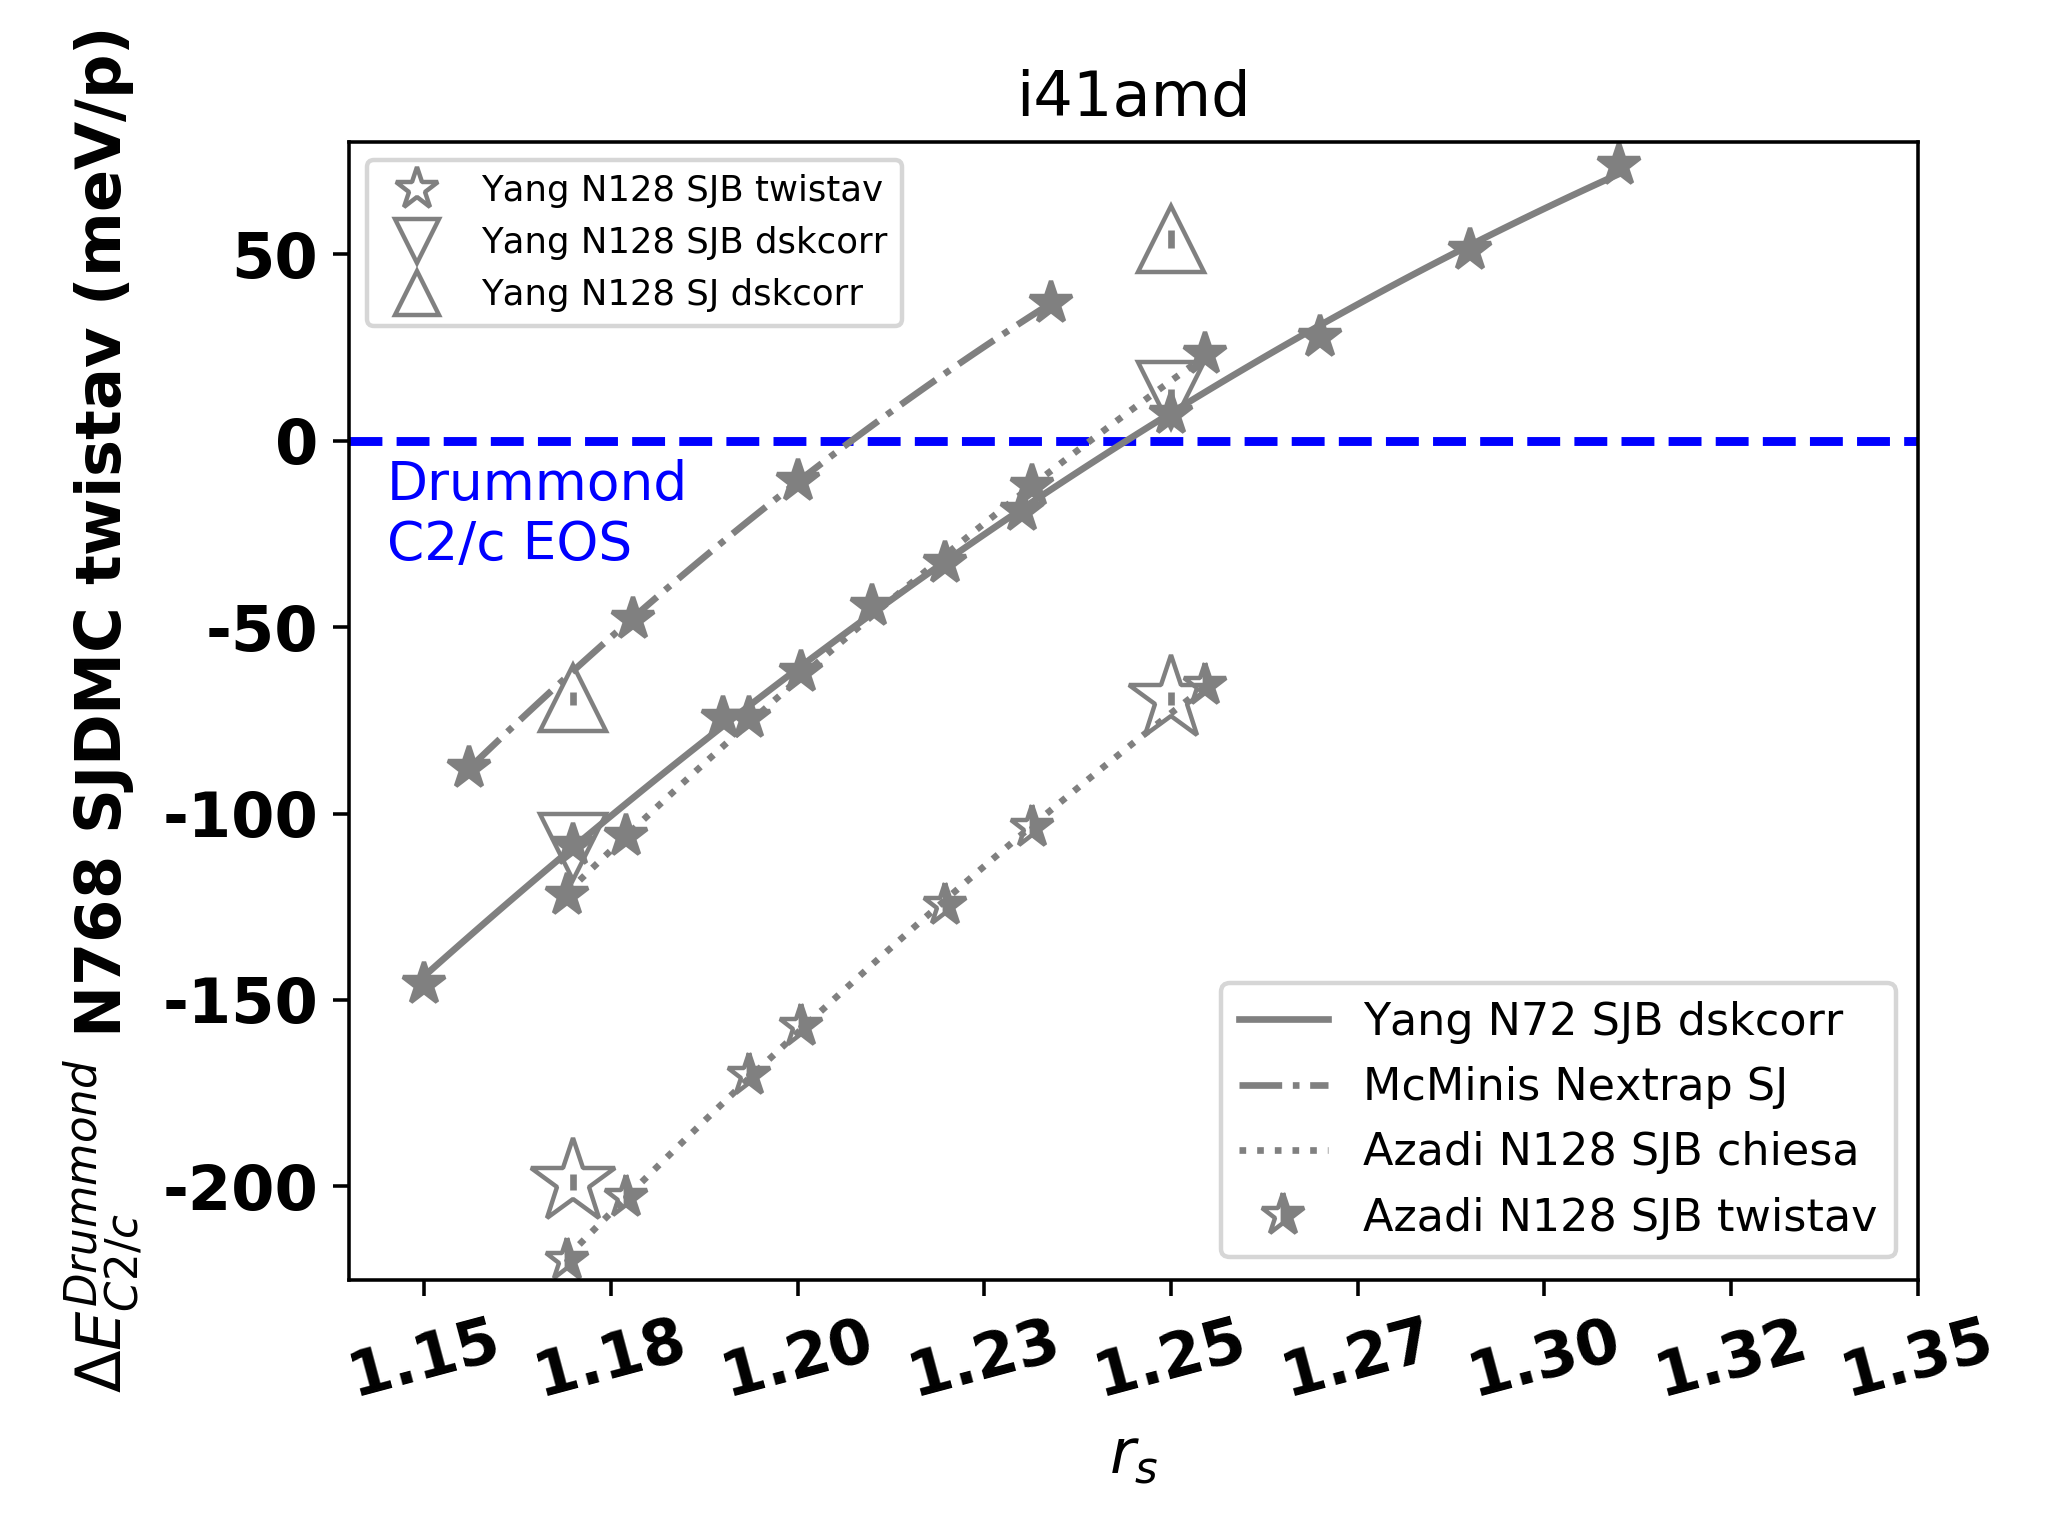
\includegraphics[scale=0.48]{figures/i41amd/006b_i41amd_step3}
%\caption{Reproduce McMinis SJ.\label{fig:static-i41amd-yang-mcminis-azadi-last}}
%\end{subfigure}
%\caption{I4$_1$/amd\label{fig:static-i41amd-yang-mcminis-azadi}}
%\end{figure}

\subsection{Molecular Candidate Cmca-4}

Three sets of data are shown in Fig.~\ref{fig:static-cmca4-yang-drummond-azadi}. The same reference EOS eq.~(\ref{eq:drum_sjdmc_n768}) is used as before. The solid downward triangles connected by a dashed line are Drummond N768 SJ twistav results. The solid downward triangles connected by a dotted line are Azadi's N128 SJB chiesa results [Azadi2014SI]. Finally, the solid downward triangles connected by a solid line are my N72 SJB dskcorr results.

In Fig.~\ref{fig:static-cmca4-yang-drummond-azadi-kzk}, KZKcorr=13-14 meV/p is added to Drummond SJ results to produce the top-filled downward triangles. In Fig.~\ref{fig:static-cmca4-yang-drummond-azadi-sjb}, Drummond's back flow results, corrected by KZKcorr, are shown as open downward triangles. At $r_s=1.30$ my SBJ dskcorr energy is lower than Drummond's SBJ KZKcorr energy by \textbf{37 meV/p}.

Azadi's SJB results are more consistent with Drummond's SJ results than SJB results. This discrepancy is unlikely to be due to the Chiesa correction because the remaining FS error after the Chiesa correction is usually negative.

\begin{figure}[h]
\begin{minipage}{0.48\textwidth}
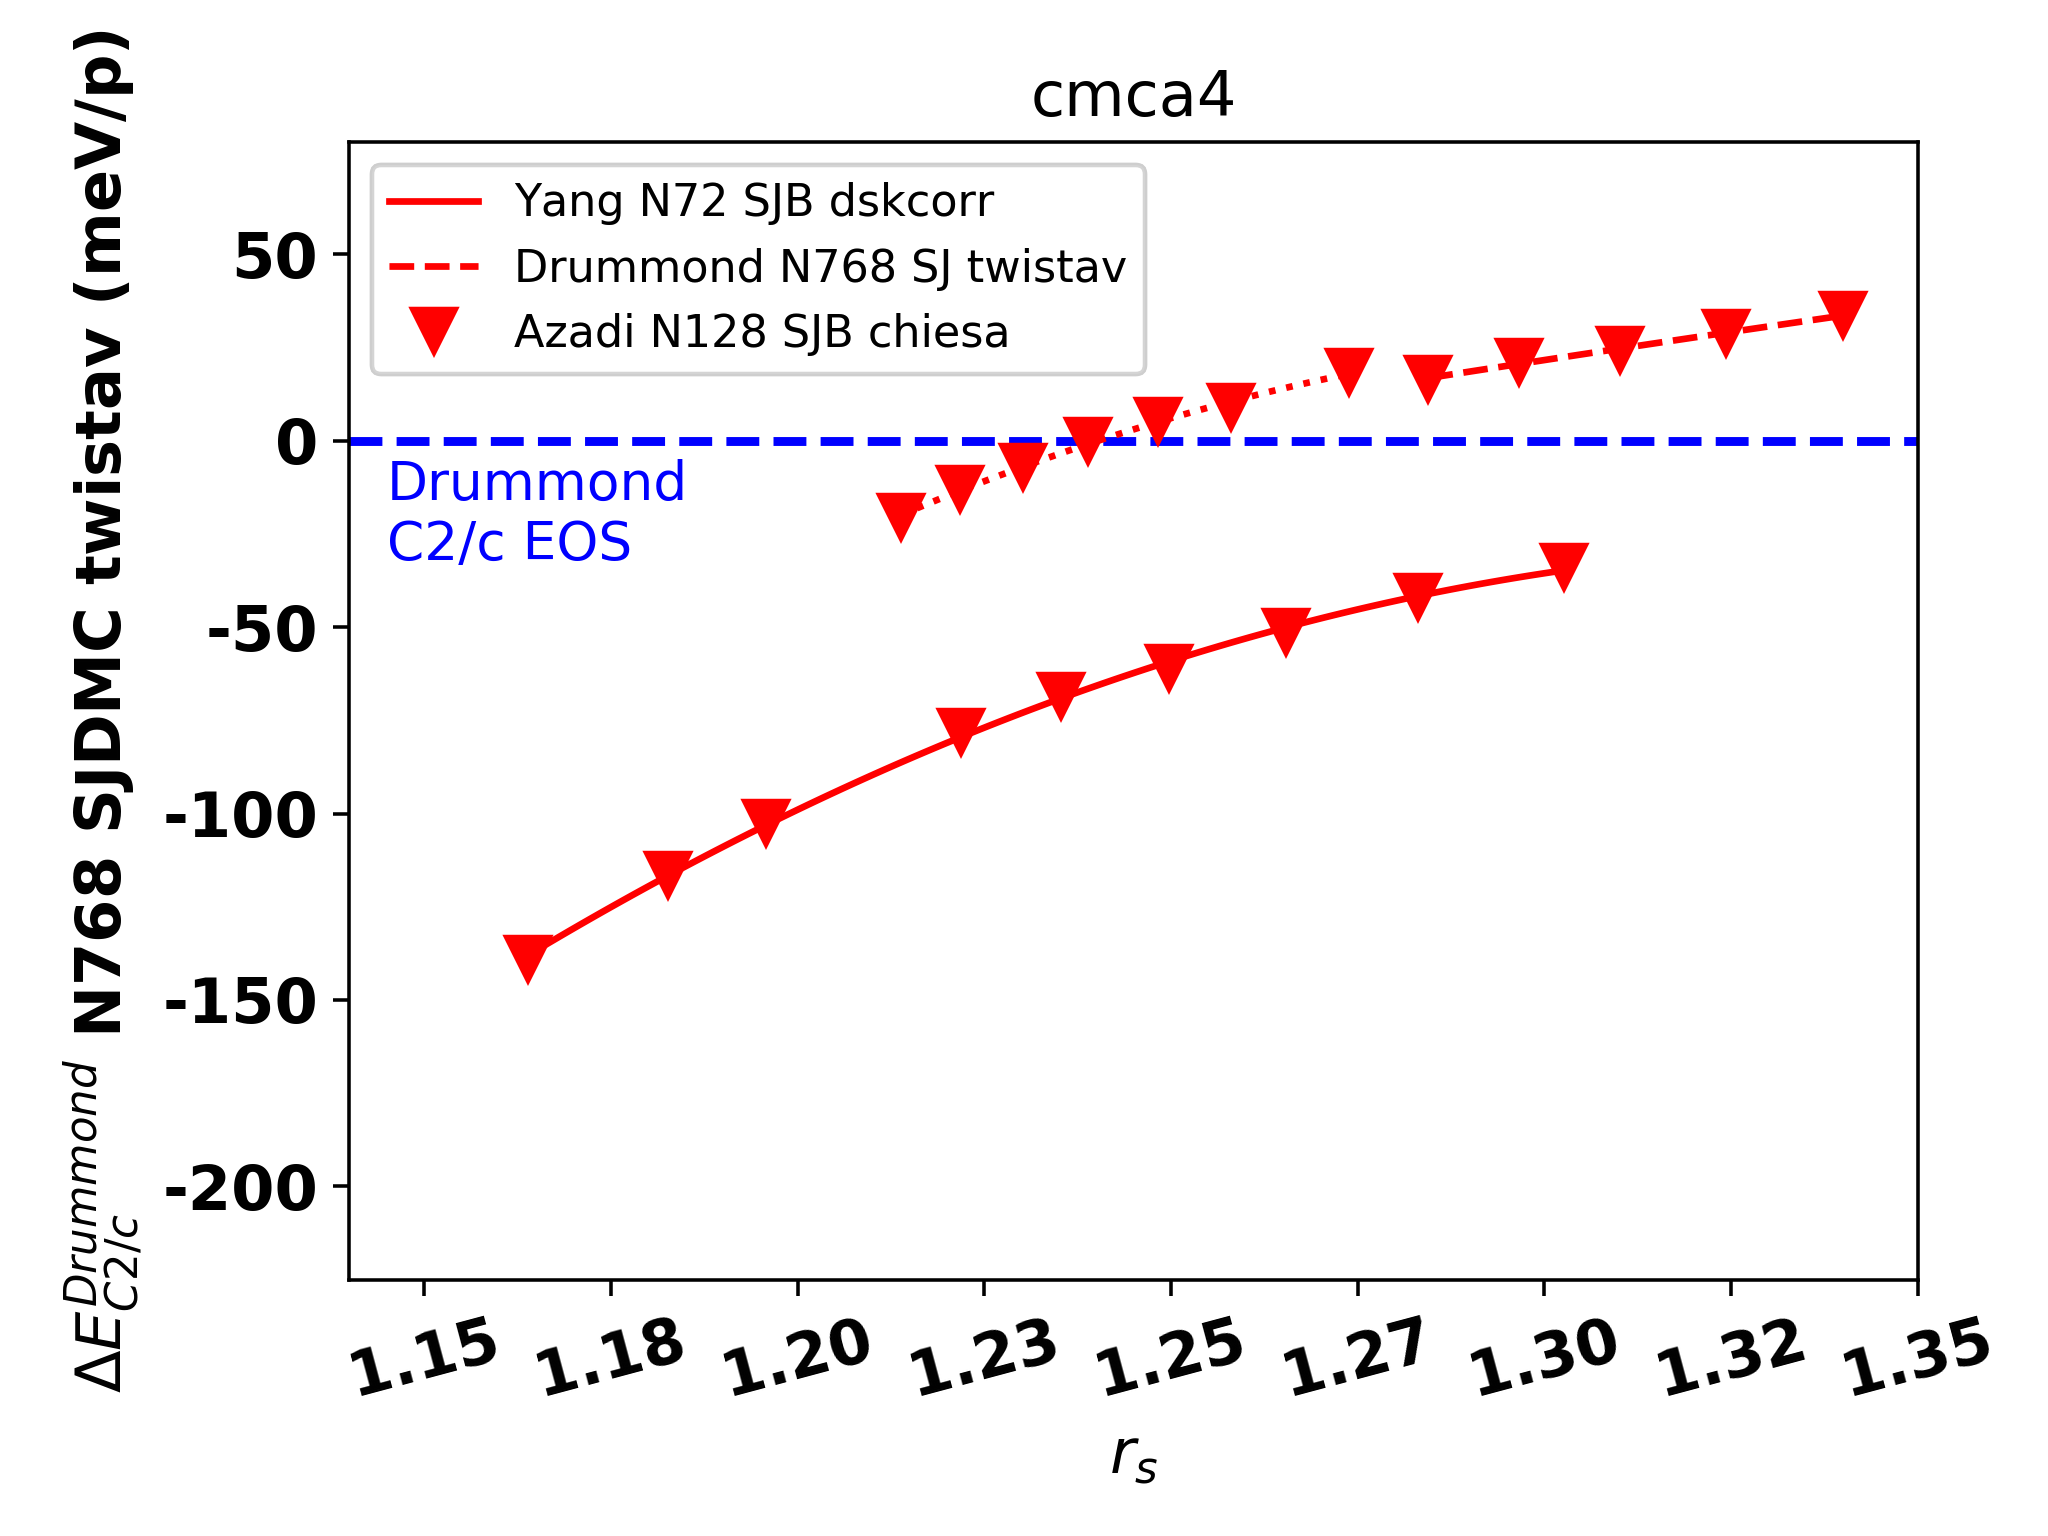
\includegraphics[width=\columnwidth]{006b_cmca4_step0}
 (a) DMC data.%\label{fig:static-cmca4-yang-drummond-azadi-data}
\end{minipage}
%\begin{subfigure}{0.48\textwidth}
%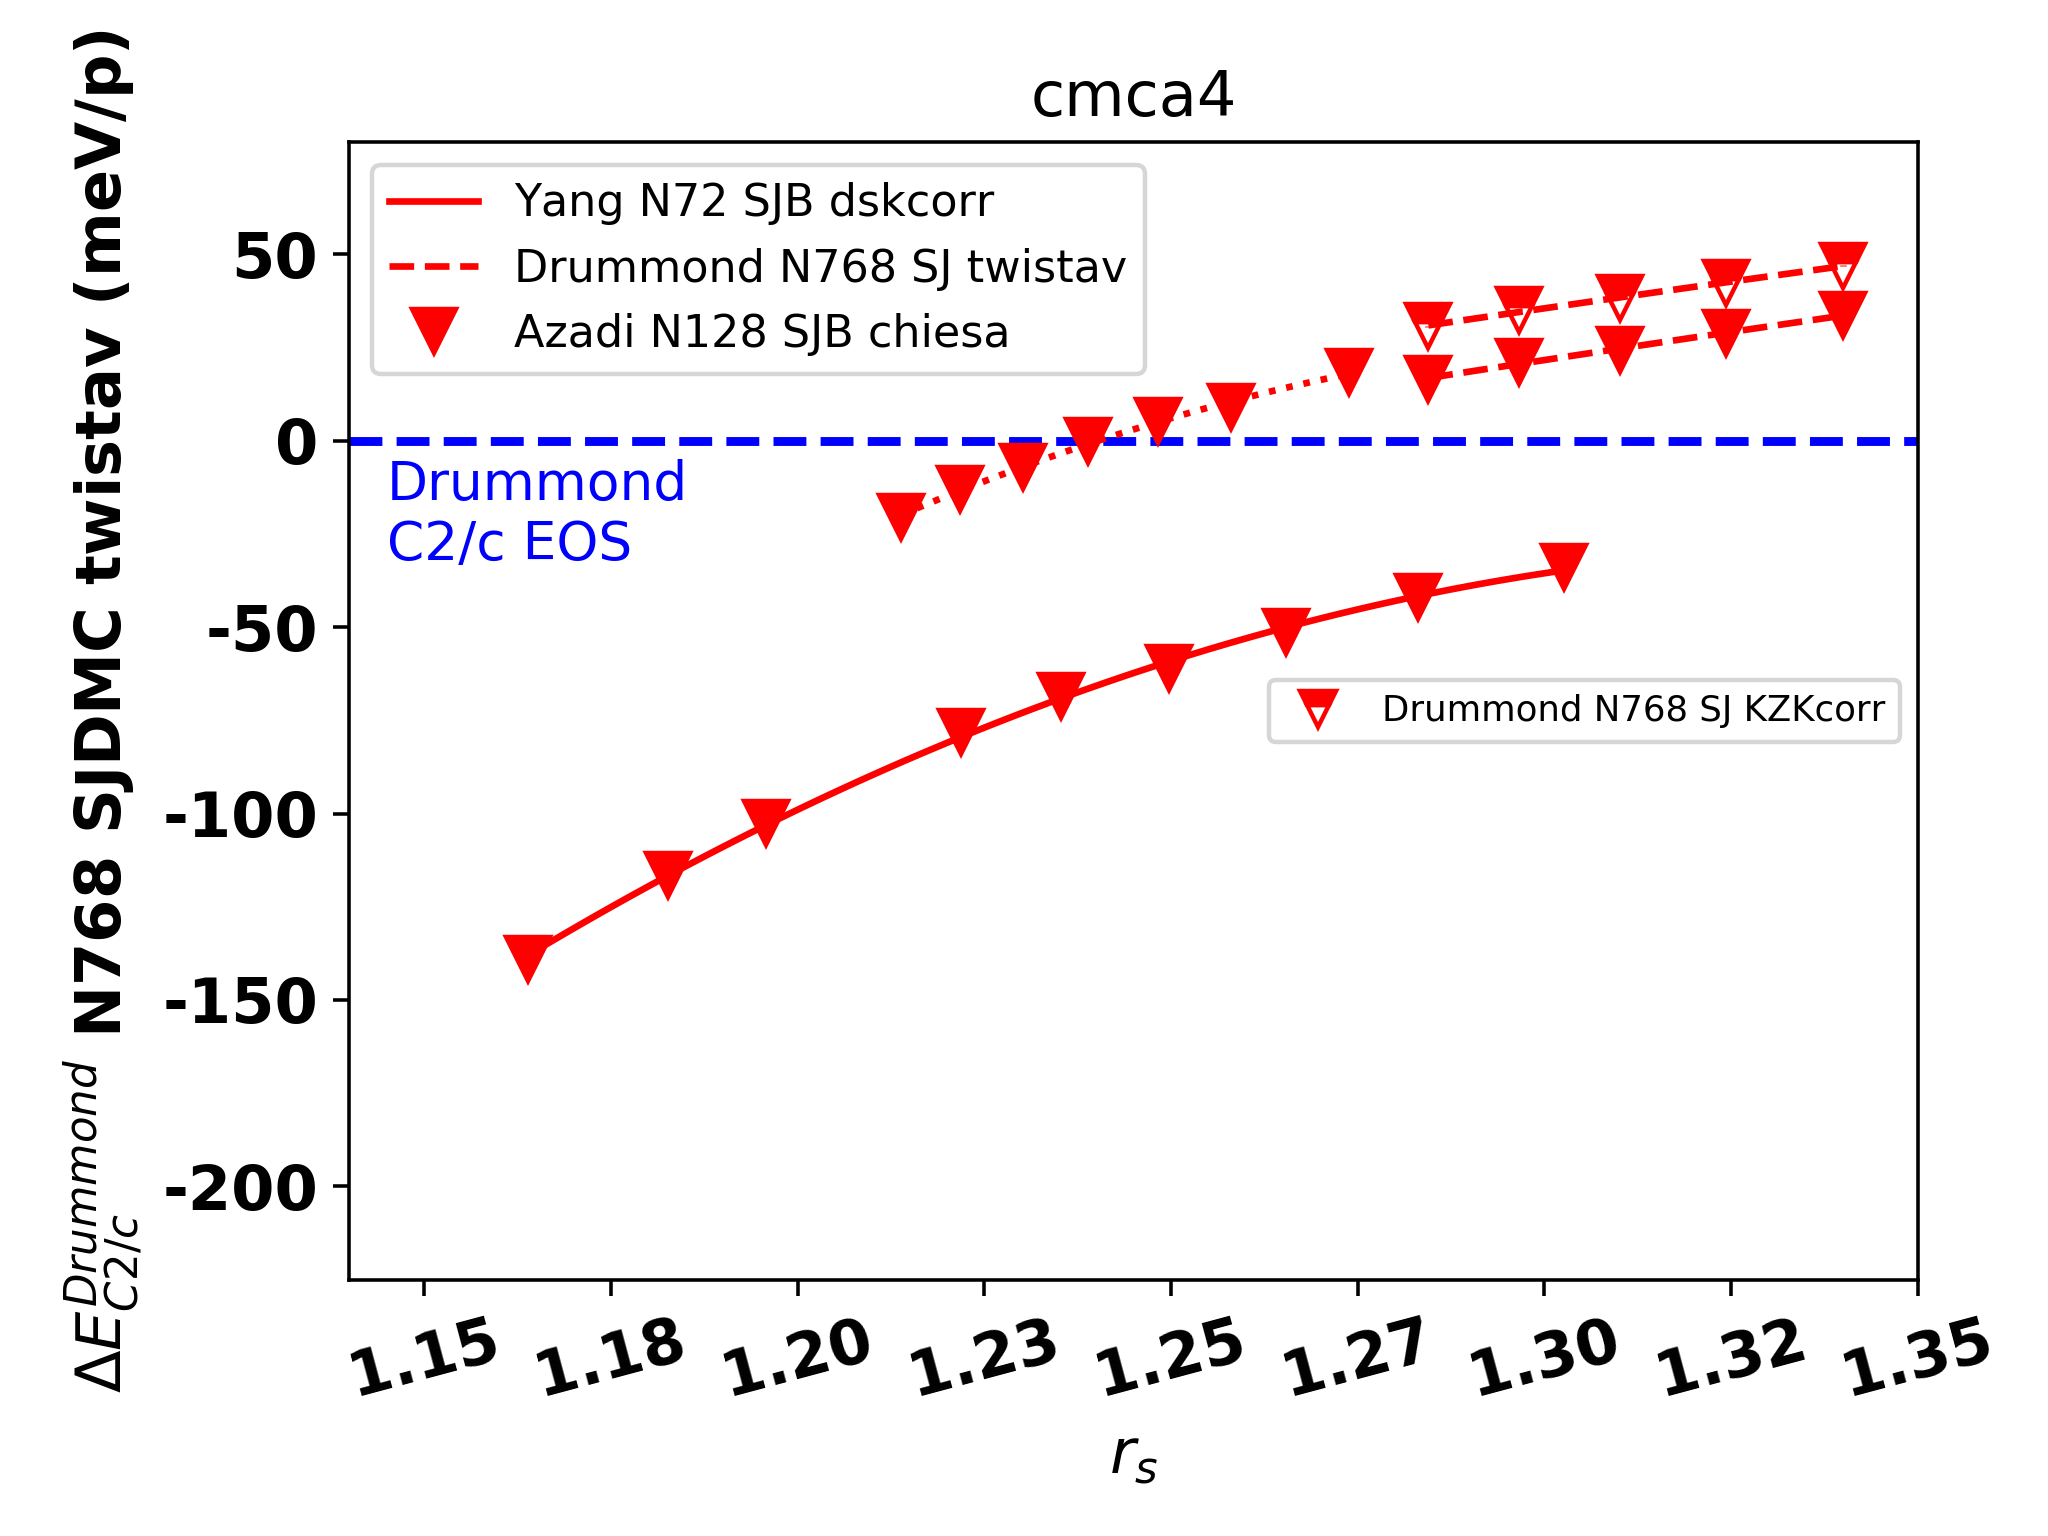
\includegraphics[scale=0.48]{figures/cmca4/006b_cmca4_step1}
%\caption{Add KZKcorr to Drummond.\label{fig:static-cmca4-yang-drummond-azadi-kzk}}
%\end{subfigure}
\begin{minipage}{0.48\textwidth}
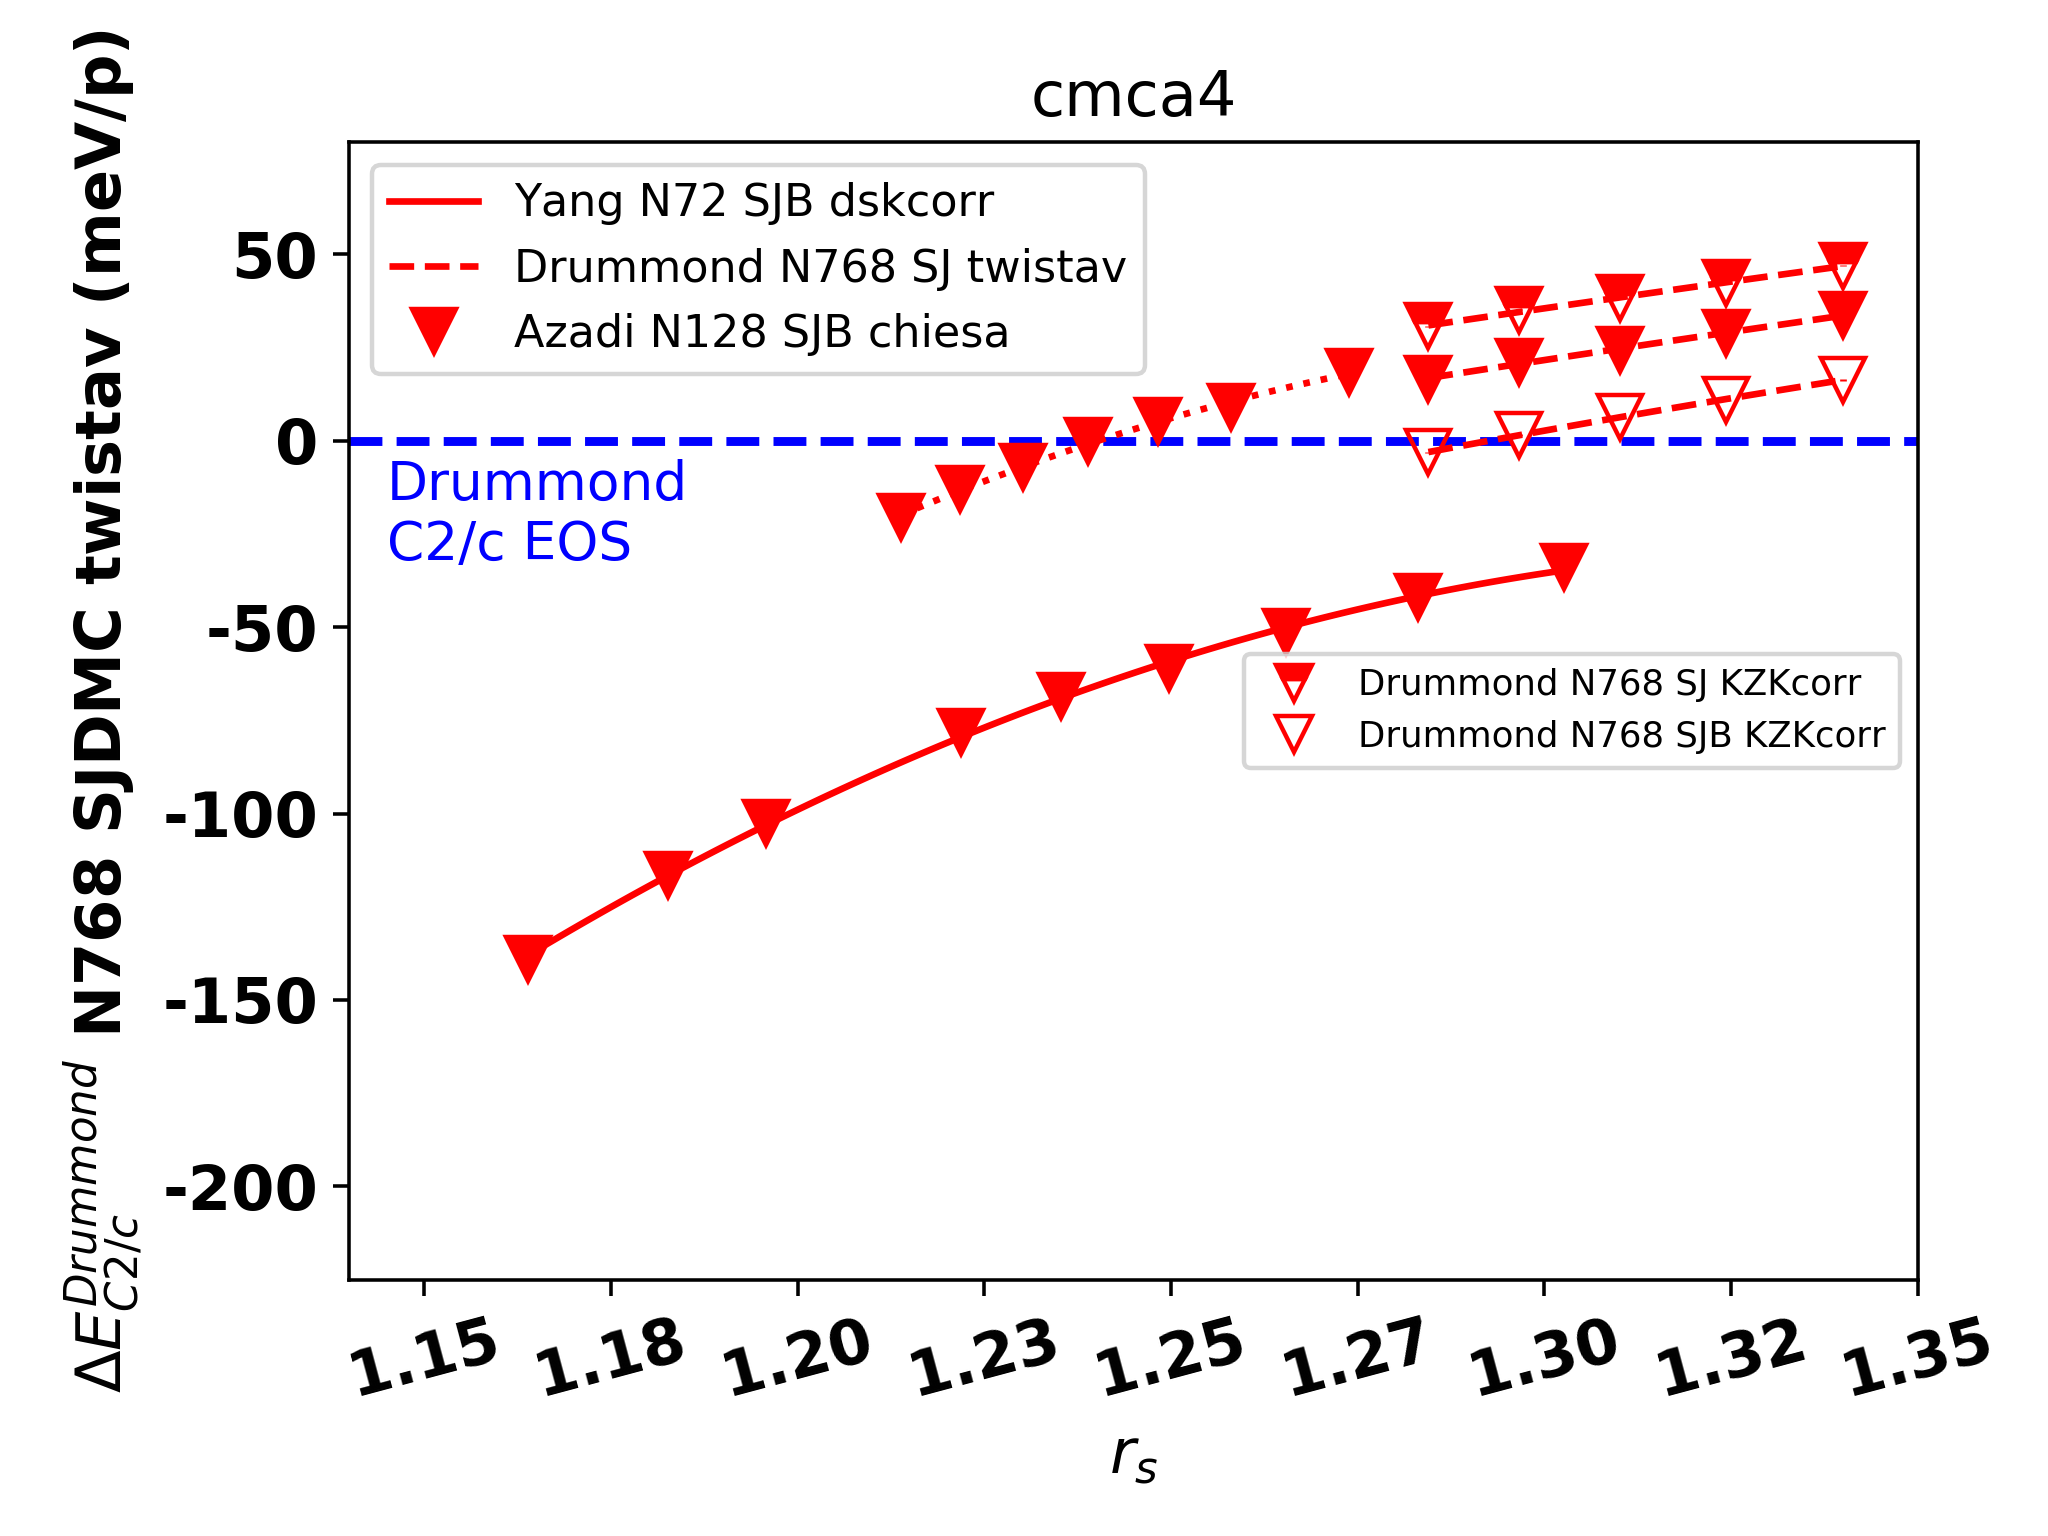
\includegraphics[scale=0.48]{006b_cmca4_step2}
(b) Add back flow to Drummond %\label{fig:static-cmca4-yang-drummond-azadi-sjb}
\end{minipage}
\caption{Cmca-4\label{fig:static-cmca4-yang-drummond-azadi}}
\end{figure}

\subsection{Molecular Candidate Cmca-12}

Three sets of data are shown in Fig.~\ref{fig:static-cmca12-yang-drummond-azadi-data}. The right-filled triangles connected by a dashed line near -100 meV/p at low density ($r_s>1.27$) are Drummond's N96 SJ twistav results. The right-filled triangles connected by a dotted line are Azadi's N96 SJB twistav results. The solid triangles connected by a solid line are my N72 SJB dskcorr results. At $r_s=1.30$ my SBJ dskcorr energy is lower than Drummond's SBJ KZKcorr energy by \textbf{41 meV/p}.

In Fig.~\ref{fig:static-cmca12-yang-drummond-azadi-kzk}, Drummond's N768 SJB KZKcorr results are added as open triangles.

Azadi's N96 SJB twistav energies are higher than Drummond's N96 SJ twistav. This is surprising. No FS correction scheme beyond twist averaging is applied to either data set. Both Azadi and Drummond use PBE geometry, so their structures should agree. I expect Azadi's SJB energy to be lower than Drummond's SJ energy due to the inclusion of back flow. However, actual data indicate the contrary.

\begin{figure}[h]
\begin{minipage}{0.48\textwidth}
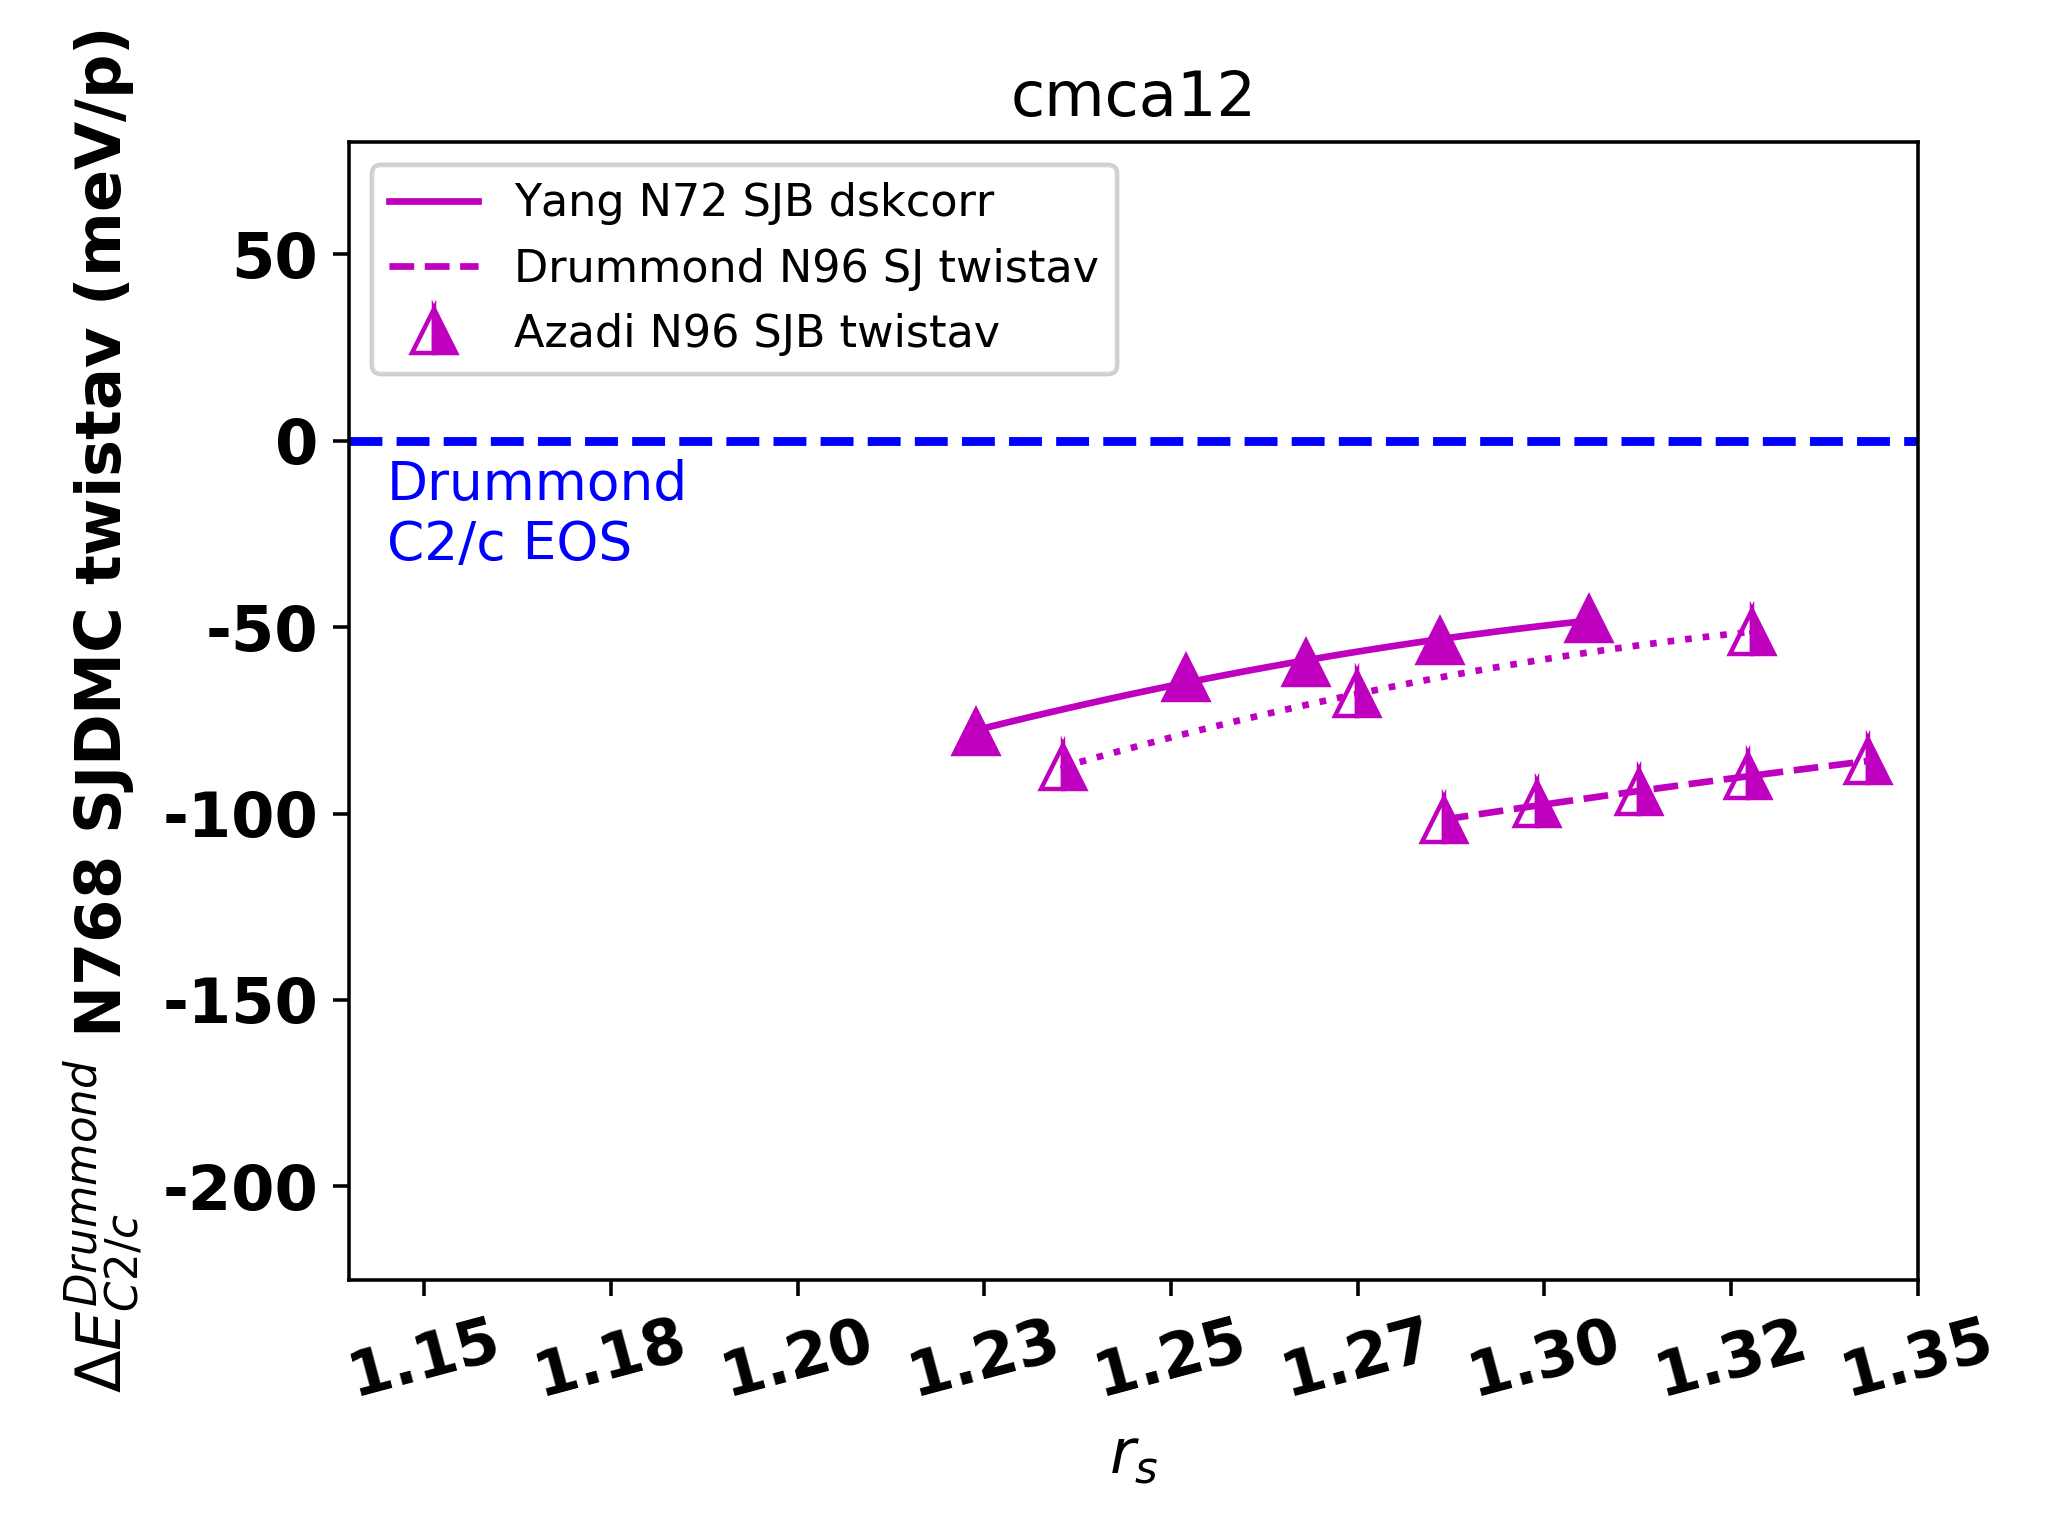
\includegraphics[width=\columnwidth]{006b_cmca12_step0}
%\caption{DMC data.\label{fig:static-cmca12-yang-drummond-azadi-data}}
\end{minipage}
\begin{minipage}{0.48\textwidth}
\includegraphics[width=\columnwidth]{006b_cmca12_step1}
%\caption{DMC data.\label{fig:static-cmca12-yang-drummond-azadi-kzk}}
\end{minipage}
\caption{Cmca-12\label{fig:static-cmca12-yang-drummond-azadi}}
\end{figure}


%\printbibliography[heading=general]
\section{Classical Protons}

Classical protons at zero temperature have no kinetic energy. They serve as a lattice of point Coulomb potential sources and modify the interaction potential of the electron gas. In this case, one simulates the electronic Hamiltonian
\begin{align}
\mathcal{H}_e = -\frac{\hbar^2}{2 m_e}\sum\limits_i^{N_e} \nabla_e^2 + \sum\limits_{i,j,i\neq j}^{N_e+N_p} \frac{e^2q_iq_j}{r_{ij}},
\end{align}
where $e$ denotes electron and $p$ denotes proton. In solid hydrogen, the electronic energy is O(1Ry/p). Candidate structures are separated by energies O(10mha/p) above 300 GPa. At pressures above 300 GPa, the zero-point vibration energy (ZPE) of the protons is 200-400 meV/p O(10 mha/p). The proton ZPE increases with pressure by roughly 40 meV/p for every 100 GPa [Azadi2014SI]. The proton ZPE is large compared to the energy difference among candidate structures and varies significantly with pressure. Therefore, static-proton stimulations cannot reliably predict the transition pressure between candidate structures. Nevertheless, static-proton simulations are crucial as they are often the starting points or building blocks in a dynamic-proton simulation. Further, static calculations are easier to compare than dynamic calculations thanks to fixed protons and crystal symmetries.

In the following, three molecular candidates (C2/c-24, Cmca-4, Cmca-12) and one atomic candidate (I4$_1$/amd) are considered. A lower pressure ($<200$ GPa) molecular candidate (P6$_1$22-36 [Monserrat2016]) is ignored. For each candidate, I start by presenting all available DMC data with no interpretation. I then interpret the difference among different data sets.

\subsection{Phase III candidate C2/c-24}

Three sets of DMC data are presented in Fig.~\ref{fig:static-c2c-yang-drummond}. A series of calculations are added in Fig.~\ref{fig:static-c2c-yang-drummond-data}-\ref{fig:static-c2c-yang-drummond-last} to connect them. In Fig.~\ref{fig:static-c2c-yang-drummond-data}, the total energy reference (in units of ha/p) is
\begin{align}
E(\nu) = \frac{2.140201}{\nu^2} + \frac{0.605212}{\nu} - 0.607313, \label{eq:drum_sjdmc_n768}
\end{align}
where $\nu=\frac{4}{3}\pi r_s^3$ is volume per electron in units of bohr$^3$. The EOS in eq.~\ref{eq:drum_sjdmc_n768} is fitted using all data from the Drummond SJ N768 twistav data set. Three calculations at the highest density from this reference data set are shown as filled diamonds near $\Delta E=0$. The reference data are not exact at zero because the EOS fit is not perfect. However, the error of the EOS fit can be neglected at the scale of the plot O(100 meV/p). The right-filled diamonds are N96 SJ calculations from Drummond. No FS correction beyond twist averaging is applied to these 96-atom results. Finally, the filled diamonds connected by a solid line are my calculations Yang SJB N72 dskcorr. Drummond used PBE structures, whereas Yang used vdW-DF geometries. H$_2$ bond length in PBE structures is roughly 6\% higher than that in vdW structures.

In Fig.~\ref{fig:static-c2c-yang-drummond-repro}, I reproduce Drummond SJ N96 twistav using QMCPACK (open circle). In Fig.~\ref{fig:static-c2c-yang-drummond-fs}, I apply dskcorr to this simulation (upward open triangle) and find the energy to be 7.5 meV/p lower than Drummond's N768 SJ twistav result. In Fig.~\ref{fig:static-c2c-yang-drummond-bf}, I add back flow transformation to the previous simulation and find the energy to decrease by 33 meV before dskcorr (not shown) and 35 meV/p after dskcorr (downward open triangle). In Fig.~\ref{fig:static-c2c-yang-drummond-geo}, I rerun my vdw-DF geometry using 96 protons and reproduce the 72-proton energy within 4(1) meV/p after dskcorr (open square). In Fig.~\ref{fig:static-c2c-yang-drummond-last}, Drummond's back flow results are added as disconnected open diamonds. They are 16 meV/p below the N768 SJ results independent of density. However, Drummond's back flow results include the KZKcorr=13-14 meV/p, so the actual energy gain due to back flow correlation is $\sim$ 30 meV/p [Drummond2016SI]. At $r_s\approx1.30$ my SBJ dskcorr energy is lower than Drummond's SJB KZKcorr energy by \textbf{39 meV/p}.

To estimate energy gained by using vdW-DF geometry instead of PBE geometry. We first observe that the open downward triangle (PBE-geo N96 SJB) is 12 meV/p above the solid line connecting my vdW-geo N72 SJB results. The open square (vdW-geo N96 SJB) is 4 meV/p above the filled diamond it is supposed to reproduce. If this difference 4 meV/p is taken to be the residual FS error after dskcorr, then the vdW geometry lowers DMC energy by 8 meV/p from PBE geometry. 

To estimate remaining FS error after the dskcorr correction, I first assume Drummond N768 KZKcorr results to be the correct thermodynamic values within 1 meV/p. My PBE-geo N72 SJ dskcorr energy is 7.5 meV/p lower than Drummond's N768 SJ twistav energy, which is in turn 13-14 meV/p lower than the KZKcorr result. Thus, I estimate the remaining FS error to be 21 meV/p for the SJ WF. My N72 SJB dskcorr energy is 39 meV/p lower than Drummond's N768 SJB KZKcorr energy. Removing the 8 meV/p gained by vdW geometry, I estimate the remaining FS correction to be 31 meV/p for the SJB WF.

From the above data, I conclude that my data differ from Drummond's in geometry ($\sim$8 meV/p) and FS (21 meV/p for SJ and 31 meV/p for SJB). The SJ FS error is likely the sub-leading order kinetic corrections due to a lack of long-range Jastrow which are not captured by the mixed-estimator S(k). The SJB FS error is likely backflow kinetic corrections. Both vdW-DF geometry and FS make my energies lower. The additional FS error should be corrected.

\begin{figure}[h]
\begin{minipage}{0.48\textwidth}
\includegraphics[scale=0.48]{006b_c2c_step0}
(a) DMC data.%\label{fig:static-c2c-yang-drummond-data}
\end{minipage}
%\begin{subfigure}{0.48\textwidth}
%\includegraphics[scale=0.48]{figures/c2c/006b_c2c_step2}
%\caption{Reproduce PBE-geo N768 SJ twistav.\label{fig:static-c2c-yang-drummond-fs}}
%\end{subfigure}
%\begin{subfigure}{0.48\textwidth}
%\includegraphics[scale=0.48]{figures/c2c/006b_c2c_step3}
%\caption{Effect of backflow.\label{fig:static-c2c-yang-drummond-bf}}
%\end{subfigure}
%\begin{subfigure}{0.48\textwidth}
%\includegraphics[scale=0.48]{figures/c2c/006b_c2c_step4}
%\caption{Effect of vdW-geo.\label{fig:static-c2c-yang-drummond-geo}}
%\end{subfigure}
\begin{minipage}{0.48\textwidth}
\includegraphics[scale=0.48]{006b_c2c_step5}
(b) Drummond SJB. %\label{fig:static-c2c-yang-drummond-last}
\end{minipage}
\caption{C2/c-24 DMC total energy relative to reference EOS.\label{fig:static-c2c-yang-drummond}}
\end{figure}

\subsection{Atomic Phase Candidate I4$_1$/amd}

Four sets of data are shown in Fig.~\ref{fig:static-i41amd-yang-mcminis-azadi}. A series of calculations are added in Fig.~\ref{fig:static-i41amd-yang-mcminis-azadi-data}-\ref{fig:static-i41amd-yang-mcminis-azadi-last} to connect them. Phase III EOS eqn.~\ref{eq:drum_sjdmc_n768} is again used as reference. The solid stars connected by a dot-dashed line are McMinis' SJ results. The solid stars connected by a dotted line are Azadi's FS-corrected results. The solid stars connected by a solid line are my results. Finally, the right-filled starts connected by dot-dashed lines are Azadi's N128 SJB twistav results without the Chiesa correction.

In Fig.~\ref{fig:static-i41amd-yang-mcminis-azadi-repro}, I attempt to reproduce Azadi's 128-atom results using QMCPACK (open stars). At $r_s=1.25$, our energies agree within 3 sigmas. However, at $r_s=1.17$, my energy is 18 meV/p higher than Azadi's. In Fig.~\ref{fig:static-i41amd-yang-mcminis-azadi-fs}, I add dskcorr to previous simulations and reproduce my N72 SJB energies (open downward triangles). In Fig.~\ref{fig:static-i41amd-yang-mcminis-azadi-last}, I remove back flow from previous simulations and obtain energies close to McMinis' results. At $r_s=1.17$, my N128 SJ dskcorr energy is 8(2) meV/p lower than McMinis'.

The difference between my N72 SJ dskcorr and McMinis' Ninf SJ energy is 8 meV/p. Assuming McMinis' energies are the correct thermodynamic values, then the remaining FS error after dskcorr is 8 meV/p. This is much lower than the remaining FS error in the molecular structures. Further, comparing the upward open triangles (SJ) and the downward open triangles (SJB), we see that back flow transformation gains $\sim$40 meV/p. Indeed, after shifting McMinis' energies by 48 meV/p (1.8 mha/p), our results agree well (Fig.~\ref{fig:static-enthalpy-vs-pressure}).

The 18 meV/p energy difference between mine and Azadi's twistav energies cannot be satisfactorily explained. Azadi used a different atomic structures than McMinis and myself. However, the energy variation caused by the structure difference should be no more than 5 meV/p.

%\begin{figure}[h]
%\begin{subfigure}{0.48\textwidth}
%\includegraphics[scale=0.48]{figures/i41amd/006b_i41amd_step0}
%\caption{DMC data.\label{fig:static-i41amd-yang-mcminis-azadi-data}}
%\end{subfigure}
%\begin{subfigure}{0.48\textwidth}
%\includegraphics[scale=0.48]{figures/i41amd/006b_i41amd_step1}
%\caption{Reproduce PBE-geo N128 SJB twistav.\label{fig:static-i41amd-yang-mcminis-azadi-repro}}
%\end{subfigure}
%\begin{subfigure}{0.48\textwidth}
%\includegraphics[scale=0.48]{figures/i41amd/006b_i41amd_step2}
%\caption{Match N96 and N72 using dskcorr.\label{fig:static-i41amd-yang-mcminis-azadi-fs}}
%\end{subfigure}
%\begin{subfigure}{0.48\textwidth}
%\includegraphics[scale=0.48]{figures/i41amd/006b_i41amd_step3}
%\caption{Reproduce McMinis SJ.\label{fig:static-i41amd-yang-mcminis-azadi-last}}
%\end{subfigure}
%\caption{I4$_1$/amd\label{fig:static-i41amd-yang-mcminis-azadi}}
%\end{figure}

\subsection{Molecular Candidate Cmca-4}

Three sets of data are shown in Fig.~\ref{fig:static-cmca4-yang-drummond-azadi}. The same reference EOS eq.~(\ref{eq:drum_sjdmc_n768}) is used as before. The solid downward triangles connected by a dashed line are Drummond N768 SJ twistav results. The solid downward triangles connected by a dotted line are Azadi's N128 SJB chiesa results [Azadi2014SI]. Finally, the solid downward triangles connected by a solid line are my N72 SJB dskcorr results.

In Fig.~\ref{fig:static-cmca4-yang-drummond-azadi-kzk}, KZKcorr=13-14 meV/p is added to Drummond SJ results to produce the top-filled downward triangles. In Fig.~\ref{fig:static-cmca4-yang-drummond-azadi-sjb}, Drummond's back flow results, corrected by KZKcorr, are shown as open downward triangles. At $r_s=1.30$ my SBJ dskcorr energy is lower than Drummond's SBJ KZKcorr energy by \textbf{37 meV/p}.

Azadi's SJB results are more consistent with Drummond's SJ results than SJB results. This discrepancy is unlikely to be due to the Chiesa correction because the remaining FS error after the Chiesa correction is usually negative.

\begin{figure}[h]
\begin{minipage}{0.48\textwidth}
\includegraphics[width=\columnwidth]{006b_cmca4_step0}
 (a) DMC data.%\label{fig:static-cmca4-yang-drummond-azadi-data}
\end{minipage}
%\begin{subfigure}{0.48\textwidth}
%\includegraphics[scale=0.48]{figures/cmca4/006b_cmca4_step1}
%\caption{Add KZKcorr to Drummond.\label{fig:static-cmca4-yang-drummond-azadi-kzk}}
%\end{subfigure}
\begin{minipage}{0.48\textwidth}
\includegraphics[scale=0.48]{006b_cmca4_step2}
(b) Add back flow to Drummond %\label{fig:static-cmca4-yang-drummond-azadi-sjb}
\end{minipage}
\caption{Cmca-4\label{fig:static-cmca4-yang-drummond-azadi}}
\end{figure}

\subsection{Molecular Candidate Cmca-12}

Three sets of data are shown in Fig.~\ref{fig:static-cmca12-yang-drummond-azadi-data}. The right-filled triangles connected by a dashed line near -100 meV/p at low density ($r_s>1.27$) are Drummond's N96 SJ twistav results. The right-filled triangles connected by a dotted line are Azadi's N96 SJB twistav results. The solid triangles connected by a solid line are my N72 SJB dskcorr results. At $r_s=1.30$ my SBJ dskcorr energy is lower than Drummond's SBJ KZKcorr energy by \textbf{41 meV/p}.

In Fig.~\ref{fig:static-cmca12-yang-drummond-azadi-kzk}, Drummond's N768 SJB KZKcorr results are added as open triangles.

Azadi's N96 SJB twistav energies are higher than Drummond's N96 SJ twistav. This is surprising. No FS correction scheme beyond twist averaging is applied to either data set. Both Azadi and Drummond use PBE geometry, so their structures should agree. I expect Azadi's SJB energy to be lower than Drummond's SJ energy due to the inclusion of back flow. However, actual data indicate the contrary.

\begin{figure}[h]
\begin{minipage}{0.48\textwidth}
\includegraphics[width=\columnwidth]{006b_cmca12_step0}
%\caption{DMC data.\label{fig:static-cmca12-yang-drummond-azadi-data}}
\end{minipage}
\begin{minipage}{0.48\textwidth}
\includegraphics[width=\columnwidth]{006b_cmca12_step1}
%\caption{DMC data.\label{fig:static-cmca12-yang-drummond-azadi-kzk}}
\end{minipage}
\caption{Cmca-12\label{fig:static-cmca12-yang-drummond-azadi}}
\end{figure}


%\chapter{Effect of ions on the electronic momentum distribution}
This chapter is based on the following article(s):

\textit{I}. Yubo Yang, Nozomu Hiraoka, Kazuhiro Matsuda, Markus Holzmann, and David Ceperley, "Quantum Monte Carlo Compton profiles of solid and liquid lithium," arXiv: 1912.12295

\section{Introduction} \label{sec:intro}

The Compton profile is a bulk-sensitive probe of the electronic structure of a material accessible to both theory and experiment. Using the ``impulse approximation''~\cite{Eisenberger1970}, the double differential cross section of inelastic light scattering is directly proportional to the Compton profile, the Radon transform of the electronic momentum distribution along the scattering vector. \begin{equation}
J(p_z) = \iint dk_x dk_y ~ n(k_x, k_y, k_z=p_z),
\end{equation}
where $n(\bs{k})$ is the electronic momentum distribution.
Since the pioneering work of Eisenberger et al.~\cite{Eisenberger1970,Eisenberger1972}, Compton scattering experiments have been performed on simple metals such as Li~\cite{Sakurai1995, Schulke1996,Chen1999,Sternemann2001,Tanaka2001}, Be~\cite{Hamalainen1996,Huotari2000}, Na~\cite{Huotari2010} as well as more complicated materials. Accompanying the scattering experiments are numerous theoretical calculations using different electronic structure theories including density functional theory (DFT)~\cite{Sakurai1995,Schulke1996,Tanaka2001,Jarlborg1998,Baruah1999,Bross2005,Makkonen2005,Klevak2016,Sekania2018}, QMC~\cite{Filippi1999,Huotari2010}, and GW~\cite{Yasunori1997,Schulke1999,Eguiluz2000,Olevano2012}.
The Compton profiles in ref.~\cite{Sakurai1995,Schulke1996} were compared to DFT results using the local density approximation (LDA) with the Lam-Platzman correlation correction~\cite{Lam1974}.
While the Lam-Platzman correction has been shown to be accurate by QMC~\cite{Filippi1999,Schulke2001,Bross2005}, the theoretical Compton profile is still larger at low momenta and smaller at high momenta compared with experiment. In other words, the predicted Compton profile is typically narrower than observed.

Both theoretical approximations and experimental procedures may be responsible for a significant fraction of the aforementioned discrepancy. In the experiment, finite momentum resolution and final-state effects~\cite{Sternemann2000,Soininen2001} broaden the measured Compton profile. In the theoretical calculations, the lack of electronic correlation and the use of pseudopotentials both narrow the computed Compton profile. Furthermore, many subtle complications may also be responsible for part of the discrepancy. Examples include: multiple scattering corrections, background subtraction, thermal expansion, electron-phonon coupling, and relativistic effects.

In this paper, we present much improved QMC calculations on the solid and liquid states of lithium. Firstly, we use grand-canonical twist-averaging~\cite{Lin2001,Holzmann2016} to access the momentum distribution at arbitrary momentum while preserving a sharp Fermi surface. We obtain a momentum resolution of 0.040 a.u., which is higher than the 0.068 a.u. achieved previously~\cite{Filippi1999} (It is straight-forward to further increase momentum resolution given more computational resources). Secondly, we perform diffusion Monte Carlo (DMC) to remove effects of the trial wavefunction. Thirdly, we use all-electron QMC to explore the pseudopotential bias in the Compton profile. We find that the pseudopotential bias is responsible for the majority of discrepancy between pseudopotential QMC and experimental Compton profiles away from the Fermi surface. Fourth and finally, we apply finite-size corrections~\cite{Holzmann2009,Holzmann2011} to obtain the momentum distribution in the thermodynamic limit. Using these improved procedures, we calculate the disorder-averaged Compton profiles for polycrystal and liquid lithium and obtain good agreement with recent high-resolution synchrotron experiment~\cite{Nozomu2019}.

This paper is organized as follows. In section \ref{sec:method}, we describe the simulation methods used to obtain the QMC momentum distributions. In section \ref{sec:results}, we show the QMC momentum distributions and the resulting Compton profiles in comparison with experiment. In section \ref{sec:discussion}, we discuss the influence of various physical effects on the momentum distribution in an attempt to explain the remaining discrepancy between QMC and experiment.

\section{Method} \label{sec:method}

Full-core and pseudopotential QMC calculations have been performed on both  the perfect crystal and disordered lithium configurations. We use Slater-Jastrow trial wavefunction
\begin{equation}
\Psi_T = D^{\up} D^{\dn} \exp\left[ -\sum\limits_{i<j}^{N} u(\bs{r}_i-\bs{r}_j) - \sum\limits_{i=1}^N \chi(\bs{r}_i) \right],\label{eq:sj}
\end{equation}
where $u(\bs{r})$ is the electron-electron Jastrow pair function, $\chi(\bs{r})$ is the electron-ion Jastrow pair function and $\bs{r}_i$ is the position of the i$^{th}$ electron. The Slater determinant $D^{\up/\dn}$ is composed of single-particle orbitals obtained using Kohn-Sham (KS) DFT with the LDA functional. In the full-core calculation, we remove the approximate electron-ion cusp from the orbitals and re-introduce the exact cusp condition in the Jastrow function~\cite{Ceperley1981}. The electron-ion Jastrow pair function is split into a sum of core and valence pieces. A flexible Bspline with 16 adjustable knots is used for the core piece ($r<2$ bohr). An electron-electron-ion three-body Jastrow is also added to further improve the all-electron wavefunction. In the pseudopotential calculation, we treat the lithium atoms as pseudo ions of charge +1. The core, screened by 1s electrons, is replaced by the BFD pseudopotential~\cite{Burkatzki2007}.  The electron-electron Jastrow pair function is expressed as a sum of real-space and reciprocal-space parts to accurately describe long-range plasmon fluctuations.

In variational Monte Carlo (VMC), we sample $\vert \psi_T \vert^2$ using Metropolis Monte Carlo and directly calculate properties from the many-body wavefunction. The momentum distribution is calculated using the direct estimator in reciprocal space\cite{McMillan1965}. In DMC, an ensemble of electron configurations evolve according to the Green's function of the non-relativistic Schr\"odinger equation in imaginary time. Using the trial wavefunction $\psi_T$ as guiding function and phase reference, the long-time solution samples the mixed distribution $\psi^*_T\psi_{FP}$, in the limit of small time step. $\psi_{FP}$ is the fixed-phase ground-state wavefunction. If the phase of $\psi_T$ were exact, then $\psi_{FP}$ would be the exact ground-state wavefunction.~\cite{Ortiz1993} The difference between the expectation value of an observable in the fixed-phase and the mixed distributions is the mixed-estimator bias. We gauge simulation quality by monitoring kinetic, potential, and total energies as well as pair correlation functions and the momentum distribution. We observe fast equilibration, small variance and small mixed-estimator bias in all monitored quantities. The DMC momentum distribution is linearly extrapolated to remove the mixed-estimator bias. For more details on the computational methods and data processing, see the supplementary materials.

We use GCTABC to improve the momentum distribution \cite{PhysRevLett.97.076404,Holzmann2009}. A previous QMC calculation~\cite{Filippi1999} used real wavefunctions and canonical twist average boundary condition (CTABC); each boundary condition (twist) had the same number of electrons. Use of real trial functions restricted the accessible momenta to those commensurate with the simulation cell. CTABC can occupy states outside of the Fermi surface at certain twists, which artificially smears the Fermi surface. In contrast, the grand-canonical twist average technique enforces constant chemical potential at all twists. We adjust the number of electrons at each twist such that no state outside the Fermi surface is occupied. This allows us to sample the momentum distribution at momenta arbitrarily close to the Fermi surface while maintaining a sharp Fermi surface. In practice, we impose the occupation of the orbitals in the Slater determinant according to the LDA Fermi energy. In principle, one might modify the Fermi surface by estimating the chemical potential directly within QMC \cite{yang2019electronic}. However, this is much more computationally demanding and is beyond the scope of the current study and not thought to be necessary for lithium.

In the perfect crystal, the full-core simulation contains 54 lithium atoms, while the pseudopotential simulations contain 54 or 432 atoms. We use MD with the modified embedded-atom potential (MEAM)~\cite{Baskes1992} to generate the disordered configurations.
The MD temperatures were elevated to model quantum fluctuations of the nuclei~\cite{Filippi1998}.
We sample the canonical distribution with 432 lithium atoms at 330K and 500K for experiments at 298K and 493K, respectively.

All calculations have been performed at the same density $r_s=3.25$, consistent with the previous QMC study~\cite{Filippi1999}. After obtaining QMC results at $r_s=3.25$, we rescale the density of QMC Compton profiles to match the experimental densities: $r_s=3.31$ for the liquid and $r_s=3.265$ for the solid.

In both QMC and experiment, we assume the momentum distribution of the core electrons to remain unmodified from that in the isolated atom. The atomic core orbital is calculated using Hartree-Fock (HF) and removed from all-electron results to produce valence electron contributions.

We convolved our QMC Compton profile with a broadening function to model instrument resolution and final-state interaction. For this we used the \emph{extended Lorentzian}
\begin{equation}
b(x) = \frac{1}{\tilde{\Omega}} \frac{1}{
a_0+a_1(\frac{2x}{\Gamma})^2+a_2(\frac{2x}{\Gamma})^4
}\label{eq:elorentz}
\end{equation}
with $\Gamma=0.024$ a.u., $a_0=1$, $a_1=0.85$ and $a_2=0.15$ chosen to fit the convolution of the elastic line in the X-ray experiment and the spectral density function of the electrons and $\tilde{\Omega}$ such that $\int dx ~b(x)=1$. 

We used LAMMPS~\cite{Plimpton1995} for the MD simulations, QE~\cite{Giannozzi2009,Giannozzi2017} for DFT, PySCF~\cite{PYSCF} for HF, and QMCPACK~\cite{Kim2018} for QMC. The disordered calculations have been automated using the nexus suite of tools~\cite{Krogel2016}.

\section{Results} \label{sec:results}

Figure~\ref{fig:sl-jp-djp} shows the valence Compton profiles of solid and liquid lithium from experiment and processed QMC data. The raw QMC data have been processed to account for finite-size effects, thermal disorder, pseudopotential bias, density change, final-state effects, and instrument resolution. The QMC Compton profiles agree with experiment immediately inside the Fermi surface (0.2 a.u.$<$p$<$0.4 a.u.) and at large momenta (p$>$0.9  a.u.). However, the QMC Compton profiles show less high-momentum component immediately outside the Fermi surface and too much low-momentum component. Both the theoretical and experimental valence Compton profiles satisfy the normalization sum rule ($\int_{-\infty}^{\infty} J(p)dp=1$) to better than 0.3\%. The difference between QMC and experiment Compton profiles can be interpreted as a shift of momentum density from zero to slightly above the Fermi momentum. 

\begin{figure}[h]
\includegraphics[width=\linewidth]{li58_sl-jp}
\caption{Valence electronic Compton profiles of solid (solid line) and liquid (dashed line) lithium from QMC (thin) and experiment (thick). The top panel shows the Compton profiles on an absolute scale. The bottom panel shows  $\Delta J(p)=J_{QMC}-J_{expt}$.}\label{fig:sl-jp-djp}
\end{figure}

Figure~\ref{fig:s-l-djp} shows the change of the Compton profile when the liquid freezes into a solid. The systematic difference  between QMC calculations and experiment is almost identical in the solid and liquid. Thus, cancellation of error allows us to capture the difference between the solid and liquid Compton profiles almost perfectly.
The main change is a density-induced outward shift of the Fermi surface. This shift manifests in Fig.~\ref{fig:s-l-djp} as a peak at the solid Fermi momentum $p_F\approx0.578$ a.u. and a parabolic dip centered around $p=0$. Another important difference is the emergence of secondary Fermi surfaces, due to Umklapp scattering in the solid. We expect secondary Fermi surfaces to center around the reciprocal lattice of the lithium crystal. Crystalline lithium is BCC with a lattice constant of $\sim 6.63$ bohr, so its reciprocal lattice is FCC with a lattice constant of $\sim 1.895$ a.u.. The nearest neighbor to $\Gamma$ is $p_1=1.34$ a.u.  along [110]. Therefore, the closest secondary Fermi surface is located at $p_1-p_F=0.762$ a.u., which is exactly where we observe a small peak in Fig.~\ref{fig:s-l-djp}.

\begin{figure}[h]
\includegraphics[width=\linewidth]{li52e_sl-djp}
\caption{Difference between solid and liquid valence electronic Compton profiles.\label{fig:s-l-djp}}
\end{figure}

As mentioned at the beginning of this section, we process the raw QMC data in several steps to make them comparable to experiment. In the following, we present perfect lithium crystal QMC calculations, which we use to validate the processing steps.

In Fig.~\ref{fig:nk}, 1D slices of the QMC valence momentum distributions are shown. The momentum distribution is free-electron-like along the [100] and [111] directions. Along the [110] direction, however, there is a pronounced secondary Fermi surface. The valence profile from the full-core calculation is flatter inside the Fermi surface and has enhanced secondary features when compared to the pseudopotential calculation. 

To obtain the valence momentum distribution from the full-core QMC calculation, we remove the momentum distribution of the 1s core electrons. The 1s orbital of the neutral lithium atom is calculated using Hartree-Fock (HF) with a cc-pV5Z basis. The most pronounced effect of the pseudopotential is to increase the electronic momentum density inside the Fermi surface, raising $n(0)$ by more than 5\%. In contrast, the effect of increasing system size peaks at the Fermi momentum. The main effect of finite system size is to increase the magnitude of the discontinuity at the Fermi momentum. The effects of pseudopotential and finite system size can be better shown in the momentum distribution differences.

\begin{figure}[h]
\begin{minipage}{\columnwidth}
\includegraphics[width=\linewidth]{li57_dmcfc-fcv-dir}
(a) full-core valence \textit{vs} pseudopotential
\end{minipage}
\begin{minipage}{\columnwidth}
\includegraphics[width=\linewidth]{li52g_bfd-crystal-n54-n432-nk}
(b) 432 atoms \textit{vs} 54 atoms
\end{minipage}
\caption{Momentum distribution of valence electrons in lithium BCC crystal. The top panel compares pseudopotential (crosses) to full-core (dots) result.
The bottom panel compares 54-atom (crosses) to 432-atom (pluses) pseudopotential results.\label{fig:nk}}
\end{figure}

In Fig.~\ref{fig:dnk}, we show two sets of momentum distribution differences in direct correspondence with Fig.~\ref{fig:nk}. The first is the difference between full-core and pseudopotential momentum distributions. This difference can be considered a pseudopotential correction (PPC). The PPC is largest inside the Fermi surface. It has a parabolic shape and is mostly negative along the [100] and [111] directions. However, it shows positive peaks near the secondary Fermi surface along the [110] direction.  The PPC is spherically-averaged and applied to the momentum distributions of the disordered structures.

Now consider how the finite size of our supercell affects the results: the finite-size correction (FSC). Figure~\ref{fig:dnk}(b) shows the difference between the 432-atom and 54-atom pseudopotential calculations. The difference peaks at the Fermi surface and goes to zero at high momenta.  The FSC results shown here are used to validate the approach outlined in ref.~\cite{Holzmann2009} and ref.~\cite{Holzmann2011}.

\begin{figure}
\begin{minipage}{\columnwidth}
\includegraphics[width=\linewidth]{li57_dmcfc-ppc-dir}
(a) full-core valence - pseudopotential
\end{minipage}
\begin{minipage}{\columnwidth}
\includegraphics[width=\linewidth]{li52g_bfd-crystal-n54-n432-dnk}
(b) 432 atoms - 54 atoms
\end{minipage}
\caption{Momentum distribution differences. The top panel is the difference between full-core and pseudopotential results. The bottom panel is the difference between the 432-atom and 54-atom pseudopotential results. The shaded region show one standard deviation of statistical uncertainty. These results are used to inform pseudopotential and finite-size corrections. \label{fig:dnk}}
\end{figure}

In Fig.~\ref{fig:crystal-vcp}, we show our best QMC Compton profile in the crystal as the red line. It is the spherically-averaged Compton profile from the 432-atom pseudopotential calculation with PPC and FSC applied. Further, we rescaled the QMC data to change density from $r_s=3.25$ to $r_s=3.265$ and convolved the QMC Compton profile with Eq.~(\ref{eq:elorentz}) to approximately account for experimental resolution and final-state effects. The full-core QMC profiles agrees well with the most recent experiment away from the Fermi surface.

The Compton profile reported by Filippi and Ceperley \cite{Filippi1999} is closer to our full-core than to our pseudopotential result. This is because they accounted for proper core-valence orthogonalization using full-core LDA. Pseudopotential QMC was used to estimate the correlation correction, rather than directly provide the Compton profile.


\begin{figure}
\includegraphics[width=\linewidth]{li62g_crystal-jp}
\caption{Spherical average of the valence Compton profile of lithium BCC crystal at $r_s=3.25$. The red solid line is the best QMC result with all processing steps applied. The red dotted curve is our pseudopotential QMC result. The black curve is experiment on polycrystal lithium. \label{fig:crystal-vcp}}
\end{figure}

Taking our best QMC Compton profiles (thin lines in Fig.~\ref{fig:sl-jp-djp}) as reference, we show the remaining difference between the QMC and the experiment Compton profiles as the black curves in Fig.~\ref{fig:sl-corrections}. We also show the effect of each processing step in the calculation of $J(p)$. Finite-size and convolution corrections both peak at the Fermi momentum and are small at the scale of the remaining discrepancy. The density correction is small in the solid but substantial in the liquid, because QMC calculations have been performed close to the solid density. In both cases, the density correction contracts the Fermi sphere and has little effect above the Fermi momentum. In contrast, the pseudopotential correction nearly vanishes at the Fermi momentum, smoothly transfers low-momentum components to high momenta, and remains non-zero well above the Fermi momentum. The $n(k)$ tail correction is needed to recover the normalization sum rule, because the QMC $n(k)$ is truncated at a finite momentum $k_c$. The exact shape of $n(k)$ tail may not be accurate above $k_c$, because the assumed functional form is simple (see supplemental materials). Fortunately, the effect of $n(k)$ tail within $k_c$ is simply to shift the entire Compton profile up by a constant as dictated by the normalization sum rule. The tail and pseudopotential corrections are the only ones that can change the high-momentum tail of the Compton profile.



\begin{figure}
\includegraphics[width=\linewidth]{li58_solid-the-djp}
\includegraphics[width=\linewidth]{li58_liquid-the-djp}
\caption{Valence Compton profile corrections. The solid black curve is experiment relative to ``best'' theory. The dotted black curve is experiment relative to pseudopotential QMC result with no correction. Each colored curve shows the effect of neglecting a processing step from the theoretical Compton profile. When added to the processed result (solid black curve), the sum of all colored curves approximately recovers the unprocessed result (dotted black curve). \label{fig:sl-corrections}}
\end{figure}

\section{Discussion} \label{sec:discussion}

In the following, we discuss possible explanations for the remaining discrepancy in Fig.~\ref{fig:sl-jp-djp},
which is shown separately for the solid and liquid in Fig.~\ref{fig:sl-corrections}.


{ \bf Electron-Ion interaction} The crystal lattice introduces inhomogeneity to an otherwise homogeneous valence electron density. Umklapp processes send electronic momentum density to secondary Fermi surfaces, thereby enhancing the high-momentum components of the momentum distribution and reducing the momentum distribution inside the Fermi surface. Further, its discontinuity at the Fermi surface is reduced~\cite{Eisenberger1972}.
In the absence of other interactions, the ground-state electronic density will be exact if the electron-ion interaction is perfectly captured. DFT is designed to obtain the correct ground-state electronic density, so we expect it to treat electron-ion interaction well. However, pseudopotential is not designed to faithfully reproduce the charge inhomogeneity of the valence orbital in the core region. Therefore, pseudopotential introduces a bias in the valence momentum distribution.

The qualitative effect of the pseudopotential is clear from its construction. When designing a pseudopotential, one smooths the valence orbital inside the core region. This will decrease the electronic momentum density at high momenta, and increase it at low momenta. Indeed, one can reproduce the pseudopotential correction semi-quantitatively by considering the smoothing of the pseudized valence orbital in the lithium atom (Fig.~\ref{fig:hf-ppc}). We see that augmented planewave (APW) calculations~\cite{Baruah1999,Bross2004,Bross2005,Bross2012} tend to reproduce the experimental Compton profiles better at low momenta than pseudopotential calculations.

\begin{figure}
\includegraphics[width=\linewidth]{li42c_bfd-dmcppc}
\caption{Pseudopotential correction derived from QMC and HF. The green curve is the same QMC pseudopotential correction as shown in Fig.~\ref{fig:sl-corrections}. The dashed blue curve is the pseudopotential correction derived from the all-electron v.s. pseudized lithium atom using HF. The gray vertical line marks the Fermi momentum. \label{fig:hf-ppc}}
\end{figure}

Our pseudopotential correction (PPC) is not perfect. It was derived in the perfect crystal, then applied to the disordered configurations. Ideally, one would directly perform all-electron QMC on the disordered configurations. However, this is computationally expensive. We do not consider all-electron calculation to be necessary in the solid phase, because the effect of disorder is small. The current PPC does over correct the liquid Compton profile at high momenta, because the corrections meant for the secondary Fermi surfaces are extraneous. Nevertheless, we think the pseudopotential bias is mostly captured, i.e. at the scale of Fig.~\ref{fig:hf-ppc}. The corrected Compton profile in Fig.~\ref{fig:crystal-vcp} is in better agreement with experiment than its pseudopotential counterpart, especially at $p=0$. We do not think the pseudopotential bias is responsible for the remaining discrepancy, because the PPC is concentrated around $p=0$. If it were underestimated, then the remaining correction would lower $J(0)$ much more than it would raise $J(p_F)$, worsening the agreement with experiment. 

{\bf Disorder}  Disorder mostly reduces the effect of the crystal lattice, because deviations from the perfect lattice weaken Umklapp processes. A confirmation was obtained when Sternemann et al. reproduced the temperature effect on the Compton profile of lithium by smearing out the pseudopotential with a Debye-Waller factor~\cite{Sternemann2001}.

Thermal disorder is also unlikely to be responsible for the remaining discrepancy because disorder-correction is small at the scale of the remaining correction. This can be seen by comparing the discrepancy in the perfect crystal (Fig.~\ref{fig:crystal-vcp}) to the discrepancy in the disordered solid (Fig.~\ref{fig:sl-jp-djp}). The two remaining discrepancies are similar in both shape and magnitude.



{\bf Electron-Electron Correlation}  The effect of electron-electron (ee) correlation on the momentum distribution is similar to electron-ion interaction in that it increases high-momentum components, decreases low-momentum components and reduces the discontinuity at the Fermi surface. The Slater-Jastrow wavefunction is a first-order modification of the free-electron Slater determinant by the Coulomb interaction~\cite{Holzmann2003} but it does not capture all correlation effects.
However, we expect the Slater-Jastrow wavefunction to be accurate for simple metals. 
Further, it can be systematically improved, for example by using backflow transformations \cite{PhysRevB.91.115106}. 
Calculations on the homogeneous electron gas indicate a small decrease of the discontinuity
at the Fermi 
surface \cite{Holzmann2011} reducing the discrepancy with experiment. Quantitative studies of
backflow effects on the lithium Compton profiles should be addressed in the future.







{\bf Fermi surface}  The Fermi surface of BCC lithium is anisotropic with pronounced secondary features. The DFT Fermi surface is used in the QMC simulation to determine which momentum states to occupy.
For solid lithium, the Fermi surface is nearly spherical. Our DFT Fermi surface of the BCC crystal has a maximum anisotropy of $\delta=5.0\%$, where
\begin{equation} \label{eq:ani-delta}
\delta \equiv \dfrac{k_F^{[110]} - k_F^{[100]}}{k_F^{HEG}}.
\end{equation}
This is in good agreement with the de Haas-van Alphen experiment performed by M. B. Hunt et al.~\cite{Hunt1989}, which reported a maximum anisotropy of $\delta=4.8\pm 0.3\%$. Our DFT result differs from previous calculations by A. H. MacDonald $\delta=3.3\%$~\cite{MacDonald1980} and H. Bross $\delta=5.9\%$~\cite{Bross2005}, likely due to differences in the density functional and pseudopotential.
While the DFT Fermi surface may not be accurate in the crystal,  a liquid is isotropic and will have a spherical Fermi surface.
Given that our solid - liquid Compton profile difference agrees well with experiment (Fig.~\ref{fig:s-l-djp}), we do not consider Fermi surface shape to be responsible for the remaining discrepancy.

{\bf Electron-phonon interaction} We capture disorder effects due to phonons by averaging over thermal atomic configurations. However, other phonon effects are absent from our QMC simulations because the lithium ions are clamped. Phonons scatter quasi-particles and decrease their life times. Thus, we expect the inclusion of electron-phonon interaction to decrease the magnitude of the discontinuity in the momentum distribution. Calculations of the coupled electron-phonon system within the Einstein or Debye model~\cite{PhysRev.131.993} show that the resulting broadening
at zero temperature is essentially given by the Debye frequency.
The Debye temperature of lithium ($<$400K) is much lower than the Fermi temperature of the electrons, so we expect the remaining electron-phonon coupling (not included
in our QMC calculations) to be limited very close to the Fermi surface in momentum space, rendering the effect invisible at the scale of Fig.~\ref{fig:s-l-djp}.


{\bf Finite size effects}  Finite-size effects (FSE) are more challenging to deal with in a many-body simulation than in an effective one-particle theory such as DFT which is formulated for an infinite lattice. In DFT, a calculation performed in a larger simulation cell simply makes the momentum-space grid denser. In contrast, finite system size increases the magnitude of the discontinuity at the Fermi surface in QMC. This effect was found to decrease slowly with system size in the homogeneous electron gas~\cite{Holzmann2009}. This FSE  was analyzed and understood in the homogeneous electron gas~\cite{Holzmann2009,Holzmann2011}. We adopted the same approach here and found good results. In particular, we corrected the FSE using the leading-order expression
\begin{equation} \label{eq:nk-fsc}
\delta n_{\bs{k}}^{(1)} = \int_{-\pi/L}^{\pi/L} \frac{d^3\bs{q}}{(2\pi)^3} \left[
u_q (1-S_q) - nu_q^2 S_q
\right] (n_{\bs{k}+\bs{q}}-n_{\bs{k}}),
\end{equation}
where $u_q$ and $S_q$ are the Jastrow pair function and the structure factor in reciprocal space, which are assumed to take RPA forms at small $q$ and $n$ is the valence electron density. The corrected $n(k)$ from the 54-atom and 432-atom simulations agree well with each other as shown in Fig.~\ref{fig:liquid-nk-fsc}. Therefore, we think finite-size error has been satisfactorily accounted for, and is not responsible for the remaining discrepancy.

\begin{figure}
\includegraphics[width=\linewidth]{li58h_liquid-fsc}
\caption{Finite-size correction in the liquid phase. Dotted lines are pseudopotential QMC $n(k)$ with no correction. Color encodes the number of lithium atoms in the simulation cell. The solid lines correspond to the dotted lines in color and have been corrected using the leading-order expression Eq.~(\ref{eq:nk-fsc}). \label{fig:liquid-nk-fsc}}
\end{figure}

{\bf Density change} The electronic density is a crucial parameter since it determines the Fermi surface. It can change due to thermal expansion and phase transition from solid to liquid.
We accounted for density change between our calculations and experiment by rescaling our computed momentum distributions to the experimental densities by scaling the value of $k$ to match the Fermi momentum ($k_F=(9\pi/4)^{1/3}/r_s$) and then correcting the overall normalization.
This brought the Compton profile into excellent agreement with experiment as shown in Fig.~\ref{fig:s-l-djp}.  Of course it would be possible to perform additional QMC simulations at the experimental density. 

{\bf Final state effects} Finally, the ``impulse approximation'' is known to be inaccurate for core electrons and cause asymmetry in the measured Compton profile~\cite{Eisenberger1970,Sternemann2000,Huotari2001}. To go beyond the ``impulse approximation'', one must consider interaction of the scattered electron with the rest of the system in the final state. Final-state effects are often attributed to three physical interactions. The first is the interaction between the excited quasi-particle with its surrounding medium (self-energy). The second is the interaction between the excited quasi-particle and the hole it lefts behind (vertex correction). The third is the interaction between the hole and a plasmon (plasmaron). C. Sternemann et al. showed that the self-energy combined with the vertex correction can satisfactorily explain the asymmetry of the Compton profile~\cite{Sternemann2000}. The effect of final-state interaction on the Compton profile can be approximated by convolving the spectral density function (SDF) of the excited electron with the ground-state Compton profile~\cite{Soininen2001}. This convolution smears out the derivative-discontinuity of the Compton profile at the Fermi momentum. Thus the convolution correction also peaks at the Fermi momentum.

We account for final-state effects by convolving the QMC Compton profiles with the broadening function Eq.~(\ref{eq:elorentz}), which is an accurate representation of the convolution of the experimental resolution function and the SDF obtained by Soininen et al.~\cite{Soininen2001}. However, the SDF in ref.~\cite{Soininen2001} did not include plasmaron or electron-hole effects. Further, we find near perfect agreement with experiment if the QMC profiles were broadened using a Lorentzian having FWHM $\Gamma=0.026$. In other words, if the neglected final-state effects were to introduce long tails into the SDF, then the QMC profiles would agree much better with experiment. Therefore, final-state effect is a plausible explanation for much of the remaining discrepancy.

\section{Conclusion and Outlook}

Leveraging new algorithms and hardware, we improved the QMC Compton profile of lithium and provided the first QMC results in the disordered solid and the liquid states. Our QMC Compton profiles agree very well with the most recent synchrotron experiment~\cite{Nozomu2019}. We resolved the discrepancy between pseudopotential QMC and experiment at zero and high momenta using an all-electron QMC calculation. We discussed potential explanations for the remaining discrepancy, which is concentrated at the Fermi surface. Future studies should consider final-state effects.

Current state-of-the-art QMC algorithms are ready to aid synchrotron experiments in understanding the measured Compton profiles. It would be interesting to revisit the challenging problem that is the 3D reconstructing of the momentum distribution from directional Compton profiles~\cite{Schulke1996,Tanaka2001}. Momentum resolution has been increased by new techniques in both theory and experiment. Further, all-electron QMC for lithium is feasible for perfect crystals in supercells containing thousands of electrons. The comparison between lithium and sodium will be particularly interesting, because they have the same crystal structure but very different electron-ion interactions~\cite{Eisenberger1972}. A detailed study of these systems can shed more light on the nature of electron-ion and perhaps the electron-phonon interactions in simple metals.

Finally, when sufficient accuracy has been achieved in both theory and experiment, one can study the difference between ground-state (QMC) and final-state (experimental) Compton profiles to extract information on the dynamic structure factor of the system.


%\printbibliography{[heading=general]}
\section{Introduction} \label{sec:intro}

The Compton profile is a bulk-sensitive probe of the electronic structure of a material accessible to both theory and experiment. Using the ``impulse approximation''~\cite{Eisenberger1970}, the double differential cross section of inelastic light scattering is directly proportional to the Compton profile, the Radon transform of the electronic momentum distribution along the scattering vector. \begin{equation}
J(p_z) = \iint dk_x dk_y ~ n(k_x, k_y, k_z=p_z),
\end{equation}
where $n(\bs{k})$ is the electronic momentum distribution.
Since the pioneering work of Eisenberger et al.~\cite{Eisenberger1970,Eisenberger1972}, Compton scattering experiments have been performed on simple metals such as Li~\cite{Sakurai1995, Schulke1996,Chen1999,Sternemann2001,Tanaka2001}, Be~\cite{Hamalainen1996,Huotari2000}, Na~\cite{Huotari2010} as well as more complicated materials. Accompanying the scattering experiments are numerous theoretical calculations using different electronic structure theories including density functional theory (DFT)~\cite{Sakurai1995,Schulke1996,Tanaka2001,Jarlborg1998,Baruah1999,Bross2005,Makkonen2005,Klevak2016,Sekania2018}, QMC~\cite{Filippi1999,Huotari2010}, and GW~\cite{Yasunori1997,Schulke1999,Eguiluz2000,Olevano2012}.
The Compton profiles in ref.~\cite{Sakurai1995,Schulke1996} were compared to DFT results using the local density approximation (LDA) with the Lam-Platzman correlation correction~\cite{Lam1974}.
While the Lam-Platzman correction has been shown to be accurate by QMC~\cite{Filippi1999,Schulke2001,Bross2005}, the theoretical Compton profile is still larger at low momenta and smaller at high momenta compared with experiment. In other words, the predicted Compton profile is typically narrower than observed.

Both theoretical approximations and experimental procedures may be responsible for a significant fraction of the aforementioned discrepancy. In the experiment, finite momentum resolution and final-state effects~\cite{Sternemann2000,Soininen2001} broaden the measured Compton profile. In the theoretical calculations, the lack of electronic correlation and the use of pseudopotentials both narrow the computed Compton profile. Furthermore, many subtle complications may also be responsible for part of the discrepancy. Examples include: multiple scattering corrections, background subtraction, thermal expansion, electron-phonon coupling, and relativistic effects.

In this paper, we present much improved QMC calculations on the solid and liquid states of lithium. Firstly, we use grand-canonical twist-averaging~\cite{Lin2001,Holzmann2016} to access the momentum distribution at arbitrary momentum while preserving a sharp Fermi surface. We obtain a momentum resolution of 0.040 a.u., which is higher than the 0.068 a.u. achieved previously~\cite{Filippi1999} (It is straight-forward to further increase momentum resolution given more computational resources). Secondly, we perform diffusion Monte Carlo (DMC) to remove effects of the trial wavefunction. Thirdly, we use all-electron QMC to explore the pseudopotential bias in the Compton profile. We find that the pseudopotential bias is responsible for the majority of discrepancy between pseudopotential QMC and experimental Compton profiles away from the Fermi surface. Fourth and finally, we apply finite-size corrections~\cite{Holzmann2009,Holzmann2011} to obtain the momentum distribution in the thermodynamic limit. Using these improved procedures, we calculate the disorder-averaged Compton profiles for polycrystal and liquid lithium and obtain good agreement with recent high-resolution synchrotron experiment~\cite{Nozomu2019}.

This paper is organized as follows. In section \ref{sec:method}, we describe the simulation methods used to obtain the QMC momentum distributions. In section \ref{sec:results}, we show the QMC momentum distributions and the resulting Compton profiles in comparison with experiment. In section \ref{sec:discussion}, we discuss the influence of various physical effects on the momentum distribution in an attempt to explain the remaining discrepancy between QMC and experiment.

\section{Method} \label{sec:method}

Full-core and pseudopotential QMC calculations have been performed on both  the perfect crystal and disordered lithium configurations. We use Slater-Jastrow trial wavefunction
\begin{equation}
\Psi_T = D^{\up} D^{\dn} \exp\left[ -\sum\limits_{i<j}^{N} u(\bs{r}_i-\bs{r}_j) - \sum\limits_{i=1}^N \chi(\bs{r}_i) \right],\label{eq:sj}
\end{equation}
where $u(\bs{r})$ is the electron-electron Jastrow pair function, $\chi(\bs{r})$ is the electron-ion Jastrow pair function and $\bs{r}_i$ is the position of the i$^{th}$ electron. The Slater determinant $D^{\up/\dn}$ is composed of single-particle orbitals obtained using Kohn-Sham (KS) DFT with the LDA functional. In the full-core calculation, we remove the approximate electron-ion cusp from the orbitals and re-introduce the exact cusp condition in the Jastrow function~\cite{Ceperley1981}. The electron-ion Jastrow pair function is split into a sum of core and valence pieces. A flexible Bspline with 16 adjustable knots is used for the core piece ($r<2$ bohr). An electron-electron-ion three-body Jastrow is also added to further improve the all-electron wavefunction. In the pseudopotential calculation, we treat the lithium atoms as pseudo ions of charge +1. The core, screened by 1s electrons, is replaced by the BFD pseudopotential~\cite{Burkatzki2007}.  The electron-electron Jastrow pair function is expressed as a sum of real-space and reciprocal-space parts to accurately describe long-range plasmon fluctuations.

In variational Monte Carlo (VMC), we sample $\vert \psi_T \vert^2$ using Metropolis Monte Carlo and directly calculate properties from the many-body wavefunction. The momentum distribution is calculated using the direct estimator in reciprocal space\cite{McMillan1965}. In DMC, an ensemble of electron configurations evolve according to the Green's function of the non-relativistic Schr\"odinger equation in imaginary time. Using the trial wavefunction $\psi_T$ as guiding function and phase reference, the long-time solution samples the mixed distribution $\psi^*_T\psi_{FP}$, in the limit of small time step. $\psi_{FP}$ is the fixed-phase ground-state wavefunction. If the phase of $\psi_T$ were exact, then $\psi_{FP}$ would be the exact ground-state wavefunction.~\cite{Ortiz1993} The difference between the expectation value of an observable in the fixed-phase and the mixed distributions is the mixed-estimator bias. We gauge simulation quality by monitoring kinetic, potential, and total energies as well as pair correlation functions and the momentum distribution. We observe fast equilibration, small variance and small mixed-estimator bias in all monitored quantities. The DMC momentum distribution is linearly extrapolated to remove the mixed-estimator bias. For more details on the computational methods and data processing, see the supplementary materials.

We use GCTABC to improve the momentum distribution \cite{PhysRevLett.97.076404,Holzmann2009}. A previous QMC calculation~\cite{Filippi1999} used real wavefunctions and canonical twist average boundary condition (CTABC); each boundary condition (twist) had the same number of electrons. Use of real trial functions restricted the accessible momenta to those commensurate with the simulation cell. CTABC can occupy states outside of the Fermi surface at certain twists, which artificially smears the Fermi surface. In contrast, the grand-canonical twist average technique enforces constant chemical potential at all twists. We adjust the number of electrons at each twist such that no state outside the Fermi surface is occupied. This allows us to sample the momentum distribution at momenta arbitrarily close to the Fermi surface while maintaining a sharp Fermi surface. In practice, we impose the occupation of the orbitals in the Slater determinant according to the LDA Fermi energy. In principle, one might modify the Fermi surface by estimating the chemical potential directly within QMC \cite{yang2019electronic}. However, this is much more computationally demanding and is beyond the scope of the current study and not thought to be necessary for lithium.

In the perfect crystal, the full-core simulation contains 54 lithium atoms, while the pseudopotential simulations contain 54 or 432 atoms. We use MD with the modified embedded-atom potential (MEAM)~\cite{Baskes1992} to generate the disordered configurations.
The MD temperatures were elevated to model quantum fluctuations of the nuclei~\cite{Filippi1998}.
We sample the canonical distribution with 432 lithium atoms at 330K and 500K for experiments at 298K and 493K, respectively.

All calculations have been performed at the same density $r_s=3.25$, consistent with the previous QMC study~\cite{Filippi1999}. After obtaining QMC results at $r_s=3.25$, we rescale the density of QMC Compton profiles to match the experimental densities: $r_s=3.31$ for the liquid and $r_s=3.265$ for the solid.

In both QMC and experiment, we assume the momentum distribution of the core electrons to remain unmodified from that in the isolated atom. The atomic core orbital is calculated using Hartree-Fock (HF) and removed from all-electron results to produce valence electron contributions.

We convolved our QMC Compton profile with a broadening function to model instrument resolution and final-state interaction. For this we used the \emph{extended Lorentzian}
\begin{equation}
b(x) = \frac{1}{\tilde{\Omega}} \frac{1}{
a_0+a_1(\frac{2x}{\Gamma})^2+a_2(\frac{2x}{\Gamma})^4
}\label{eq:elorentz}
\end{equation}
with $\Gamma=0.024$ a.u., $a_0=1$, $a_1=0.85$ and $a_2=0.15$ chosen to fit the convolution of the elastic line in the X-ray experiment and the spectral density function of the electrons and $\tilde{\Omega}$ such that $\int dx ~b(x)=1$. 

We used LAMMPS~\cite{Plimpton1995} for the MD simulations, QE~\cite{Giannozzi2009,Giannozzi2017} for DFT, PySCF~\cite{PYSCF} for HF, and QMCPACK~\cite{Kim2018} for QMC. The disordered calculations have been automated using the nexus suite of tools~\cite{Krogel2016}.

\section{Results} \label{sec:results}

Figure~\ref{fig:sl-jp-djp} shows the valence Compton profiles of solid and liquid lithium from experiment and processed QMC data. The raw QMC data have been processed to account for finite-size effects, thermal disorder, pseudopotential bias, density change, final-state effects, and instrument resolution. The QMC Compton profiles agree with experiment immediately inside the Fermi surface (0.2 a.u.$<$p$<$0.4 a.u.) and at large momenta (p$>$0.9  a.u.). However, the QMC Compton profiles show less high-momentum component immediately outside the Fermi surface and too much low-momentum component. Both the theoretical and experimental valence Compton profiles satisfy the normalization sum rule ($\int_{-\infty}^{\infty} J(p)dp=1$) to better than 0.3\%. The difference between QMC and experiment Compton profiles can be interpreted as a shift of momentum density from zero to slightly above the Fermi momentum. 

\begin{figure}[h]
\includegraphics[width=\linewidth]{li58_sl-jp}
\caption{Valence electronic Compton profiles of solid (solid line) and liquid (dashed line) lithium from QMC (thin) and experiment (thick). The top panel shows the Compton profiles on an absolute scale. The bottom panel shows  $\Delta J(p)=J_{QMC}-J_{expt}$.}\label{fig:sl-jp-djp}
\end{figure}

Figure~\ref{fig:s-l-djp} shows the change of the Compton profile when the liquid freezes into a solid. The systematic difference  between QMC calculations and experiment is almost identical in the solid and liquid. Thus, cancellation of error allows us to capture the difference between the solid and liquid Compton profiles almost perfectly.
The main change is a density-induced outward shift of the Fermi surface. This shift manifests in Fig.~\ref{fig:s-l-djp} as a peak at the solid Fermi momentum $p_F\approx0.578$ a.u. and a parabolic dip centered around $p=0$. Another important difference is the emergence of secondary Fermi surfaces, due to Umklapp scattering in the solid. We expect secondary Fermi surfaces to center around the reciprocal lattice of the lithium crystal. Crystalline lithium is BCC with a lattice constant of $\sim 6.63$ bohr, so its reciprocal lattice is FCC with a lattice constant of $\sim 1.895$ a.u.. The nearest neighbor to $\Gamma$ is $p_1=1.34$ a.u.  along [110]. Therefore, the closest secondary Fermi surface is located at $p_1-p_F=0.762$ a.u., which is exactly where we observe a small peak in Fig.~\ref{fig:s-l-djp}.

\begin{figure}[h]
\includegraphics[width=\linewidth]{li52e_sl-djp}
\caption{Difference between solid and liquid valence electronic Compton profiles.\label{fig:s-l-djp}}
\end{figure}

As mentioned at the beginning of this section, we process the raw QMC data in several steps to make them comparable to experiment. In the following, we present perfect lithium crystal QMC calculations, which we use to validate the processing steps.

In Fig.~\ref{fig:nk}, 1D slices of the QMC valence momentum distributions are shown. The momentum distribution is free-electron-like along the [100] and [111] directions. Along the [110] direction, however, there is a pronounced secondary Fermi surface. The valence profile from the full-core calculation is flatter inside the Fermi surface and has enhanced secondary features when compared to the pseudopotential calculation. 

To obtain the valence momentum distribution from the full-core QMC calculation, we remove the momentum distribution of the 1s core electrons. The 1s orbital of the neutral lithium atom is calculated using Hartree-Fock (HF) with a cc-pV5Z basis. The most pronounced effect of the pseudopotential is to increase the electronic momentum density inside the Fermi surface, raising $n(0)$ by more than 5\%. In contrast, the effect of increasing system size peaks at the Fermi momentum. The main effect of finite system size is to increase the magnitude of the discontinuity at the Fermi momentum. The effects of pseudopotential and finite system size can be better shown in the momentum distribution differences.

\begin{figure}[h]
\begin{minipage}{\columnwidth}
\includegraphics[width=\linewidth]{li57_dmcfc-fcv-dir}
(a) full-core valence \textit{vs} pseudopotential
\end{minipage}
\begin{minipage}{\columnwidth}
\includegraphics[width=\linewidth]{li52g_bfd-crystal-n54-n432-nk}
(b) 432 atoms \textit{vs} 54 atoms
\end{minipage}
\caption{Momentum distribution of valence electrons in lithium BCC crystal. The top panel compares pseudopotential (crosses) to full-core (dots) result.
The bottom panel compares 54-atom (crosses) to 432-atom (pluses) pseudopotential results.\label{fig:nk}}
\end{figure}

In Fig.~\ref{fig:dnk}, we show two sets of momentum distribution differences in direct correspondence with Fig.~\ref{fig:nk}. The first is the difference between full-core and pseudopotential momentum distributions. This difference can be considered a pseudopotential correction (PPC). The PPC is largest inside the Fermi surface. It has a parabolic shape and is mostly negative along the [100] and [111] directions. However, it shows positive peaks near the secondary Fermi surface along the [110] direction.  The PPC is spherically-averaged and applied to the momentum distributions of the disordered structures.

Now consider how the finite size of our supercell affects the results: the finite-size correction (FSC). Figure~\ref{fig:dnk}(b) shows the difference between the 432-atom and 54-atom pseudopotential calculations. The difference peaks at the Fermi surface and goes to zero at high momenta.  The FSC results shown here are used to validate the approach outlined in ref.~\cite{Holzmann2009} and ref.~\cite{Holzmann2011}.

\begin{figure}
\begin{minipage}{\columnwidth}
\includegraphics[width=\linewidth]{li57_dmcfc-ppc-dir}
(a) full-core valence - pseudopotential
\end{minipage}
\begin{minipage}{\columnwidth}
\includegraphics[width=\linewidth]{li52g_bfd-crystal-n54-n432-dnk}
(b) 432 atoms - 54 atoms
\end{minipage}
\caption{Momentum distribution differences. The top panel is the difference between full-core and pseudopotential results. The bottom panel is the difference between the 432-atom and 54-atom pseudopotential results. The shaded region show one standard deviation of statistical uncertainty. These results are used to inform pseudopotential and finite-size corrections. \label{fig:dnk}}
\end{figure}

In Fig.~\ref{fig:crystal-vcp}, we show our best QMC Compton profile in the crystal as the red line. It is the spherically-averaged Compton profile from the 432-atom pseudopotential calculation with PPC and FSC applied. Further, we rescaled the QMC data to change density from $r_s=3.25$ to $r_s=3.265$ and convolved the QMC Compton profile with Eq.~(\ref{eq:elorentz}) to approximately account for experimental resolution and final-state effects. The full-core QMC profiles agrees well with the most recent experiment away from the Fermi surface.

The Compton profile reported by Filippi and Ceperley \cite{Filippi1999} is closer to our full-core than to our pseudopotential result. This is because they accounted for proper core-valence orthogonalization using full-core LDA. Pseudopotential QMC was used to estimate the correlation correction, rather than directly provide the Compton profile.


\begin{figure}
\includegraphics[width=\linewidth]{li62g_crystal-jp}
\caption{Spherical average of the valence Compton profile of lithium BCC crystal at $r_s=3.25$. The red solid line is the best QMC result with all processing steps applied. The red dotted curve is our pseudopotential QMC result. The black curve is experiment on polycrystal lithium. \label{fig:crystal-vcp}}
\end{figure}

Taking our best QMC Compton profiles (thin lines in Fig.~\ref{fig:sl-jp-djp}) as reference, we show the remaining difference between the QMC and the experiment Compton profiles as the black curves in Fig.~\ref{fig:sl-corrections}. We also show the effect of each processing step in the calculation of $J(p)$. Finite-size and convolution corrections both peak at the Fermi momentum and are small at the scale of the remaining discrepancy. The density correction is small in the solid but substantial in the liquid, because QMC calculations have been performed close to the solid density. In both cases, the density correction contracts the Fermi sphere and has little effect above the Fermi momentum. In contrast, the pseudopotential correction nearly vanishes at the Fermi momentum, smoothly transfers low-momentum components to high momenta, and remains non-zero well above the Fermi momentum. The $n(k)$ tail correction is needed to recover the normalization sum rule, because the QMC $n(k)$ is truncated at a finite momentum $k_c$. The exact shape of $n(k)$ tail may not be accurate above $k_c$, because the assumed functional form is simple (see supplemental materials). Fortunately, the effect of $n(k)$ tail within $k_c$ is simply to shift the entire Compton profile up by a constant as dictated by the normalization sum rule. The tail and pseudopotential corrections are the only ones that can change the high-momentum tail of the Compton profile.



\begin{figure}
\includegraphics[width=\linewidth]{li58_solid-the-djp}
\includegraphics[width=\linewidth]{li58_liquid-the-djp}
\caption{Valence Compton profile corrections. The solid black curve is experiment relative to ``best'' theory. The dotted black curve is experiment relative to pseudopotential QMC result with no correction. Each colored curve shows the effect of neglecting a processing step from the theoretical Compton profile. When added to the processed result (solid black curve), the sum of all colored curves approximately recovers the unprocessed result (dotted black curve). \label{fig:sl-corrections}}
\end{figure}

\section{Discussion} \label{sec:discussion}

In the following, we discuss possible explanations for the remaining discrepancy in Fig.~\ref{fig:sl-jp-djp},
which is shown separately for the solid and liquid in Fig.~\ref{fig:sl-corrections}.


{ \bf Electron-Ion interaction} The crystal lattice introduces inhomogeneity to an otherwise homogeneous valence electron density. Umklapp processes send electronic momentum density to secondary Fermi surfaces, thereby enhancing the high-momentum components of the momentum distribution and reducing the momentum distribution inside the Fermi surface. Further, its discontinuity at the Fermi surface is reduced~\cite{Eisenberger1972}.
In the absence of other interactions, the ground-state electronic density will be exact if the electron-ion interaction is perfectly captured. DFT is designed to obtain the correct ground-state electronic density, so we expect it to treat electron-ion interaction well. However, pseudopotential is not designed to faithfully reproduce the charge inhomogeneity of the valence orbital in the core region. Therefore, pseudopotential introduces a bias in the valence momentum distribution.

The qualitative effect of the pseudopotential is clear from its construction. When designing a pseudopotential, one smooths the valence orbital inside the core region. This will decrease the electronic momentum density at high momenta, and increase it at low momenta. Indeed, one can reproduce the pseudopotential correction semi-quantitatively by considering the smoothing of the pseudized valence orbital in the lithium atom (Fig.~\ref{fig:hf-ppc}). We see that augmented planewave (APW) calculations~\cite{Baruah1999,Bross2004,Bross2005,Bross2012} tend to reproduce the experimental Compton profiles better at low momenta than pseudopotential calculations.

\begin{figure}
\includegraphics[width=\linewidth]{li42c_bfd-dmcppc}
\caption{Pseudopotential correction derived from QMC and HF. The green curve is the same QMC pseudopotential correction as shown in Fig.~\ref{fig:sl-corrections}. The dashed blue curve is the pseudopotential correction derived from the all-electron v.s. pseudized lithium atom using HF. The gray vertical line marks the Fermi momentum. \label{fig:hf-ppc}}
\end{figure}

Our pseudopotential correction (PPC) is not perfect. It was derived in the perfect crystal, then applied to the disordered configurations. Ideally, one would directly perform all-electron QMC on the disordered configurations. However, this is computationally expensive. We do not consider all-electron calculation to be necessary in the solid phase, because the effect of disorder is small. The current PPC does over correct the liquid Compton profile at high momenta, because the corrections meant for the secondary Fermi surfaces are extraneous. Nevertheless, we think the pseudopotential bias is mostly captured, i.e. at the scale of Fig.~\ref{fig:hf-ppc}. The corrected Compton profile in Fig.~\ref{fig:crystal-vcp} is in better agreement with experiment than its pseudopotential counterpart, especially at $p=0$. We do not think the pseudopotential bias is responsible for the remaining discrepancy, because the PPC is concentrated around $p=0$. If it were underestimated, then the remaining correction would lower $J(0)$ much more than it would raise $J(p_F)$, worsening the agreement with experiment. 

{\bf Disorder}  Disorder mostly reduces the effect of the crystal lattice, because deviations from the perfect lattice weaken Umklapp processes. A confirmation was obtained when Sternemann et al. reproduced the temperature effect on the Compton profile of lithium by smearing out the pseudopotential with a Debye-Waller factor~\cite{Sternemann2001}.

Thermal disorder is also unlikely to be responsible for the remaining discrepancy because disorder-correction is small at the scale of the remaining correction. This can be seen by comparing the discrepancy in the perfect crystal (Fig.~\ref{fig:crystal-vcp}) to the discrepancy in the disordered solid (Fig.~\ref{fig:sl-jp-djp}). The two remaining discrepancies are similar in both shape and magnitude.



{\bf Electron-Electron Correlation}  The effect of electron-electron (ee) correlation on the momentum distribution is similar to electron-ion interaction in that it increases high-momentum components, decreases low-momentum components and reduces the discontinuity at the Fermi surface. The Slater-Jastrow wavefunction is a first-order modification of the free-electron Slater determinant by the Coulomb interaction~\cite{Holzmann2003} but it does not capture all correlation effects.
However, we expect the Slater-Jastrow wavefunction to be accurate for simple metals. 
Further, it can be systematically improved, for example by using backflow transformations \cite{PhysRevB.91.115106}. 
Calculations on the homogeneous electron gas indicate a small decrease of the discontinuity
at the Fermi 
surface \cite{Holzmann2011} reducing the discrepancy with experiment. Quantitative studies of
backflow effects on the lithium Compton profiles should be addressed in the future.







{\bf Fermi surface}  The Fermi surface of BCC lithium is anisotropic with pronounced secondary features. The DFT Fermi surface is used in the QMC simulation to determine which momentum states to occupy.
For solid lithium, the Fermi surface is nearly spherical. Our DFT Fermi surface of the BCC crystal has a maximum anisotropy of $\delta=5.0\%$, where
\begin{equation} \label{eq:ani-delta}
\delta \equiv \dfrac{k_F^{[110]} - k_F^{[100]}}{k_F^{HEG}}.
\end{equation}
This is in good agreement with the de Haas-van Alphen experiment performed by M. B. Hunt et al.~\cite{Hunt1989}, which reported a maximum anisotropy of $\delta=4.8\pm 0.3\%$. Our DFT result differs from previous calculations by A. H. MacDonald $\delta=3.3\%$~\cite{MacDonald1980} and H. Bross $\delta=5.9\%$~\cite{Bross2005}, likely due to differences in the density functional and pseudopotential.
While the DFT Fermi surface may not be accurate in the crystal,  a liquid is isotropic and will have a spherical Fermi surface.
Given that our solid - liquid Compton profile difference agrees well with experiment (Fig.~\ref{fig:s-l-djp}), we do not consider Fermi surface shape to be responsible for the remaining discrepancy.

{\bf Electron-phonon interaction} We capture disorder effects due to phonons by averaging over thermal atomic configurations. However, other phonon effects are absent from our QMC simulations because the lithium ions are clamped. Phonons scatter quasi-particles and decrease their life times. Thus, we expect the inclusion of electron-phonon interaction to decrease the magnitude of the discontinuity in the momentum distribution. Calculations of the coupled electron-phonon system within the Einstein or Debye model~\cite{PhysRev.131.993} show that the resulting broadening
at zero temperature is essentially given by the Debye frequency.
The Debye temperature of lithium ($<$400K) is much lower than the Fermi temperature of the electrons, so we expect the remaining electron-phonon coupling (not included
in our QMC calculations) to be limited very close to the Fermi surface in momentum space, rendering the effect invisible at the scale of Fig.~\ref{fig:s-l-djp}.


{\bf Finite size effects}  Finite-size effects (FSE) are more challenging to deal with in a many-body simulation than in an effective one-particle theory such as DFT which is formulated for an infinite lattice. In DFT, a calculation performed in a larger simulation cell simply makes the momentum-space grid denser. In contrast, finite system size increases the magnitude of the discontinuity at the Fermi surface in QMC. This effect was found to decrease slowly with system size in the homogeneous electron gas~\cite{Holzmann2009}. This FSE  was analyzed and understood in the homogeneous electron gas~\cite{Holzmann2009,Holzmann2011}. We adopted the same approach here and found good results. In particular, we corrected the FSE using the leading-order expression
\begin{equation} \label{eq:nk-fsc}
\delta n_{\bs{k}}^{(1)} = \int_{-\pi/L}^{\pi/L} \frac{d^3\bs{q}}{(2\pi)^3} \left[
u_q (1-S_q) - nu_q^2 S_q
\right] (n_{\bs{k}+\bs{q}}-n_{\bs{k}}),
\end{equation}
where $u_q$ and $S_q$ are the Jastrow pair function and the structure factor in reciprocal space, which are assumed to take RPA forms at small $q$ and $n$ is the valence electron density. The corrected $n(k)$ from the 54-atom and 432-atom simulations agree well with each other as shown in Fig.~\ref{fig:liquid-nk-fsc}. Therefore, we think finite-size error has been satisfactorily accounted for, and is not responsible for the remaining discrepancy.

\begin{figure}
\includegraphics[width=\linewidth]{li58h_liquid-fsc}
\caption{Finite-size correction in the liquid phase. Dotted lines are pseudopotential QMC $n(k)$ with no correction. Color encodes the number of lithium atoms in the simulation cell. The solid lines correspond to the dotted lines in color and have been corrected using the leading-order expression Eq.~(\ref{eq:nk-fsc}). \label{fig:liquid-nk-fsc}}
\end{figure}

{\bf Density change} The electronic density is a crucial parameter since it determines the Fermi surface. It can change due to thermal expansion and phase transition from solid to liquid.
We accounted for density change between our calculations and experiment by rescaling our computed momentum distributions to the experimental densities by scaling the value of $k$ to match the Fermi momentum ($k_F=(9\pi/4)^{1/3}/r_s$) and then correcting the overall normalization.
This brought the Compton profile into excellent agreement with experiment as shown in Fig.~\ref{fig:s-l-djp}.  Of course it would be possible to perform additional QMC simulations at the experimental density. 

{\bf Final state effects} Finally, the ``impulse approximation'' is known to be inaccurate for core electrons and cause asymmetry in the measured Compton profile~\cite{Eisenberger1970,Sternemann2000,Huotari2001}. To go beyond the ``impulse approximation'', one must consider interaction of the scattered electron with the rest of the system in the final state. Final-state effects are often attributed to three physical interactions. The first is the interaction between the excited quasi-particle with its surrounding medium (self-energy). The second is the interaction between the excited quasi-particle and the hole it lefts behind (vertex correction). The third is the interaction between the hole and a plasmon (plasmaron). C. Sternemann et al. showed that the self-energy combined with the vertex correction can satisfactorily explain the asymmetry of the Compton profile~\cite{Sternemann2000}. The effect of final-state interaction on the Compton profile can be approximated by convolving the spectral density function (SDF) of the excited electron with the ground-state Compton profile~\cite{Soininen2001}. This convolution smears out the derivative-discontinuity of the Compton profile at the Fermi momentum. Thus the convolution correction also peaks at the Fermi momentum.

We account for final-state effects by convolving the QMC Compton profiles with the broadening function Eq.~(\ref{eq:elorentz}), which is an accurate representation of the convolution of the experimental resolution function and the SDF obtained by Soininen et al.~\cite{Soininen2001}. However, the SDF in ref.~\cite{Soininen2001} did not include plasmaron or electron-hole effects. Further, we find near perfect agreement with experiment if the QMC profiles were broadened using a Lorentzian having FWHM $\Gamma=0.026$. In other words, if the neglected final-state effects were to introduce long tails into the SDF, then the QMC profiles would agree much better with experiment. Therefore, final-state effect is a plausible explanation for much of the remaining discrepancy.

\section{Conclusion and Outlook}

Leveraging new algorithms and hardware, we improved the QMC Compton profile of lithium and provided the first QMC results in the disordered solid and the liquid states. Our QMC Compton profiles agree very well with the most recent synchrotron experiment~\cite{Nozomu2019}. We resolved the discrepancy between pseudopotential QMC and experiment at zero and high momenta using an all-electron QMC calculation. We discussed potential explanations for the remaining discrepancy, which is concentrated at the Fermi surface. Future studies should consider final-state effects.

Current state-of-the-art QMC algorithms are ready to aid synchrotron experiments in understanding the measured Compton profiles. It would be interesting to revisit the challenging problem that is the 3D reconstructing of the momentum distribution from directional Compton profiles~\cite{Schulke1996,Tanaka2001}. Momentum resolution has been increased by new techniques in both theory and experiment. Further, all-electron QMC for lithium is feasible for perfect crystals in supercells containing thousands of electrons. The comparison between lithium and sodium will be particularly interesting, because they have the same crystal structure but very different electron-ion interactions~\cite{Eisenberger1972}. A detailed study of these systems can shed more light on the nature of electron-ion and perhaps the electron-phonon interactions in simple metals.

Finally, when sufficient accuracy has been achieved in both theory and experiment, one can study the difference between ground-state (QMC) and final-state (experimental) Compton profiles to extract information on the dynamic structure factor of the system.


%This chapter is based on the following article(s):

\textit{I}. Yubo Yang, Vitaly Gorelov, Carlo Pierleoni, Markus Holzmann, and David Ceperley, ``Electronic band gaps from quantum Monte Carlo methods," Phys. Rev. B \textbf{101}, 085115 (2020).

\newcommand \beq{\begin{eqnarray}}
\newcommand \eeq{\end{eqnarray}}
\newcommand \bea{\begin{eqnarray}}
\newcommand \eea{\end{eqnarray}}
\newcommand \avec{{\bf a}}
\newcommand \kvec{{\bf k}}
\newcommand \lvec{{\bf l}}
\newcommand \qvec{{\bf q}}
\newcommand \pvec{{\bf p}}
\newcommand \hvec{{\bf h}}
\newcommand \nvec{{\bf n}}
\newcommand \xvec{{\bf x}}
\newcommand\rvec{{\bf r}}
\newcommand\yvec{{\bf y}}
\newcommand\Rvec{{\bf R}}
\newcommand\Pvec{{\bf P}}
\newcommand\Qvec{{\bf Q}}
\newcommand\Gvec{{\bf G}}
\newcommand\Kvec{{\bf K}}
\def\simge{\mathrel{%
       \rlap{\raise 0.511ex \hbox{$>$}}{\lower 0.511ex \hbox{$\sim$}}}}
\def\simle{\mathrel{
       \rlap{\raise 0.511ex \hbox{$<$}}{\lower 0.511ex \hbox{$\sim$}}}}

\section{Introduction}
Insulator and semiconductors are characterized by a non-vanishing {\it fundamental gap}
\cite{book}, 
defined in terms of the ground state energies of a system of fixed ions as the number of electrons is varied:
\beq
\Delta_{N_e} = E_0(N_e+1)+ E_0(N_e-1)- 2 E_0(N_e)
\label{gap}
\eeq
where $E_0(N_e)$ is the ground state energy of an $N_e$ electron system.

Within density functional theory (DFT), it is common to interpret the eigenvalues of the
Kohn-Sham equations as excitation energies, the gap being the minimum excitation energy. However, the resulting band gap
within the local density approximation (LDA) is typically found too small \cite{Perdew}.
This qualitative failure can be alleviated
either by hybrid functionals or by adding corrections based on GW many-body perturbation theory,
although the precise value depends on the underlying functional and approximation scheme involved \cite{book}.
In principle, the fundamental gap can be calculated from any method for ground state energies
based on the above formula.
High precision methods for correlation energies as, for example, provided
by quantum Monte Carlo (QMC) \cite{rev1,rev2,rev3,Ruggeri18} or coupled cluster methods
\cite{Shepherd13,Gruber18} can be used.  
In this paper, we propose a new method for accurate calculations of the fundamental gap
within explicitly correlated methods and demonstrate its use with fixed-node Diffusion Monte Carlo (DMC) benchmark studies on solid H$_2$,  C, and Si.

Methods based on correlated many-body wave functions
are usually applied to finite sized systems, e. g.
%which introduces a systematic bias for extensive systems. 
%The importance of correcting finite size error in the QMC calculation of excitations has
%been pointed out previously \cite{Williamson98,Kent98,Kent99}.
limited to supercells containing only few unit cells.
QMC calculations of single particle excitations for adding and removing electrons 
\cite{Kent98,Kent99,Mitra15,McMinis15} crucially rely on the imposed extrapolation law
(e.g. finite-size error $\propto 1/L$ in \cite{McMinis15} opposed to $1/L^3$ in \cite{Mitra15} where $L$ denotes the linear extension of the supercell). This introduces considerable uncertainty in the results.
Heuristically, single particle excitations are expected to converge slowly for electronic systems,
inversely proportional to $L$,
due to the interaction of charges across the periodic boundaries \cite{Payne,Engel}.
Extrapolations with respect to the size of the supercells are then
essential to obtain reliable values of the gap in the thermodynamic limit.

Most of the QMC calculations 
\cite{Ceperley87,Mitas94,Williamson98,Towler2000,Kolorenc08,Ma13,Wagner14,Yu15,Zheng18,Frank19} 
have therefore addressed charge neutral, particle-hole excitations,
where faster convergence with respect to the size of the supercell is expected.
Although the comparison with experiment is appealing \cite{rev3}, 
a later, more extended DMC study \cite{Hunt} of simple semiconductor materials
with larger supercells observed a $1/L$ dependence of the gap on the size of the supercell
for both, charged single particle and charge-neutral particle-hole excitations.
In addition, 
fixed-node energy differences are not constrained to be upper bounds for particle-hole excitations
\cite{Foulkes99} since orthogonality to the ground state cannot be strictly guaranteed.
Furthermore, all QMC calculations so far have addressed excitations at selected
symmetry points contained inside the supercell of the simulation.
The fundamental gap was then estimated indirectly by introducing 
a ``scissor operator'' \cite{Azadi2017} which assumes a rigid shift of
the underlying DFT band structure over the whole Brillouin zone.

In this paper, we show that twisted boundary conditions within the grand canonical ensemble
can be used
to  determine the fundamental gap from QMC without relying on the ``scissor'' approximation.
We prove that to leading order, finite size effects due to two-body correlations are of order $1/L$,
and are related to the dielectric constant of the material. Such effects
can be understood and corrected for by using
the long wavelength properties of the electronic
structure factor. 
For that, we extend the approach described in Ref.~\cite{fse,finitesize} 
which discusses the correction
of finite size effects on the ground state energy
based on information contained in the static correlation functions of the finite system.
Using the static structure factor from simulation, it is possible to obtain estimates of finite size corrections 
for the band gap, and its asymptotic functional form 
without the need for
explicit studies at different sizes or referring to DFT or to experimental information
external to the QMC calculation.

The paper is organized as follows. In section~\ref{sec:bg-gctabc}, we describe the main ideas behind our new band gap method based on the grand canonical ensemble. In section~\ref{sec:bg-fse}, we derive finite size corrections to energy differences based on an explicit many-body wavefunction and exact diagrammatic relations. In section~\ref{sec:bg-methods}, we describe the computational methods used to calculate the fundamental gap. In section~\ref{sec:bg-results}, we show results for H$_2$, C, and Si crystals
and compare with available experimental values of the gap in section~\ref{sec:bg-compare}.
Finally in section~\ref{sec:bg-conclude}, we summarize general features of the method
 and outline possible extensions and applications.

\section{Grand-Canonical twist averaged boundary condition (GCTABC)\label{sec:bg-gctabc}}

In the following, we consider $N_e$ electrons in a perfect crystal,
neglecting both zero point  and thermal motion of the ions.
A uniform background charge (depending on $N_e$) is added to assure global 
charge neutrality when adding or subtracting electrons to a charge neutral system.
The background charge will introduce a rigid shift in the density of states. However, the fundamental gap, Eq.~(\ref{gap}), is unaffected,
because the background
charge needed when adding an electron cancels against the one needed when removing an electron.
Periodic boundary conditions of the charge densities are used to eliminate surface effects.

The energetic cost of adding an electron to the system at fixed volume, $V=L^3$, defines the
chemical potential
\beq
\mu_{N_e}^+= E_0(N_e+1)-E_0(N_e).
\eeq
A non-vanishing gap implies a discontinuity in the chemical potential from Eq.~(\ref{gap}).

It is convenient to work in the grand-canonical ensemble. There, the
chemical potential $\mu$ is treated as an independent variable and we minimize $E_0(N_e)-\mu N_e$ with respect to $N_e$ at zero temperature and fixed volume. Insulators then represent an incompressible electronic state; for values of $\mu$
within the gap, $\partial N_e/\partial \mu=0$.

To reduce finite size effects, we employ twisted boundary conditions on many-body wave function.
As an electron is moved across the supercell, e.g. by moving an electron a distance equal to the size of the box in the $x$ direction:
\beq
\Psi (\rvec_1+L_x\hat{x}) = e^{i\theta_x} \Psi(\rvec_1).
\eeq
the phase of the many-body wavefunction changes by $\theta$.
The ground state energy  then depends on the twist angle, $E_0(N_e,\theta)$. 
Twist averaging
can significantly accelerate the convergence 
to the thermodynamic limit \cite{Lin01}.
Within the grand-canonical ensemble \cite{fse,finitesize}, the optimal number
of electrons ${\bar N}_e(\theta)$ will depend  on $\theta$ for given chemical potential $\mu$. To fix nomenclature, we define the
\emph{mean electronic density}
\begin{equation} \label{eq:ne}
n_e(\mu)=(M_\theta V)^{-1}\sum_\theta  {\bar N}_e(\theta),
\end{equation}
and the \emph{ground-state energy density}
\begin{equation} \label{eq:e0}
e_0(\mu)=(M_\theta V)^{-1} \sum_\theta E_0({\bar N}_e(\theta),\theta).
\end{equation}
$n_e$ is determined by minimizing the free energy density
\begin{equation}
f=\frac{1}{M_\theta V} \sum_\theta \min_{N_e} \left[ E_0(N_e,\theta) - \mu N_e \right],
\end{equation}
where the sum is over a uniform grid containing $M_\theta$ twist angles.
For any single electron theory the electronic density $n_e(\mu)$
and the ground state energy density $e_0(\mu)$ coincide exactly with the corresponding
thermodynamic limit values for a sufficiently large value of $M_\theta$, e.g. when the sum over twists becomes an integral over the 
Brillouin zone.  Size effects remaining after twist averaging are due to electron-electron correlations.

Figure~\ref{fig:H_C2CP250}(a) illustrates $e_0(\mu)$ and $n_e(\mu)$ for solid molecular hydrogen, computed from HSE functional and from QMC (see section \ref{sec:bg-methods} for details). The value of the  band
gap can be directly extracted from the width of the incompressible region.
Alternatively, if we
eliminate $\mu$ in favor of $n_e$, and plot $e_0$ as a function of $n_e$ (as in Fig.~\ref{fig:H_C2CP250}(b)),
the fundamental gap is obtained by the discontinuity of the derivative, according to 
Eq.~(\ref{gap}).

The definition of the fundamental gap can apply to different symmetry sectors.
For a perfect crystal, the total momentum of the electrons modulo 
reciprocal lattice vectors, i.e. the crystal momentum, is conserved. By requiring the total crystal momentum of the electrons to be fixed,
e.g. using Bloch type orbitals in the Slater-determinant,
the full band structure in the Brillouin zone can be mapped out.
For a spin-independent Hamiltonian, one can also impose the total spin 
to determine the fundamental gap in each spin sector. %(different
%twist angles for spin up and down electrons may also be used in the grand-canonical sampling).
In practice, the charge gap in the spinless sector can
be determined by  adding or removing pairs of electrons. The extensions of our definitions and formulas to this case are straightforward,
e.g. $\Delta_{N_e}=[E_0(N_e+2)+E_0(N_e-2)-2E_0(N_e)]/2$. We follow this procedure of spin-neutral excitations in the remainder of the paper.


\begin{figure*}
\begin{minipage}[b]{0.49\columnwidth}
\includegraphics[width=\columnwidth]{DFT_RQMC_C2CP250dVs}
(a) 
\end{minipage}
\begin{minipage}[b]{0.49\columnwidth}
\includegraphics[width=\columnwidth]{RQMC_C2CP250dVs}
(b) 
\end{minipage}
\caption{GCTABC analyses of the C2/c-24 structure of solid hydrogen at $r_s=1.38$ (234GPa). (a) 
the electron density, $n_e$, as a function of the chemical potential $\mu$ obtained from HSE functional
in comparison to QMC, the inset illustrates the energy density, $e_0$, as a function of $\mu$ from HSE functional.
(b) energy density, $e_0$, as a function of $n_e$ using QMC, the inset shows the derivative discontinuity where $\delta n_e$ is the change of the electronic density with respect to the insulating state.
Size corrections as discussed in the text are included.
 \label{fig:H_C2CP250}}
\end{figure*}

\section{Finite size effects\label{sec:bg-fse}}

\subsection{Potential energy}

A key quantity in understanding size effects is the long wavelength behavior of the static structure factor,
$S_{N_e}(\kvec)=\langle \rho_{-\kvec} \rho_{\kvec} \rangle/N_e$ where $\rho_\kvec=\sum_j e^{i \kvec \cdot \rvec_j}$ is the Fourier transform of the instantaneous electron density.
The structure factor for a homogeneous system obeys the bound \cite{Ceperley87,book}
\beq
S_{N_e}(k) \le \frac{\hbar k^2}{2m \omega_p}\left( 1 - \frac{1}{\epsilon_k} \right)^{1/2},
\label{davidbound}
\eeq
where $\omega_p=4 \pi \hbar^2 e^2 n_e/m$ is the plasma frequency and $\epsilon_k$ the static dielectric constant for wavevector $k$ (To simplify the notations, we will suppress the dependence on the wave vector in the following). This inequality is derived by applying the plasmon-pole approximation to the sum rules of the dynamic structure factor $S(k, \omega)$. It implies that the structure factor must vanish quadratically as
$k \rightarrow 0$ \cite{Nozieres}.
Equality will be obtained if $S(k,\omega)$ reduces to a single delta function at small $k$.
The $1/N_e$ finite-size corrections of the energy per electron is a direct consequence of 
this behavior of $S_{N_e}(k)$ \cite{fse}. However, these leading order corrections are not sufficient for excitation energies, since the energy gap is of the same order as finite size corrections to the total energy.

As we will show below, the key to understanding size effects of energy differences is encoded in the change of $S_{N_e}(k)$ as electrons are added or removed. In particular, the limiting behavior of $S_{N_e\pm 1}(k)$ as $k\rightarrow0$ will provide the dominant finite size correction.

For concreteness, we will assume a Slater-Jastrow form for the ground state wave function
$\Psi_0 \propto D \exp[-U]$. The determinant, $D$, is built out of Bloch orbitals, $\phi_{\qvec n}(\rvec)$ with $\qvec$ inside the first Brillouin zone, $n$ is the band index, and $U$ is a general, symmetric $n$-body correlation factor \cite{nbody}. For simplicity we assume it is two body: $U=\sum_{i<j} u(r_i,r_j)$.  
Let us consider the action of $e^{i \kvec \cdot \rvec_j}$ on a single particle orbital
$\phi_{\qvec n}(\rvec_j)$ in the Slater determinant of the ground state.
In the limit of small $\kvec$,  
this can be approximately written as $ \phi_{\qvec+\kvec n}(\rvec_j)$.
Expanding the determinant in terms of its cofactors $\frac{\delta D}{\delta \phi_{\qvec n}(\rvec_j)}$ and making the excitation we have
\beq
\rho_\kvec \Psi_0
\propto \sum_j \sum_{\qvec,n} \frac{\delta D}{\delta \phi_{\qvec n}(\rvec_j)} e^{i \kvec \cdot \rvec_j}
 \phi_{\qvec n}(\rvec_j) e^{-U}.
\eeq
and the resulting determinant after summation over $j$
vanishes for small $k$ if the Bloch orbital $(\qvec+\kvec,n)$
is already occupied in the ground state determinant.
Considering $N_e \pm 1$ electron wave functions, $\Psi_0(N_e \pm 1; \pm \qvec,  m)$ where $N_e$ corresponds to the insulating state
with fully occupied bands in the Slater determinant, and $\qvec m$ denotes the additional particle/
hole orbital, we get
\beq
\lim_{k \to 0} \rho_\kvec \Psi_0(N_e \pm 1;\qvec, m)  
\sim \pm \Psi_0(N_e \pm 1;\qvec + \kvec, m)
\label{limitk}
\eeq
for $k \ne 0$ where different sign for particle or hole excitations on the r.h.s. is chosen to match 
the most common sign convention, e.g. of Ref.~\cite{Kohn58}. The limit $k \to 0$ is discontinuous since 
$\rho_{\kvec=0} \Psi_0(N_e \pm 1;\qvec, m)\equiv (N_e \pm 1)\Psi_0(N_e \pm 1;\qvec, m)$.

Kohn \cite{Kohn57,Kohn58} has pointed out that in the insulating state the matrix elements
\bea
\lim_{\qvec' \to \qvec} \langle \Psi_0(N_e \pm 1;\qvec, m) | \rho_{\qvec-\qvec'} |
\Psi_0(N_e \pm 1;\qvec', m) \rangle = \pm \frac1{\epsilon}
\nonumber
\label{kappastar}
\\
\eea
approach the inverse dielectric constant, $\epsilon^{-1}$, up to a sign.

Substituting Eq.~(\ref{limitk}) into Eq.~(\ref{kappastar}), suggests 
the following finite size behavior of the static structure factor of insulators
\beq
\lim_{k \to 0} S_k^{\pm}
= \alpha_{\pm} +{\cal O}(k^2),
\label{sqeps}
\\
S_k^{\pm} \equiv (N_e \pm 1) S_{N_e \pm 1}(k) - N_eS_{N_e}(k),
\eeq
where $\alpha_\pm$ is proportional to $\epsilon^{-1}$. However, $\alpha_\pm$ in general differs from $\epsilon^{-1}$ unless Eq.~(\ref{limitk}) is an exact equality.

Figure \ref{fig:c-si-skpm} shows the behavior of $S_k^{\pm}$  
for carbon and silicon crystals. Note that these functions extrapolate to a nonzero value as $k \rightarrow 0$.

The long wavelength behavior of the structure factor, Eq.~(\ref{sqeps}), then gives rise to size
corrections to excitation energies through the potential energy term
\beq
\left[ \int \frac{d^3 k}{(2 \pi)^3}  -   \frac{1}{V} \!\sum_{\kvec \ne 0} \right]
 \frac{v_k}{2} S_k^{\pm}
\simeq  \alpha_{\pm} \frac{|v_M|}{2}, 
\label{eq:vk-skeps}
\eeq
where we have defined the Madelung constant as
\beq
v_M= 
\left[ \frac{1}{V} \sum_{\kvec \ne 0} - \int \frac{d^3 k}{(2 \pi)^3}\right] v_k
\sim L^{-1} \sim N_e^{-1/3}.
\label{vMdef}
\eeq
For the Coulomb potential, $v_M$ is proportional to $L^{-1}$, the inverse linear extension of the simulation cell. The negative proportionality constant  depends on the boundary conditions, e.g. cell geometry, and can be calculated by the Ewald image technique \cite{Ewald}.

\subsection{Kinetic energy}

Following Ref.~\cite{finitesize}, we now discuss the kinetic energy
contribution $\hbar^2 [\nabla U]^2/2m$ which arises from electron correlation.
For a two-body Jastrow $U=\sum_\kvec u_k \rho_\kvec  \rho_{-\kvec}/2 V$, and we are only
interested in the long-wavelength limit, $k \to 0$, of the electron-electron 
correlation, with wave vectors smaller than the reciprocal lattice vectors
of the crystal, $\Gvec$.
Isolating the singular contributions involving $\rho_{k=0} \equiv N_e$ 
in the spirit of the rotating (random) phase 
approximation (RPA) we have
\bea
\left\langle \left[\nabla U \right]^2 \right\rangle
&=& - \frac{1}{V^2} \sum_{\kvec \ne 0, \kvec' \ne 0}
(\kvec \cdot \kvec') u_k u_{k'} \langle \rho_{\kvec+\kvec'} \rho_{-\kvec} \rho_{-\kvec'} \rangle
\nonumber \\
&\simeq&
\frac{1}{V^2} \sum_{\kvec \ne 0}
 N_e
k^2 u_k^2 \langle \rho_\kvec \rho_{-\kvec} \rangle.
\eea
Therefore,
for systems with explicit long-range correlations $u_k \sim k^{-2}$, the kinetic energy will 
contribute also to the leading order size corrections with 
\begin{eqnarray}\label{eq:uk-sqeps}
\left[ \int \frac{d^3 k}{(2 \pi)^3}  -  \frac{1}{V} \sum_{\kvec \ne 0} \right]
 \frac{n_e \hbar^2 k^2u_k^2}{2m}  S_k^\pm
\simeq  \alpha_\pm c \frac{|v_M|}{2},
\end{eqnarray}
where $c= \lim_{ k \to 0} n_e \hbar^2 k^2u_k^2/(mv_k)$ is approximately given by the ratio of the $1/N_e$ finite-size
corrections of the kinetic to potential energy of the ground state energy per particle due to
two-body correlations \cite{finitesize}.

\subsection{Total gap corrections from Coulomb singularity}

Up to now, we have shown how the long range behavior of the structure factor and Jastrow factor can give rise
to a $1/L$ correction to the excitation gap with a proportionality factor determined
by the structure factor changes.
In the following, we will further demonstrate that, given that the trial wave functions coincide with
the exact ground state wave function for $N_e$ and $N_e \pm 1$ electrons,
this proportionality factor is indeed given by the dielectric constant 
\beq
\Delta_\infty - \Delta_V = \frac{|v_M|}{\epsilon}+ {\cal O}\left( \frac1V \right),
\label{gapepsilon}
\eeq
as phenomenologically
assumed in previous work \cite{Engel,Hunt}.

We prove this by an independent argument based on commutation relations.
Let us denote the exact insulating ground state of the $N_e$ electron system as $|\Psi_0^{N_e} \rangle$, its energy as $E_0^{N_e}$, and the exact excited state of the $N_e\pm 1$ electron system as $|\Psi_\kvec^{N_e\pm 1} \rangle$ with energy $E_\kvec^{N_e\pm 1}$; $\kvec$ indicates that the additional/subtracted electron adds/subtracts the crystal momentum $\kvec$.
We have
\beq
E_\kvec^{N_e+ 1} - E_0^{N_e}
= \frac{ \langle \Psi_\kvec^{N_e+1} | \left[ H,a_\kvec^\dagger \right] |\Psi_0^{N_e} \rangle}
{\langle \Psi_\kvec^{N_e+1} | a_\kvec^\dagger |\Psi_0^{N_e} \rangle}
\eeq
for particle and
\beq
E_\kvec^{N_e- 1} - E_0^{N_e}
= \frac{ \langle \Psi_\kvec^{N_e-1} | \left[ H,a_\kvec \right] |\Psi_0^{N_e} \rangle}
{\langle \Psi_\kvec^{N_e-1} | a_\kvec |\Psi_0^{N_e} \rangle}
\eeq
for hole excitations.
In second quantization, the Hamiltonian, 
$H=T+V_{ee}$, is given by
\bea
T &=& \sum_\kvec \left[ \frac{\hbar k^2}{2m} a_\kvec^\dagger a_\kvec 
+ \sum_\Gvec u(\Gvec) a_{\kvec+\Gvec}^\dagger a_\kvec \right],
\\
V_{ee}&=&\frac{1}{2 V} \sum_{\qvec \ne 0}
v_q \left[\rho_\qvec \rho_{-\qvec} - N_e\right],
\eea
where $a_\kvec$ is the annihilation operator for plane wave states of wave vector $\kvec$,
$u(\Gvec)$ the periodic crystal potential, and $v_q$ is the Coulomb potential
between electrons, $\rho_\qvec= \sum_\kvec a_{\kvec+\qvec}^\dagger a_\kvec$,
and $N_e=\sum_k a_\kvec^\dagger a_\kvec$.

The commutator involving the single-particle energy term is
\beq
\left[ T, a_\kvec^\dagger \right]
= \frac{\hbar^2 k^2}{2m} a_\kvec^\dagger + \sum_\Gvec u(\Gvec) a_{\Gvec+\kvec}^\dagger.
\eeq
There are corresponding terms for hole excitations, but none of these terms 
involve singular contributions responsible for anomalous size effects, so that
these terms do not contribute at leading order.
However,
\beq
\left[ V_{ee}, a_\kvec^\dagger \right]
= \frac{1}{V} \sum_{\qvec \ne 0} v_q 
\left[\rho_\qvec a_{\kvec-\qvec}^\dagger -1 \right]
\label{Veecom}
\eeq
and
\beq
\left[ V_{ee}, a_\kvec \right]
= -\frac{1}{V} \sum_{\qvec \ne 0} v_q 
\rho_\qvec a_{\kvec+\qvec}
\eeq
involve terms approaching the Coulomb singularity, $v_q \sim q^{-2} \to \infty$ for $q \to 0$.

From these terms we get the leading order size corrections by noting that
\bea
\lim_{\kvec, \qvec \to 0}
\frac{\langle \Psi_{\kvec}^{N_e+1} | \rho_\qvec a_{\kvec-\qvec}^\dagger | \Psi_0^{N_e} \rangle}
{\langle \Psi_{\kvec}^{N_e+1} |
 a_{\kvec}^\dagger | \Psi_0^{N_e} \rangle}
=
\frac{1}{2}\left[\frac{1}{ \epsilon} +1 \right]
\eea
and
\bea
\lim_{\kvec, \qvec \to 0}
\frac{\langle \Psi_{\kvec}^{N_e-1} | \rho_\qvec a_{\kvec+\qvec} | \Psi_0^{N_e} \rangle}
{\langle \Psi_{\kvec}^{N_e-1} |
 a_{\kvec} | \Psi_0^{N_e} \rangle}
=
-\frac12 \left[1+ \frac{1}{\epsilon}\right].
\eea
Both relations can be obtained \cite{footnote} by extending Kohn's diagrammatic approach 
\cite{Kohn58} (see supplementaryry material~\cite{supp}).
Integrating around the $v_q$ singularity for small $q$ in Eq.~(\ref{Veecom}),
we obtain the leading order finite size corrections. As before, this involves the Madelung constant,
Eq~(\ref{vMdef}).
In the particle channel  we get
$\frac{|v_M|}{2} \left(\frac{1}{\epsilon} - 1 \right)$ and
in the hole channel, $\frac{|v_M|}{2} \left(\frac{1}{\epsilon} + 1 \right)$.
The corrections independent of $\epsilon$ correspond to the change in the background charge which
cancel for the fundamental gap and we obtain Eq.~(\ref{gapepsilon}).

Previous, heuristic approaches \cite{Hunt} have suggested that one can use
experimental or DFT values of the dielectric constant for finite-size extrapolation.
Our approach further suggests that this value can be determined from
the QMC structure factor extrapolated to zero wave vector
\beq
\frac{2}{\epsilon} \equiv (1+ c) \lim_{N_e \to \infty} \lim_{k \to 0}
\left[S_k^+ + S_k^- \right],
\eeq
with the singular behavior of the Jastrow factor determining $c$.
We emphasize that the order of the limits involved above is crucial.

An independent estimate is
based on the inequality of Eq.~(\ref{davidbound}). We can
bound and estimate the value of dielectric constant 
using the structure factor of the insulating ground state. By extrapolating $1-\Gamma_k^2$ vs. $k$ to $k=0$ we obtain an upper bound to the inverse dielectric constant, where $\Gamma_k\equiv 2m\omega_p S_{N_e}(k)/\hbar k^2$.
This involves only the extensive part
of the density-density correlations, thus, it is less sensitive to noise
and has much smaller statistical uncertainty.
In Fig.~\ref{fig:c-si-gk}, we show that for C and Si, this inequality gives accurate values of the dielectric
constant.
% si44a/gkfit.py

\subsection{Twist correction of two particle correlations}

The above size effects explain the leading order $1/L$ correction to the single particle gap.
However, as we will see in our results, 
the asymptotic region, where this law
can be reliably applied, may still be difficult to reach for
currently used system sizes and next-to-leading order effects are important.
Here, we show that an important part can be corrected for, by further restoring the full symmetry
properties in the contribution of the direct Coulomb interaction.

For inhomogeneous systems, it is convenient to separate the mean density from its
fluctuating components in the
static structure factor \cite{finitesize}, i.e.
\bea
S_{N_e}(\kvec) &= &\frac{1}{N_e} \langle \rho_\kvec \rangle \langle \rho_{-\kvec} \rangle + \delta S_{N_e}(\kvec) 
\\
\delta S_{N_e}(k) &=& \frac{1}{N_e} \left\langle \left( \rho_\kvec - \langle \rho_\kvec \rangle \right)
\left( \rho_{-\kvec} - \langle \rho_{-\kvec} \rangle \right) \right\rangle
\eea
For crystals with periodic density distributions, the Fourier components
of the mean density, $\langle \rho_\kvec \rangle$, only contribute for reciprocal lattice vectors, $\kvec \in \Gvec$. The long wavelength behavior of the structure factor is entirely
due to the fluctuating part $\delta S_{N_e}(k)$, which therefore contains the leading order
size effects \cite{finitesize}. However, the mean 
single particle density,
$\langle \rho(\rvec) \rangle=V^{-1} \sum_\kvec \langle \rho_\kvec \rangle e^{i \kvec \cdot \rvec}$, of the finite system may significantly differ from  the infinite one, particularly
in cases where the supercell is not compatible with the full symmetry group of the crystal.

Averaging over twisted boundary conditions is designed to restore the symmetry of the crystal and
thus accelerate the convergence of single particle
densities to the thermodynamic limit. In the following, we denote the twist averaged  expectation value by
\beq
\overline{ {\cal{O} }} \equiv \frac{1}{M_\theta} \sum_{\theta} 
\langle {\cal{O}} \rangle_{N_e, \theta}
\eeq
where we have explicitly indicated the $N_e$ and $\theta$ dependence on the expectation value
on the r.h.s. For any single particle theory, $\overline{\rho( \rvec )}$ approaches its thermodynamic
limit for calculations at fixed $N_e$  by
averaging over a dense grid of twist angles ($M_\theta \to \infty$). % due to Bloch's theorem.
Within many-body calculations, twist-averaging \cite{Lin01} takes over large part of this
property to any observable {\em linear} in the density. Here, we extend this approach to
correct also the quadratic expression entering the two-body contributions
of the total energy.

For the potential energy, this correction to the twist converged QMC calculation is
\bea
\delta V_{N_e}^s &= &
 \frac1{2V} \sum_\kvec v_k \delta C(\kvec) \nonumber \\
&&\delta C(\kvec) =
\overline{\rho_\kvec } \, \overline{\rho_{-\kvec}}
- \overline{\rho_\kvec \rho_{-\kvec}} .
\label{deltaV}
\eea
For the ground state energies, this correction provides only a small improvement over our previous correction~\cite{fse,finitesize}.

For the gap, many terms entering Eq.~(\ref{deltaV}) cancel and the expression can be simplified. Let us consider the case of adding/removing one electron at twist $\phi$ to
the insulating ground state, denoting $\Pi_\kvec^{\pm}$ the difference of the respective densities
\begin{equation}
\Pi_\kvec^{\pm} \equiv
\langle \rho_\kvec  \rangle_{N_e \pm 1,\phi} - \langle \rho_\kvec  \rangle_{N_e,\phi}
\end{equation}
In the thermodynamic limit, the density of the ground state system with $N_e$ electrons
coincides with the twist averaged ground state density $\overline{\rho_\kvec}$, whereas
we obtain $\overline{\rho_\kvec}+\Pi_\kvec^{\pm}$
for the density of the $N_e \pm 1$ electron system.
Inserting into Eq.~(\ref{deltaV}), we obtain the correction for the difference between the two states
\begin{equation}
\delta V_{N_e \pm 1,\phi}^s - \delta V_{N_e}^s
= \frac{1}{V} \sum_{\kvec\in \Gvec} v_k \text{Re}
\left[ \left( \overline{\rho}_\kvec
- \langle \rho_\kvec \rangle_{N_e,\phi} \right) \Pi_{-\kvec}^{\pm}
\right]
\label{twistadd}
\end{equation}
where only wave vectors of the reciprocal crystal lattice contribute
to the sum.
The corresponding finite size correction for the gap,
denoted by $\delta \Delta_s$ in the following,
is order $1/N_e$ or smaller, mainly determined by the changes
of the ground state densities at the first Bragg-peaks due to twist averaging.

Equation~(\ref{twistadd}) can be understood quite intuitively: it corrects the
direct Coulomb interaction between the electron/hole in the
excited state ($\Pi^\pm$) with the unexcited electrons. The density
of those electrons is expected to change
by $\overline{\rho}_\kvec - \langle \rho_\kvec \rangle_{N_e,\phi}$
in the thermodynamic limit.

Converged ground state densities are naturally calculated within
GCTABC.  It is straightforward to apply the correction Eq.~(\ref{twistadd})
to all excitation energies.
Alternatively, the corresponding
 DFT densities may be used. This removes the stochastic error at the cost of
introducing a small bias in the next-to-leading order size correction.


\begin{figure*}
\begin{minipage}[b]{\columnwidth}
\includegraphics[width=\columnwidth]{si30c_skpm-ceps-c-k2-fit}
(a) carbon
\end{minipage}
\begin{minipage}[b]{\columnwidth}
\includegraphics[width=\columnwidth]{si30c_skpm-ceps-si-k2-fit}
(b) silicon
\end{minipage}
\caption{Change in the static structure factor as an electron (upper curves) or a hole (lower curves) is added to the insulating system with N atoms. %Circled points are used to obtain a linear (in $k^2$) fit of matching color.
The lines are fits to the data points.
The horizontal lines show the expected $k\rightarrow0$ limit based on the experimental dielectric constants. We have used $c=0.40$ for C and $c=0.57$ for Si.
\label{fig:c-si-skpm}}
\end{figure*}

\begin{figure*}
\begin{minipage}[b]{\columnwidth}
\includegraphics[width=\columnwidth]{si45_uksk-c-gk2}
(a) carbon
\end{minipage}
\begin{minipage}[b]{\columnwidth}
\includegraphics[width=\columnwidth]{si45_uksk-si-gk2}
(b) silicon
\end{minipage}
\caption{Upper bound to the inverse dielectric constant  eq.~(\ref{davidbound}), where $\Gamma_k\equiv\frac{2m\omega_pS_{N_e}(k)}{\hbar k^2}$. Lines are fits to the low-k data. %The 8-atom cells have few points in the linear region of $1-\Gamma_k^2$, so we did not use them to estimate $\epsilon^{-1}$. 
The horizontal lines mark experimental inverse dielectric constants.
\label{fig:c-si-gk}}
\end{figure*}

\section{Computational methods\label{sec:bg-methods}}

We have performed electronic QMC calculations on three insulating solids:
molecular hydrogen at high pressure,
and carbon and silicon in the diamond structure at zero pressure. Since we are interested in the
spin-neutral charge gap, we used an equal number of spin up and spin down electrons. We used a Slater-Jastrow  trial wave function with backflow corrections \cite{Holzmann2003,Trial}. The Jastrow and backflow functions were fully optimized within Variational Monte Carlo including the long-range (reciprocal lattice) contributions.
The orbitals in the Slater determinant were taken from DFT calculations using Quantum Espresso~\cite{QE2009, QE2017}. The carbon and silicon orbitals were generated using the LDA functional, whereas the hydrogen orbitals were generated using the PBE functional, which has been shown to provide a good trial QMC wave function \cite{Morales2012,Pierleoni2016}.

Molecular hydrogen was placed in the C2/c-24 structure \cite{Pickard2007} at two different densities ($r_s=1.38$ and $r_s=1.34$), roughly corresponding to pressures of 234GPa and 285 GPa, respectively.
Energies and structure factors were obtained from Reptation Quantum Monte Carlo calculations using the BOPIMC code \cite{BOPIMC}. For carbon and silicon, Diffusion Monte Carlo calculations have been performed with the QMCPACK code \cite{QMCPACK}
at the experimentally measured zero pressure valence densities, $r_s=1.318$ and $r_s=2.005$, respectively.
The crystal structures were optimized by DFT using the vdW-DF1 functional.
For hydrogen, the QMC calculations have been done with the bare Coulomb interaction. The PAW pseudo-potential has been used for the DFT results shown in Fig.~\ref{fig:H_C2CP250}. For carbon and silicon, psuedopotentials were used to remove the core electrons: carbon ions modeled by the Burkatzki-Filippi-Dolg (BFD) pseudo-potential~\cite{Burkatzki2007}, and silicon ions by the Trail-Needs (TN) pseudo-potential~\cite{Trail2005}. These are considered good pseudo-potentials for correlated calculations, but their use within DFT calculations produces slightly different results from the literature even with the same functional.
For hydrogen, we used a supercell with  $2 \times 2 \times 1$ primitive cells so that the supercell is nearly cubic and contained 96 protons. For carbon, we used two system sizes: the cubic cell containing 8 atoms and a $2\times 2\times 2$ supercell containing 64 atoms. For silicon, in addition to these systems, we used a $3\times 3\times 3$ supercell containing 216 atoms.
For hydrogen, the twist convergence has been achieved using a $8 \times 8 \times 8$ twist grid. For C and Si, the twist grid density decreases with increasing system size. The supplementary material~\cite{supp} contains the QMC calculated energies and variances of the insulating ground states
of the various systems obtained after twist averaging and two-body finite size corrections.

\section{Results\label{sec:bg-results}}

For any single-particle theory, such as Kohn-Sham DFT,
the densities and energies, $n_e(\mu)$ and $e_0(\mu)$,
are obtained by occupying all single particle states below the chemical potential $\mu$.
By construction, the gap, as determined from the incompressible region of $n_e(\mu)$ or from the discontinuity in the derivative of $de_0/dn_e$ (see Fig.\ref{fig:H_C2CP250}), then coincides with the one obtained from the band structure.

The LDA band gaps of carbon and silicon in the diamond structure are indirect and lie along the $\Gamma X$ direction where $\Gamma$ is the origin of the Brillouin zone and
$X$ the Brillouin zone boundary in the $(100)$ direction. By looking directly at the HOMO and LUMO states with LDA, it is found that
the carbon gap is 3.89 eV %for our pseudopotential LDA calculation %involves the hole state
%at ($\Gamma$, 13.30 eV) and the particle excitation at (0.75$\Gamma X$, 17.19 eV), whereas
and the silicon gap is  0.34 eV.
% at ($\Gamma$, 6.36 eV) and  (0.85$\Gamma X$, 6.70 eV), respectively.
The bands immediately above and below the gap can be fit
to a quadratic form which implies $e_0(\mu) = \mu^{\pm} n_e(\mu) + b^\pm n_e(\mu)^{5/3}$. Therefore, the derivative $de_0/dn_e = \mu^{\pm} + \frac{5b^{\pm}}{3} n_e^{2/3}$ has a discontinuity at $n_e=0$ and behaves as $ n_e^{2/3}$ above and below the gap. 
Applying our GCTABC procedure to a single-particle theory,
all states with energies below the chemical potential are occupied. Varying the chemical potential
thus scans the underlying density of states. The band gap is then determined by locating the band
edges, $\mu^\pm$, disregarding the location in the Brillouin zone \cite{BrillouinFootnote}.
Figure~\ref{fig:band_edges} illustrates the density of states
obtained from GCTABC giving an LDA gap of 3.95 eV for the carbon gap
%with band edges at 13.27 eV and 17.22 eV,
and 0.38 eV for the silicon gap. % from 6.34 eV to 6.72 eV.
The small differences ($\sim 0.05$ eV) from the values obtained before are due to the finite
resolution of the twist grid, and can be controlled by using denser grids.

As can be seen in the same figure, the effective band edge densities of states from GCTABC-DMC
have a similar functional form, but with a larger gap than the DFT ones.
The QMC computed gaps
for the different sizes of the supercell are summarized in table \ref{tab:dmc-gcta-gap}.
The results from different supercells clearly show the important bias 
on gap introduced by the finite size of the supercell. In Figure~\ref{fig:gap-extrap}, we show the bare gap, $\Delta_N$, the Madelung-corrected one, $\Delta_N+|v_M|/\epsilon$, and our best correction, $\Delta_\infty=\Delta_N+|v_M|/\epsilon+\delta \Delta_s$, for both systems against the linear size of the supercell, where $N$ is the number of atoms in the supercell and $\epsilon$ is the experimental value of the dielectric constant.
We see that the next-to-leading-order corrections are 
comparable to the leading-order one, in particular for the 8-atom supercell of Si,
whereas they rapidly decay for the larger sizes. 

\begin{figure}
\begin{minipage}{\columnwidth}
\includegraphics[width=\columnwidth]{si35f_nofold-c-nodvs-gap-extrap}
(a) carbon
\end{minipage}
\begin{minipage}{\columnwidth}
\includegraphics[width=\columnwidth]{si35f_nofold-si-nodvs-gap-extrap}
(b) silicon
\end{minipage}
\caption{Fundamental gap before and after finite-size corrections. $\Delta_N$ is the DMC gap from a simulation with $N$ atoms in the supercell without any finite-size correction, $v_M/\epsilon$ is the leading-order Madelung correction using the experimental value of $\epsilon^{-1}$,
$\delta\Delta^N_s$ is the next-to-leading-order density correction, which is related to the static part of the structure factor. The line is a fit to $\Delta_N + \delta\Delta^N_s$. \label{fig:gap-extrap}}
\end{figure}

The finite size corrected values, $\Delta_\infty$, of all different sizes C and Si supercells agree with
each other within the statistical uncertainty, yielding the DMC-SJ values $\Delta_\infty=6.8(1)$
and  $\Delta_\infty=1.8(1)$ for the C and Si gap, respectively. 
We further note, that these values also agree with a numerical
$N^{-1/3}$ extrapolation of the gap values corrected by $\delta \Delta_s$. For any numerical
$N^{-1/3}$ extrapolation, it is very important to reduce any bias due to higher order corrections
as much as possible, since the outcome of a fit is sensitive to the smallest system sizes
since they have the smallest statistical uncertainty. For Si,
a $N^{-1/3}$ extrapolation
of the bare $\Delta_N$ values yields an overestimation of $0.3$ eV compared to $\Delta_\infty$.

Since our finite-size corrected gaps show size-convergence for the smallest system size,
it is now feasible to address the systematic error due to the fixed node approximation.
In order to reduce this bias
we have added backflow (BF) correlations in the Slater orbitals. Our backflow correlations lower
the SJ gap by $0.1$ eV for both, C and Si.
Previous BF calculations \cite{Hunt} on Si have reported a $0.2$ eV lowering compared to SJ.
The difference might be due to a different functional form or optimization procedure.
A systematic study on the bias of the fixed-node approximation such as done with more general backflow correlations \cite{BFN,orbitalbf} or
multi-determinant trial wave functions \cite{Zhao19}, possible for small supercells,
could be done in the future.

So far, in our analysis of C and Si, we have imposed the experimentally known dielectric constant
in the leading order Madelung correction. As described in Sec.~\ref{sec:bg-fse},
there is no need for any external knowledge to perform the size extrapolation as the value
of the Madelung correction can be obtained from the behavior of the static structure factor,
calculable within the same QMC run, see  Figs~\ref{fig:c-si-skpm} and \ref{fig:c-si-gk}. However, since
 the extrapolation involved introduces an additional uncertainty, we have preferred to use
the experimental values to benchmark our theory and better distinguish leading
from next-to-leading order size effects. 

Using the dielectric bound eq.~(\ref{davidbound}) on the ground-state structure factor to determine $\epsilon$, we get $\epsilon_0=6.2\pm0.4$ for C and $\epsilon_0=10.3\pm1.3$ for Si, which are compatible with the experimental values of $5.7$ and $11.7$. The corresponding leading-order finite-size corrections on the gap of the 64-atom system are then $0.92\pm0.06$ eV for C and $0.36\pm0.14$ eV for Si using the \emph{ab initio} $\epsilon^{-1}$, as opposed to $1.00$ eV for C and $0.32$ eV for Si based on the experimental values of $\epsilon^{-1}$.

As shown in Fig.~\ref{fig:c-si-skpm}, the asymptotic values of the finite sized structure factors,
$S_k^\pm$, are affected by a much larger uncertainty, introducing larger systematic bias when
used for \emph{ab-initio} size corrections. Still, already the extrapolation to a non-zero
value fixes the leading order size corrections to decay as $1/L$. This information alone can be
crucial as calculations for only two different supercell sizes will be sufficient to determine size effects, whereas more supercell sizes would be needed if the asymptotic form was not known.

\begin{figure*}
\begin{minipage}{\columnwidth}
\includegraphics[width=\linewidth]{si35f_nf-c-dndmu}
(a) carbon
\end{minipage}
\begin{minipage}{\columnwidth}
\includegraphics[width=\linewidth]{si35f_nf-si-dndmu}
(a) silicon
\end{minipage}
\caption{Density of states for carbon and silicon near the band edge. Each plot shows the derivative of the  mean electron density with respect to the chemical potential. This is the electronic density of states (DOS) in DFT, so the gap appears as a depleted region. %The shaded regions mark one standard deviation of bootstrap samples. 
The calculated DOS is only valid near the band edge because only the two bands closest to the gap are considered within DFT and QMC. The DFT bands (done in a primitive cell) have been folded into the Brillouin zone (BZ) of the 64-atom supercell to allow comparison with QMC. \label{fig:band_edges}}
\end{figure*}

\begin{table}
\caption{Energy gaps obtained from GCTAB QMC in eV. The bare gap,
$\Delta_{N}$, was calculated from Eq.~(\ref{gap})
for a finite supercell containing $N$ atoms.
The leading-order finite-size corrections are given by the
screened Madelung constants $|v_M|/\epsilon$, the next-to-leading order by the twist correction of two particle density correlations, $\delta \Delta_s$.
We used the experimental value of $\epsilon$ for C and Si ($5.7$ and $11.7$, respectively) and the value 18.8 for H$_2$ extracted from S(k).
Finite size corrections were applied also to the band edges,  $\mu^{\pm}$.
The estimate of the gap in the thermodynamic limit is
 $\Delta_\infty=\Delta_{N_e}+|v_M|/\epsilon+\delta \Delta_s$.
From our LDA analysis, we estimate a systematic bias of $\sim 0.1$ eV from the finite twist grid. This bias is larger than the statistical error. SJ indicates Slater-Jastrow trial wave function,
while BF indicates backflow. The lattice constants of carbon and silicon are 3.567 $\AA$ and 5.43 $\AA$, respectively. \label{tab:dmc-gcta-gap}}
% C, Si data from si35f/plot.py and si35f/nodvs/read.py
% BF data from si45e/c_interp.py and si45e/plot/dedn.py
\begin{tabular}{lrrrrrrrr}
\hline\hline
 &$r_s$& $N$ & $\Delta_{N}$ & $|v_M|/\epsilon$ & $\delta \Delta_s$ & $\mu^-_{\infty}$ & $\mu^+_{\infty}$ & $\Delta_\infty$ \\
\hline
H$_2$ (BF) & 1.38  &  96 & 3.3(1)   & 0.40 & 0.020 & 6.9(1) & 10.7(1) & 3.8(1) \\
       & 1.34  &  96 & 2.4(1)   & 0.20 & 0.018 & 8.6(1) & 11.2(1) & 2.6(1) \\
\hline
C (BF) & 1.318 &   8 & 3.9(1) & 2.01 & 0.69 & 11.5(1) & 18.1(1) & 6.6(1) \\
\hline
C (SJ) & 1.318 &   8 & 4.0(1) & 2.01 & 0.69 & 11.5(1) & 18.2(1) & 6.7(1) \\
  &  &  64 & 5.8(1)   & 1.00 & 0.02 & 11.9(1) & 18.7(1) & 6.8(1) \\
\hline
Si (BF) & 2.005 &   8 & 0.6(1) & 0.64 & 0.55 & 5.2(1) & 6.9(1) & 1.7(1) \\
\hline
Si (SJ) & 2.005 &   8 & 0.6(1) & 0.64 & 0.58 &  5.2(1) &  7.0(1) & 1.9(1) \\
 &  &  64 & 1.4(1)   & 0.32 & 0.08 &  5.5(1) &  7.3(1) & 1.8(1) \\
 &  & 216 & 1.6(1)   & 0.21 & 0.01 &  5.6(1) &  7.4(1) & 1.8(1) \\
\hline
\hline
\end{tabular}
\end{table}

We have also computed the band gap of solid hydrogen using GCTABC in BF-RQMC calculations
for one of the possible
molecular structures predicted for phase III: C2/c-24 at $r_s = 1.38$ and $r_s=1.34$ (roughly corresponding  to pressures of 234 and 285 GPa respectively). The results, in table \ref{tab:dmc-gcta-gap}, show that the gap and size effects decrease with increasing pressure.
For these calculations, we use calculations for one supercell and use its structure factor to estimate the dielectric constant.  From Fig. \ref{fig:H_C2CP250}, we see that
 HSE DFT slightly underestimates the gap, however the deviations from the plateau on both sides are quite similar.

\section{Comparison with experiment}
\label{sec:bg-compare}

Our best values for the fundamental electronic gap (BF-DMC)  significantly overestimate the experimentally measured values for C and Si  by 1.1 and 0.5 eV, respectively as shown in Table \ref{tab:c-si-gap-corr}. There are two main sources of systematic errors which need to be taken into account: the use of pseudo-potentials and the neglect of electron-phonon coupling.

The QMC values for C and Si presented above are based on pseudo-potentials to replace the 
core electrons of the atoms. Pseudo-potentials are usually designed for accurate prediction of
static structural quantities. Excitation spectra, in particular the single particle excitation gap,
may be less well described.
This has been found in many-body perturbation theory calculations within the $GW$ framework
where all-electron calculations have been shown to lower the gap of C and Si by $\sim -0.3$ eV
\cite{Wu02,GomezAbal08}
with respect to  pseudo-potentials calculations.
Although the actual pseudo-potentials of our QMC simulations differ from those used in the
$GW$ calculations, 
we expect that our QMC values will be shifted by a similar amount; we can roughly transfer
the all-electron correction of $GW$ to our QMC results.

For lighter atoms, electron-phonon coupling leads to a further reduction of the
gap values, even at zero temperature, due to the presence of zero point motion of the ions in
the crystal. For C, $GW$ predicts a significant lowering of the gap by $-0.6$ eV \cite{Giustino10}, whereas a smaller shift between $-60$ meV \cite{Monserrat14} and $-0.1$ eV \cite{Lautenschlager85} is expected from DFT for Si. The effect of thermal expansion is to lower the gap by about 0.01 eV at room temperature for both carbon~\cite{Monserrat2014,Clark1963} and silicon~\cite{Monserrat2016,Logothetidis1986}, beyond the resolution of present calculations.

Considering both, the bias due to the pseudo-potential approximation and the neglect of 
electron-phonon coupling, our BF-DMC calculations for C and Si overestimate the gap by $\sim 0.1-0.2$ eV
(see table~\ref{tab:c-si-gap-corr}),
larger than our statistical uncertainty. This remaining offset to experiment may
either be due to residual bias of the
fixed-node approximation, or due to effects in pseudo-potential and
e-ph coupling beyond our simple estimations based on $GW$ and DFT.
They could be addressed by more accurate calculations in the future.

For hydrogen, we do not compare to experiment since electron-phonon coupling is
expected to be very large, and the experimental results are not precise.
If we do not make  size corrections, our results are comparable to the Slater-Jastrow DMC calculations of Ref.~\cite{Azadi2017}
where the DFT band structure was corrected by a ``scissor operator'' based on QMC runs at the $\Gamma$ point of the supercell. However, no size effects was observed within the statistical
error in Ref.~\cite{Azadi2017}, so that their extrapolated results differ from ours
by $0.3-0.8$ eV (3.0 and 2.3 eV for 250 and 300 GPa).
Comparison to $GW$ values are also
not conclusive: 
whereas Ref.~\cite{Lebegue2012} provides smaller values of the gaps (1.8 and 1.0 eV for 250 and 300 GPa), the results  of Ref. \cite{McMinis2015} (3.7 and 2.8 eV for 250 and 313 GPa)  are close to our predictions.
However, we note that  the $GW$ calculations were done with
slightly different crystal structures.
In Ref.~\cite{Lebegue2012}, the PBE functional was used to optimize the lattice structure
in contrast to the vdW-DF1 functional of Ref.~\cite{McMinis2015}, shown to be the most accurate functional at this density \cite{Clay2014}. The smaller gap can then
be seen as a consequence of  a larger bond length as it was shown that structures optimized with PBE functional have a larger bond length than the ones with vdW-DF1 \cite{McMinis2015}.
We have recently completed a more detailed analysis of the band gap of molecular hydrogen~\cite{Gorelov2019} using the method introduced here. This discusses extension to disorder coming from nuclear quantum and thermal effects.

\begin{table}
\caption{Extrapolated band-gap
of Si and C from backflow DMC calculations, $\Delta_{BF}$
compared to the experimental values (exp).
We tabulated two main corrections:
the difference  between the gap of an all-electron (AE) and the pseudo-potential (PP)
calculation within GW calculations, and
the neglect of electron-phonon coupling (e-ph).
% with the zero point motion of the ions in the crystal.
%Estimations for both effects from DFT and many-body perturbation theory ($G_0W_0$ or $GW$) 
% indicates that both effects decrease the value of the gap bringing our DMC values closer
%to the experimental ones.
\label{tab:c-si-gap-corr}}
\begin{tabular}{lllll}
\hline\hline
& $\Delta_{BF}$ & AE - PP & e-ph  & exp \\
\hline
C & 6.6(2) &   $-0.26$ ($G_0W_0$) \cite{GomezAbal08} & $-0.6$ ($GW$)~~\cite{Giustino10} & $5.48$ \cite{exp}\\
\hline \\
Si &  1.7(1)  & $-0.25$ ($G_0W_0$)\cite{GomezAbal08}  & $-0.06$ ($DFT$) \cite{Monserrat14} & $1.17$ \cite{exp} \\
 %&    &  & $-0.1$ ($DFT$) \cite{Lautenschlager85} & \\
\hline\hline
\end{tabular}
\end{table}


\section{Conclusions}
\label{sec:bg-conclude}

We have introduced a method to calculate the fundamental gap of insulators and semi-conductors
using QMC. Using grand-canonical twist averaging, 
the value of the gap can be determined at any point in the Brillouin zone whether the system has a direct or indirect gap. Although it is 
possible to map out the whole band structure, we have focused on the minimal, fundamental gap
in this paper. We have shown that for charged systems, finite size supercell calculations
are necessarily biased by a finite size error decaying as $1/L$, where the prefactor
is determined by the absolute value of the Madelung constant and the inverse dielectric constant.
We have pointed out that the $1/L$ functional form is encoded in the long wavelength behavior of
the finite size structure factor extrapolating to a non-vanishing value at the origin.
Next-to-leading order effects can be corrected by proper use of twist-averaging in the
two-particle part of the static Coulomb potential. 

We have applied this procedure to determine the fundamental gap of molecular hydrogen at high pressure
and carbon and silicon in the diamond structure at zero pressure. Our finite-size corrected gap values for carbon and silicon are larger than the experimental
ones. We have argued that the bias may be due to the pseudo-potential approximation and the neglect of electron-phonon coupling.

We note that this procedure is not restricted to QMC calculations, but can be applied
within any method which calculates the many-body wave functions and ground state energies,
e.g. for coupled cluster methods~\cite{Gruber18}. Our results for C and Si demonstrate that
the bias due to the finite size supercell can be corrected for, so that
precise values in thermodynamic limit can be obtained for small supercells
without need for numerical extrapolation.

The procedure here has been developed for perfect crystals but can be generalized 
to systems with disorder, either due to thermal or quantum effects. Furthermore, the procedure provides a starting point 
to address optical --i. e.  charge neutral -- excitations. Although neutral excitations are expected to be less sensitive to finite size effects,
recent calculations \cite{Hunt,Frank19} have observed the same slow $1/L$ decay for the 
optical gap. Since it is often not practical to perform calculations for more than two significantly different supercell sizes, our method suggests that 
the asymptotic behavior of the structure factor provides
the needed insight to whether $1/L$ or $1/L^3$ should be used as functional form for the
size extrapolation.

\begin{thebibliography}{99}

\bibitem{book} R.M. Martin, L. Reining, and D. M. Ceperley, {\em Interacting Electrons}, Cambridge  University Press, Cambridge (2016).

\bibitem{Perdew} J.P. Perdew, Int. J. Quantum Chem. Symp. {\bf 19}, 497 (1986).

\bibitem{rev1} W. M. C. Foulkes, L. Mitas, R. J. Needs, and G. Rajagopal,
Rev. Mod. Phys. {\bf 73}, 33 (2001).

\bibitem{rev2} J. Koloren{\v{c}} and L. Mitas, Rep. Prog. Phys. {\bf 74}, 026502 (2011).

\bibitem{rev3} L. K. Wagner and D. M. Ceperley, Rep. Prog. Phys. {\bf 79}, 094501 (2016).

\bibitem{Ruggeri18} M. Ruggeri, P. L{\'o}pez R{\'i}os, and A. Alavi,
Phys. Rev. B {\bf 98}, 161105(R) (2018).

\bibitem{Shepherd13} J.J. Shepherd and A. Gr{\"u}neis,
Phys. Rev. Lett. {\bf 110}, 226401 (2013).

\bibitem{Gruber18} T. Gruber, K. Liao, T. Tsatsoulis, F. Hummel, and A. Gr{\"u}neis,
Phys. Rev. X {\bf 8}, 021043 (2018).

\bibitem{Kent98} P.R.C. Kent, R.Q. Hood, M.D. Towler, R.J. Needs, and G. Rajagopal, 
Phys. Rev. B {\bf 57}, 15293 (1998).

\bibitem{Kent99} P.R.C. Kent, R.Q. Hood, A.J. Williamson, R.J. Needs, W.M.C. Foulkes, and G. Rajagopal
Phys. Rev. B {\bf 59}, 1917 (1999).

\bibitem{Mitra15}  C. Mitra, J. T. Krogel, J. A. Santana, and F. A. Reboredoa, J. Chem. Phys. {\bf 143}, 164710 (2015).

\bibitem{McMinis15} J. McMinis, M. A. Morales, D. M. Ceperley, and J. Kim, J. Chem. Phys. {\bf 143}, 194703 (2015).

\bibitem{Payne} G. Makov and M.C. Payne, Phys. Rev. B {\bf 51}, 4014 (1995).

\bibitem{Engel} G.E. Engel, Y. Kwon, and R.M. Martin, Phys. Rev. B {\bf 51}, 13538 (1995).

\bibitem{Williamson98} A.J. Williamson, R.Q. Hood, R.J. Needs, and G. Rajagopal,
Phys. Rev. B {\bf 57}, 12140 (1998).

\bibitem{Mitas94} L. Mitas and R.M. Martin, Phys. Rev. Lett. {\bf 72}, 2438 (1994).

\bibitem{Towler2000} M. D. Towler, R. Q. Hood, and R. J. Needs, Phys. Rev. B {\bf 62}, 2330 (2000).

\bibitem{Ceperley87} D. M. Ceperley and B. J. Alder, Phys. Rev. B {\bf 36}, 2092 (1987).

\bibitem{Kolorenc08} J. Koloren{\v{c}} and L. Mitas, Phys. Rev. Lett. {\bf 101}, 185502 (2008).

\bibitem{Ma13}  F. Ma, S. Zhang, and H. Krakauer, New J. Phys. {\bf 15}, 093017 (2013).


\bibitem{Wagner14} L. K. Wagner and P. Abbamonte,
Phys. Rev. B {\bf 90}, 125129 (2014).

\bibitem{Yu15} J. Yu, L. K. Wagner, and E. Ertekin, J. Chem. Phys. {\bf 143}, 224707 (2015).

\bibitem{Zheng18} H. Zheng and L. K. Wagner,
Phys. Rev. Lett. {\bf 114}, 176401 (2015).

\bibitem{Frank19} T. Frank, R. Derian, K. Tok{\'a}r, L. Mitas, J. Fabian, and I. \ifmmode \check{S}\else \v{S}\fi{}tich, Phys. Rev. X {\bf 9}, 011018 (2019).

\bibitem{Hunt} R.J. Hunt, M. Szyniszewski, G.I. Prayogo, R. Maezono, and N.D. Drummond, Phys. Rev. B
{\bf 98}, 075122 (2018).

\bibitem{Foulkes99} W.M.C. Foulkes, R.Q. Hood, and R.J. Needs, Phys. Rev. B {\bf 60}, 4558 (1999).

\bibitem{Azadi2017} S. Azadi, N. D. Drummond, and W.M.C. Foulkes, Phys. Rev. B {\bf 95}, 035142 (2017).

\bibitem{fse} S. Chiesa, D.M. Ceperley, R.M. Martin, and M. Holzmann,
Phys. Rev. Lett. {\bf 97}, 076404 (2006).

\bibitem{finitesize} M. Holzmann, R.C. Clay, III, M. A. Morales, N.M. Tubman, D. M. Ceperley, and C. Pierleoni,
Phys. Rev. B {\bf 94}, 035126 (2016).

\bibitem{Lin01} C. Lin, F.-H. Zong, and D. M. Ceperley, Phys. Rev. E {\bf 64}, 016702 (2001).

\bibitem{Nozieres} D. Pines and P. Nozi{\`e}res, {\em The Theory of Quantum Liquids}, vol I, 
Addison-Wesley, Redwood City, CA (1989).

\bibitem{nbody} M. Holzmann, B. Bernu, and D.M. Ceperley,
Phys. Rev. B {\bf 74}, 104510 (2006).

\bibitem{Kohn58} W. Kohn, Phys. Rev. {\bf 110}, 857 (1958).

\bibitem{Kohn57} W. Kohn, Phys. Rev. {\bf 105}, 509 (1957).

\bibitem{Ewald}  P.P. Ewald, Ann. Phys. {\bf 64}, 253  (1921).

\bibitem{footnote} We can adapt the proof of Kohn \cite{Kohn58}
 by noting that 
the extra particle (hole) propagator does not interact with the other particles before $t=0$.
The equivalent graphs of class I contribute with $\pm 1$ for particle and hole excitations,
the equivalent graphs of class IIA remain, contributing $\pm (1/\epsilon -1)/2$, whereas graphs of
class IIB are absent.

\bibitem{supp} See Supplemental Material at [URL] for diagrammatic proof and QMC data.

\bibitem{Holzmann2003} M. Holzmann, D. M. Ceperley, C. Pierleoni, and K. Esler, Phys. Rev. E {\bf68} 046707 (2003).

\bibitem{Trial} C. Pierleoni, K.T. Delaney, M.A. Morales, D.M. Ceperley, and M. Holzmann,
Comp. Phys. Comm. {\bf 179}, 89 (2008).

\bibitem{QE2009} P. Giannozzi, S. Baroni, N. Bonini, M. Calandra, R. Car, C. Cavazzoni, D. Ceresoli, G. L. Chiarotti, M. Cococcioni, I. Dabo, A. Dal Corso, S. Fabris, G. Fratesi, S. de Gironcoli, R. Gebauer, U. Gerstmann, C. Gougoussis, A. Kokalj, M. Lazzeri, L. Martin-Samos, N. Marzari, F. Mauri, R. Mazzarello, S. Paolini, A. Pasquarello, L. Paulatto, C. Sbraccia, S. Scandolo, G. Sclauzero, A. P. Seitsonen, A. Smogunov, P. Umari, R. M. Wentzcovitch, J. Phys.: Condens. Matter {\bf21}, 395502 (2009).

\bibitem{QE2017} P Giannozzi, O Andreussi, T Brumme, O Bunau, M Buongiorno Nardelli, M Calandra, R Car, C Cavazzoni, D Ceresoli, M Cococcioni, N Colonna, I Carnimeo, A Dal Corso, S de Gironcoli, P Delugas, R A DiStasio Jr, A Ferretti, A Floris, G Fratesi, G Fugallo, R Gebauer, U Gerstmann, F Giustino, T Gorni, J Jia, M Kawamura, H-Y Ko, A Kokalj, E K\"{u}\c{c}\"{u}kbenli, M Lazzeri, M Marsili, N Marzari, F Mauri, N L Nguyen, H-V Nguyen, A Otero-de-la-Roza, L Paulatto, S Ponc\'{e}, D Rocca, R Sabatini, B Santra, M Schlipf, A P Seitsonen, A Smogunov, I Timrov, T Thonhauser, P Umari, N Vast, X Wu and S Baroni, J. Phys.: Condens. Matter {\bf29}, 465901 (2017).

\bibitem{Morales2012} M.A. Morales, R. Clay, C. Pierleoni, D.M. Ceperley, Entropy, {\bf 16}, 287 (2014).

\bibitem{Pierleoni2016} C. Pierleoni, M.A. Morales, G. Rillo, M. Holzmann, and D.M. Ceperley, Proc. Nat. Acad. Sc. {\bf 113}, 4953 (2016).

\bibitem{Pickard2007} C. J. Pickard, R. J. Needs, Nat. Phys. {\bf3}, 473-476 (2007).

\bibitem{BOPIMC} C. Pierleoni and D.M. Ceperley,
 Lecture Notes in Physics {\bf 703}, 641 (2006).

\bibitem{QMCPACK} J. Kim, A. D. Baczewski, T. D. Beaudet, A. Benali, M. C. Bennett, M. A. Berrill, N. S. Blunt, E. J. L. Borda, M. Casula, D. M. Ceperley, S. Chiesa, B. K. Clark, R. C. Clay III, K. T. Delaney, M. Dewing, K. P. Esler, H. Hao, O. Heinonen, P. R. C. Kent, J. T. Krogel, I. Kyl\"{a}np\"{a}\"{a}, Y. W. Li, M. G. Lopez, Y. Luo, F. D. Malone, R. M. Martin, A. Mathuriya, J. McMinis, C. A. Melton, L. Mitas, M. A. Morales, E. Neuscamman, W. D. Parker, S. D. P. Flores, N. A. Romero, B. M. Rubenstein, J. A. R. Shea, H. Shin, L. Shulenburger, A. F. Tillack, J. P. Townsend, N. M. Tubman, B. Van Der Goetz, J. E. Vincent, D. C. Yang, Y. Yang, S. Zhang and L. Zhao,
J. Phys. Condens. Matter, {\bf30} 195901 (2018).

\bibitem{Burkatzki2007} M. Burkatzki, C. Filippi,  and M. Dolg, J. Chem. Phys. {\bf126}, 234105 (2007).

\bibitem{Trail2005} J. R. Trail, and R. J. Needs, J. Chem. Phys. {\bf122}, 174109 (2005).

\bibitem{BrillouinFootnote} The reciprocal space information is not lost. By keeping track of the
Bloch momentum of the states we can determine the locations of the HOMO and LUMO, but that has not been done here.

\bibitem{BFN} M. Ruggeri, S. Moroni, and M. Holzmann,
Phys. Rev. Lett. {\bf 120}, 205302 (2018).

\bibitem{orbitalbf} M. Holzmann and S. Moroni,
Phys. Rev. B {\bf 99}, 085121 (2019).

\bibitem{Zhao19} L. Zhao and E. Neuscamman,
Phys. Rev. Lett. {\bf 123}, 036402 (2019).

\bibitem{GomezAbal08} R. G{\'o}mez-Abal, X. Li, M. Scheffler, and C. Ambrosch-Draxl, Phys. Rev. Lett. {\bf 101}, 106404 (2008).

\bibitem{Wu02} W. Ku and A. G. Eguiluz, Phys. Rev. Lett. {\bf 89}, 126401 (2002).

\bibitem{Giustino10} F. Giustino, S.G. Louie, and M.L. Cohen, Phys. Rev. Lett. {\bf 105}, 265501 (2010).

\bibitem{Monserrat14} B. Monserrat and R.J. Needs, Phys. Rev. B {\bf 89}, 214304 (2014).

\bibitem{Lautenschlager85} P. Lautenschlager, P.B. Allen, and M. Cardona, Phys. Rev. B {\bf 31},
2163 (1985).

\bibitem{Monserrat2014} B. Monserrat, G. J. Conduit, and R. J. Needs, Phys. Rev. B {\bf 90}, 184302 (2014).

\bibitem{Clark1963} C. Clark, P. J. Dean, and P. V. Harris, Proc. R. Soc. London. Ser. A. Math. Phys. Sci. {\bf 277}, 312--329 (1963).

\bibitem{Monserrat2016} B. Monserrat, Phys. Rev. B {\bf 93}, 100301(R) (2016).

\bibitem{Logothetidis1986} S. Logothetidis, P. Lautenschlager, and M. Cardona, Phys. Rev. B {\bf 33}, 1110--1117 (1986).

\bibitem{Lebegue2012} S. Lebegue, C. M. Araujo, D. Y. Kim, M. Ramzan, H. Mao, and R. Ahuja,  Proc. Nat. Acad. Sc. {\bf 109} 9766, (2012).

\bibitem{McMinis2015} J. McMinis, R. C. Clay, D. Lee, and M. A. Morales, Phys. Rev. Letts. {\bf 114}, 105305 (2015).

\bibitem{Clay2014} R. C. Clay, III, J. McMinis, J. M. McMahon, C. Pierleoni, D. M. Ceperley, and M. A. Morales, Phys. Rev. B {\bf89}, 184106 (2014).

\bibitem{Gorelov2019} V. Gorelov, M. Holzmann, D. M. Ceperley, and C. Pierleoni, arXiv: 1911.06135.

\bibitem{exp} O. Madelung, M. Schulz, and H. Weiss, Intrinsic
Properties of Group IV Elements and III-V, II-VI and
I-VII Compounds, Landolt-B\"{o}rnstein, New Series, Group
%I-VII Compounds, Landolt-Börnstein, New Series, Group
III/22A (Springer-Verlag, New York, 1987).

%    following references are not included in the main text at the moment
\begin{comment}
\bibitem{Singh1981} K. Singh, Ann. Stat. {\bf9} 1187-1195 (1981).

\bibitem{Mostaani16} E. Mostaani, B. Monserrat, N.D. Drummond, and C.J. Lambert, Phys. Chem. Chem. Phys. {\bf 18}, 14810 (2016).

\bibitem{Onida} G. Onida, L. Reining, and A. Rubio,
Rev. Mod. Phys. {\bf 74}, 601 (2002).
\end{comment}

\end{thebibliography}
%%\chapter{Classical many-body potential from QMC forces}

\printbibliography
%\printbibliography[heading=all]

\end{document}